% !TeX encoding = UTF-8
% !TeX program = xelatex
% !TeX spellcheck = en_US

% \documentclass[draft, degree=master,  degree-type=professional, fontset=mac]{thuthesis}
\documentclass[degree=master,  degree-type=professional, fontset=mac]{thuthesis}
  % 学位 degree:
  %   doctor | master | bachelor | postdoc
  % 学位类型 degree-type:
  %   academic(默认)| professional
  % 语言 language
  %   chinese(默认)| english
  % 字体库 fontset
  %   windows | mac | fandol | ubuntu
  % 建议终版使用 Windows 平台的字体编译


% 论文基本配置,加载宏包等全局配置
% !TeX root = ./thuthesis-example.tex

% 论文基本信息配置

\thusetup{
  %******************************
  % 注意:
  %   1. 配置里面不要出现空行
  %   2. 不需要的配置信息可以删除
  %   3. 建议先阅读文档中所有关于选项的说明
  %******************************
  %
  % 输出格式
  %   选择打印版(print)或用于提交的电子版(electronic),前者会插入空白页以便直接双面打印
  %
  output = electronic,%print,
    % 格式类型
  %   默认为论文(thesis),也可以设置为开题报告(proposal)
  % thesis-type = proposal,
  %
  % 标题
  %   可使用“\\”命令手动控制换行
  %
  title  = {基于多模态的手势识别与生成算法及应用研究},
  title* = {Research on Multimodal Gesture Recognition and Generation Algorithm and Application},
  %
  % 学科门类
  %   1. 学术型
  %      - 中文
  %        需注明所属的学科门类,例如:
  %        哲学、经济学、法学、教育学、文学、历史学、理学、工学、农学、医学、
  %        军事学、管理学、艺术学
  %      - 英文
  %        博士:Doctor of Philosophy
  %        硕士:
  %          哲学、文学、历史学、法学、教育学、艺术学门类,公共管理学科
  %          填写“Master of Arts“,其它填写“Master of Science”
  %   2. 专业型
  %      直接填写专业学位的名称,例如:
  %      教育博士、工程硕士等
  %      Doctor of Education, Master of Engineering
  %   3. 本科生不需要填写
  %
  degree-category  = {电子信息硕士},
  degree-category* = {Master of Electronic and Information Engineering},
  %
  % 培养单位
  %   填写所属院系的全名
  %
  department = {深圳国际研究生院},
  %
  % 学科
  %   1. 研究生学术型学位,获得一级学科授权的学科填写一级学科名称,其他填写二级学科名称
  %   2. 本科生填写专业名称,第二学位论文需标注“(第二学位)”
  %
  % discipline  = {计算机科学与技术},
  % discipline* = {Computer Science and Technology},
  %
  % 专业领域
  %   1. 设置专业领域的专业学位类别,填写相应专业领域名称
  %   2. 2019 级及之前工程硕士学位论文,在 `engineering-field` 填写相应工程领域名称
  %   3. 其他专业学位类别的学位论文无需此信息
  %
  professional-field  = {互联网+创新设计},
  professional-field* = {Internet+Innovation Design},
  %
  % 姓名
  %
  author  = {房丰仪},
  author* = {Fang Fengyi},
    %
  % 学号
  % 仅当书写开题报告时需要(同时设置 `thesis-type = proposal')
  %
  % student-id = {2000310000},
  %
  % 指导教师
  %   中文姓名和职称之间以英文逗号“,”分开,下同
  %
  supervisor  = {杨文明, 副教授},
  supervisor* = {Associate Professor Yang Wenming},
  %
  % 副指导教师
  %
  % associate-supervisor  = {陈文光, 教授},
  % associate-supervisor* = {Professor Chen Wenguang},
  %
  % 联合指导教师
  %
  % co-supervisor  = {某某某, 教授},
  % co-supervisor* = {Professor Mou Moumou},
  %
  % 日期
  %   使用 ISO 格式;默认为当前时间
  %
  % date = {2019-07-07},
  %
  % 是否在中文封面后的空白页生成书脊(默认 false)
  %
  include-spine = false,
  %
  % 密级和年限
  %   秘密, 机密, 绝密
  %
  % secret-level = {秘密},
  % secret-year  = {10},
  %
  % 博士后专有部分
  %
  % clc                = {分类号},
  % udc                = {UDC},
  % id                 = {编号},
  % discipline-level-1 = {计算机科学与技术},  % 流动站(一级学科)名称
  % discipline-level-2 = {系统结构},          % 专业(二级学科)名称
  % start-date         = {2011-07-01},        % 研究工作起始时间
}

% 载入所需的宏包

% 定理类环境宏包
\usepackage{amsthm}
% 也可以使用 ntheorem
% \usepackage[amsmath,thmmarks,hyperref]{ntheorem}

\thusetup{
  %
  % 数学字体
  % math-style = GB,  % GB | ISO | TeX
  math-font  = xits,  % stix | xits | libertinus
}

% 可以使用 nomencl 生成符号和缩略语说明
% \usepackage{nomencl}
% \makenomenclature

% 表格加脚注
\usepackage{threeparttable}

% 表格中支持跨行
\usepackage{multirow}

% 固定宽度的表格。
% \usepackage{tabularx}

% 跨页表格
\usepackage{longtable}

% 算法
\usepackage{algorithm}
\usepackage{algorithmic}

% 量和单位
\usepackage{siunitx}

% 参考文献使用 BibTeX + natbib 宏包
% 顺序编码制
\usepackage[sort]{natbib}
\bibliographystyle{thuthesis-numeric}

% 著者-出版年制
% \usepackage{natbib}
% \bibliographystyle{thuthesis-author-year}

% 生命科学学院要求使用 Cell 参考文献格式(2023 年以前使用 author-date 格式)
% \usepackage{natbib}
% \bibliographystyle{cell}

% 本科生参考文献的著录格式
% \usepackage[sort]{natbib}
% \bibliographystyle{thuthesis-bachelor}

% 参考文献使用 BibLaTeX 宏包
% \usepackage[style=thuthesis-numeric]{biblatex}
% \usepackage[style=thuthesis-author-year]{biblatex}
% \usepackage[style=gb7714-2015]{biblatex}
% \usepackage[style=apa]{biblatex}
% \usepackage[style=mla-new]{biblatex}
% 声明 BibLaTeX 的数据库
% \addbibresource{ref/refs.bib}

% ffy
\usepackage{booktabs} % 引入 booktabs 宏包
% \usepackage{amsmath}
% \usepackage{amssymb}
\usepackage{bookmark}
\usepackage{bbding}

% 定义所有的图片文件在 figures 子目录下
\graphicspath{{figures/}}

% 数学命令
\makeatletter
\newcommand\dif{%  % 微分符号
  \mathop{}\!%
  \ifthu@math@style@TeX
    d%
  \else
    \mathrm{d}%
  \fi
}
\makeatother

% hyperref 宏包在最后调用
\usepackage{hyperref}



\begin{document}

% 封面
\maketitle

% 学位论文指导小组、公开评阅人和答辩委员会名单
% 本科生不需要
% !TeX root = ../thuthesis-example.tex

\begin{committee}[name={学位论文指导小组、公开评阅人和答辩委员会名单}]

  \newcolumntype{C}[1]{@{}>{\centering\arraybackslash}p{#1}}

  \section*{指导小组名单}

  \begin{center}
    \begin{tabular}{C{3cm}C{3cm}C{9cm}@{}}
      % 李XX & 教授     & 清华大学 \\
      % 王XX & 副教授   & 清华大学 \\
      % 张XX & 助理教授 & 清华大学 \\
    \end{tabular}
  \end{center}


  \section*{公开评阅人名单}

  \begin{center}
    \begin{tabular}{C{3cm}C{3cm}C{9cm}@{}}
      % 刘XX & 教授   & 清华大学                    \\
      % 陈XX & 副教授 & XXXX大学                    \\
      % 杨XX & 研究员 & 中国XXXX科学院XXXXXXX研究所 \\
    \end{tabular}
  \end{center}


  \section*{答辩委员会名单}

  \begin{center}
    \begin{tabular}{C{2.75cm}C{2.98cm}C{4.63cm}C{4.63cm}@{}}
      % 主席 & 赵XX                  & 教授                    & 清华大学       \\
      % 委员 & 刘XX                  & 教授                    & 清华大学       \\
      %     & \multirow{2}{*}{杨XX} & \multirow{2}{*}{研究员} & 中国XXXX科学院 \\
      %     &                       &                         & XXXXXXX研究所  \\
      %     & 黄XX                  & 教授                    & XXXX大学       \\
      %     & 周XX                  & 副教授                  & XXXX大学       \\
      % 秘书 & 吴XX                  & 助理研究员              & 清华大学       \\
    \end{tabular}
  \end{center}

\end{committee}



% 也可以导入 Word 版转的 PDF 文件
% \begin{committee}[file=figures/committee.pdf]
% \end{committee}


% 使用授权的说明
% 本科生开题报告不需要
\copyrightpage
% 将签字扫描后授权文件 scan-copyright.pdf 替换原始页面
% \copyrightpage[file=scan-copyright.pdf]

\frontmatter
% !TeX root = ../thuthesis-example.tex

% 中英文摘要和关键字

\begin{abstract}
  % 手势是人类交流信息和表达意图的重要方法\cite{guo2021human}。近年来,手势驱动的人机交互技术取得了显著的进展\cite{伍杰2019基于视觉的实时手势识别方法研究, desai2017human,strickland2013using},使得手势识别(HGR)与手势生成(HGG)成为研究的热点之一。
  手语作为听障人士的重要交流媒介,其学习与普及对促进社会包容具有重要意义。然而,当前标准手语的推广面临着学习难度较高、优质教学资源匮乏,缺乏有效的学习评估机制等挑战。近年来,手势驱动的人工智能技术取得了显著的进展\cite{伍杰2019基于视觉的实时手势识别方法研究, desai2017human,strickland2013using},为解决手语辅助教学问题开辟了新可能。但目前此类系统仍面临两大挑战:(1) 手语动作评估的准确性与实时性难以保证;(2) 高质量的手语标准示范资源不足。
  针对上述问题,本文基于深度学习技术,创新性地构建了多模态手势识别与协同手势生成算法框架,旨在解决手语学习过程中的动作评估与资源匮乏问题。在此基础上,设计并实现了一套交互式手语学习助手系统。本文的主要贡献如下:

  1. 多模态手势识别算法:提出了一种可插拔的多策略解耦与语义集成网络(MDSI),通过“姿势-运动”与“时空-通道”特征解耦,有效降低RGB-D手势识别中的信息冗余,并结合语义滤波与标签平滑机制提升相似手势的语义区分能力。实验结果表明,该方法在IsoGD和THU-READ数据集上分别超越现有最优方法2.48\%和1.27\%,同时保持轻量化设计,其附加参数量仅占主干网络的6.84\%。
  
  2. 协同手势生成算法:提出了 CoordSpeaker,一种新颖的字幕赋能的协同手势生成方法,实现了手势运动生成中的节奏同步和语义对齐。通过首次引入手势描述生成模块,有效解决了手势数据缺乏文本标注的问题。结合统一的运动表示与可控潜在扩散模型,实现语义与节奏的精准协同控制。实验表明,该方法可生成高质量的(Jerk $0.529\rightarrow$)、语音同步(BC $0.180\uparrow$)、语义相关(MM-Dist $6.814$)的协同手势运动,显著领先同类方法。同时,将平均推理时间(AITS)降低至0.842秒,较现有方法加速6倍以上,极大提升了实际应用价值。
  
  3. 交互式手语学习系统构建:基于上述算法,设计并实现了一套集成实时识别、标准动作生成与交互反馈的手语学习系统。系统采用模块化架构,支持手语学习、练习评估和自由练习三种核心交互模式,并提供清晰的界面布局与友好的交互设计。在RGB-D相机上的实验验证表明,系统在12类数据上的识别准确率超过99\%,推理延迟小于0.1秒;用户研究表明,生成的手部动作自然度偏好较同类方法提升4.0\%,充分验证了所提算法的实用价值。
  
  本文提出的手势识别与生成算法不仅显著提升了识别准确率与生成质量,同时也为解决手语教学资源匮乏问题、提升手语学习效率提供了新的技术路径。

  % 关键词用“英文逗号”分隔,输出时会自动处理为正确的分隔符
  \thusetup{
    keywords = {手势识别, 手势生成, 多模态, 手语学习, 交互式系统},
  }
\end{abstract}

\begin{abstract*}
Sign language serves as a vital communication medium for the hearing-impaired population. However, due to limited learning resources and high learning costs, significant communication barriers exist between hearing-impaired and hearing individuals. While recent advances in artificial intelligence technologies have opened new possibilities for addressing this issue, sign language assisted teaching faces two critical challenges: (1) difficulties in gesture evaluation due to the lack of effective assessment mechanisms, and (2) scarcity of standard demonstration resources for learners' reference.

To address these challenges, this thesis proposes novel deep learning-based algorithms for multimodal gesture recognition and generation, and implements an interactive sign language learning assistant system. The main contributions are threefold:

1. For gesture recognition, the thesis proposes a plug-and-play Multi-strategy Decoupling and Semantic Integration (MDSI) network. Through "pose-motion" and "spatiotemporal-channel" feature decoupling, combined with semantic filtering and label smoothing mechanisms, MDSI effectively reduces information redundancy in RGB-D gesture recognition while enhancing semantic discrimination. The method achieves state-of-the-art performance on IsoGD and THU-READ datasets, surpassing existing methods by 2.48\% and 1.27\% respectively, while maintaining a lightweight design with only 6.84\% additional parameters.

2. For gesture generation, the thesis introduces CoordSpeaker, a novel coordinated gesture generation framework driven by textual descriptions. The framework innovatively addresses the lack of descriptive text annotations in gesture data by incorporating a gesture captioning framework. Through unified motion representation and controllable latent diffusion modeling, it achieves precise coordination of semantics and rhythm. Extensive experiments demonstrate that the proposed method generates high-quality (Jerk $0.529\rightarrow$), speech-synchronized (BC $0.180\uparrow$), and semantically relevant (MM-Dist: $6.814$) coordinated gestures, outperforming existing approaches. Moreover, the optimized inference process reduces average inference time to 0.842 seconds, achieving a 6-fold speedup over existing methods.

3. Building upon these algorithms, the thesis designs and implements an interactive sign language learning assistant system. The system adopts a modular architecture integrating real-time recognition, standard gesture generation, and interactive feedback. Experiments using commercial RGB-D cameras demonstrate efficient and reliable recognition performance (>99\% accuracy for 12 gesture classes, inference time <0.1s) and high-quality gesture generation (4.0\% higher naturalness preference than comparable methods). 

The system implementation validates the practical value of the proposed algorithms and provides a new technical approach to addressing the scarcity of sign language teaching resources.

  % Use comma as separator when inputting
  \thusetup{
    keywords* = {Gesture Recognition, Gesture Generation, Multimodal Learning, Sign Language Learning, Interactive System},
  }
\end{abstract*}


% 目录
\tableofcontents

% 插图和附表清单
% 本科生的插图索引和表格索引需要移至正文之后、参考文献前
\listoffiguresandtables  % 插图和附表清单(仅限研究生)
% \listoffigures           % 插图清单
% \listoftables            % 附表清单

% 符号对照表
% !TeX root = ../thuthesis-example.tex

\begin{denotation}[3cm]
  % 计算机视觉与深度学习相关
  \item[HGR] 手势识别(Hand Gesture Recognition)
  \item[HGG] 手势生成(Hand Gesture Generation)
  \item[IR] 信息冗余(Information Redundancy)
  \item[IA] 信息缺失(Information Absence)
  % \item[SVM] 支持向量机(Support Vector Machine)
  % \item[KNN] 最近邻算法(K-Nearest Neighbors)
  \item[CNN] 卷积神经网络(Convolutional Neural Network)
  \item[2DCNN] 二维卷积神经网络(2D Convolutional Neural Network)
  \item[3DCNN] 三维卷积神经网络(3D Convolutional Neural Network)
  \item[RNN] 循环神经网络(Recurrent Neural Network)
  \item[LSTM] 长短期记忆网络(Long Short-Term Memory)
  \item[ConvLSTM] 卷积长短期记忆网络(Convolutional Long Short-Term Memory)
  \item[ViT] 视觉Transformer(Vision Transformer)
  \item[VAE] 变分自编码器(Variational Autoencoder)
  % \item[GAN] 生成对抗网络(Generative Adversarial Network)
  % 本文算法相关
  \item[MDSI] 多策略解耦与语义集成网络(Multi-strategy Decoupling with Semantic Integration Network)
  \item[MDN] 多策略解耦网络(Multi-strategy Decoupling Network)
  \item[PMD] 姿态-运动解耦模块(Pose-Motion Decoupling)
  \item[STCD] 时间-空间-通道解耦模块(Spatial-Temporal-Channel Decoupling)
  \item[SIN] 语义集成网络(Semantic Integration Network)
  \item[SF] 语义滤波器(Semantic Filter)
  \item[SLS] 语义标签平滑(Semantic Label Smoothing)
  \item[CoordSpeaker] 协同手势生成算法(Coordinated Speaker)
  \item[SMPL] 蒙皮多人线性模型(Skinned Multi-Person Linear Model)
  \item[MotionLLM] 运动大语言模型(Motion Large Language Model)
  \item[LDM] 潜在扩散模型(Latent Diffusion Model)
  
  % 数据集相关
  % \item[IsoGD] 孤立手势识别数据集(IsoGD Dataset)
  % \item[THU-READ] THU-READ数据集(THU-READ Dataset)
  % \item[BEAT] 
  % \item[HumanML3D] 
  
  % 评估指标相关
  \item[Acc] 准确率(Accuracy)
  \item[FID] FID分数(Fréchet Inception Distance)
  % \item[LPIPS] LPIPS分数(Learned Perceptual Image Patch Similarity)
  \item[BC] 节拍一致性(Beat Consistency)
  \item[DIV] Diversity分数(Diversity)
  \item[AITS] 每句平均推理时间(Average Inference Time per Sentence)
  \item[MM Dist] 多模态距离(Multi-modal Distance)
  
  % 其他技术术语
  \item[RGB] RGB颜色空间(Red, Green, Blue)
  \item[RGB-D] RGB深度图像(RGB-Depth)
  % \item[IoU] 交并比(Intersection over Union)
  % \item[SGD] 随机梯度下降(Stochastic Gradient Descent)
  \item[Adam] Adam优化器(Adaptive Moment Estimation)
  \item[ReLU] ReLU激活函数(Rectified Linear Unit)
  \item[GeLU] GeLU激活函数(Gaussian Error Linear Unit)
  \item[MLP] 多层感知机(Multi-Layer Perceptron)
  \item[MSE] 均方误差(Mean Squared Error)
  \item[KL] KL散度(Kullback-Leibler)
\end{denotation}



% 也可以使用 nomencl 宏包,需要在导言区
% \usepackage{nomencl}
% \makenomenclature

% 在这里输出符号说明
% \printnomenclature[3cm]

% 在正文中的任意为都可以标题
% \nomenclature{PI}{聚酰亚胺}
% \nomenclature{MPI}{聚酰亚胺模型化合物,N-苯基邻苯酰亚胺}
% \nomenclature{PBI}{聚苯并咪唑}
% \nomenclature{MPBI}{聚苯并咪唑模型化合物,N-苯基苯并咪唑}
% \nomenclature{PY}{聚吡咙}
% \nomenclature{PMDA-BDA}{均苯四酸二酐与联苯四胺合成的聚吡咙薄膜}
% \nomenclature{MPY}{聚吡咙模型化合物}
% \nomenclature{As-PPT}{聚苯基不对称三嗪}
% \nomenclature{MAsPPT}{聚苯基不对称三嗪单模型化合物,3,5,6-三苯基-1,2,4-三嗪}
% \nomenclature{DMAsPPT}{聚苯基不对称三嗪双模型化合物(水解实验模型化合物)}
% \nomenclature{S-PPT}{聚苯基对称三嗪}
% \nomenclature{MSPPT}{聚苯基对称三嗪模型化合物,2,4,6-三苯基-1,3,5-三嗪}
% \nomenclature{PPQ}{聚苯基喹噁啉}
% \nomenclature{MPPQ}{聚苯基喹噁啉模型化合物,3,4-二苯基苯并二嗪}
% \nomenclature{HMPI}{聚酰亚胺模型化合物的质子化产物}
% \nomenclature{HMPY}{聚吡咙模型化合物的质子化产物}
% \nomenclature{HMPBI}{聚苯并咪唑模型化合物的质子化产物}
% \nomenclature{HMAsPPT}{聚苯基不对称三嗪模型化合物的质子化产物}
% \nomenclature{HMSPPT}{聚苯基对称三嗪模型化合物的质子化产物}
% \nomenclature{HMPPQ}{聚苯基喹噁啉模型化合物的质子化产物}
% \nomenclature{PDT}{热分解温度}
% \nomenclature{HPLC}{高效液相色谱(High Performance Liquid Chromatography)}
% \nomenclature{HPCE}{高效毛细管电泳色谱(High Performance Capillary lectrophoresis)}
% \nomenclature{LC-MS}{液相色谱-质谱联用(Liquid chromatography-Mass Spectrum)}
% \nomenclature{TIC}{总离子浓度(Total Ion Content)}
% \nomenclature{\textit{ab initio}}{基于第一原理的量子化学计算方法,常称从头算法}
% \nomenclature{DFT}{密度泛函理论(Density Functional Theory)}
% \nomenclature{$E_a$}{化学反应的活化能(Activation Energy)}
% \nomenclature{ZPE}{零点振动能(Zero Vibration Energy)}
% \nomenclature{PES}{势能面(Potential Energy Surface)}
% \nomenclature{TS}{过渡态(Transition State)}
% \nomenclature{TST}{过渡态理论(Transition State Theory)}
% \nomenclature{$\increment G^\neq$}{活化自由能(Activation Free Energy)}
% \nomenclature{$\kappa$}{传输系数(Transmission Coefficient)}
% \nomenclature{IRC}{内禀反应坐标(Intrinsic Reaction Coordinates)}
% \nomenclature{$\nu_i$}{虚频(Imaginary Frequency)}
% \nomenclature{ONIOM}{分层算法(Our own N-layered Integrated molecular Orbital and molecular Mechanics)}
% \nomenclature{SCF}{自洽场(Self-Consistent Field)}
% \nomenclature{SCRF}{自洽反应场(Self-Consistent Reaction Field)}



% 正文部分
\mainmatter
% !TeX root = ../thuthesis-example.tex

\chapter{绪论}
\label{sec:intro}

\section{研究背景}
手势是人类传递信息、表达意图的重要方式之一,具有灵活性强、信息传递效率高等优点\cite{guo2021human}。随着计算机技术的快速发展,基于手势的人机交互技术已在多个领域取得了显著进展 \cite{伍杰2019基于视觉的实时手势识别方法研究, desai2017human,strickland2013using},这使得手势识别(HGR)与手势生成(HGG)成为研究的热点之一。
全球约有4.66亿听力受损人群,手语作为听障人士之间最主要的沟通媒介,在其日常生活和社会交往中发挥着不可替代的作用。然而,由于标准手语的普及程度较低、手语学习难度较高、教学资源严重匮乏,听障人士与普通人之间往往存在较大的交流障碍。%近年来,手语辅助教学系统受到了人们的关注,然而类似系统面临两个关键挑战:(1) 学习者手语动作的评估问题:由于专业手语教师资源稀缺,学习者难以获得及时、准确的动作纠正和反馈指导,这严重影响了学习效果。(2) 标准手语动作数据的缺乏:手语体系包含多种方言标准,词汇种类繁多,且缺乏统一的规范示范。同时,人工标注和采集标准动作的成本较高,这限制了手语教学资源的扩充和推广。
基于手势的深度学习技术的发展为解决手语教学问题提供了新的可能性。通过将手势识别(HGR)与手势生成(HGG)算法同人机交互技术相结合,有望解决手语辅助教学中的手语评估、动作生成等关键挑战,为手语学习者提供更加自然、便捷和高效的学习体验。
% 随着计算机技术的发展,自然人机交互技术(HCI)的研究越来越受到人们的关注。手势作为人类传递信息、表达意图的重要方式之一,具有灵活性强、信息传递效率高等优点\cite{guo2021human}。手势可以促进沟通,并且在人机交互中可以提供更自然、更具创造性和直观的交互体验\cite{oudah2020hand}。基于手势的人机交互技术已经被广泛应用在手语识别\cite{伍杰2019基于视觉的实时手势识别方法研究}、智能家居\cite{desai2017human}、机器人控制\cite{al20223d}、临床与健康\cite{strickland2013using}等各个领域,这使得手势识别(HGR)与手势生成(HGG)成为研究的热点之一。

\textbf{手势识别}是指对人类手势进行跟踪、识别其含义,并将其转化为具有语义意义的指令的过程\cite{rautaray2015vision}。
图\ref{fig:gesture_techniques}展示了不同的手势识别技术。基于视觉的手势识别是指利用相机等视觉传感设备捕获手势的形状动作,并利用计算机视觉等技术对2D/3D手势进行识别,具有用户友好、设备易得的优势。
深度神经网络 \cite{zhou2023unified,li2021trear} 的进步显著增强了识别能力,通过改进的网络架构 \cite{zhu2019redundancy,zhu2018continuous,zhou2022decoupling}、多模态融合 \cite{li2021trear,narayana2018focus,yu2021searching} 和数据增强 \cite{li2021trear,zuo2023natural},在标准场景中实现了显著的准确性。
尽管取得了这些成就,但识别 RGB-D 视频中的手势仍面临相当大的挑战,包括不同的光照、不同的背景、表演者的外观差异以及视觉上相似的手势。
\begin{figure}
  \centering
  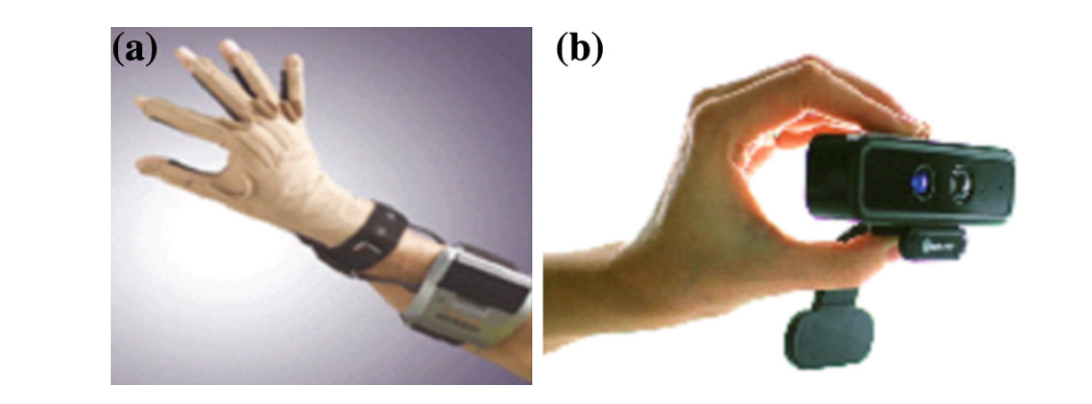
\includegraphics[width=0.6\linewidth]{fig1.png}
  \caption*{(a)基于触觉的手势识别:Cyber Glove II\cite{kevin2004};(b)基于计算机视觉的手势识别: SoftKinetic HD 相机\cite{iisuSDK2012}。}
  \caption{不同的手势识别技术}
  \label{fig:gesture_techniques}
\end{figure}

本研究观察到,RGB-D 手势识别的主要挑战可以归因于两个因素:(i)\textit{信息冗余 (IR)}。
在纠缠的时空空间中,冗余信息很难处理 \cite{zhou2023unified, LI2024110536}。利用耦合建模结构的模型通常会在训练期间学习背景、照明和表演者外观等不相关的特征 \cite{zhou2023unified},这可能会导致误导性分类 (图 ~\ref{fig:gap_sample})。尽管现有方法在训练数据集上表现良好,但在未见的场景中,它们的准确性会显著下降。这种差异凸显了一个关键的泛化问题,即模型在消除冗余信息方面遇到挑战,阻碍了与任务相关的细微手势特征提取。
(ii)\textit{信息缺失 (IA)}。模型难以区分具有高视觉相似性的手势 (图 ~\ref{fig:sim_sample})。虽然现有方法建议加入额外的线索,如姿势 \cite{wan2016chalearn,zuo2023natural} 和光流 \cite{narayana2018focus} 来增强手势识别,但这些方法的有效性仍然依赖于视觉,并且受到运动模糊和透视变化等问题的严重影响,特别是在区分视觉相似的手势时。
鉴于这些挑战,有必要开发一种有效的方法,最大限度地减少不相关的信息冗余,并解决整个手势识别过程中基本信息的缺失。

\begin{figure}[tb]
  \centering
  \subcaptionbox{同一手势类别具有不同的背景、照明和视角。\label{fig:gap_sample}}
  {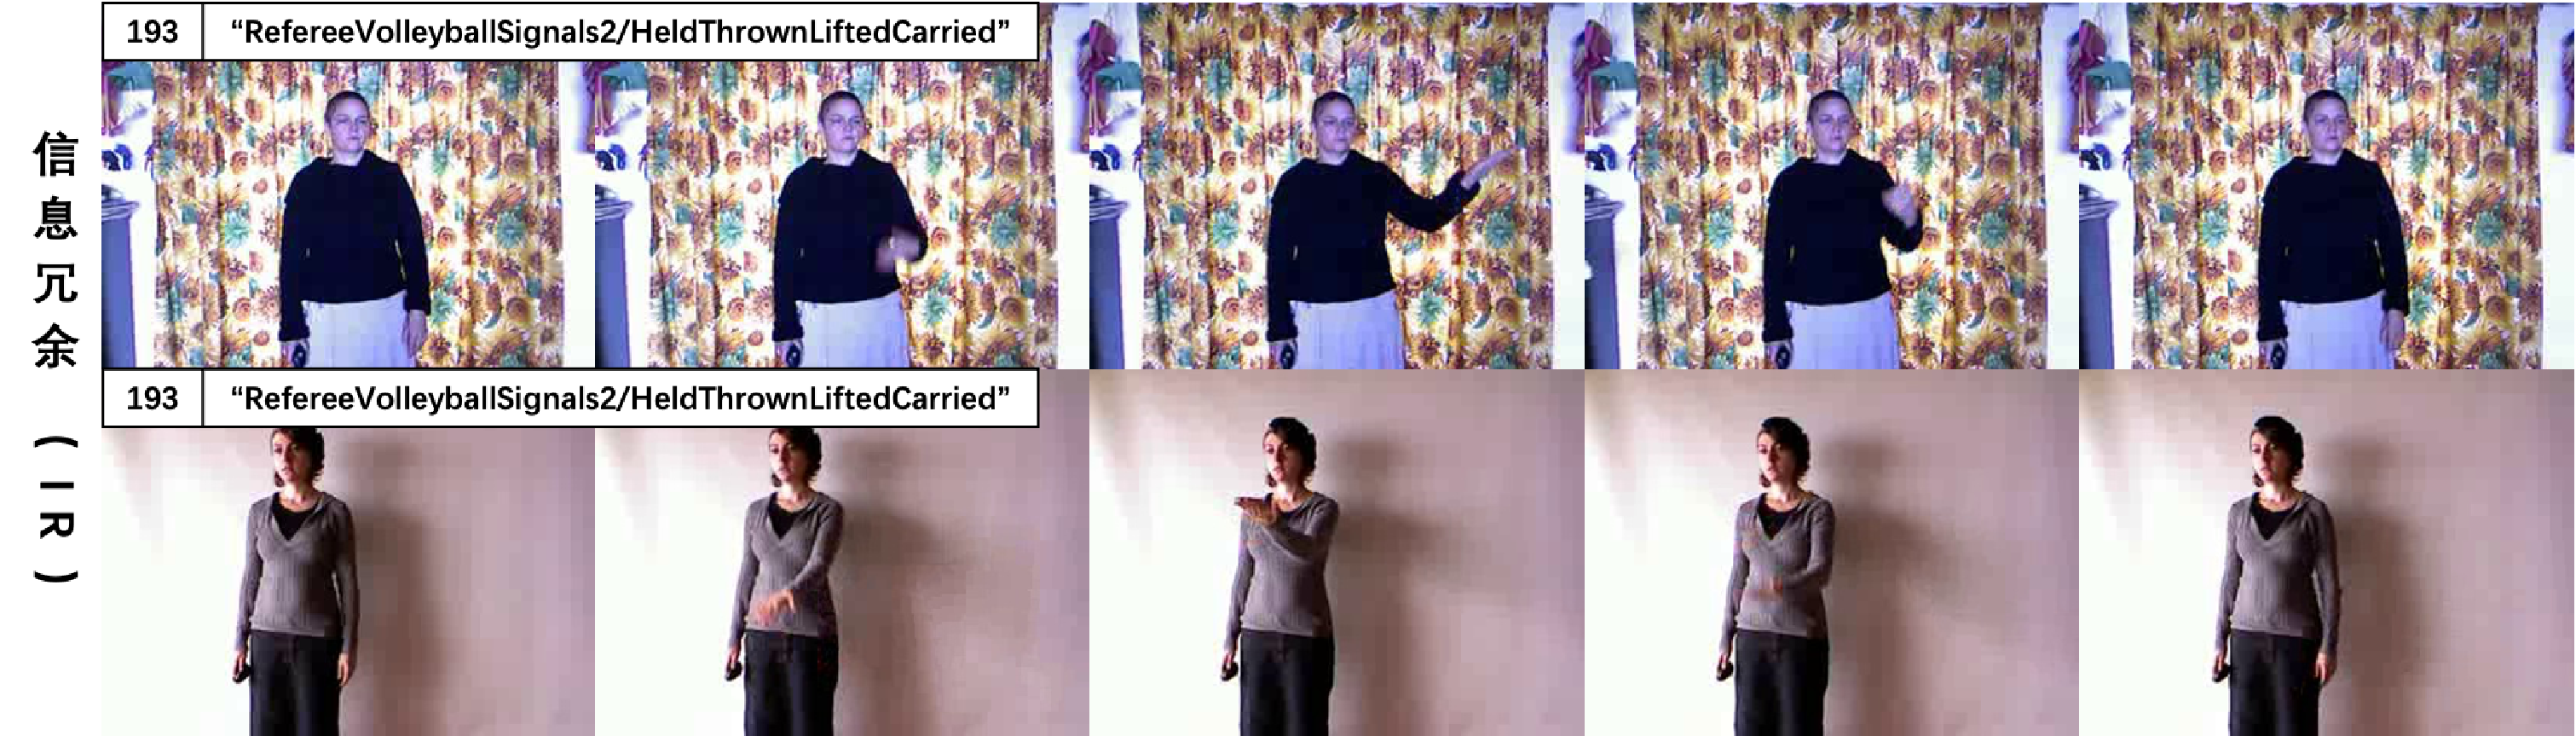
\includegraphics[width=1.0\linewidth]{IR.pdf}}
  \subcaptionbox{不同的手势类别具有视觉上相似的表示。\label{fig:sim_sample}}
  {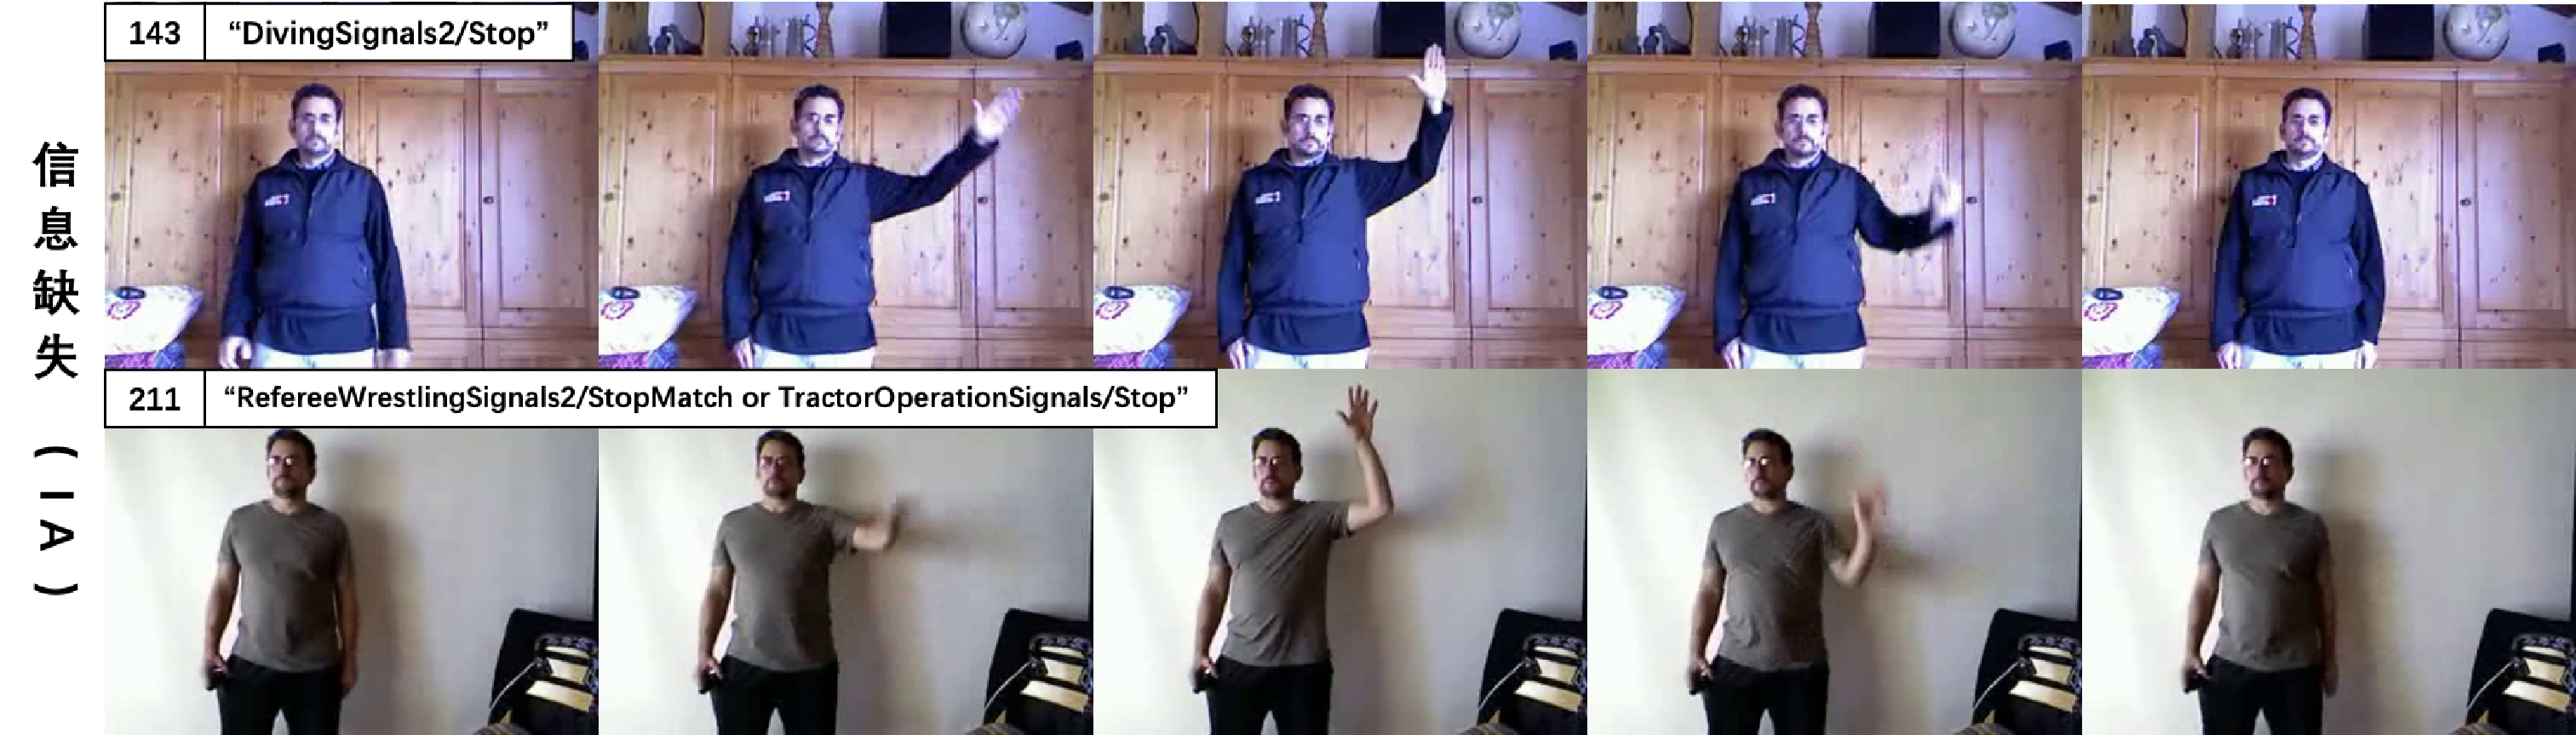
\includegraphics[width=1.0\linewidth]{IA.pdf}}
  \caption{RGB-D 手势识别的主要挑战可归因于两个因素:(i)\textbf{信息冗余 (IR)} 存在于类内,尤其是背景、照明和视角。(ii) \textbf{信息缺失 (IA)} 存在于类间,尤其是视觉上相似的手势。}
  \label{fig:samples}
  \end{figure}


\textbf{手势生成}因其在人机交互领域的广泛应用而备受关注,如虚拟现实、游戏和数字虚拟人等。为了增强手势生成的多样性和可控性,研究人员探索了多种模态,包括语音~\cite{yang2023diffusestylegesture, yang2023unifiedgesture,xu2025mambatalk}、文本转录~\cite{zhi2023livelyspeaker, pang2023bodyformer,liu2024emage}、情感~\cite{qi2024emotiongesture, qi2024weakly}、风格~\cite{ao2023gesturediffuclip, yang2023diffusestylegesture, ghorbani2023zeroeggs}以及说话者身份~\cite{yang2023diffusestylegesture+}等。其中,语音同步性和语义相关性是两个备受关注的关键方面。尽管深度神经网络~\cite{liu2024emage, xu2025mambatalk, cheng2024siggesture}的进步显著提高了生成质量和多样性,但当前的方法主要关注自发性的伴随语音手势,而忽视了文本驱动的非自发性手势~\cite{yang2024freetalker}。这通常导致虚拟人动作的模糊性~\cite{chen2024syntalker},并限制了通过文本提示控制生成动作的灵活性,阻碍了手势生成算法的实际应用。

一个关键挑战在于现有手势数据集缺乏直接的描述性文本标注:虽然语音数据自然且直接可用,但语义相关性通常仅通过语音转录推断,导致语义关联较弱。此外,手动标注手势语义成本过高,这阻碍了高质量生成和精细化的说话者语义控制。虽然一些方法尝试通过引入额外的动作数据集进行联合训练来缓解这一问题~\cite{yang2024freetalker},但它们仍然存在手势数据的语义差距,只能在两个任务之间切换而非实现联合控制。另一种潜在的解决方案是通过动作-文本对齐预训练构建对齐的嵌入空间,以获取手势的隐式文本标签~\cite{chen2024syntalker},但这会引入额外的训练和推理成本。此外,由于人体动作数据集和手势数据集之间存在显著的分布差异~\cite{chen2024syntalker},联合嵌入空间的泛化能力仍有待验证。鉴于这些挑战,有必要开发一种有效的方法,既能解决手势数据标注缺失问题,又能实现多模态信号的协同生成控制,同时将成本降至最低。


基于上述背景,本文致力于提出一种新颖的多模态手势识别与手势生成算法,并基于此开发一个交互式手语学习助手系统。首先,通过引入一种多策略解耦与语义集成手势识别网络,实现手势识别的准确性提升;其次,通过提出一种描述驱动的协同手势生成网络,增强手势生成的描述性控制;最后,通过在手语学习系统中集成手势识别和生成算法,实现手语动作的智能评估和标准动作库的动态扩充生成。该系统能够有效缓解手语教学资源匮乏的问题,提升自主手语学习的效率和质量,还可以为听障人士的日常交流提供有力的技术支持,具有重要的社会价值和广阔的应用前景。



\section{国内外研究现状综述}
\subsection{多模态动态手势识别}
\subsubsection{手势识别概述}
% 手势
根据文献研究\cite{kaaniche2009gesture, rautaray2015vision},手势可分为静态和动态两大类。前者指手部在空间中保持固定姿态不动,后者则涉及手部在时空中的变化过程。动态手势可进一步细分为五个子类别\cite{ottenheimer2018anthropology}:标志,情感展示,调节器,适配器和解释器。图\ref{fig:gesture_taxonomies}显示了手势类别的分类学。由于动态手势中往往包含更丰富的语义表示,近年来更多的研究围绕动态手势展开。
\begin{figure}
  \centering
  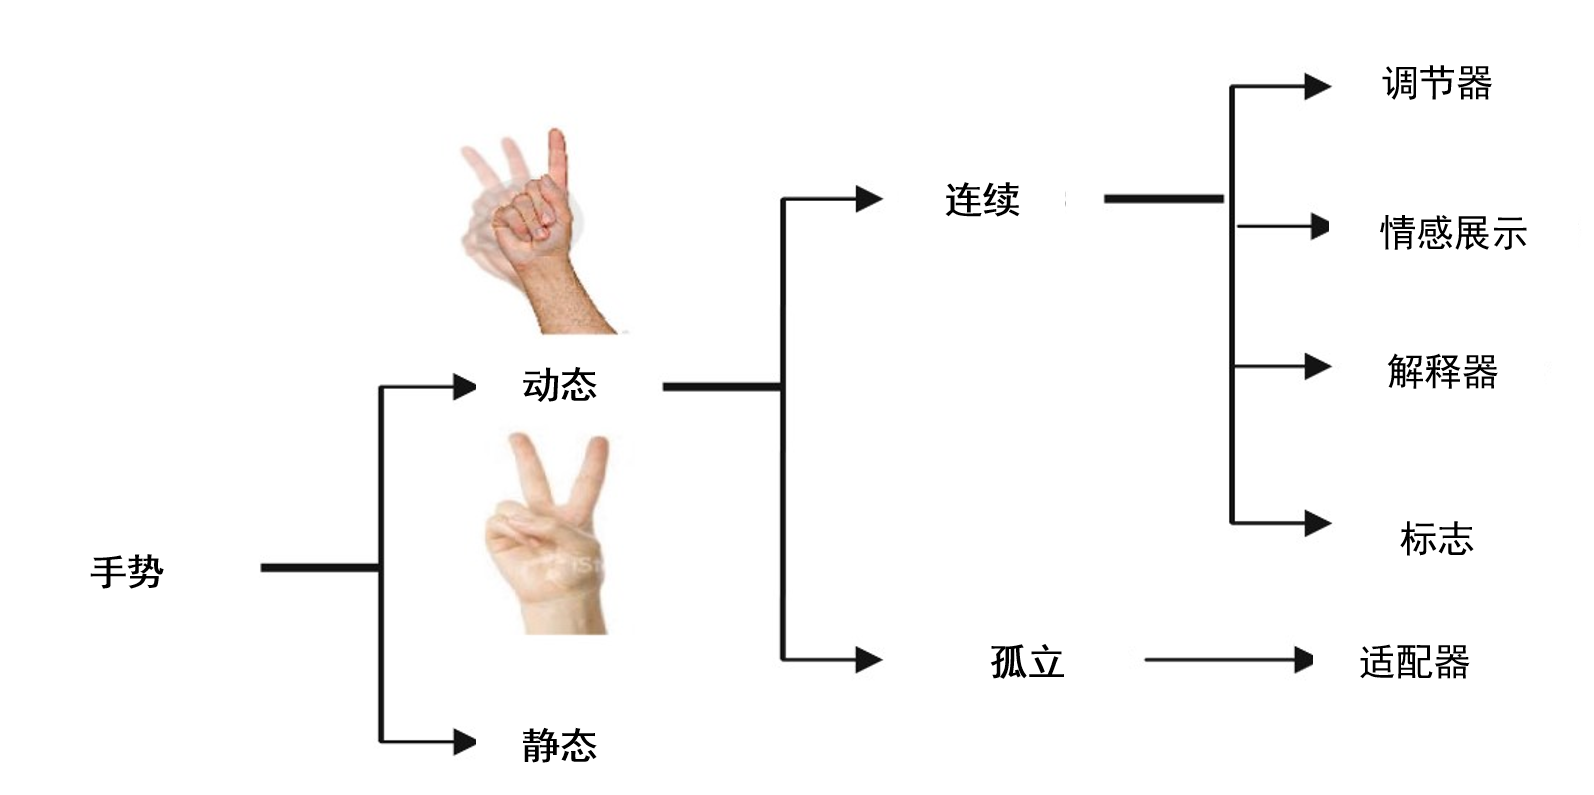
\includegraphics[width=0.9\linewidth]{fig2.png}
  % \caption*{}
  \caption{基于视觉的手势分类法\cite{rautaray2015vision}}
  \label{fig:gesture_taxonomies}
\end{figure}

% 手势识别
手势识别是一个完整的过程,涉及跟踪手势、识别其含义并将其转化为有意义的指令\cite{rautaray2015vision}。
%% 触觉、视觉
手势识别技术主要包括触觉式和视觉式两大类\cite{oudah2020hand,rautaray2015vision}。
触觉式识别通过可穿戴设备采集手部运动数据,经由计算设备分析处理后完成识别。常用的接触式传感方法包括:数据手套、手部光学标记、加速度计、触摸屏、表面肌电等\cite{oudah2020hand}。
尽管基于数据手套的方法具有可穿戴、灵活便捷等优势,但它们也有许多局限。例如:基于接触的设备并没有给用户提供太多的可接受性\cite{rautaray2015vision},并且不适合老年人;电线连接会影响设备的灵活性;长时间使用也受到设备寿命的限制;此外,一些传感器可能相当昂贵\cite{oudah2020hand}。
视觉手势识别是通过相机等视觉传感器捕捉手势的形状和动作,并运用计算机视觉技术对2D和3D手势进行识别的过程。
常用的视觉相机设备包括2D摄像头、Kinect、LeapMotion、Time of Flight (ToF) 相机等\cite{基于视觉的动态手势识别研究综述}。
尽管视觉手势识别容易受到遮挡、光照等问题的干扰,但由于其具有用户友好、设备易得的优势,因此视觉手势识别成为近年来研究的主流方向。

本研究将深入探讨基于视觉的动态手势识别,探讨多模态识别过程中的特征解耦与融合,通过引入先进的深度学习技术进一步提升识别的准确性和鲁棒性。
%此外,由于手势动作往往涉及相当多的自由度(DoF),即使是相同的手势在不同视点下也会发生2D外观的巨大变化,不同的手势动作可能存在不同的空间分辨率与手势速度\cite{rautaray2015vision},不同的背景与手势表演者也会给识别增添困难...... ,因而视觉手势识别研究对于科研人员来说仍然具备相当多的挑战性\cite{基于视觉的动态手势识别研究综述}。
%% 动态、静态
%% 连续、孤立
% 输入模态
% ...
% 文献评述

\subsubsection{基于手工提取特征的手势识别方法}
% ref: rautaray2015vision
% ref: 基于视觉的动态手势识别研究综述
早期研究使用手工提取特征进行手势识别,包括检测、追踪和识别三个阶段\cite{rautaray2015vision}。
检测的目的是进行手的检测和相应图像区域的分割,常基于肤色\cite{sigal2004skin}、形状\cite{chen2007real}、3D模型\cite{tekin2019h+}、运动\cite{pun2011real}、骨架\cite{jiang2021chal21}等特征进行手部检测。
追踪技术旨在获取手部在连续帧中的位置信息,构建动态轨迹特征。通过对这些包含手势基本信息的轨迹进行分析,可实现对手势类型的识别与理解。
基于模板的方法(Template based)\cite{crowley1995finger}与手部检测方法非常相似。此类方法在前一帧中检测到手的空间附近调用手检测器,从而在很大程度上限制图像搜索空间,但要求图像具有足够的采样帧率。基于最佳估计的方法(Optimal estimation)\cite{argyros2004real}采用卡尔曼滤波器\cite{kalman1960new}提供的最优估计框架具有实时的性能并能为连续帧提供预测。基于粒子过滤(Particle filtering)的方法\cite{perez2002color}被用来在密集的视觉混乱中跟踪手的位置和手指的配置,此类方法用一组粒子建模手的位置,对于复杂的模型需要更多的粒子。
基于连续自适应均值偏移(CamShift)的方法\cite{wang2010study}参考了基于核的mean shift算法原理,它通过迭代计算来寻找目标的分布中心,并可动态调整跟踪窗口尺寸,实现对目标的自适应跟踪。
CamShift具有轻量、鲁棒、高效的优点,但在复杂场景中容易失败、且容易发生窗口漂移问题。
识别阶段的目标是对手的位置、姿势提供最终的语义解释。静态手势识别可以使用模板匹配或基于机器学习的简单分类器\cite{基于视觉的动态手势识别研究综述},如:支持向量机(SVM)\cite{burges1998tutorial}、随机森林\cite{基于视觉的动态手势识别研究综述}、K近邻算法(KNN)\cite{thirumuruganathan2010knn}等。动态手势识别则需要对时间维度进行建模,隐马尔科夫模型(HMM)\cite{liang1996sign},动态时间规整(DTW)\cite{corradini2001dynamic},时延神经网络\cite{sigal2004skin}等算法在动态手势识别系统中得到了广泛的应用。
传统手势识别方法的关键在于如何合理地提取手工特征,具有计算成本低、速度快的优势。但由于过于依赖于技术人员经验与精巧的模型设计,算法的泛化性、鲁棒性往往较差。

\subsubsection{基于深度学习的手势识别方法} % (时空建模)
伴随着计算能力的提升以及大规模多模态数据的积累,基于深度学习的手势识别技术实现了重大突破。
与传统算法相比,深度学习不仅减少了对手工工程的需求,而且提升了算法的准确性、适用性与效率。因此,基于深度学习的手势识别方法已经成为该领域的主流研究方向,受到广泛关注。

% \paragraph{基于RGB-D的动态手势识别}
% ref: 基于视觉的实时手势识别方法(2019大连理工)
% RGB
%% 2DCNN
卷积神经网络(CNN)已被证明是许多计算机视觉任务中的有效算法,2DCNN方法被广泛用于处理静态手势图像的分类和识别任务。这些网络通过卷积层和池化层有效地捕获图像中的空间特征。
%% Two stream
针对视频中的动态手势动作,早期研究者试图在时域中扩展 2DCNN 的连接性以进行视频分类\cite{karpathy2014large}。Simonyan等人\cite{simonyan2014twostream}提出了双流神经网络(Two Stream CNN)来分别学习空间和时间特征,其中空间流处理静态单帧图像,时间流则处理多帧光流。
TSN\cite{wang2016tsn}在双流卷积神经网络的基础上进行稀疏时间采样,所提出的时间段网络可以对整个动作视频进行高效的学习。
TRN\cite{zhou2018trn}进一步改进了TSN中的融合方式,并提出了时间维度上的多尺度特征融合,以提升算法的鲁棒性。
2DCNN结构简单,但存在时域信息建模的不足;而双流方法依赖于预先提取的密集光流进行运动表示,网络同样缺乏有效的时域特征提取模块。

%% 3DCNN
受图像识别领域卷积神经网络突破的启发,3DCNN被提出并广泛应用于视频理解任务。
C3D网络\cite{tran2015c3d}通过在时空维度上扩展二维卷积核,实现了对视频序列中时空特征的直接提取,该网络在多种视频分析任务中展现出优异的性能。
此后,一系列基于3DCNN的神经网络被提出,并逐渐成为视频理解任务中的主流选择。
Carreira等人\cite{carreira2017i3d}结合了双流神经网络与3DCNN的优势,引入了一种新的双流膨胀 3D ConvNet (I3D)进行时空建模,在Kinetics动作视频数据集上实现了最先进的水平。
R2+1D\cite{tran2018r2+1d}通过将3D卷积分解为2D空间卷积和1D时间卷积的方式,实现了更高效的时空特征提取。
S3D\cite{xie2018s3d}考虑速度与准确度之间的平衡,将I3D与时空分离卷积结合,并引入一种特征门控机制以进一步提升网络的识别准确率。
Zhang等人提出了Deformable 3DCNN\cite{zhang2020deformable3d},通过所设计的轻量级时空可变形卷积模块,通过根据前序特征图学习额外的偏移量来增强3D卷积的时空采样位置,以减轻手势识别中背景的干扰。
3DCNN能够有效提取视频中的局部时空特征,但对长序列数据的建模能力较弱。此外,当网络输入较长时,往往需要更多层或更大的内核和步幅大小,增加了网络计算成本的同时也容易出现过拟合现象。

%% Recurrent
循环神经网络(RNN)\cite{jozefowicz2015empirical}和长短期记忆网络(LSTM)\cite{yue2015beyond}在序列数据处理中得到广泛应用。
这一特点促使研究人员将 CNN 和 RNN/LSTM 的优势结合起来,先后学习局部和全局特征。
长期循环卷积网络(LRCN)\cite{donahue2015lrcn}结合CNN和LSTM分别处理空间与时间特征,所提出的方法在动作识别、图像描述与视频描述多任务中取得了有竞争力的结果。
Molchanov\cite{molchanov2016online}和Cao\cite{cao2017egocentric}等人分别将3DCNN与循环神经网络(RNN)和长短期记忆网络(LSTM)相结合以进行端到端的手势识别,前者可以从多模态数据中同时检测和分类动态手势,后者针对自我中心手势识别任务,引入了一个循环时空转换模型,实现了3D特征的时空规范化。

%%% ConvLSTM
由于全连接长短期记忆网络(FC-LSTM)难以提取数据中的空间特征,Shi等人\cite{shi2015convlstm}提出了卷积长短期记忆网络 (ConvLSTM) 来处理连续图像以进行临近降水预报。
研究表明,相比LSTM,ConvLSTM能更有效地捕获时空特征,并已在动作识别、手势识别等多个视觉任务中得到成功应用。
Zhu等人\cite{zhu2017multimodal}提出了一种基于3D卷积和ConvLSTM的孤立手势识别方法。该方法首先利用3DCNN提取短期时空特征,随后通过ConvLSTM建模长期时空依赖关系,并采用SPP\cite{he2015spatial}对特征进行归一化。该方法分别在RGB和深度模态上训练,最终通过平均融合得到预测结果。
在此基础上,Zhang等人\cite{zhang2017learning}提出了3DCNN+BiConvLSTM+2DCNN网络用于孤立手势识别。具体地,文章引入了双向卷积长短期记忆网络(BiConvLSTM)以替换网络中的ConvLSTM,并引入额外的2DCNN学习更高层次的时空特征。
AttnConvLSTM\cite{zhang2018attention}与
ConvLSTMForGR\cite{zhu2019redundancy}分析了ConvLSTM结构中的冗余问题,
% 研究表明,四个门结构中的空间卷积对时空特征融合贡献有限,而在输入输出门中嵌入的注意力机制也未能显著提升性能。
并进一步提出了一种改进的GatedConvLSTM变体,该模型只在输入到状态的转换过程中保留卷积操作。
对于未经分割的手势视频,Zhu等人\cite{zhu2018continuous}进一步将类似网络应用于连续手势识别,并提出了一种两阶段的连续手势识别方法。在分割阶段,使用时间扩张三维卷积神经网络将连续手势序列分割成孤立的手势实例;在识别阶段,则使用基于3DCNN+ConvLSTM+2DCNN的孤立手势识别网络进行识别分类。
基于循环神经网络的动态手势识别方法能够有效进行长期时间建模。然而由于手势视频中不同阶段的帧往往具有不同的重要性\cite{lin2018large},此类方法因为缺少时域上的注意机制,难以对不同重要性的视频帧进行有效建模。
另外,这类网络的计算效率也受到限制,因为每个时间步的计算都需要等待前一步的结果。

Transformer架构\cite{vaswani2017attention}可以通过注意机制更好地捕获上下文信息。
Vision Transformer(ViT) \cite{vit2021image}是一项开创性的工作,通过将视觉数据作为序列处理,而不是依赖于传统的卷积网络,引入了图像分类的新范式转变。
受ViT的启发,Video Transformer(VT)\cite{selva2023video} 通过引入额外的时间维度进行时空建模与视频理解。
TimeSformer\cite{bertasius2021space}率先使用纯Transformer结构用于视频识别。ViViT\cite{arnab2021vivit}探索了几种不同的时空注意力分解变体,验证了时空编码器分离方法的有效性。VTN\cite{neimark2021video}同样采用时空编码器分离的方式,并进一步引入Longformer实现复杂度为O(n)的长序列建模。
该机制通过滑动窗口实现局部上下文的自注意力计算,并结合任务相关的全局注意力机制。
Video Transformer(VT)方法已经在行为识别等视频理解领域取得了显著的成功,然而目前却少有研究将Video Transformer方法应用于手势识别领域来解决动态手势的分类问题。这可能是由于Video Transformer在计算复杂性方面面临着挑战,通常需要大量的计算资源和大规模的数据集来实现最佳性能\cite{khan2022transformers}。

% 受上述工作的启发,本研究将循环神经网络(ConvLSTM)与视频变换器(VT)的优势结合起来,引入了一种基于循环的手势识别变换器(RGRT,Recurrent Gesture Recognition Transformer),以实现多尺度的时空注意力建模。本研究利用时域窗口变换器(TWT,Temporal Window Transformer)在局部片段内进行并行计算,在全局视频范围内则使用基于卷积长短期记忆网络的循环结构进行长期建模,从而在保证计算效率的同时提升网络的识别性能。
与以前利用耦合建模结构来处理纠结的跨模态特征的方法相比,本研究侧重于两个解耦维度中的多模态特征的相互作用,并且可以无缝集成到各种 RGB-D 方法中。


% \subsubsection{\textcolor{red}{基于三维骨骼数据的手势识别}}
% %多模态:skeleton,点云,...
% 随着更多的多模态手势数据集被提出,除了主流的基于RGB-D视频的手势识别方法外,近年来也涌现出了许多基于3D骨架、点云等模态数据的方法。
% Aich等人提出了一种基于无数据类增量学习的三维骨骼序列手势识别方法(DFCIL)\cite{aich2023data},并引入了一种简单有效的用于DFCIL模型反演的边界感知原型采样机制。
% Liu等人\cite{liu2023temporal}则提出了一种时间解耦图卷积网络(TD-GCN)进行三维骨骼序列手势识别,它对来自不同帧的骨架应用不同的邻接矩阵。
% Min等人\cite{min2020efficient}将手势识别作为一个不规则序列识别问题,旨在捕获点云序列之间的长期空间相关性。所提出的PointLSTM在多个骨架数据集上取得了具有竞争力的结果。
% %% 解耦 Decoupled
% Bigalke等人\cite{bigalke2021fusing}认为直接处理三维点云序列有利于手势识别,并提出了一种解耦的双流模型分别进行局部姿势特征与全局运动特征的学习,多尺度的特征最终被融合在LSTM中用于时间建模。
% 类似地,Liu等人\cite{liu2020decoupled}提出了一个解耦的端到端双流网络进行基于骨骼的手势识别。网络将手势解耦为手部姿势变化和手部运动,然后分别建模。对于前者,骨架序列被嵌入到3D手部姿势演化体(HPEV)中使用3DCNN提取细粒度的姿势变化特征;对于后者,手中心和指尖的移动被安排为一个2D手部运动图(HMM),使用2DCNN捕捉整体运动;并最终将两个流的预测结果聚合。

% % 文献评述
% % \subsubsection{基于解耦的动态手势识别}
% 文献\cite{bigalke2021fusing, liu2020decoupled}已经明确指出,对于动态手势的解耦对提升手势识别性能具有积极作用。目前,解耦手势识别的研究主要集中在三维骨架手势方面,然而,三维骨骼数据的获取成本较高,需要依赖于上游的三维人体姿态识别算法或大量人工标注,限制了其在实际应用中的推广。相比之下,目前尚未有专注于二维手势视频的解耦手势识别研究。

\subsubsection{解耦手势特征学习}
由于复合手势特征在纠缠空间\cite{zhou2023unified,LI2024110536}中难以处理,一些研究人员尝试从各个角度解耦复杂手势特征学习,以提高识别性能。
一些工作\cite{zhou2022decoupling,LI2024110536} 尝试将“时空”手势特征空间解耦。
Zhou 等人 \cite{zhou2023unified} 提出了一种解耦时空表示学习网络 (DSN, DTN) 来学习特定于维度的表示。
然而,明确地隔离整个网络的时空维度可能会破坏特征的时空连通性,从而损害模型捕获隐式关节时空信息的能力。
% pose-motion
其他一些研究侧重于将 3D 手势表示与 3D 骨架或点云数据解耦。
Guo 等人 \cite{GUO2021108044} 强调,可以从两个角度看到手部骨架:显式关节云和隐式骨架拓扑。
Liu 等人\cite{liu2020decoupled} 提出,各种手势类别在对不同尺度特征的依赖方面表现出多样性。
Bigalke 等人 \cite{bigalke2021fusing} 提出了一种解耦的双流模型,用于从 3D 点云序列中独立学习局部姿势特征和全局运动特征。
然而,这种方法受到高数据收集成本的限制,对实际应用提出了挑战。
本研究试图同时将 RGB-D 手势与两个范例分离:i) 姿势-运动解耦 (PMD) 和 ii) 空间-时间-通道解耦 (STCD)。
这种方法有效地将细微特征集成到两个子空间中,同时保留了联合特征,使其有别于其他方法。

\subsubsection{多模态视觉-语言模型}
随着多模态领域的蓬勃发展,大量视觉语言模型 \cite{radford2021learning, li2022blip} 应运而生,并被应用于各种任务,例如,图像文本匹配和图像文本检索。
CLIP \cite{radford2021learning} 是该领域的开创性工作之一,利用大规模图像文本对进行训练,共同优化文本编码器和视觉编码器,以实现图像和语义特征对齐。
鉴于 CLIP 依赖于大规模预训练,一些研究人员旨在基于 CLIP 进行微调,以实现高效的少样本迁移和领域泛化 \cite{gao2024clip}。
Zuo 等人 \cite{zuo2023natural} 避免使用密集文本编码器,而是选择使用 fastText 来提取词级嵌入,以利用注释(符号标签)中包含的隐性知识。
手势本身具有自然的语义属性;然而,使用简单的词级嵌入不足以捕捉手势注释的复杂性。
在这一努力中,本研究首先将语义引入手势识别,利用预先训练的 CLIP 和适配器从手势注释线索中提取更丰富的语义,并促进语义视觉特征的充分交互,这与以前的视觉语言模型不同。


% 本文旨在填补基于二维手势视频的解耦手势识别研究领域的空白。通过采用手势分割方法并引入一种基于手部骨架弯折编码的手势表示(SBCGR),本研究将动态手势视频解耦为细粒度的局部姿势变化和粗粒度的手部运动。对于这些不同尺度的特征,本研究采用多流网络进行特征提取与识别。这一研究框架不仅能够为视觉动态手势识别领域提供关于基于二维数据的手势解耦方法的新见解,还能够丰富动态手势识别算法的应用场景。



\subsection{协同手势运动生成}

\subsubsection{手势生成概述}
手势生成任务是从多模态数据中生成手势动作序列的复杂任务。为了实现更多样、可控的协同语音手势生成,多模态数据被辅助建模,包括语音音频~\cite{yang2023diffusestylegesture, yang2023unifiedgesture,xu2025mambatalk}、文本转录~\cite{zhi2023livelyspeaker, pang2023bodyformer,liu2024emage}、情感~\cite{qi2024emotiongesture, qi2024weakly}、风格~\cite{ao2023gesturediffuclip, yang2023diffusestylegesture, ghorbani2023zeroeggs}、说话人ID~\cite{yang2023diffusestylegesture+}。其中,语音同步性和语义相关性是两个关键方面。由于语音数据的自然可获得性,协同语音手势生成一直是主要的研究重点。然而,由于手势数据集缺乏直接的描述性文本标注,语义相关性通常只能通过语音转录来推断,这限制了语义关联的强度。
Yang等人\cite{yang2024freetalker}提出了一种协同语音和文本驱动的方法,但仍然受到标注不足的限制,且无法提供基于两种信号的协同生成。Chen等人\cite{chen2024syntalker}利用提示-动作对齐预训练来生成隐式文本标签,但引入了额外的训练和推理成本。与现有方法不同,本研究提出了一种联合描述和语音驱动的协同手势生成框架,在实现生成手势的语义相关性和节奏一致性的同时,保持低标注和计算成本。

\subsubsection{基于深度学习的手势生成方法}
传统方法依赖基于规则或统计模型来学习语音-手势映射,而深度学习方法利用神经网络来建模音频和手势之间的复杂关系\cite{nyatsanga2023comprehensive}。

早期方法主要采用RNN\cite{liu2022beat,yoon2020speech}进行手势序列建模。
Liu等人\cite{liu2022beat}提出了一个大规模身体-表情-音频-文本数据集 BEAT,它具有 76 小时的高质量多模态数据。基于此他们构建了一个级联运动网络 (CaMN),它由上述六种模态组成,这些模态以级联架构构建,用于手势合成。
Yoon等人\cite{yoon2020speech}引入了一种基于多模态上下文的手势生成方法,通过融合语音、文本和说话者特征来生成自然的手势动作。
但基于RNN的方法在捕获长期依赖性和计算效率方面存在诸多局限
。随后,Transformer\cite{zhi2023livelyspeaker, pang2023bodyformer}被引入以通过自注意力机制更好地建模时序关系。
Zhi等人\cite{zhi2023livelyspeaker}提出了一种语义感知的协同语音手势生成方法,该方法通过多个控制机制实现了灵活的手势合成。该方法采用两阶段策略:首先基于文本内容生成初始手势,随后利用音频信息对节奏进行精细调整。
Bodyformer\cite{pang2023bodyformer}提出了一个变分转换器来有效地模拟手势的概率分布,这可以在推理过程中产生不同的手势,并引入了一个模式位置嵌入层和一个模态内预训练方案来捕捉不同说话模式下的不同运动速度并缓解数据的稀缺性,以从有限的数据中学习语音和 3D 手势之间的复杂映射。
然而,Transformer首先于其相对于序列长度的二次方复杂度,带来了显著的计算挑战。
近期,MambaTalk\cite{xu2025mambatalk}首次将选择性状态空间模型(SSM)引入手势合成领域,通过线性时间计算实现了高效的序列建模。该方法实现了具有离散运动先验的两阶段建模策略,以提高手势的质量。利用基础 Mamba 块,通过多模态集成增强手势多样性和节奏。

为了提升生成质量和可控性,研究者开始探索基于潜变量的生成方法。一些方法采用VQ-VAE架构对手势动作进行离散编码,实现更高质量的手势生成。
EMAGE~\cite{liu2024emage} 利用四个合成VQ-VAE与掩码身体手势先验来提高结果的保真度和多样性,该研究同时引入了BEAT2(BEAT-SMPLX-FLAME),这是一个新的网格级整体共语音数据集,优化了头部、颈部和手指运动的建模,提供了社区标准化的高质量 3D 动作捕捉数据。
QPGesture~\cite{yang2023qpgesture}提出了一个手势 VQ-VAE 模块来学习codebook来总结有意义的手势单元。每个代码代表一个独特的手势,有效缓解了随机抖动问题。
TalkSHOW~\cite{yi2023generating}提出了一个新颖的语音到动作生成框架,其中分别对面部、身体和手进行建模,结合VQ-VAE和跨条件自回归模型(Gated PixelCNN)产生连贯且一致逼真的运动。

由于其强大的生成能力,扩散模型\cite{cheng2024siggesture,alexanderson2023listen,tevet2022mdm,yang2023diffusestylegesture}近期被广泛应用于运动和手势生成,显著增强了生成输出的多样性。
SIGGesture~\cite{cheng2024siggesture}通过大规模预训练扩散模型的语义注入进行泛化协同语音手势合成。该研究收集了一个名为LSMoG的大规模手势数据集进行预训练,时间长达400小时。
在运动生成领域,MotionDiffuse~\cite{zhang2024motiondiffuse}代表了第一个基于文本的运动扩散模型,该模型提供了对身体部位的细粒度指令,并实现了随时间变化的文本提示的任意长度的运动合成。
MDM~\cite{tevet2022mdm}引入了一种基于原始运动数据的运动扩散模型,实现了高质量的生成和通用的条件化,共同构成了新的运动生成任务的良好基线。
Yang等人~\cite{yang2023diffusestylegesture}使用使用扩散模型生成风格化音频驱动的协同语音手势,可以生成自然、语音匹配、风格一致的手势。
然而,现有基于扩散的方法通常直接在动作空间进行建模采样,导致计算开销大且训练不稳定。相比之下,潜在扩散模型(LDMs)\cite{rombach2022high}通过在低维潜空间进行操作,在保持强大生成能力的同时实现了计算效率。

与现有方法不同,本研究提出了一种基于描述增强的手势潜在扩散模型,该模型在保持低标注和计算成本的同时,实现了语义相关性和节奏一致性的双重目标。

\subsubsection{动作-文本转换}
人类动作展现出类似于自然语言的语义耦合,常被视为一种肢体语言形式~\cite{jiang2024motiongpt}。以往关于人体运动的研究探索了各种与文本相关的任务,包括文本到动作生成~\cite{tevet2022mdm,guo2022humanml3d}、动作到文本描述~\cite{jiang2024motiongpt,guo2022tm2t}以及统一的动作-语言建模~\cite{tevet2022motionclip,jiang2024motiongpt,jiang2024motionchain}。
近期的文本到动作工作(MDM~\cite{tevet2022mdm}、MLD~\cite{chen2023executing}、MotionLCM~\cite{dai2024motionlcm})利用预训练语言模型提取语义信息来控制动作生成。动作描述旨在使用自然语言描述人类动作,早期方法依赖统计模型和RNN来学习动作到语言的映射~\cite{takano2015statistical, yamada2018paired}。
近年来,双向动作-文本转换受到了更多关注。TM2T~\cite{guo2022tm2t}通过标记化首次实现了动作与文本的双向生成,尽管仅限于单一统一框架。随着大语言模型的发展,统一的动作-语言模型(如MotionGPT~\cite{jiang2024motiongpt}、MotionChain~\cite{jiang2024motionchain}、M3GPT~\cite{luo2024m})通过融合语言数据和大规模动作模型而涌现。

尽管手势本身具有自然的语义属性,但目前尚未有研究探索手势理解和描述生成。
为了解决这些局限性,本文首先探索了一种手势描述生成方法来填补手势数据中文本标注的空白,并开发了一种多粒度描述控制机制,实现对非自发手势的精确语义控制。



\subsection{基于手势的人机交互应用系统}
% Hand Gesture Recognition Based on Computer Vision: A Review of Techniques
% ref: 基于视觉的动态手势识别研究综述 解迎刚 1,2,王全 1
% ref: 伍杰2019基于视觉的实时手势识别方法研究
% ref: 审稿/人机交互.pdf
手势作为人与人之间交流的自然媒介形式,是人机交互最适合的形式之一\cite{oudah2020hand},基于手势的人机交互技术已经被广泛应用在各个领域。例如:

(1)机器人控制。 基于手势的人机交互,可被广泛用于机器人导航控制等领域\cite{al20223d}。国内无人机制造商大疆公司所发布的晓Spark的无人机可以识别用户手势,完成上下起降、左右移动和拍照等基本操作,极大的提高了用户体验(图~\ref{fig:3a})。

\begin{figure}
  \centering
  \subcaptionbox{大疆无人机晓 通过手势控制拍照\label{fig:3a}}
    {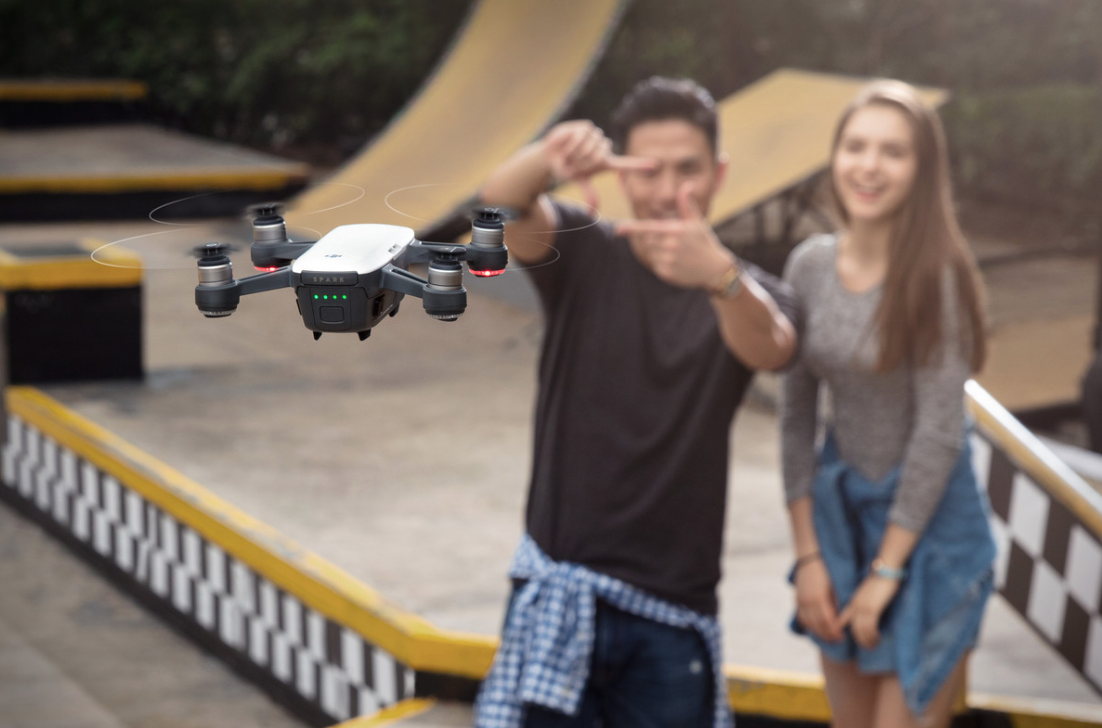
\includegraphics[width=0.4\linewidth]{fig3a.png}}
  \subcaptionbox{Oculus Quest手势追踪\label{fig:3b}}
    {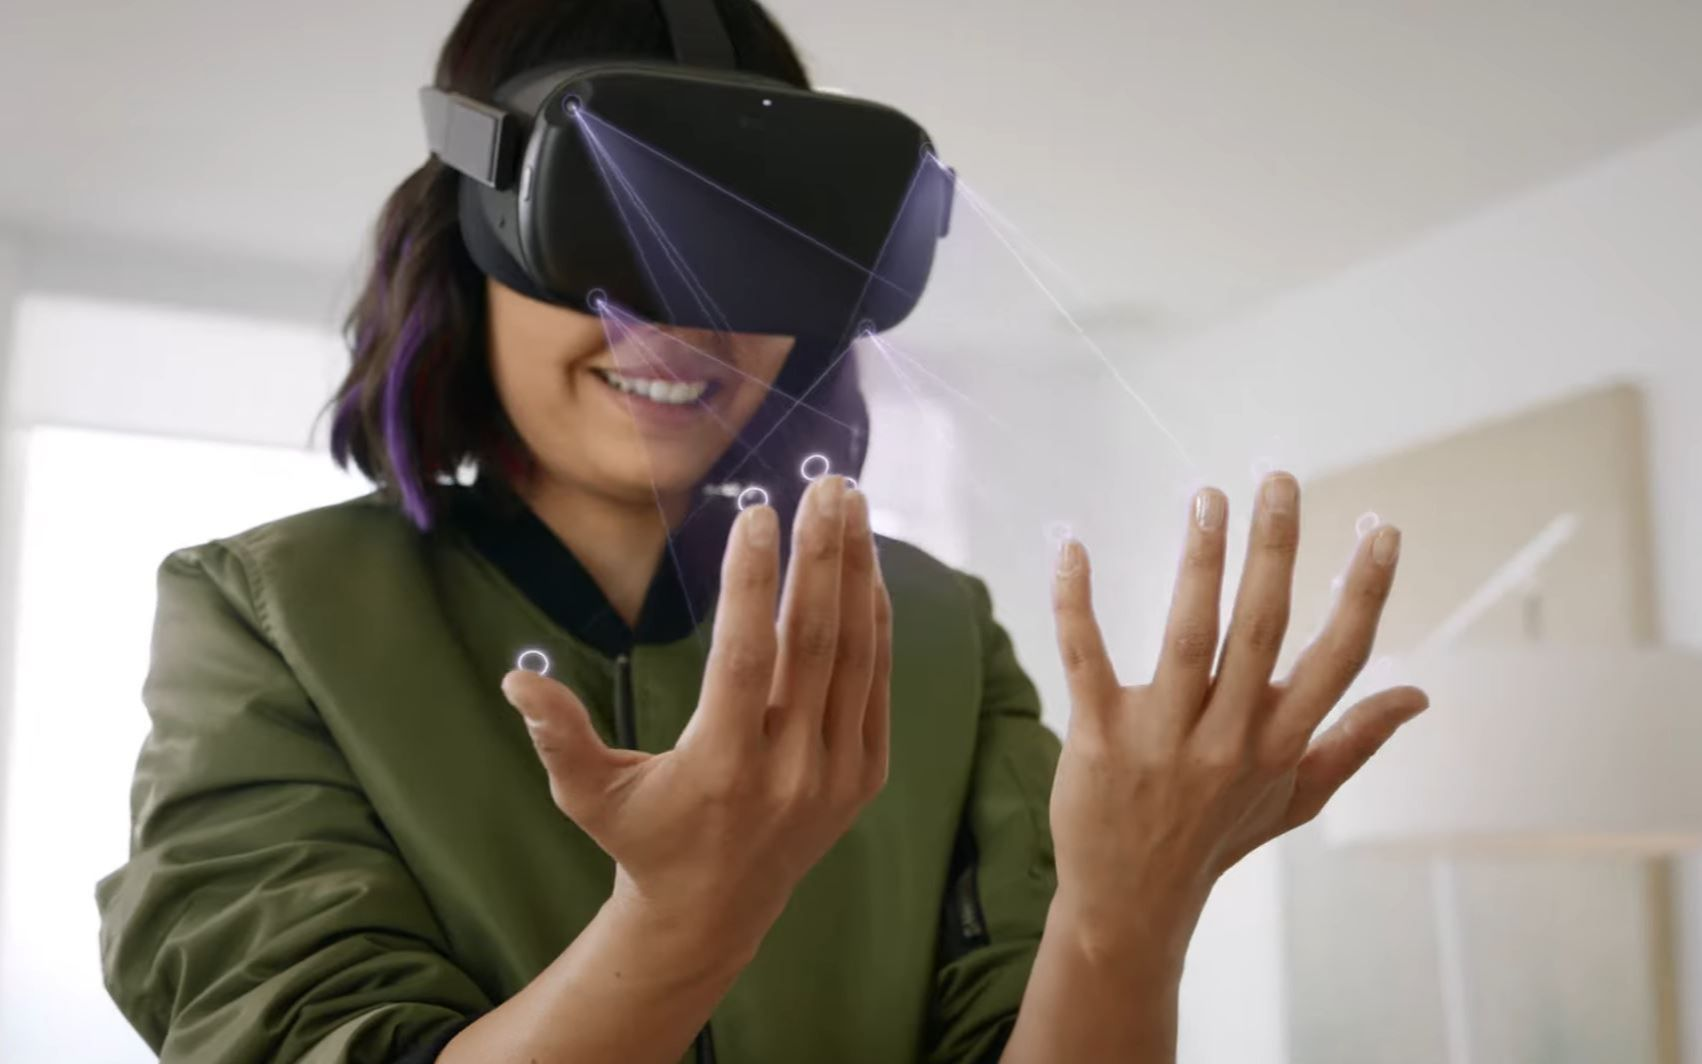
\includegraphics[width=0.4\linewidth]{fig3b.jpg}}
  \caption{基于手势识别的人机交互应用系统}
  \label{fig:HCI_system}
\end{figure}

(2)车载手势。Alba-Castro等基于手势识别技术, 构建了一个基于手势操作的车载娱乐媒体设备控制系统\cite{parada2014hand}。 Manawadu 等基于人车接口,利用手势识别的技术实现了自动驾驶汽车的经纬度控制\cite{manawadu2016hand}。
%[32] ALBA-CASTRO J L, GONZáLEZ-AGULLA E, PARADA-LOIRA F. Hand gestures to control infotainment equipment in cars[C]// Intelligent Vehicles Symposium. 2014. [33] MANAWADU U, KAMEZAKI M, ISHIKAWA M, et al. A hand gesture based driver-vehicle interface to control lateral and longitudinal motions of an autonomous vehicle[C]// IEEE International Conference on Systems. 2017.
% 宝马集团在 2015 年推出的车辆 iDrive 人机交互 指令系统,能够使用手势对车辆输入指令,如旋转手势进行音量调整、空中滑 动手指进行电话的接听等,实现对车辆的智能化控制。
% 君马 SEEK 5,9 种动态手势动作
% “Ez more 智能手势控制精灵” 

(3)智能家居。手势识别技术在家庭自动化领域具有广泛应用,可实现对照明系统、通风设备、视听设备等智能家电的便捷操控。
智能电视领域也开始应用手势识别技术,通过捕捉用户的手势动作实现对电视的远程控制。Desai等人的研究表示,相关技术可以用来改善老年人的生活质量\cite{desai2017human}。
% [64] DESAI S,DESAI A.Human computer interaction through hand gestures for home automation using Microsoft Kinect [C]//International Conference on Communication and Networks:Advances in Intelligent Systems and Computing. Singapore:Springer,2017,508:19-29

(4)手语翻译。聋哑人由于生理限制,无法使用声音进行交流,手势和手语成为了他们最依赖的沟通形式。然而,手语翻译是在实时翻译领域容易被忽略的交流形式\cite{SLR1}。近年来,手势识别在手语翻译系统中的应用研究得到了越来越多的关注\cite{伍杰2019基于视觉的实时手势识别方法研究}。
纽约大学的Li等人研发了一款名为“ASLR”的AR实时手语翻译应用原型\cite{SLR1}。该应用将计算机视觉与AR技术相结合,能够捕捉摄像头前执行的特定手语手势,并以用户的母语提供实时翻译(如图\ref{fig:SLRa}所示)。然而,由于该原型设计用于手机,用户在执行手语的过程中需要反复拿起和放下手机,增加了使用的负担。
Will等人构建了一个AR眼镜上的实时语音翻译系统原型\cite{SLR2}。该系统可以聆听语音,将其翻译成37种语言之一,并将生成的文本直接显示在用户眼镜上作为字幕。如图\ref{fig:SLRb}所示,用户可以在AR眼镜上享受实时的字幕翻译,同时自然地进行下棋等活动。这表明在AR眼镜上部署实时翻译应用是一种自然而灵活的方式。

\begin{figure}
  \centering
  \subcaptionbox{ASLR: 使用手机进行AR实时手语翻译的应用原型\label{fig:SLRa}}
    {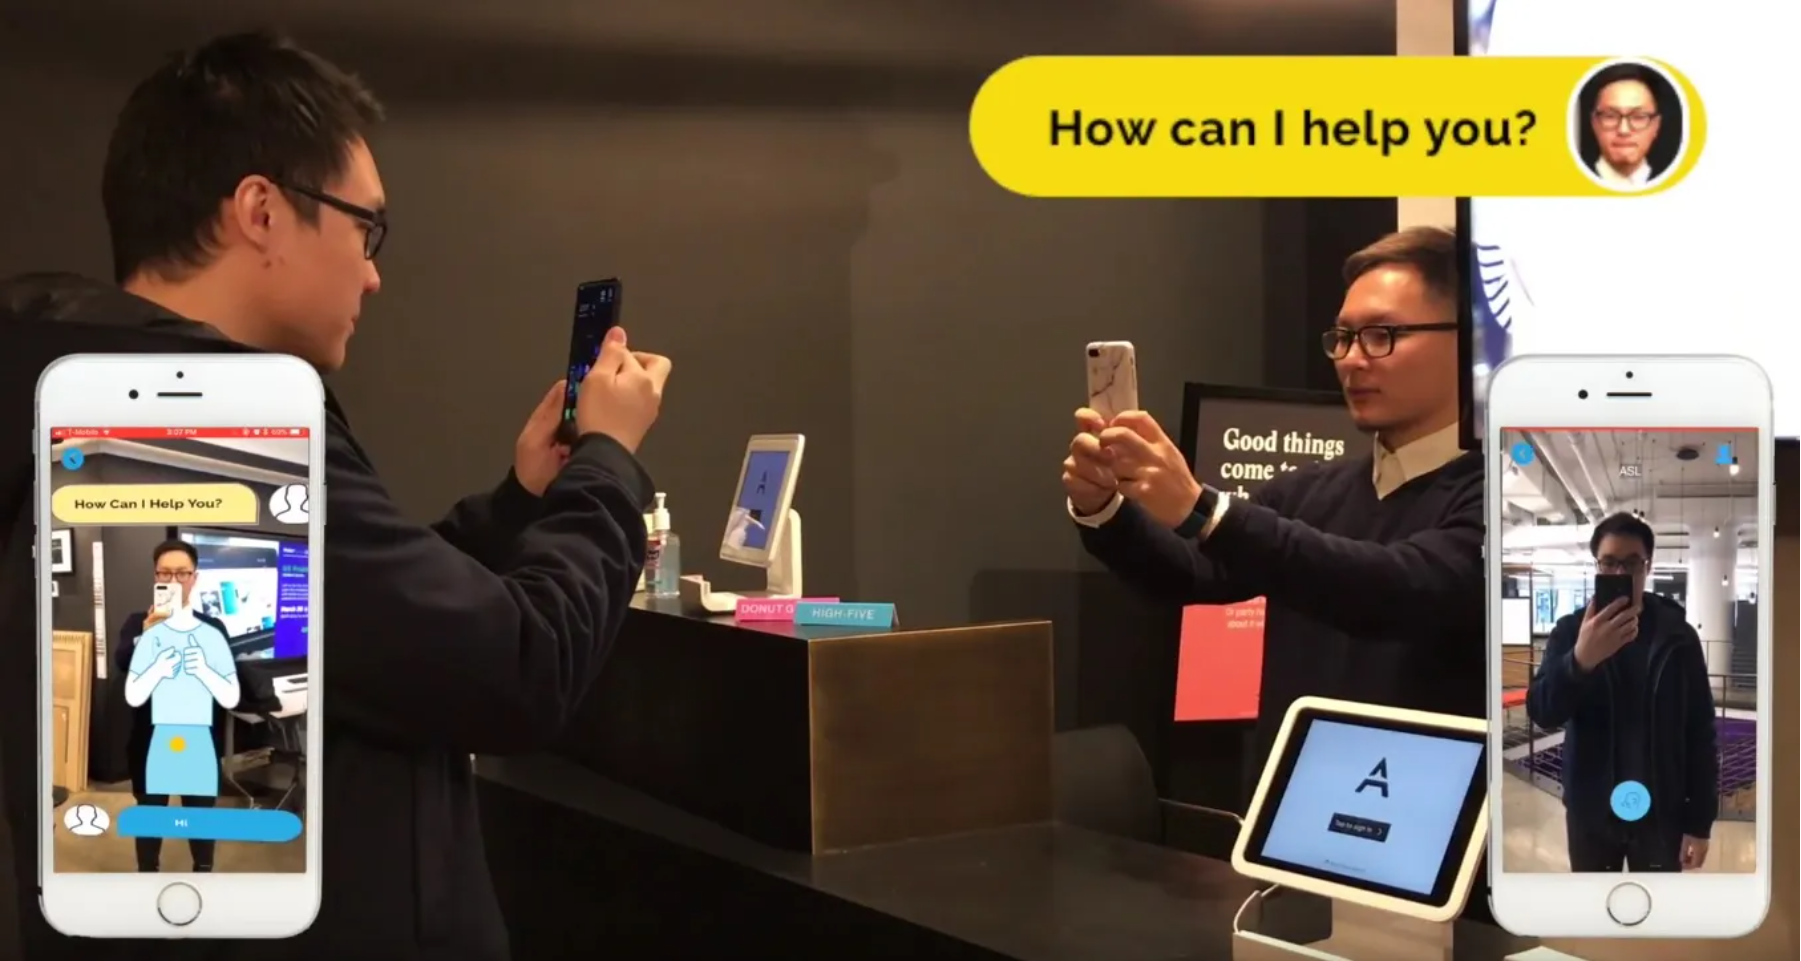
\includegraphics[width=0.45\linewidth]{ASLR.png}}
  \subcaptionbox{AR眼镜上的实时语音翻译应用\label{fig:SLRb}}
    {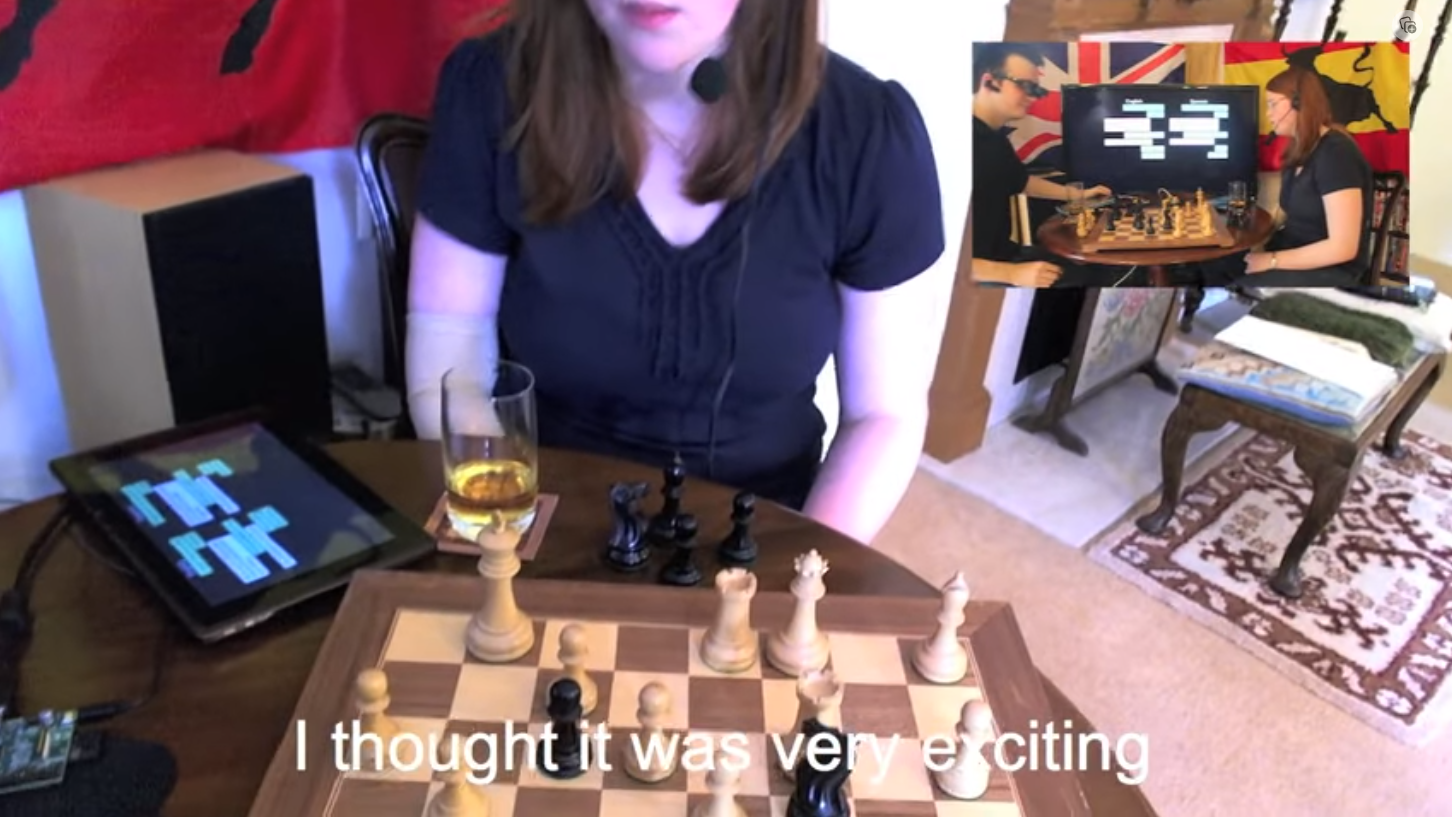
\includegraphics[width=0.45\linewidth]{SLRb2.png}}
  \caption{增强现实环境下的实时翻译应用}
  \label{fig:SLR}
\end{figure}

%【...】
%Birk 等设 计了一个准确率高达 99% 的实时手语识别系统,该系统采用主成分分析法对手势图像 进行特征提取,并基于欧几里德距离完成了贝叶斯分类器的训练[28]。Murugeswari 等基 于单目摄像头采集的图像,采用 SIFT 方法提取手势的关键点,然后使用向量量化将关 键点映射成统一维度的直方图向量,最后利用 SVM 多分类方法完成手势的分类[29]。国 内研究者张良国 等基于 Hausdorff 距离模板匹配的方法,在中国手语手指字母集上基于 单目视觉实现了识别 30 个手指字母的手势识别系统,平均识别率达到了 96.7%[30]。中 国科学与技术大学的黄杰基于三维卷积网络和注意力机制等深度学习方法,针对手语识 别中的孤立手语和连续手语识别进行了详细研究 [31] 。
%[28] BIRK H, MOESLUND T B. Recognizing gestures from the hand alphabet using principal component analysis[J]. 1996. [29] MURUGESWARI M, VELUCHAMY S. Hand gesture recognition system for real-time application[C]// International Conference on Advanced Communication Control & Computing Technologies. 2015. [30] 张良国, 吴江琴, 高文, 等. 基于 Hausdorff 距离的手势识别[J]. 中国图象图形学报, 2002, 7(11): 1144-1150. [31] 黄杰. 基于深度学习的手语识别技术研究[D]. 中国科学技术大学, 2018.

(5)虚拟现实交互。手势能够使用户与虚拟场景的交互更加自然方便,因此被广泛应用于增强现实、虚拟现实等环境中(图\ref{fig:3b})。Taylor等人使用手势识别系统对采集到的手势进行实时匹配以弹奏虚拟钢琴\cite{taylor2016efficient}。
%随着虚拟现实 VR(Virtual Reality)和增强现实 AR(Augmented Reality)技术的发展,用户对于虚拟场景的交互体验要求也越 来越高。手势识别技术的应用能够提升用户体验,使用户与虚拟场景的交互更 加自然方便,如实现三维立体影像操控、虚拟物品的拿取等。
% AR,VR中的手势输入...
% 弹奏虚拟钢琴。该手 势识别系统利用数据集与采集到的手势进行实时匹配[63]。
%[63] TAYLOR J,LUFF B,TOPALIAN A,et al.Efficient and precise interactive hand tracking through joint,continuous optimization of pose and correspondences[J]. ACM Transactions on Graphics,2016,35(4):143.

(6)游戏娱乐。手势识别技术在游戏领域(Kinect、Xbox)得到了广泛应用。例如,通过摄像头传感器捕捉玩家的手部和身体动作,实现与游戏的自然交互,提升游戏体验。
% 腾讯云神图·手势识别。25 种常见的静态手势

(7)临床与健康。手势识别技术可以帮助医生在手术室内实现非接触式操控医疗设备和影像系统\cite{strickland2013using}。同时,该技术也被应用于辅助行动不便人士的康复训练和日常生活,例如通过手势来控制智能轮椅\cite{zeng2012natural}。
% 在临床手术中,为了缩短手术时间或提高结果的精 确性,外科医生可能需要患者整个身体结构的细节或详 细的器官模型,通过使用医学成像系统,如MRI、CT 和 X-ray 系统来实现。这些系统从患者的身体中收集数 据,并将其作为详细的图像显示在高分辨率的电子大 屏。外科医生可以通过使用计算机视觉技术在摄像头 前做手势来观察图像的交互。这些手势能实现一些操 作,如缩放、旋转、图像裁剪和切换到下一张或上一张幻 灯片,而无需使用任何周边设备,如鼠标、键盘或触摸 屏。任何额外的设备都需要消毒,这对于键盘和触摸屏 来说可能很困难。
% 此外,手势可以用于辅助目的,如轮 椅控制[58]。
% [58] ZENG J H,SUN Y R,WANG F. A natural hand gesture system for intelligent human-computer interaction and medical assistance[C]//2012 Third Global Congress on Intelligent Systems,2012:382-385.
% 多伦多Sunnybrook医院[167]伦敦的盖伊和圣托马斯医院[168]都通过精心设计的三维手势此对,实现无菌环境中的非接触式操作。
% (167) Strickland M,Treraine J, Brigley G, et al. Using a depth-sensing infrared camera system to accessand manipulate medical maging from within the sterile operating field(J]. Canadian Journal ofSurgery, 2013,56(3): E1.[168] OHara K, Gonzalez G, Sellen A, et al. Touchless interaction in surgerylJ]. Communications of theACM,2014,57(1): 70-77.

(8)计算机交互。手势交互作为一种创新的人机界面形式,能够取代鼠标键盘等传统设备,为用户提供更加直观的界面操作体验\cite{starner1998real}。
% [65] STARNER T,WEAVER J,PENTLAND A.Real-time American sign language recognition using desk and wearable computer based video[J].IEEE Transactions on Pattern Analysisand Machine Intelligence ,1998,20(12):1371-1375.

% 文献评述
本研究将聚焦动态手势识别与手势生成算法在手语教学中的应用。基于构建的交互式手语学习助手系统,实现手语学习、辅助练习、实时反馈等功能。这不仅能够有效缓解手语教育师资与教学资源短缺的难题,还能提升手语教学中的人机交互体验,具有广泛的社会价值与应用潜力。
% \textcolor{red}{本研究将聚焦动态手势识别算法在机器人控制系统中的应用。结合本研究所提出的先进的多模态动态手势识别算法的优势,本研究首次尝试将手势识别应用部署于奥比中光机器人平台环境,构建手势识别控制系统。这不仅能够有效提升人机交互过程中的用户体验,还具有广泛的应用潜力。}

%结合Li\cite{SLR1}和Will\cite{SLR2}等人的设计优势,本研究首次尝试将实时手语翻译应用部署于可穿戴增强现实环境。与传统基于手机或电脑的翻译系统相比,基于增强现实眼镜的可穿戴手语翻译系统具备灵活、便携、自然、非侵入式的优势,可以广泛应用于“医疗急救\cite{2022signmedicial}、法律援助\cite{2021signlawyer2}、手语教学\cite{2022signlearning}”等场景。这不仅能够有效提升手语沟通过程中的人机交互体验,还具有广泛的应用潜力。
%国内外研究学者针对XX问题的研究主要集中在A、B、C、D等方面,目前对(选题) 领域的研究相对较少(论文有几个研究内容,这里就有几个研究不足),对(选题) 领域的深入研究能够实现······,丰富......具有重要的理论和应用价值。


\section{研究内容}

本文针对多模态动态手势识别算法与协同手势生成算法进行了研究,并基于此构建了一个交互式手语学习助手。具体研究内容如下:

% \textcolor{red}{添加手势生成的背景}

\paragraph{多模态手势识别算法研究} 针对动态手势识别任务中存在的“信息冗余”与“信息缺失”挑战,本研究提出了一种用于 RGB-D 手势识别的新型可插拔方法,称为多策略解耦和语义集成手势识别网络(Multi-strategy Decoupling with Semantic Integration Network,MDSI)。
% 如图~\ref{fig:MDSI}所示,该算法以动态手势解耦为出发点,旨在提取手势中的多尺度特征,并通过时空注意机制实现高效的时空建模;在此基础上,基于多模态文本编码器集成语义知识,从而显著提升手势识别算法的准确性和泛化性。
首先,为了缓解 IR,本研究引入了多策略解耦网络 (MDN)。该网络通过多种策略巧妙地解耦了纠缠的手势特征:a) \emph{姿势-运动解耦} (PMD) 和 b) \emph{空间-时间-通道解耦} (STCD)。
PMD 将手势视频解耦为细粒度 \emph{姿势} 和粗粒度 \emph{运动},由冻结的预训练姿势估计器 \cite{sun2019deep} 支持。
STCD 采用与维度无关的自注意力技术,从而有效地消除了多余的信息并增强了微妙但关键的特征。
其次,为了解决 IA,本研究将自然语言建模集成到手势识别中,开发了语义整合网络 (SIN)。SIN 由两个核心组件支撑:\emph{语义过滤器} (SF) 和 \emph{语义标签平滑} (SLS)。SF 采用跨模态混合过滤将语义信息集成到视觉建模中,从而提高了模型在潜在特征空间中辨别细微差别的能力。
SLS 利用标签的语义相似性在训练阶段深化模型的语义理解。
此过程利用强大的预训练 CLIP 文本编码器来提取深度语义特征,编码器在训练期间冻结,不会产生额外的计算成本。
据目前所知,本研究是第一个将多模态语义信息引入该领域的,标志着一项有希望的探索。
在基准 IsoGD 和 THU-READ 数据集上进行的大量实验结果表明,所提出的方法可以显著提高基于 RGB-D 的手势识别性能。

\paragraph{协同手势生成算法研究} 
% 本文方法
针对手势数据的描述文本缺失和多模态协同控制困难的挑战,本研究提出了一种新颖的手势描述与生成(CoordSpeaker)方法,通过手势到描述的转换填补手势语义标注的空白,并通过描述增强的伴随语音手势生成实现对手势生成的精确语义控制。首先,为应对协同多模态控制生成的挑战,本研究开发了一个手势潜在扩散模型,该模型包含一个手势变分自编码器(VAE)用于学习统一的动作潜在表示,以及一个具有层次控制去噪器的潜在扩散模型,用于实现精细的多条件控制。其次,为缓解手势数据标注缺失的问题,本研究引入了一个手势描述框架,该框架利用动作-语言模型以低成本为手势数据生成描述性文本,并通过多粒度描述控制机制实现精确的语义控制。据目前所知,这项工作是首次探索解决手势语义标注挑战的手势描述方法,从而实现了对手势生成的有效描述和语音控制,为手势-文本双向转换提供了新的视角。大量实验表明,本研究的方法能够有效生成描述性手势描述,并实现语义连贯、节奏同步的手势生成。

\paragraph{交互式手语学习助手}
进一步地,本文将深入探讨算法在人机交互中的应用前景。基于所提出的MDSI动态手势识别算法与CoordSpeaker协同手势生成算法构建一个交互式手语辅助学习系统,结合多模态信息融合技术和实时动作捕捉机制,实现精准、高效的手势识别响应,与流畅、自然的手势动作生成。
这不仅有助于改善提升手语教学过程中的人机交互体验,缓解手语教育师资与教学资源短缺的难题\cite{2022signlearning},更可以充分发挥人工智能手势技术在人机交互环境中的潜力,具有广泛的社会意义与应用价值。
%,可部署于可穿戴增强现实环境。相比于传统基于手机或电脑的识别系统,本研究的设计具有可穿戴、灵活、非侵入性、自然、移动性强等优势。
% 该系统可广泛应用于“医疗急救\cite{2022signmedicial}、法律援助\cite{2021signlawyer1}、手语教学\cite{2022signlearning}”等领域,提升手势沟通过程中的人机交互体验,具有广泛的应用价值。



\section{章节安排}

本文共分六章,主要内容组织如下:

第一章为绪论,分析了研究背景及意义,介绍了国内外研究现状,并阐述了本文的研究内容和章节安排。

第二章为相关技术,介绍了本文所涉及的深度学习基础理论,包括视频编码器、变分自编码器和扩散模型等关键技术。

第三章为多模态手势识别算法研究,提出了一种可插拔的多策略解耦和语义集成网络(MDSI),通过解耦视觉特征提取与多模态语义集成,有效解决了RGB-D手势识别中的信息冗余和信息缺失的挑战。

第四章为协同手势生成算法研究,提出了一种基于描述驱动的协同手势生成框架(CoordSpeaker),通过引入可控潜在扩散模型与多粒度手势描述策略,实现了手势生成过程中语义和节奏的协同精确控制。

第五章为交互式手语学习助手设计与实现,基于前述算法,构建了一个可交互的手语辅助学习系统,实现了手语学习、辅助练习、实时反馈等功能。

第六章对本研究的主要工作进行归纳,阐述了研究的创新贡献,并探讨了后续的研究方向。
  % 研究背景
% % !TeX root = ../thuthesis-example.tex


\chapter{相关技术}
\label{chap:background}

\section{计算机视觉基础} % 图

\subsection{卷积神经网络}
卷积神经网络(CNN)是深度学习中处理网格结构数据的重要模型。它利用局部感受野、参数共享和降采样机制来提取图像特征。CNN主要由三类层次构成:卷积层负责特征提取,池化层实现特征压缩,全连接层完成特征映射。这种结构设计使CNN在计算机视觉领域获得了广泛应用。
% 卷积神经网络的一个重要特点是其层次化的特征学习能力。浅层网络主要学习边缘、纹理等低级视觉特征,随着网络层数加深,逐渐过渡到形状、部件等中级特征,最终学习到语义级的高级特征表示。这种层次化的特征提取机制使得CNN在图像分类、目标检测等视觉任务上取得了突破性进展。

\subsection{3D卷积神经网络}
相比于处理单帧图像的2D CNN,3D CNN在时间维度上引入了额外的卷积操作,能够同时对视频数据的空间和时间特征进行建模。如图~\ref{fig:3dcnn}所示,3D卷积层使用三维卷积核在输入体积上进行滑动,提取时空联合特征。
这种结构设计让3DCNN可以有效提取视频中的时序动态特征,为视频分析和理解提供了重要的技术支持。
在3D CNN的发展历程中,C3D~\cite{tran2015c3d}是一个重要的里程碑。该模型首次将3D卷积应用于大规模视频分类任务,通过端到端的训练方式学习视频的时空特征表示。
% 建议在这里插入一张3D CNN结构示意图
\begin{figure}[htbp]
    \centering
    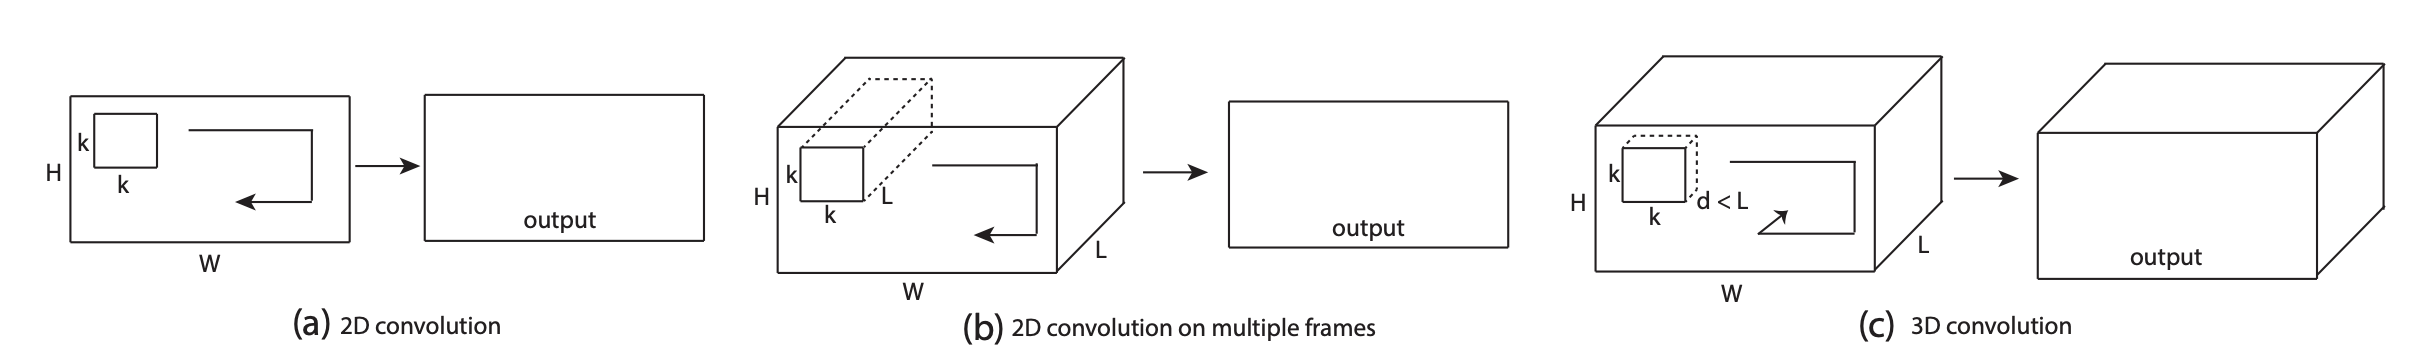
\includegraphics[width=\linewidth]{3dcnn.png}
    \caption{2D 和 3D 卷积示意图~\cite{tran2015c3d}。2D 卷积在图像或视频帧上运算得到特征图,而 3D 卷积可在视频序列上同时提取时空特征。}
    \label{fig:3dcnn}
\end{figure}

\subsection{视觉变换器}
随着Transformer在自然语言处理领域取得巨大成功,研究者们开始探索将其应用于计算机视觉任务。视觉变换器(Vision Transformer, ViT)是这一探索的代表性成果。不同于CNN基于局部感受野的特征提取方式,ViT将输入图像分割成固定大小的图像块(patches),并将这些图像块序列化后输入Transformer进行处理。通过自注意力机制,ViT能够建模图像块之间的全局依赖关系,为视觉特征提取提供了新的范式。

鉴于视觉 Transformer 在图像领域的成功,一些工作将其拓展到视频领域,提出了视频变换器(Video Transformer)。
典型的 Video Transformer 结构包括 时空分离(Spatiotemporal Separated) 和 时空联合(Joint Spatiotemporal) 两种策略。前者如 TimeSformer \cite{bertasius2021space},通过独立的时间和空间注意力进行计算,减少计算复杂度;后者如 ViViT \cite{arnab2021vivit},直接在 3D 令牌(Token)上施加全局注意力,以获得更强的时空建模能力。视频变换器在动作识别、视频理解等任务上已经展现出强大的性能。

% 建议在这里插入一张Video Transformer结构示意图
\begin{figure}[htbp]
    \centering
    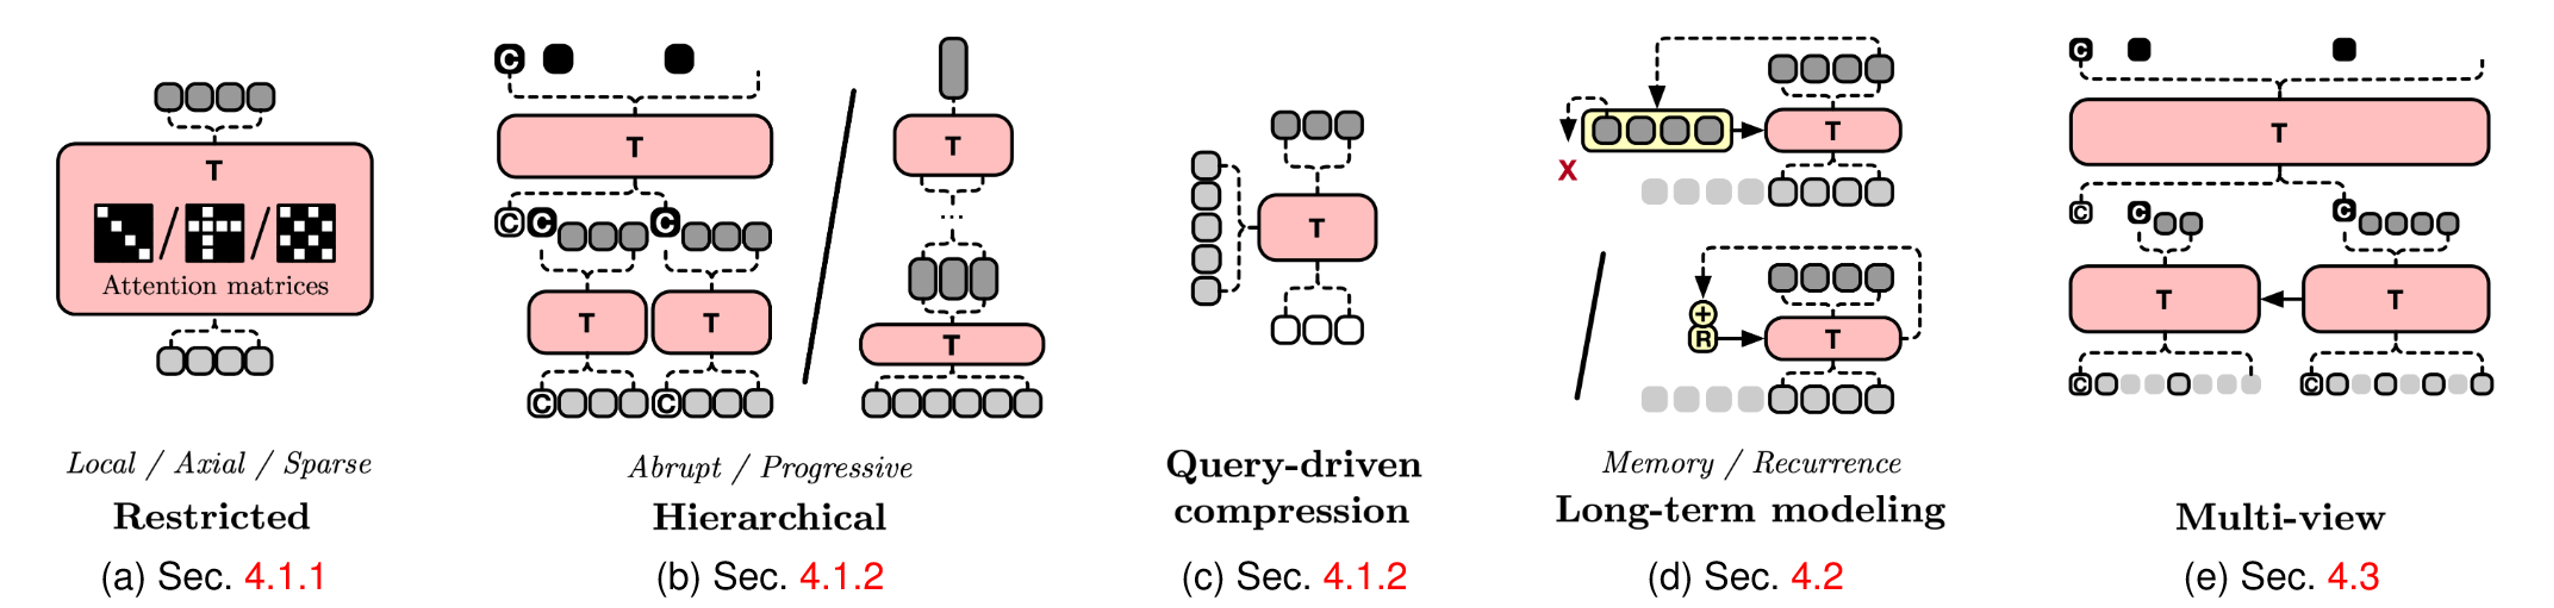
\includegraphics[width=\linewidth]{vt.png}
    \caption{Video Transformer 不同设计选择的可视化~\cite{selva2023video}。数据标记采用浅灰色(如果使用标记则采用黑色描边),而增强标记采用深灰色;白色标记是初始化的可学习标记;[CLS] 标记用“C”表示(增强后填充黑色)。从侧面流入 (T) 变压器的数据用于交叉注意。}
    \label{fig:vt}
\end{figure}

\section{生成模型基础}

\subsection{变分自编码器}

变分自编码器(VAE)\cite{kingma2013vae} 是一类通过概率建模实现数据生成的深度学习模型。
与传统自编码器不同,VAE 的核心思想是对潜在变量进行概率建模,学习数据的概率分布,而不是直接学习数据到数据的映射。这种基于概率的建模方式使得VAE能够生成多样化的样本,并且具有良好的插值性质。

VAE 假设观测数据由某个潜在变量生成,其生成过程可表示为 $p_{\theta}(\mathbf{x} \mid \mathbf{z})$,其中 $\mathbf{z}$ 服从某一先验分布(通常为标准正态分布)。然而,直接计算后验分布 $p_{\theta}(\mathbf{z} \mid \mathbf{x})$ 通常是不可行的,因此 VAE 采用变分推断,引入一个近似分布 $q_{\phi}(\mathbf{z} \mid \mathbf{x})$ 来进行估计。
模型的优化目标是最大化数据的对数似然,由于难以直接计算,通常转而最大化其证据下界(ELBO):
\begin{equation}
    \log p_{\theta}(\mathbf{x}) \geq \mathbb{E}_{q_{\phi}(\mathbf{z} \mid \mathbf{x})} \left[ \log p_{\theta}(\mathbf{x} \mid \mathbf{z}) \right] - D_{\mathrm{KL}} \left( q_{\phi}(\mathbf{z} \mid \mathbf{x}) \parallel p(\mathbf{z}) \right).
\end{equation}
其中,第一项鼓励模型在给定 $\mathbf{z}$ 的情况下能够准确重构数据,第二项则约束潜在变量的分布,使其接近先验分布,以保证生成的合理性。

在实际实现中,VAE 采用神经网络参数化编码器和解码器,其中编码器将输入数据映射为潜在变量的均值和方差,并通过重参数化技巧 $\mathbf{z} = \boldsymbol{\mu} + \boldsymbol{\sigma} \odot \boldsymbol{\epsilon}$(其中 $\boldsymbol{\epsilon} \sim \mathcal{N}(\mathbf{0}, \mathbf{I})$)实现可微分的采样。最终,通过梯度优化训练,使 VAE 既能够进行数据重构,又能生成高质量的新样本。

% 在训练过程中,VAE通过最大化数据的边际似然来优化模型参数。为了使优化过程可行,VAE引入了变分推断的思想,使用神经网络来近似后验分布。模型的训练目标包括重构误差和KL散度两部分,这种设计既保证了重构质量,又能够约束隐变量空间的结构。在本文手势生成任务中,VAE用于学习手势动作的低维表示,为后续的条件生成提供基础。

\subsection{扩散模型}
扩散模型(Diffusion Model)~\cite{ho2020ddpm} 是一类生成模型,通过逐步去噪的方式学习从噪声分布到数据分布的映射。该模型由前向(扩散)过程和反向(去噪)过程组成,其中前向过程逐步向数据添加噪声,而反向过程学习从噪声中逐步恢复数据分布,实现样本生成。
扩散模型的一个重要优势是其生成结果多样,生成质量高。通过精心设计的噪声调度,模型能够逐步学习数据分布的不同尺度特征。

% 建议在这里插入扩散模型原理示意图
% \begin{figure}[htbp]
%     \centering
%     % \includegraphics[width=0.8\linewidth]{diffusion.pdf}
%     \caption{扩散模型的前向和反向过程示意图}
%     \label{fig:diffusion}
% \end{figure}

\subsubsection{扩散模型的前向与反向过程}
\textbf{前向过程}通过在 $T$ 个时间步内逐步向数据样本 $\mathbf{x}_0 \sim q(\mathbf{x}_0)$ 添加高斯噪声,形成数据序列 $\{\mathbf{x}_t\}_{t=1}^{T}$,其定义如下:
\begin{equation}
    q(\mathbf{x}_t \mid \mathbf{x}_{t-1}) = \mathcal{N}(\mathbf{x}_t; \sqrt{1 - \beta_t} \mathbf{x}_{t-1}, \beta_t \mathbf{I}),
\end{equation}
其中,$\beta_t \in (0,1)$ 为控制噪声水平的方差调度参数。通过重参数化技巧,该分布可直接表示为 $\mathbf{x}_0$ 的函数:
\begin{equation}
    q(\mathbf{x}_t \mid \mathbf{x}_0) = \mathcal{N}(\mathbf{x}_t; \sqrt{\bar{\alpha}_t} \mathbf{x}_0, (1 - \bar{\alpha}_t) \mathbf{I}),
\end{equation}
其中 $\bar{\alpha}_t = \prod_{i=1}^{t} (1 - \beta_i)$。此公式允许从任意中间时间步高效采样。

\textbf{反向过程}旨在建模后验分布 $q(\mathbf{x}_{t-1} \mid \mathbf{x}_t)$,但该分布通常难以直接求解。为此,使用可学习的神经网络 $p_{\theta}$ 进行近似:
\begin{equation}
    p_{\theta}(\mathbf{x}_{t-1} \mid \mathbf{x}_t) = \mathcal{N}(\mathbf{x}_{t-1}; \boldsymbol{\mu}_{\theta}(\mathbf{x}_t, t), \Sigma_{\theta}(\mathbf{x}_t, t)).
\end{equation}
在大多数实现中,协方差 $\Sigma_{\theta}(\mathbf{x}_t, t)$ 可以固定或学习,而均值 $\boldsymbol{\mu}_{\theta}(\mathbf{x}_t, t)$ 通常由神经网络建模。

训练过程中,模型学习预测加入的噪声 $\boldsymbol{\epsilon}$,训练目标是最小化重建误差:
\begin{equation}
    \mathcal{L} = \mathbb{E}_{t,\mathbf{x}_0,\boldsymbol{\epsilon}}[\|\boldsymbol{\epsilon} - \boldsymbol{\epsilon}_\theta(\sqrt{\bar{\alpha}_t}\mathbf{x}_0 + \sqrt{1-\bar{\alpha}_t}\boldsymbol{\epsilon},t)\|_2^2]
\end{equation}
在推理阶段,模型通过从标准高斯分布 $\mathbf{x}_T \sim \mathcal{N}(\mathbf{0}, \mathbf{I})$ 逐步去噪,最终生成符合数据分布的样本。
通过这种设计,扩散模型能够在保证生成质量的同时,实现稳定的训练过程。


\subsubsection{条件扩散模型}
扩散模型通过在去噪过程中引入条件信息,可以实现对生成过程的精确控制。目前条件控制生成主要有两种范式:基于分类器引导的事后修改(Classifier-Guidance)~\cite{dhariwal2021diffusion}和无分类器引导的事前训练(Classifier-Free)~\cite{ho2022classifier}。

基于分类器引导的方法(Classifier-Guidance)首先训练一个无条件扩散模型,然后利用额外的分类器在推理阶段调整生成过程以实现条件控制。这种方法的优点是训练成本较低,可以复用已有的预训练模型;但其缺点是推理计算开销大,且对生成结果的细节控制能力有限。此外,分类器的质量也会直接影响生成效果。

无分类器引导的方法(Classifier-Free-Guidance)则直接在扩散模型的训练过程中加入条件信号,使模型能够在生成过程中自然地融入条件信息,而无需依赖显式的分类器。这种方法能够实现更精细的条件控制,生成质量也更有保障。但其主要缺点是需要较大的训练开销,对计算资源和训练数据的要求较高。在实际应用中,需要根据具体场景的资源约束和性能需求来选择合适的条件控制策略。

  % 国内外研究现状综述  
% !TeX root = ../thuthesis-example.tex

% \chapter{研究方法}
\chapter{基于多模态的动态手势识别算法}
\label{sec:GR}
针对手语教学中的动作评估挑战,本章对基于多模态的动态手势识别算法进行了研究。
为了解决动态手势识别中“信息冗余(Information Redundancy,IR)”和 “信息缺失(Information Absence,IA)”的问题,如图~\ref{fig:MDSI} 所示,本文提出了一种用于 RGB-D 手势识别的新型可插拔方法,称为多策略解耦和语义集成网络 (Multi-strategy Decoupling with Semantic Integration Network,MDSI)。所提出的可插拔式 MDSI 方法的总体框架如图 \ref{fig:MDSI} 所示。为了解决信息冗余 (IR) 问题,本文引入了多策略解耦网络 (Multi-strategy Decoupling Network,MDN),通过“姿势-运动”和“空间-时间-通道”解耦来强调不同尺度与不同维度的特征信息 (第~\ref{sec:MDN}节)。
为了解决信息缺失 (IA) 问题,本文提出了一个语义集成网络 (Semantic Integration Network,SIN),它有两个关键组件:语义滤波器 (Semantic Filter,SF) 和语义标签平滑 (Semantic Label Smoothing,SLS),以补充手势识别中缺失的信息 (第~\ref{sec:SIN}节)。
所提出的方法在 IsoGD 和 THU-READ 两个大规模基准数据集上取得了先进的识别性能,展现了其在实际应用中的潜力。
%应用
\begin{figure}[tb]
  \centering
  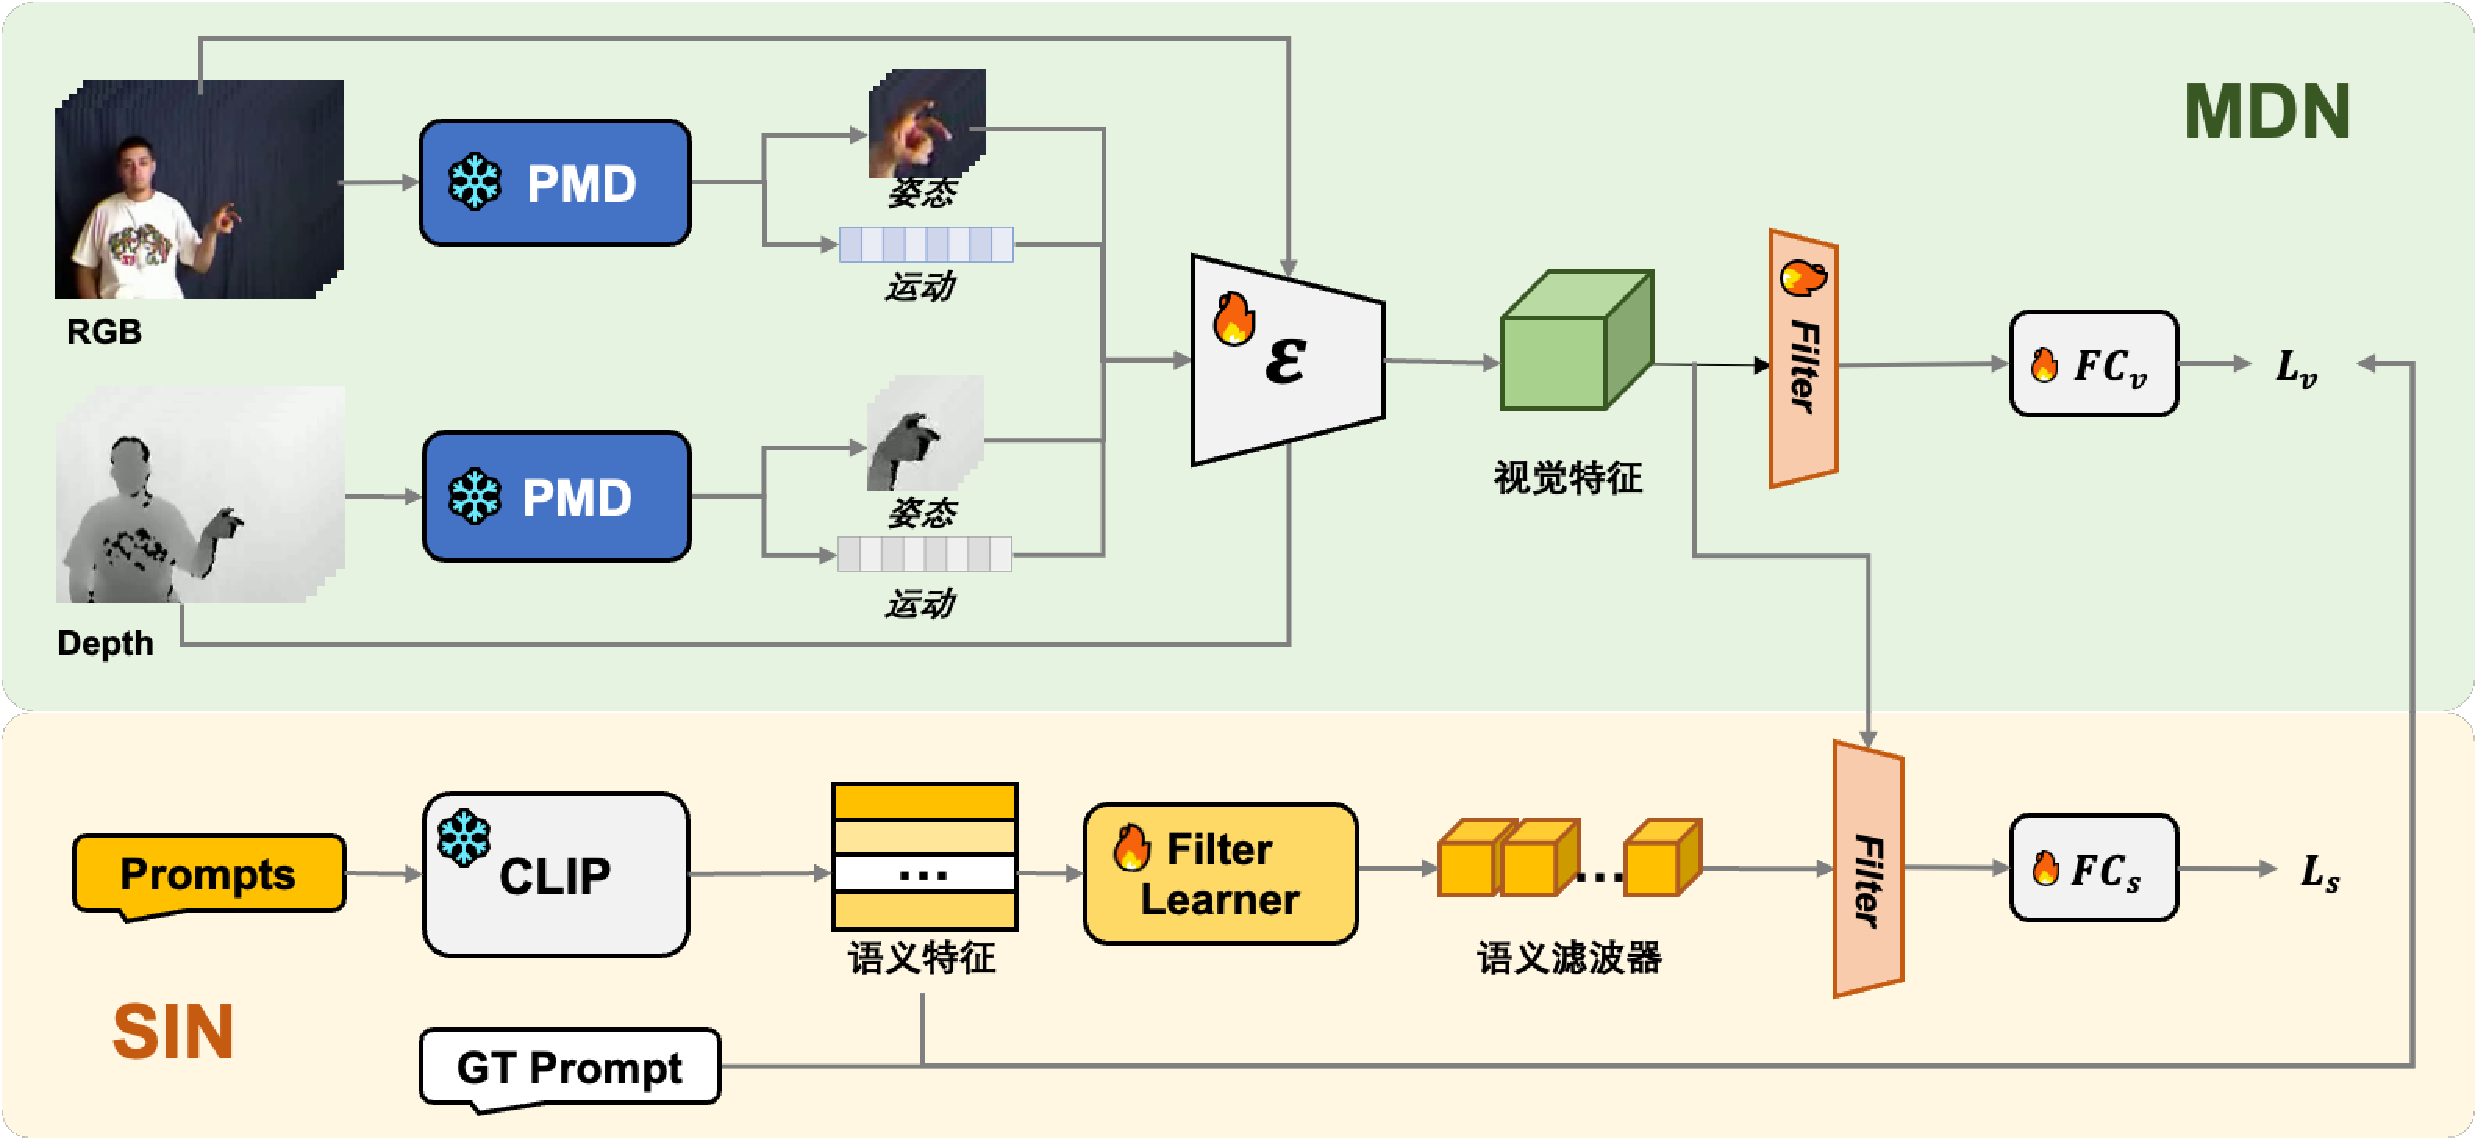
\includegraphics[width=\linewidth]{MDSI_v1.2.pdf}%framework.png}
  \caption{本文的可插入式多策略语义集成解耦 (MDSI) 框架概述。MDSI 可以无缝集成到基本编码器 $\varepsilon$ 中,从两个方面增强手势识别性能:
  i) 对于信息冗余,MDN (图~~\ref{fig:MDN}) 通过 PMD 和 STCD 强调不同维度和尺度的特征信息 (图~\ref{fig:handdecomp})。
  ii) 对于信息缺失,SIN 通过 SF 将自然语言建模与 SLS 一起集成到手势识别中 (图~\ref{fig:SIN})。}
  \label{fig:MDSI}
\end{figure}

\section{多策略手势特征解耦网络}
\label{sec:MDN}
\begin{figure}[tb]
  \centering
  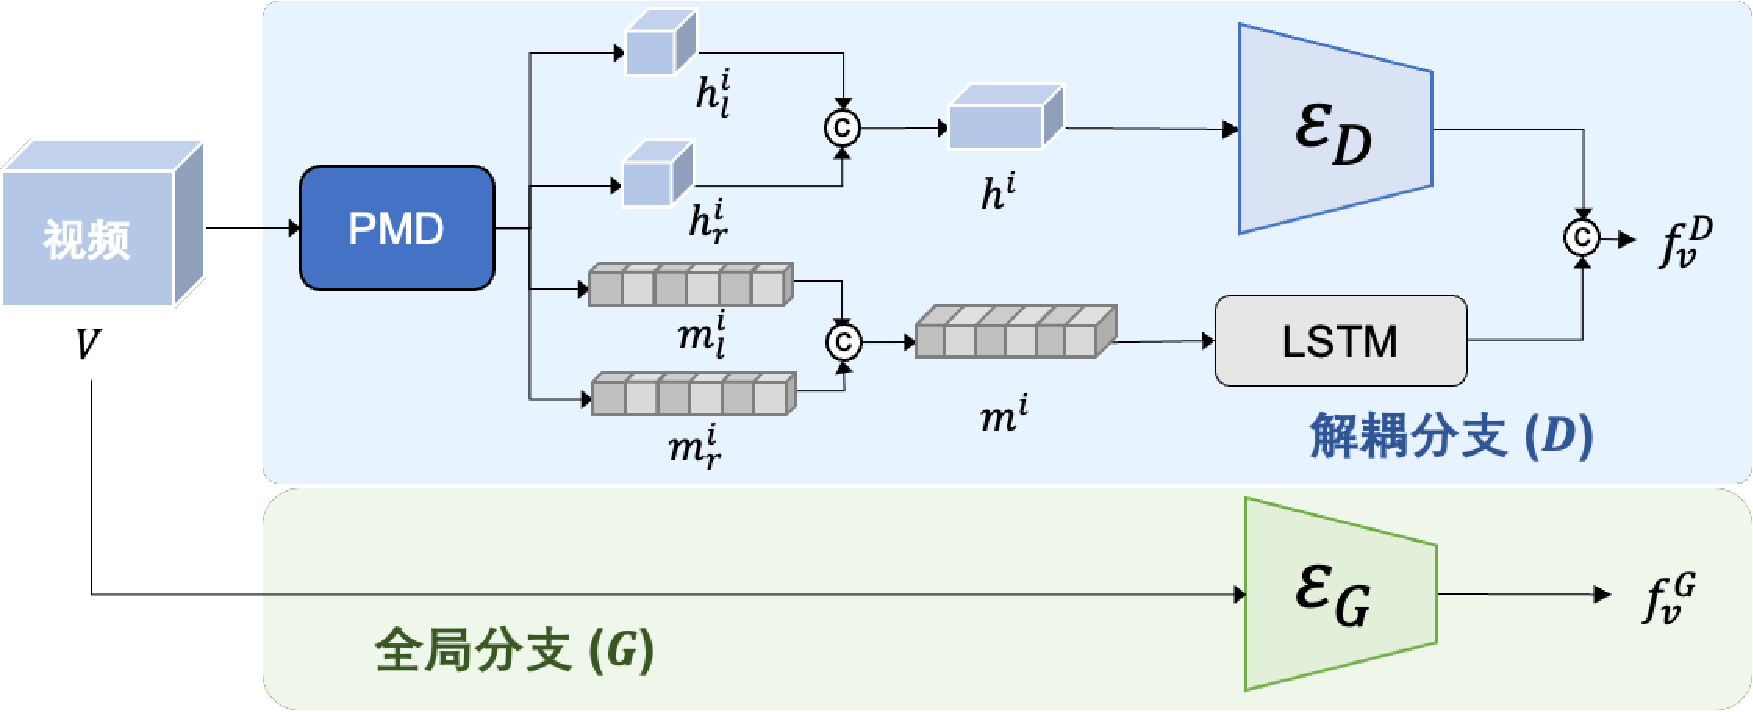
\includegraphics[width=0.8\linewidth]{MDN_v1.pdf}
    \caption{多策略解耦网络 (MDN)。MDN 配置为双分支视频编码器。i) 全局分支 ($\mathcal{G}$) 将原始视频 $\mathbf{V}$ 作为输入并对全局特征进行编码。ii) 解耦分支 ($\mathcal{D}$) 利用 PMD 模块同时捕获解耦的细粒度姿势 $\mathbf{h}$ 和粗粒度手部运动 $\mathbf{m}$。iii) STCD 模块插入编码器 $\varepsilon_{\mathcal{G}}$ 和 $\varepsilon_{\mathcal{D}}$ 的不同阶段,以执行与维度无关的解耦和注意。}
  \label{fig:MDN}
\end{figure}

在本节中,本文介绍了一种多策略解耦网络 (MDN),它配置为双分支架构,包括姿势-运动解耦模块 (PMD) 和空间-时间-通道解耦模块 (STCD)。
如图~\ref{fig:MDN} 所示,本文首先利用 PMD 将手势视频 $\mathbf{V}$ 解耦为细粒度姿势 $\mathbf{h}$ 和粗粒度运动 $\mathbf{m}$。原始视频 $\mathbf{V}$ 以及解耦结果 $\mathbf{(h, m)}$ 通常分别输入到 MDN 的全局分支 ($\mathcal{G}$) 和分解分支 ($\mathcal{D}$) 进行视觉时空特征提取。
此外,可插入 STCD 插入编码器 $\varepsilon_{\mathcal{G}}$ 和 $\varepsilon_{\mathcal{D}}$ 的各个阶段,以实现有效的与维度无关的解耦和注意。

\subsection{姿态-运动解耦(PMD)}
\label{sec:pose-motion}
\begin{figure}[tb]
\centering
\subcaptionbox{\label{fig:PMD}}
{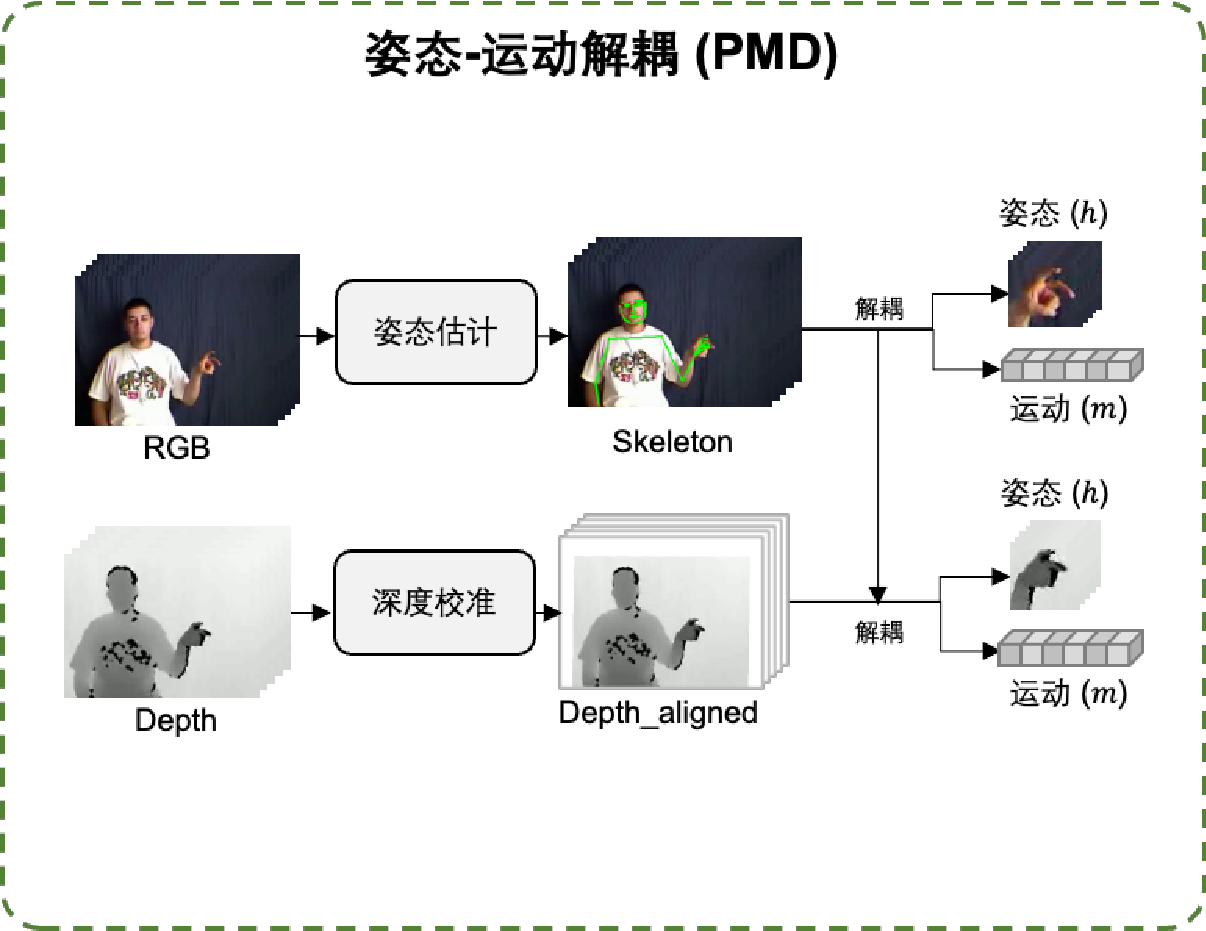
\includegraphics[width=0.44\linewidth]{PMD.pdf}}
\subcaptionbox{\label{fig:STCD}}
{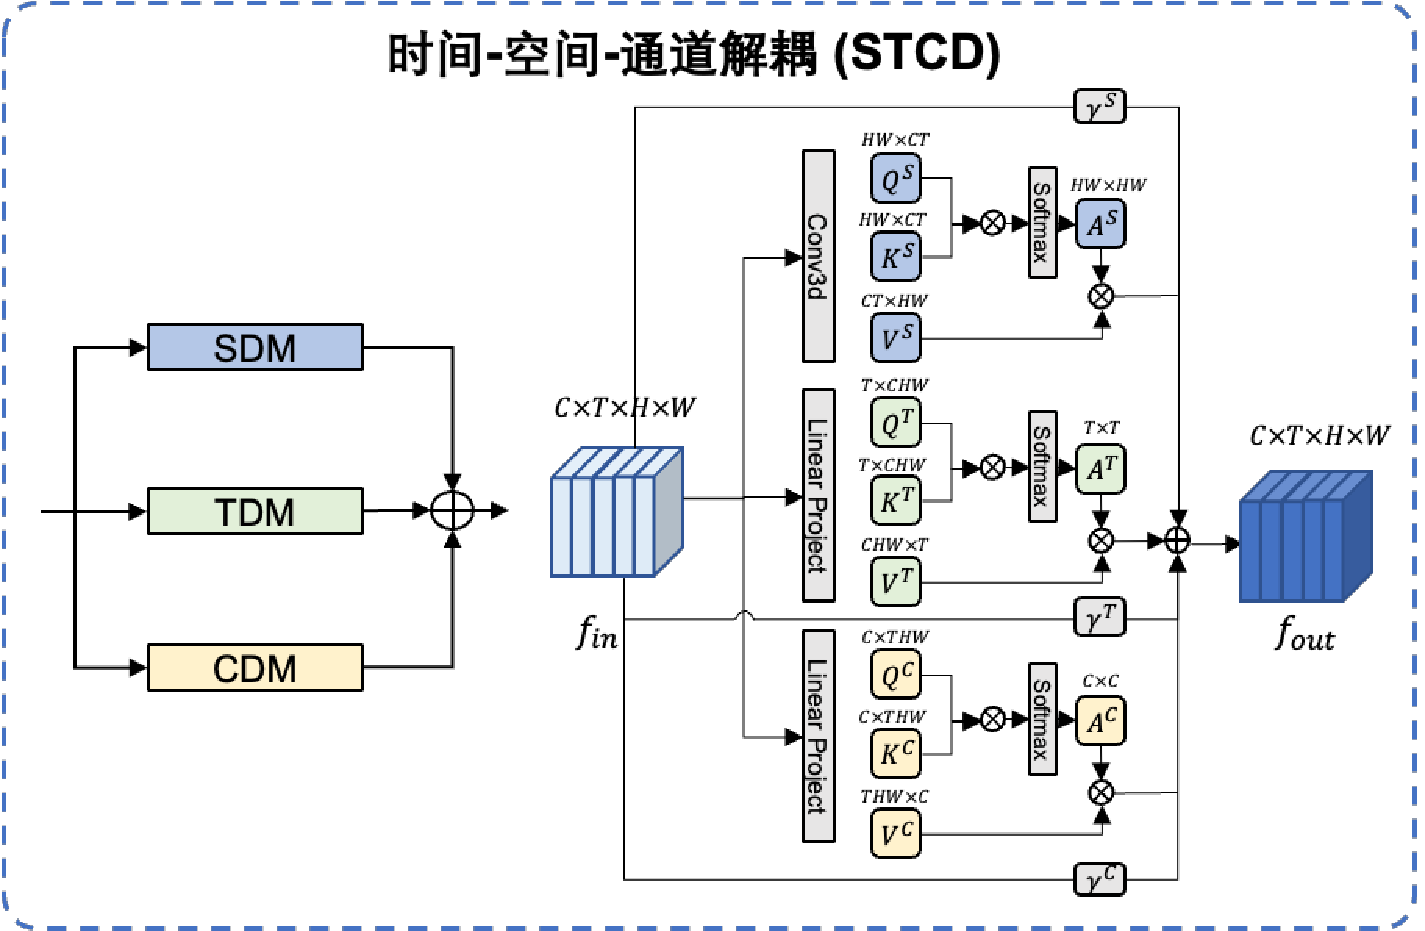
\includegraphics[width=0.52\linewidth]{STCDv1 .pdf}}
\caption{多策略解耦管道。 (a) 姿势-运动解耦 (PMD),(b) 空间-时间-通道解耦 (STCD)。}
\label{fig:handdecomp}
\end{figure}

如图~\ref{fig:PMD}所示,PMD 主要包括三个阶段:i) 姿势估计、ii) 深度校准和 iii) 姿势-运动解耦。
对于 RGB 数据,本文首先使用在 COCO-WholeBody 数据集 \cite{jin2020whole} 上预训练的姿势估计器 HRNet \cite{sun2019deep} 来提取并保存每帧 2D 身体骨架\footnote{请注意,姿势估计器在训练期间处于冻结状态,确保它不会引入任何额外的计算成本。此外,使用手部检测器检测和分割手部是领域内的常见做法 \cite{AVOLA2022108762,zhou2021regional,chen2022multi},这是一个完全公平的设置。}。
对于深度数据,本文提前进行视频校准以确保配准 \cite{liu2017continuous}。
具体来说,对于 IsoGD 数据集 \cite{wan2016chalearn},本文利用 Liu 等人提供的对齐深度视频数据 \cite{liu2017continuous},并进一步调整 Narayana 等人提供的深度数据映射 \cite{narayana2018focus},使用以下变换:$D'=\frac{D-7}{0.93}-14$。
对于 THU-READ 数据集,深度数据已提前校准。
对齐良好的深度数据可以采用从 RGB 视频中提取的相同骨架进行后续操作。

本文利用提取的骨架数据将原始视频 $\mathbf{V}$ 分解为手部姿势 $\mathbf{h}$ 和手部运动 $\mathbf{m}$。
首先,给定第 $i$ 帧的骨架数据 ($i \in 0, 1, ..., T$),本文分别过滤每只手的 22 个关键点并描绘出最小手部边界框。
随后,裁剪缩放后的边界框(比例=1.2)以获得表示细粒度姿势 $\mathbf{h}^{i}$ 的裁剪手部图像。为了公式化粗粒度运动向量$\mathbf{m}^{i} \in \mathbb{R}^{8}$,本文将边界框的 8 个位置属性堆叠如下:$\mathbf{m}^{i} = \left[e^{i}, x^{i}_{min}, y^{i}_{min}, x^{i}_{max}, y^{i}_{max}, w^{i}, h^{i}, r^{i}\right]^{\top}$,其中 $e^{i} \in \{0, 1\}$ 表示相应的手是否出现在第 $i$ 帧,$\{x^{i}_{min}, y^{i}_{min}\}$ 和 $\{x^{i}_{max}, y^{i}_{max}\}$ 为边界框左上角和右下角顶点的坐标,$w^{i}, h^{i}$ 分别对应宽和高,$r^{i}=w^{i}/h^{i}$ 表示长宽比。
为了区分左右手,上述操作分别在每只手上独立执行,然后连接起来,得到最终的解耦特征:$\mathbf{h}^{i} = \left[\mathbf{h}^{i}_l, \mathbf{h}^{i}_r\right]$,$\mathbf{m}^{i} = \left[\mathbf{m}^{i}_l, \mathbf{m}^{i}_r\right]$。
具体来说,$\mathbf{h}$ 和 $\mathbf{m}$ 分别在宽度方向和通道方向连接。

此外,为了减轻姿势估计不准确的影响,本文设计了一个 \emph{分割验证机制}:检测到的关键点置信度低且关键点数量较少的骨架被标记为错误检测,并且相应的姿势特征 $\mathbf{h}^{i}$ 被分配零值。%\textcolor{red}{更多详细信息请参阅 \ref{sec:appendix_pmd}。}

\subsection{空间-时间-通道解耦 (STCD)}
\label{sec:STCD}
鉴于手势识别中存在紧密耦合的时空冗余\cite{zhou2023unified},本文引入了 STCD(图 ~\ref{fig:STCD}),它配置了三个包含注意机制的独立于维度的模块:i) 空间解耦模块 (\textbf{SDM})、ii) 时间解耦模块 (\textbf{TDM}) 和 iii) 通道解耦模块 (\textbf{CDM})。
以$\varepsilon$中提取的输入中间特征图$\mathbf{f}_{in}\in \mathbb{R}^{C\times T\times H\times W}$作为输入,该框架帮助网络有效滤除各个维度上的冗余信息,输出优化的特征图$\mathbf{f}_{out}\in \mathbb{R}^{C\times T\times H\times W}$,从而帮助训练。

以 SDM 为例,其目的是识别每帧手势特征中的关键空间区域。首先,给定 $\mathbf{f}_{in}$,本文使用 Conv3d 来导出查询、键和值特征,分别表示为 $\mathbf{Q}^{\mathcal{S}}$、$\mathbf{K}^{\mathcal{S}}$ 和 $\mathbf{V}^{\mathcal{S}}$。
本文合并时间和通道维度以获得 \emph{空间} 查询、键和值向量:$\mathbf{q}^{\mathcal{S}}\in \mathbb{R}^{HW\times CT}$、$\mathbf{k}^{\mathcal{S}}\in \mathbb{R}^{HW\times CT}$、$\mathbf{v}^{\mathcal{S}}\in \mathbb{R}^{CT\times HW}$。
然后,利用 $\mathbf{q}^{\mathcal{S}}$ 和 $\mathbf{k}^{\mathcal{S}}$ 计算注意矩阵 $\mathbf{A}^{\mathcal{S}}\in \mathbb{R}^{HW\times HW}$,如下所示:

\begin{equation}
\mathbf{A}^{\mathcal{S}} = \text{softmax}\left(\mathbf{q}^{\mathcal{S}}\left(\mathbf{k}^{\mathcal{S}}\right)^{\top}\right).
\end{equation}
随后,空间注意力向量 $\mathbf{f}^{\mathcal{S}}\in \mathbb{R}^{CT\times HW}$ 可以通过以下公式计算:
\begin{equation}
\mathbf{f}^{\mathcal{S}} = \mathbf{v}^{\mathcal{S}} \mathbf{A}^{\mathcal{S}}.
\end{equation}
恢复时间和通道维度以获得空间注意特征图$\mathbf{f}'^{\mathcal{S}}\in \mathbb{R}^{C\times T\times H\times W}$。
此外,为了促进网络收敛并调节网络注意力水平,本文引入了可学习的残差连接。最终的空间优化特征$\mathbf{f}_{out}^{\mathcal{S}}$可以按如下方式计算:$\mathbf{f}_{out}^{\mathcal{S}} = \gamma^{\mathcal{S}} \mathbf{f}'^{\mathcal{S}} + \mathbf{f}_{in}$,
其中$\gamma^{\mathcal{S}}$是SDM的可学习残差权重。

TDM 和 CDM 分别关注手势特征中的关键帧和通道,其操作与 SDM 类似。
此外,STCD 的结果输出被表达为三个解耦模块输出的聚合。
具体而言,本文设计了一个并行范式 (图 ~\ref{fig:STCD})
STCD 的结果输出 ${f}_{out}$ 可以表示如下:$\mathbf{f}_{out} = \mathbf{f}_{out}^{\mathcal{S}} + \mathbf{f}_{out}^{\mathcal{T}} + \mathbf{f}_{out}^{\mathcal{C}}$。

\subsection{双分支视频编码器}
\label{sec:DBVE}
如图~\ref{fig:MDN}所示,MDN 配置有两个分支:i) \emph{全局分支} ($\mathcal{G}$) 将原始视频 $\mathbf{V}$ 作为特征提取和识别的输入;ii) \emph{解耦分支} ($\mathcal{D}$) 利用解耦后的特征 $\mathbf{(h, m)}$ 作为输入,同时捕获细粒度的手势姿势变化和粗粒度的手部运动。
本文为每个分支配置一个视频编码器 $\varepsilon$。
此外,本文在 $\mathcal{D}$ 分支中引入了一个长短期记忆 (LSTM) 模型,用于运动建模(图~\ref{fig:MDN})。
特征提取过程可以表述如下:
\begin{equation}
\label{eq:fv}
\begin{aligned}
  \mathbf{f}_{v}^{\mathcal{G}} &= \Phi_{\mathcal{G}}(\mathbf{V}), \\
  \mathbf{f}_{v}^{\mathcal{D}} &= \Phi_{\mathcal{D}}(\mathbf{h}, \mathbf{m}).
\end{aligned}
\end{equation}
其中$\Phi_{\mathcal{G}}$表示$\mathcal{G}$分支网络,$\Phi_{\mathcal{D}}$表示$\mathcal{D}$分支网络。
得到的视觉特征$\mathbf{f}_{v}^{\mathcal{G}}, \mathbf{f}_{v}^{\mathcal{D}}$将分别输入到下面的SIN网络中进行语义集成。

\begin{figure}[tb]
\centering
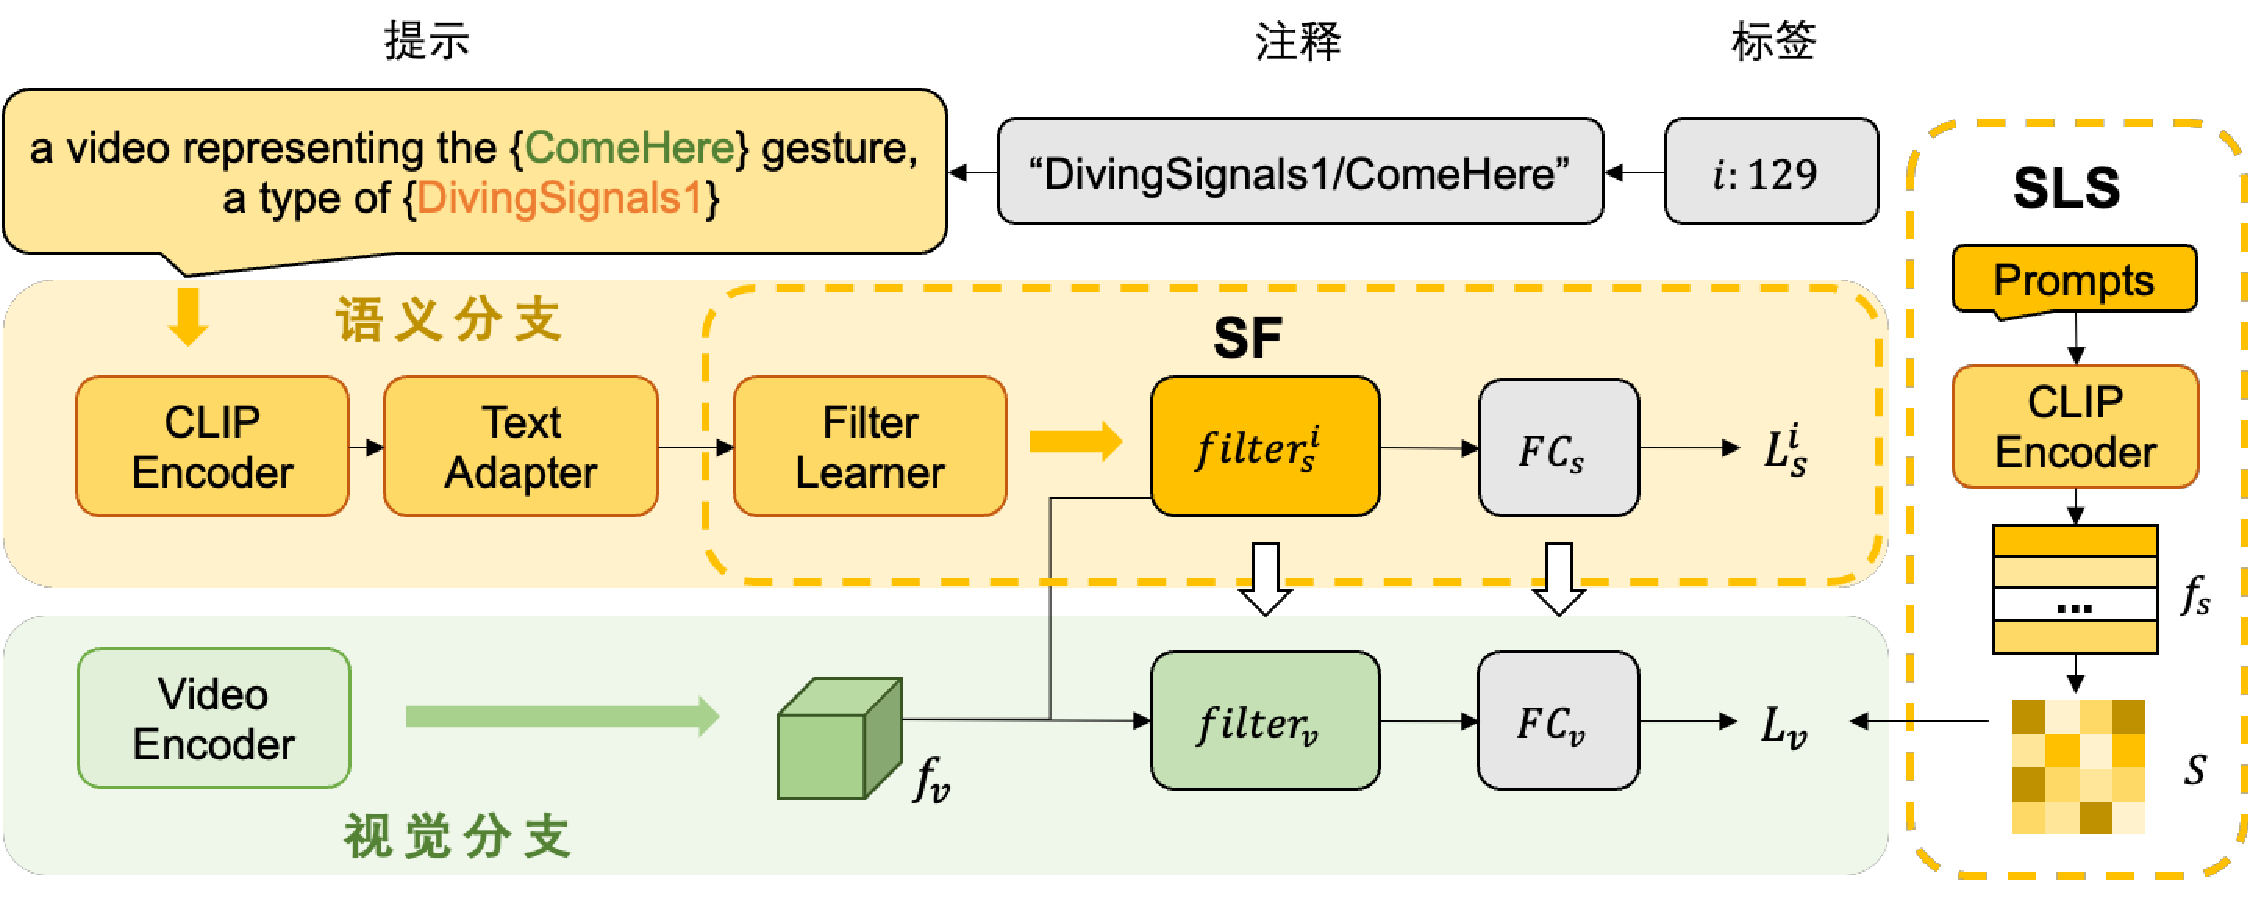
\includegraphics[width=1.0\linewidth]{SIGRv1 .pdf}
\caption{语义集成网络 (SIN) 。通过引入语义滤波器 (SF) 和语义标签平滑 (SLS),以促进语义知识整合。 }
\label{fig:SIN}
\end{figure}
\section{多模态手势语义集成网络}
\label{sec:SIN}
手势识别中的信息缺失挑战(第~\ref{sec:intro}节)激励本文结合自然语义信息作为指导。
所提出的语义集成网络 (SIN)(如图~\ref{fig:SIN} 所示)由两个分支组成:i) \emph{semantic} 分支,以语义嵌入和语义滤波器 (SF) 为特色;ii) \emph{vision} 分支,以语义标签平滑 (SLS) 为辅助。

\subsection{语义嵌入}
如图~\ref{fig:SIN}所示,鉴于手势数据集 \cite{wan2020chalearn,tang2017action,molchanov2016online} 通常使用类索引作为标签,本文首先生成与手势标签相对应的语义提示。具体来说,本文编译语义注释并设计提示(prompt),以强调每个手势数据集的独特特征。
然后,本文利用预训练的 CLIP 的文本编码器 \cite{radford2021learning} 和适配器 \cite{gao2024clip} 生成和细化深度语义嵌入 $\mathbf{f}_{s}\in \mathbb{R}^{N\times 1024}$($N$ 表示类数)。%\textcolor{red}{有关进一步的实施细节,请参阅 \ref{sec:appendix_se}。}

\subsection{语义滤波器 (SF)}
从动态卷积技术中汲取灵感~\cite{yang2019condconv,chen2020dynamic},本文引入了语义滤波器 (SF),用于通过卷积混合多模态特征。%(有关更多详细信息,请参阅 \ref{sec:appendix_SF})。

本文引入一个线性\emph{Filter Learner}(图~\ref{fig:SIN})来导出语义滤波器。
设语义滤波器的数量为$n$,以相应的$n$个语义嵌入$\mathbf{f}_{s} \in \mathbb{R}^{n\times 1024}$为输入,通过线性映射输出语义滤波器参数$\mathbf{f'}_{s}\in \mathbb{R}^{n\times N_p}$,然后将这些参数重塑为$n$个语义滤波器$\boldsymbol{\Theta}_{s}\in \mathbb{R}^{n\times c\times k^{d_k}}$,其中每个滤波器$\boldsymbol{\Theta}_{s}^i$代表一个卷积核。
第 $i$ 个滤波器 $\boldsymbol{\Theta}_{s}^i$ 的参数数量定义为:$N_p=c\times k^{d_k}$,其中 $c$ 表示视觉特征 $\mathbf{f}_{v}$ 的输入通道(式\eqref{eq:fv}),$k$ 表示滤波器核大小(经验上设置为 3),$d_k$ 表示卷积维数(例如,对于 3d 卷积核,设置 $d_k=3$)。

随后,本文将每个 $\boldsymbol{\Theta}_{s}^i$(对应第 $a$ 个手势类别)作为过滤核,将视觉特征 $\mathbf{f}_{v}$(对应第 $b$ 个手势类别)作为输入,执行深度卷积。得到的每个混合语义特征 $\mathbf{f}_{SF}^i$ 可以表示为:
\begin{equation}
\mathbf{f}_{SF}^{i} = \text{Convolution}\left(\mathbf{f}_{v}, \boldsymbol{\Theta}_{s}^i\right),\quad i \in 1\dots n. \\
\end{equation}
这些混合语义特征被进一步激活和扁平化,通过全连接(FC)层生成语义分支识别结果。

为了监督语义分支的优化,本文将每个语义标签 $a$ 与样本视觉标签 $b$ 混合 \cite{zuo2023natural}。
具体来说,语义分支的混合标签 $\mathbf{y}_{SF}^i \in \mathbb{R}^N$ 可以表示为:
\begin{equation}
y_{SF}^i[k] = \begin{cases}
1 & \text{如果 } k = a = b,\\
0.5 & \text{如果 } k = a \text{或 } k = b, a\neq b,\\
0 & \text{否则,}
\end{cases}
\end{equation}
其中 $y_{SF}^i[k]$ 表示 $\mathbf{y}_{SF}^i$ 的第 $k$ 个条目。
本文利用交叉熵损失来优化语义滤波器:
\begin{equation}
L_{s}^i = -\frac{1}{N}\sum_{k=1}^{N}{{y}_{SF}^i[k] \log\left(\hat{y}^i[k]\right)},
\end{equation}
同样,本文根据选定的 $n$ 个语义滤波器形成 $n$ 个混合标签,并获得相应的 $n$ 个语义预测。整体语义损失 $L_{s}$ 是 $n$ 个交叉熵损失的平均值:$L_{s} = \frac{1}{n}\sum_{i=1}^{n}{L_{s}^i}$。

如图~\ref{fig:SIN} 所示,为了捕获 SF 中嵌入的语义知识以进行 \textbf{推理},本文引入了一个与视觉滤波器 $\boldsymbol{\Theta}_{v}$ 类似的卷积核,遵循本文的视觉网络 MDN,并将语义分支的知识集成到视觉分支中。
具体而言,$\boldsymbol{\Theta}_{v}$ 和 $FC_{v}$ 分别通过其参数的加权和以及相应的 $\boldsymbol{\Theta}_{s}$ 和 $FC_{s}$ 的参数进行更新。
% 有关更多实施细节,请参阅 \ref{sec:appendix_hp}。

\subsection{语义标签平滑(SLS)}
与普通标签平滑 \cite{he2019bag} 相比,本文利用手势的语义相似性来生成有偏平滑标签,从而增强视觉分支识别视觉相似手势的能力。
具体来说,本文首先通过 CLIP 的文本编码器获取语义嵌入 $\mathbf{f}_{s} \in \mathbb{R}^{N\times 1024}$,然后使用余弦相似度 \cite{zuo2023natural} 构建提示相似度表 $\mathbf{S}$:$\mathbf{S} = \|\mathbf{f}_{s}\|_2\|\mathbf{f}_{s}\|_2^{\top} \in \mathbb{R}^{N\times N}$。
%
对于第 $b$ 个手势类别的训练样本,建议的平滑标签 $\mathbf{y}_{SLS}$ 可以表示为:
\begin{equation}
y_{SLS}[k] = \begin{cases}
1 - \sigma & \text{如果 } k = b,\\
\sigma \times \text{softmax}\left(S[b][k]/\tau\right) & \text{否则},
\end{cases}
\end{equation}
其中 $\sigma=0.2$,$\tau=0.5$。
类似地,交叉熵用于计算视觉分支损失:
\begin{equation}
L_{v} = -\frac{1}{N}\sum_{k=1}^{N}{y_{SLS}[k]\log\left(\hat{y}[k]\right)}. %SLS(\hat{y}_{vision},y)
\end{equation}

\subsection{整体损失}
整体损失是 $L_{s}$ 和 $L_{v}$ 的加权和:
\begin{equation}
Loss = w_{s} \times L_{s} + w_{v} \times L_{v}.
\label{eq:overall_loss}
\end{equation}
%
请注意,本文仅将 SIN 网络应用于每个全局视觉特征 $f_v^G$ (式~\eqref{eq:fv}),以确保视觉特征和语义特征之间交互的完整性。
最后,本文采用常用的分数融合方法来结合每个分支和模态的预测。

\section{实验结果与分析}
\label{sec:GR_EXP}
\subsection{实验设置}
\subsubsection{数据集}
本文在两个公共 RGB-D 手势数据集上评估了本文的方法:IsoGD \cite{wan2016chalearn} 和 THU-READ \cite{tang2017action}。它们都已被广泛使用,并且包含具有挑战性的场景。
IsoGD 数据集 \cite{wan2016chalearn} 收录了 47933 段 RGB-D 手势视频,由 21 位受试者完成 249 类手势动作。本文图 ~\ref{fig:samples} 展示了该数据集的示例样本。
此数据集中样本的背景多样性和手势相似性使其成为评估本文的方法对信息冗余 (IR) 和信息缺失 (IA) 影响的良好基准。
THU-READ 数据集 \cite{tang2017action} 包含 1920 个 RGB-D 自我中心手势视频,包含 8 个受试者执行的 40 个不同动作,由于细微的类内差异和背景噪音,这仍然具有挑战性。
为了进行评估,本文采用提供的留一法交叉验证协议 \cite{li2021trear}。

% 进一步地,本文利用奥比中光机器人平台(第~\ref{sec:robot}节)构建了自采数据集,并基于此评估了本文的方法。如图~\ref{fig:aobi_sample}所示,本文共采集了12类手势数据,每类包含25个样本。

% \begin{figure}
%   \centering
%   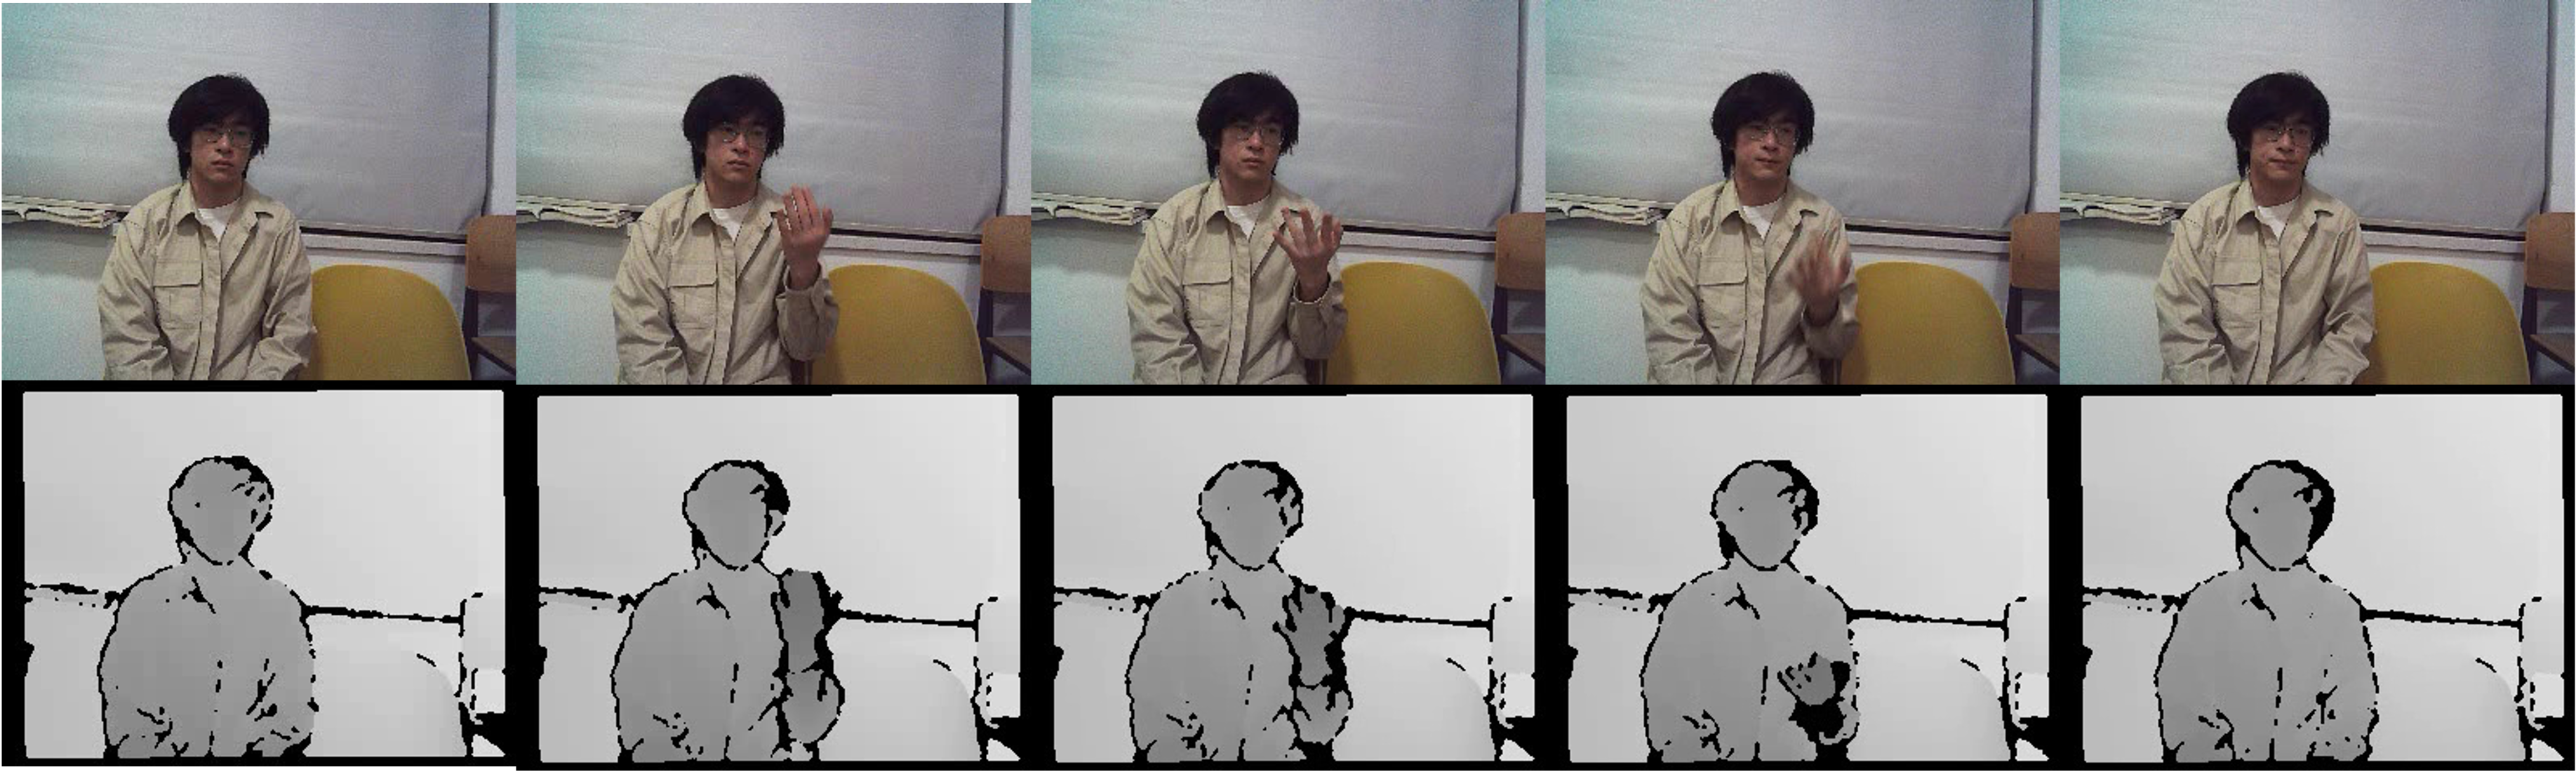
\includegraphics[width=0.8\linewidth]{aobi_sample.png}
%   % \caption*{}
%   \caption{机器人平台自采数据集样本示例}
%   \label{fig:aobi_sample}
% \end{figure}


\subsubsection{编码器骨干}
\label{sec:encoder_backbone}
本文实现了两个版本的 MDSI: \emph{MDSI-CNN} 和 \emph{MDSI-Transformer},分别将本文的可插拔方法集成到基于 CNN 的视频编码器 \cite{zhu2018continuous} 和基于 Transformer 的视频编码器 \cite{zhou2022decoupling} 中。这突出了 MDSI 的可插拔特性,使其能够集成到不同的编码器架构中。本文将这两个版本与最先进的方法进行比较,以验证本文的方法。

\subsubsection{实现细节}
\label{sec:implementation}
本文使用 Adam 作为优化器。
训练时,每个视频随机抽取32帧连续序列。原始输入序列随机裁剪至224 $\times$ 224像素,解耦的
手部序列调整至112 $\times$ 112像素。
数据增强包括空间裁剪、旋转、翻转和 Shufflemix+ \cite{zhou2023unified}。
与~\cite{yu2021searching,zhou2021regional,zhou2022decoupling,zhou2023unified} 类似,本文所有的实验都是在 20BN Jester V1 数据集上进行预训练的~\cite{materzynska2019jester}。
在推理过程中,输入序列被中心裁剪为 224 × 224。
本文根据视觉特征形状分别将 MDSI-CNN 和 MDSI-Transformer 的 SF 中的卷积维度 $d_k$ 设置为 3 和 1。
除非另有说明,所有消融研究均在 IsoGD 数据集的 RGB 数据上进行。
% 有关更多实施细节,请参阅 \ref{sec:appendix_hp}。

% \renewcommand{\arraystretch}{0.75}
% \setlength{\abovecaptionskip}{4pt}
% \setlength{\belowcaptionskip}{4pt}
% \setlength{\textfloatsep}{8pt}
\begin{table*}[htbp] %[!ht]
% \small
  \caption{与 IsoGD 数据集上最先进的方法的性能比较。最佳和第二佳方法通过 \textbf{加粗} 和 \underline{下划线}标注。}
    \centering
    \begin{tabular}{cccc}
    \toprule 
        {Modality} & {Backbone} &  {Methods}& {Accuracy(\%)} \\
     \midrule
        \multirow{9}*{RGB}& \multirow{5}*{CNN}  & ConvLSTMForGR~\cite{zhu2019redundancy}  & 57.42 \\ 
        ~&~& NAS~\cite{yu2021searching}  &  58.88 \\ 
        ~&~& RAAR3DNet~\cite{zhou2021regional} &  62.66 \\ 
        ~&~& MSA-3D~\cite{chen2022multi} & \underline{62.73} \\ 
        ~&~& \textbf{Ours} & \textbf{72.79} \\ 
        \cmidrule(lr){2-4}
        ~& \multirow{4}*{Transformer} & Decouple+Recouple~\cite{zhou2022decoupling} & 60.87 \\ 
        ~&~& MFST-Large~\cite{ma2023multi} & 61.26 \\ 
        ~&~& UMDR (32 frame)~\cite{zhou2023unified} & \underline{63.68} \\ 
        ~&~& \textbf{Ours} & \textbf{68.32} \\ 
     \midrule
        \multirow{9}*{Depth}& \multirow{5}*{CNN}  & ConvLSTMForGR~\cite{zhu2019redundancy} & 54.18 \\ 
        ~&~& NAS~\cite{yu2021searching} & 55.68 \\ 
        ~&~& RAAR3DNet~\cite{zhou2021regional} & 60.66 \\ 
        ~&~& MSA-3D~\cite{chen2022multi} & \underline{61.72} \\ 
        ~&~& \textbf{Ours} & \textbf{65.99} \\ 
        \cmidrule(lr){2-4}
        ~& \multirow{4}*{Transformer} & Decouple+Recouple~\cite{zhou2022decoupling}& 60.17 \\ 
        ~&~& MFST-Large~\cite{ma2023multi}& 61.29 \\ 
        ~&~& UMDR (32 frame)~\cite{zhou2023unified}& \underline{64.62} \\ 
        ~&~& \textbf{Ours} & \textbf{68.00} \\ 
     \midrule
        \multirow{9}*{RGB-D}& \multirow{5}*{CNN}  &ConvLSTMForGR~\cite{zhu2019redundancy}& 61.05 \\ 
        ~&~& NAS~\cite{yu2021searching}& 65.54 \\ 
        ~&~& RAAR3DNet~\cite{zhou2021regional}& 66.62 \\ 
        ~&~& MSA-3D~\cite{chen2022multi}& \underline{68.15} \\
        ~&~& \textbf{Ours}& \textbf{75.09} \\ 
        \cmidrule(lr){2-4}
        ~& \multirow{4}*{Transformer} & Decouple+Recouple~\cite{zhou2022decoupling}& 66.79 \\ 
        ~&~& MFST-Large~\cite{ma2023multi}& 68.47 \\ 
        ~&~& UMDR (32 frame)~\cite{zhou2023unified}& \underline{72.61} \\ 
        ~&~& \textbf{Ours}& \textbf{74.73} \\ 
  \bottomrule
    \end{tabular}
  \label{tab:Iso SOTA}
\end{table*}

\begin{table*}[htbp] %[!ht]
% \small
  \caption{与 THU-READ 数据集上最先进的方法的性能比较。最佳和第二佳方法通过 \textbf{加粗} 和 \underline{下划线}标注。}
    \centering
    \begin{tabular}{cccc}
    \toprule 
        {Modality} & {Backbone} & {Methods} &  {Accuracy(\%)} \\
     \midrule
        \multirow{9}*{RGB}& \multirow{5}*{CNN} & VGG~\cite{simonyan2014very} &41.90 \\ 
        ~&~&SlowFast~\cite{feichtenhofer2019slowfast}& 69.58 \\ 
        ~&~&NAS~\cite{yu2021searching}& 71.25 \\ 
        ~&~&TSN~\cite{wang2016temporal}& \underline{73.85} \\ 
        ~&~&\textbf{Ours}& \textbf{78.34} \\ 
        \cmidrule(lr){2-4}
        ~& \multirow{4}*{Transformer} &Trear~\cite{li2021trear} & 80.42 \\ 
        ~&~&Decouple+Recouple~\cite{zhou2022decoupling} & 81.25 \\ 
        ~&~&UMDR (32 frame)~\cite{zhou2023unified} & \underline{82.50} \\ 
        ~&~&\textbf{Ours} & \textbf{85.30}\\
     \midrule
        \multirow{7}*{Depth}& \multirow{3}*{CNN} &VGG~\cite{simonyan2014very} &34.06 \\ 
        ~&~&TSN~\cite{wang2016temporal} &\underline{65.00} \\ 
        ~&~&\textbf{Ours} & \textbf{65.94} \\ 
        \cmidrule(lr){2-4}
        ~& \multirow{4}*{Transformer} &Trear~\cite{li2021trear} & 76.04 \\ 
        ~&~&Decouple+Recouple~\cite{zhou2022decoupling} &\underline{77.92}  \\ 
        ~&~&UMDR (32 frame)~\cite{zhou2023unified} &\textbf{79.59} \\ 
        ~&~&\textbf{Ours} & 74.87\\
     \midrule
        \multirow{7}*{RGB-D}& \multirow{3}*{CNN} & SlowFast~\cite{feichtenhofer2019slowfast} & 76.25 \\ 
        ~&~&NAS~\cite{yu2021searching} & \underline{78.38} \\ 
        ~&~&\textbf{Ours} & \textbf{82.71} \\ 
        \cmidrule(lr){2-4}
        ~& \multirow{4}*{Transformer} &Trear~\cite{li2021trear} & 84.90 \\ 
        ~&~&Decouple+Recouple~\cite{zhou2022decoupling} &87.04  \\ 
        ~&~&UMDR (32 frame)~\cite{zhou2023unified} &\underline{88.09} \\ 
        ~&~&\textbf{Ours} & \textbf{89.36} \\
  \bottomrule
    \end{tabular}
  \label{tab:THU SOTA}
\end{table*}

\begin{table*}
% \small
    \centering
  \caption{MDN 各个子分支的性能比较。“Trans.”表示 Transformer。}
  \begin{tabular}{cc@{\hspace{3pt}}c@{\hspace{3pt}}c@{\hspace{3pt}}ccc}
    \toprule
       \multirow{2}*{Branches} & \multirow{2}*{$\text{RGB}^\textbf{G}$} &  \multirow{2}*{$\text{RGB}^\textbf{D}$} &  \multirow{2}*{$\text{Depth}^\textbf{G}$} &  \multirow{2}*{$\text{Depth}^\textbf{D}$}  & \multicolumn{2}{c}{Accuracy(\%)} \\
       ~ & ~ & ~ & ~ & ~ & MDSI-CNN & MDSI-Trans. \\
    \midrule
        (0) Ours-$\text{RGB}^\textbf{G}$ & \Checkmark & \XSolidBrush & \XSolidBrush & \XSolidBrush & 68.93 & 65.79 \\
        (1) Ours-$\text{RGB}^\textbf{D}$ & \XSolidBrush & \Checkmark & \XSolidBrush & \XSolidBrush & 50.47 & 51.75 \\
        (2) Ours-$\text{Depth}^\textbf{G}$ & \XSolidBrush & \XSolidBrush & \Checkmark & \XSolidBrush & 61.34 & 66.01\\
        (3) Ours-$\text{Depth}^\textbf{D}$ & \XSolidBrush & \XSolidBrush & \XSolidBrush & \Checkmark & 47.89 & 47.99\\
        (4) Ours-RGB & \Checkmark & \Checkmark & \XSolidBrush & \XSolidBrush & 72.79 & 68.32\\
        (5) Ours-Depth & \XSolidBrush & \XSolidBrush & \Checkmark & \Checkmark & 65.99 & 68.00\\
        (6) Ours-RGB-D &  \Checkmark & \Checkmark & \Checkmark & \Checkmark & \textbf{75.09}& \textbf{74.73}\\ 
  \bottomrule
\end{tabular}
\label{tab:branch}
\end{table*}

\subsection{与最先进方法的比较}
本文将 MDSI 方法与 IsoGD 和 THU-READ 数据集上的其他最佳方法进行了比较。需要注意的是,这里报告了每种方法的最佳性能。

\textbf{IsoGD 上的性能。}
表 \ref{tab:Iso SOTA} 显示了在 IsoGD 数据集上与最先进方法的性能比较。
%
本文的 MDSI-CNN 和 MDSI-Transformer 在所有当前方法中取得了最佳和第二好的性能,与最先进方法相比分别提高了 2.48\% 和 2.12\%,表明取得了显着的进步。除了在 RGB-D 融合结果中的强劲表现外,MDSI-CNN 和 MDSI-Transformer 在每个单一模态中也都排名前两位。
具体而言,MDSI-CNN 在 RGB 数据中表现出色,超过 SOTA 9.11\%,而 MDSI-Transformer 在深度数据方面表现出色,超过 SOTA 3.38\%。
这一额外的发现表明,不同类型的编码器可能对不同的数据模态具有不同的优势,这表明这是一个潜在的进一步探索领域。

\textbf{THU-READ 上的性能。}
表 \ref{tab:THU SOTA} 展示了在 THU-READ 数据集上与最先进方法的性能比较。报告的结果是根据 \cite{tang2018multi} 在 CS 协议下对所有 4 个分割取平均值得出的。
本文的 MDSI-Transformer 在所有方法中都实现了最先进的性能,在简单的分数融合下,RGB-D 结果的最高性能达到 89.36\%,凸显了 MDSI 的优势。
同时,本文的 MDSI-CNN 在 RGB、深度和 RGB-D 模态上分别比现有的最佳 CNN 方法有显著的改进,分别提高了约 4.5\%、1\% 和 4.3\%,进一步验证了本文方法的有效性。

\textbf{讨论。}
总体而言,表 \ref{tab:Iso SOTA} 和 \ref{tab:THU SOTA} 中的结果证明了 MDSI 在不同主干设置中的稳健性,在两个数据集的两种配置下均实现了最先进的性能。虽然 MDSI 始终优于其他方法,但本文观察到某些偏差。具体而言,不同的编码器主干表现出对不同数据集的偏好:CNN 在 IsoGD 上表现最佳,而 Transformer 在 THU-READ 上表现出色。这可能归因于数据集特征的差异,例如自我中心与第三人称视角,或对超参数和预处理技术的敏感性(例如,高级姿势估计可能会进一步提高性能)。
未来的工作将进一步探索这些偏差。

\subsection{消融研究}
\subsubsection{姿势-运动解耦 (PMD) 的影响}
如表~\ref{tab:branch} 所示,本文首先分析 MDN 各子分支的性能,以验证姿势-运动解耦 (PMD) 的影响。
以 MDSI-CNN 为例:将 $\mathcal{G}$ 分支与 $\mathcal{D}$ 分支融合后,与单独使用单个 $\mathcal{G}$ 和 $\mathcal{D}$ 分支相比,准确率显著提高(RGB:$\uparrow3.86\%$ 和 $\uparrow22.32\%$,深度:$\uparrow4.65\%$ 和 $\uparrow18.10\%$)。
这一实质性的增强凸显了 PMD 的有效性,并表明全局信息和解耦信息都至关重要,因为它们共同促进了识别性能。
此外,与单模态相比,多模态融合带来了额外的提升 (RGB-D:$\uparrow2.30\%$ 和 $\uparrow9.10\%$) ,证实了该模型强大的拟合能力。
在本文的 MDSI-Transformer 中也观察到了这种趋势,突显了本文的方法在不同编码器架构中的一致优势。

此外,本文评估了基于 MDSI-CNN 的 PMD 模块中姿势和运动表征的影响。结果表明,仅使用姿势特征(12.71\%)或运动特征(20.99\%)是不够的,因为每个特征仅代表部分手势信息。然而,将这些特征集成到 PMD 模块中可显著提高识别准确率至 50.47\%。这进一步证明了 PMD 的有效性,突出了姿势和运动信息可以同时捕捉细微的手势特征,并在有效结合时增强识别能力。

\subsubsection{时空通道解耦 (STCD) 的影响}
\label{sec:ablation_STCD}
如表~\ref{tab:variants_stcd} 所示,本文分析了时空通道解耦模块 (STCD) 的有效性。
集成 STCD 的模型分别比基础 MDSI-CNN 和 MDSI-Transformer 模型实现了 4.17\% 和 2.16\% 的改进,
这反映了时空通道解耦纠缠特征有助于学习判别信息。
值得注意的是,本文的 STCD 模块既可插入又轻量级,参数最小增加 0.5M(表~\ref{tab:params_new})。
为了减轻额外信息的干扰,本实验未启用 SIN。

\begin{table*}
    \small
    \centering
  \caption{THU-READ(CS4) 上 STCD 模块的消融研究。“Trans.” 表示 Transformer。}
  \begin{tabular}{ccc}
    \toprule
    \multirow{2}*{Variants} & \multicolumn{2}{c}{Accuracy (\%)} \\
    ~ & MDSI-CNN & MDSI-Trans. \\
    \midrule
    Ours-$w/o\: \text{STCD} \quad$ & 72.08 & 80.83 \\
    Ours-$w/\: \text{STCD}\quad$ & 76.25 & 82.99\\
  \bottomrule
\end{tabular}
\label{tab:variants_stcd}
\end{table*}

\begin{table*}
    \small
    \centering
  \caption{SIN 组件的消融研究:语义过滤器 (SF) 和语义标签平滑 (SLS)。 SF$_n$ 表示使用 $n$ 个语义过滤器混合一个视觉特征(SF$_0$ 表示视觉过滤器是随机初始化的,没有集成语义过滤器)。}
  \begin{tabular}{cccccc}
    \toprule
    {Variants}& {SLS} &{SF} &{FilterNum} & {Accuracy(\%)} \\
    \midrule
    Base Model & ~  & ~ & / & 67.93 \\
    Ours-SLS &  \Checkmark  & ~ & / & 68.64 \\
    Ours-SF&~ & \Checkmark &  1   & 68.65 \\
    Ours-SF$_0$ &\multirow{4}*{\Checkmark} & \multirow{4}*{\Checkmark} & 0 & 68.41 \\
    Ours-SF$_1$ & ~ &~ & 1  & 68.79 \\
    Ours-SF$_b$ &~ & ~ &   16 & \underline{68.86} \\
    Ours-SF$_N$ &~ & ~ &  249   & \textbf{68.93} \\
  \bottomrule
\end{tabular}
\label{tab:sin}
\end{table*}

\subsubsection{语义整合网络 (SIN) 的组成部分}
\label{sec:exp_sin}
表~\ref{tab:sin} 展示了 SIN 网络的组成部分分析:语义过滤器 (SF) 和语义标签平滑 (SLS)。
首先,SLS 有助于提高性能,将准确率提高 0.71\%。
此外,SF 将准确率提高了 0.72\%,证明了语义过滤器整合的有效性。
最终,利用 SF 和 SLS 可实现最佳性能 ($\uparrow1.00\%$),显著超越基础模型。

本文进一步研究了 SF 中使用的语义过滤器的数量 $n$ 对识别准确率的影响。
本文设计了三种 SF 模式:1)$\text{SF}_1$,其中每个视觉特征都与相应的单个语义特征集成;2)$\text{SF}_b$,其中每个视觉特征都与其批次对应的 $b$ 个语义特征集成;3)$\text{SF}_N$,其中每个视觉特征都与所有类别的 $N$ 个语义特征集成。
如表~\ref{tab:sin} 所示,将过滤器的数量从 1 增加到 16 再增加到 249,分别带来了 0.07\% 的改进。
这一趋势表明,语义过滤器的数量越多,集成的语义信息就越丰富,从而更有效地增强了视觉网络的性能。
此外,本文的研究结果表明,当过滤器随机初始化时(如在 SF$_0$ 设置中),与集成语义信息的过滤器相比,识别性能下降了 0.52\%。这一观察进一步强调了整合语义信息的必要性和有效性。
% 本节中提出的结果来自 MDSI-CNN。

\subsubsection{参数评估}
\label{sec:params}
为了验证 MDSI 的效率,本文评估了每个子模块中可训练参数的数量。如表~\ref{tab:params_new} 所示,MDSI 非常轻量,仅为 Transformer(38.15M)主干添加了 2.61M 个参数,为 CNN(12.03M)主干添加了 2.69M 个参数,额外计算成本很低(分别为 6.84\% 和 22.36\%)。
这证明了 MDSI 的效率。
值得注意的是,PMD 和 SLS 模块无需训练,因此将可插拔 MDSI 集成到任何编码器主干中非常有利。

\begin{table*}
    \small
    \centering
  \caption{每个子模块的可训练参数,其中 MDSI 的总参数被\textbf{加粗}。 “Trans.”表示 Transformer。}
  \begin{tabular}{cccc}
    \toprule
    \multirow{2}*{Networks} & \multirow{2}*{Modules} & \multicolumn{2}{c}{Params (M)} \\
    ~ & ~ & MDSI-CNN & MDSI-Trans. \\
    \midrule
    \multirow{2}*{MDN} & \text{PMD} & 0 & 0 \\
    ~&\text{STCD} \quad & 0.50 & 0.33 \\
    \cmidrule(lr){2-4}
    \multirow{2}*{SIN} & \text{SF}\quad & 2.21 & 2.28 \\
    ~& \text{SLS}\quad & 0 & 0 \\
    \cmidrule(lr){2-4}
    \textbf{MDSI} & - & \textbf{2.69} & \textbf{2.61} \\
    \text{Backbone}& $\varepsilon$ \quad & 12.03 & 38.15 \\
    \text{Total} & - & 14.72 & 40.76 \\
  \bottomrule
\end{tabular}
\label{tab:params_new}
\end{table*}

\begin{figure}
  \centering
  \subcaptionbox{\label{fig:tSNEa}}
    {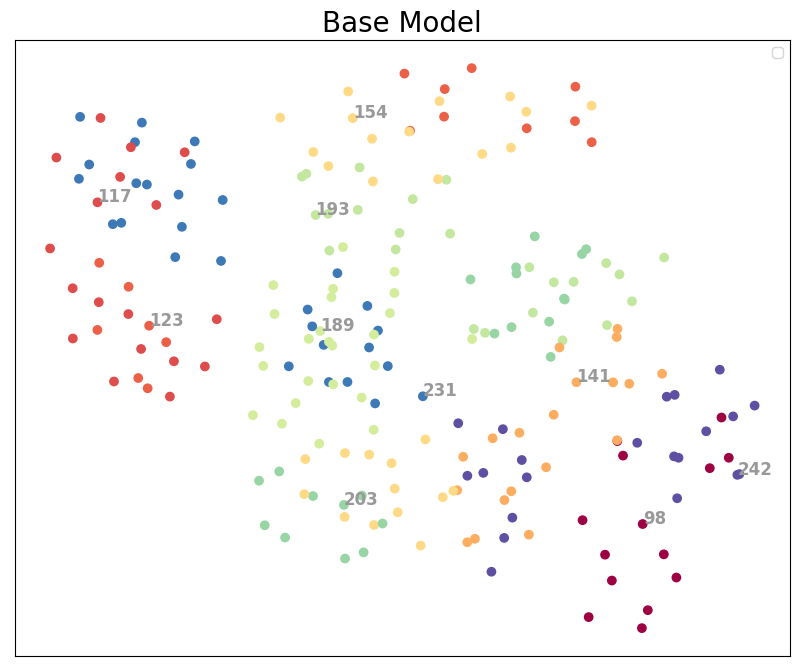
\includegraphics[width=0.42\linewidth]{t-SNE_68.55.png}}
  \subcaptionbox{\label{fig:tSNEb}}
    {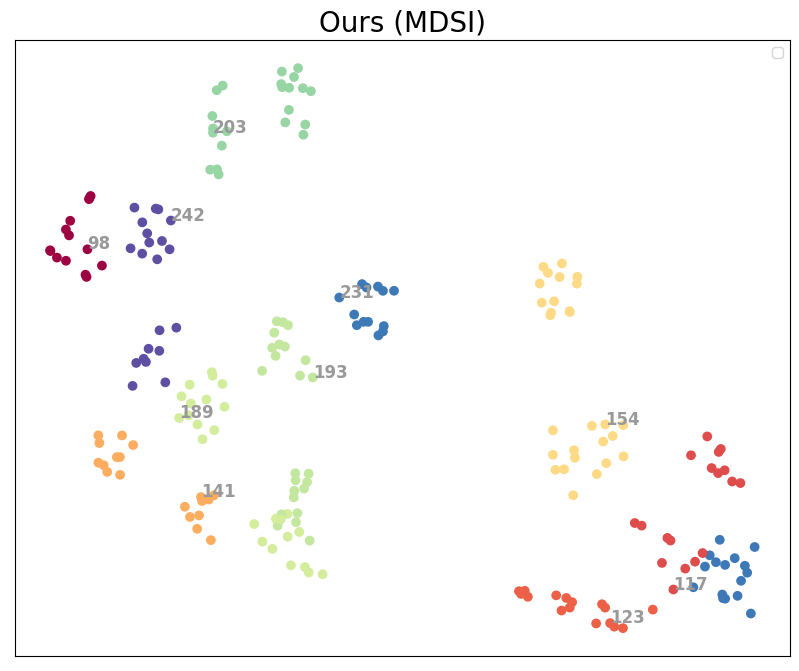
\includegraphics[width=0.42\linewidth]{t-SNE_75.07.png}}
  \subcaptionbox{\label{fig:confuse_base}}
    {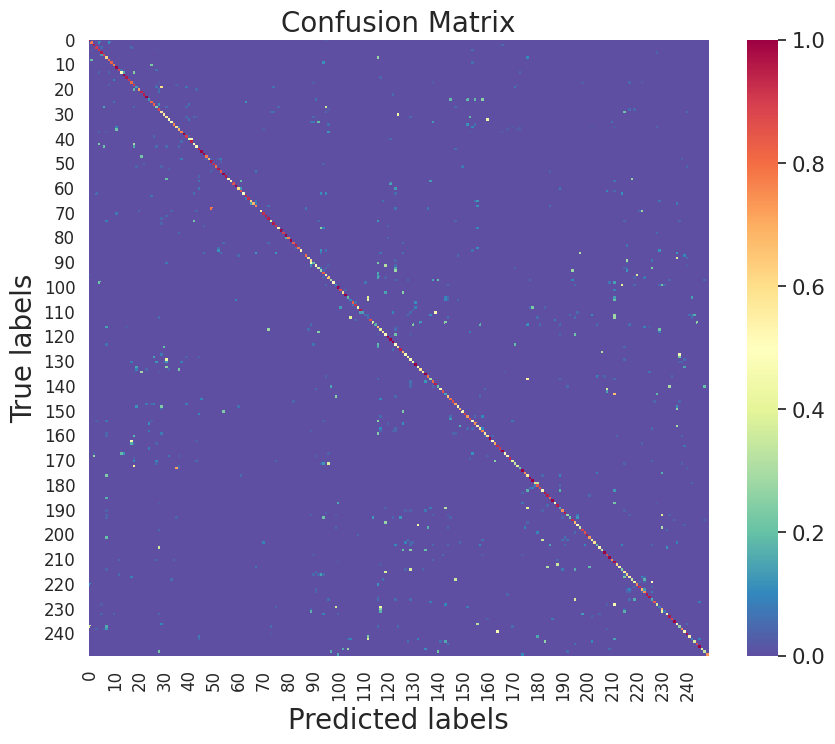
\includegraphics[width=0.49\linewidth]{confusion_matrix_59.85_spec.png}}
  \subcaptionbox{\label{fig:confuse_ours}}
    {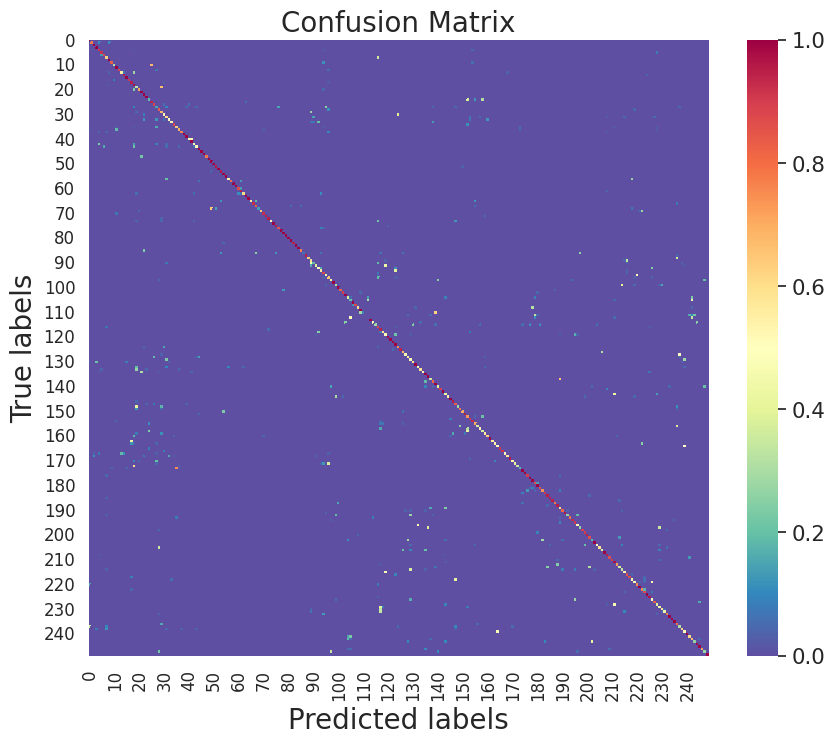
\includegraphics[width=0.49\linewidth]{confusion_matrix_75.07_spec.png}}
  \caption{可视化本文方法的增强效果。 (a) 基础模型的特征分布可视化。(b) MDSI 的特征分布可视化。(c) 基础模型的混淆矩阵。(d) MDSI 的混淆矩阵。}
  \label{fig:vis}
\end{figure}

\begin{figure}
  \centering
  \subcaptionbox{\label{fig:comp_gap}}
    {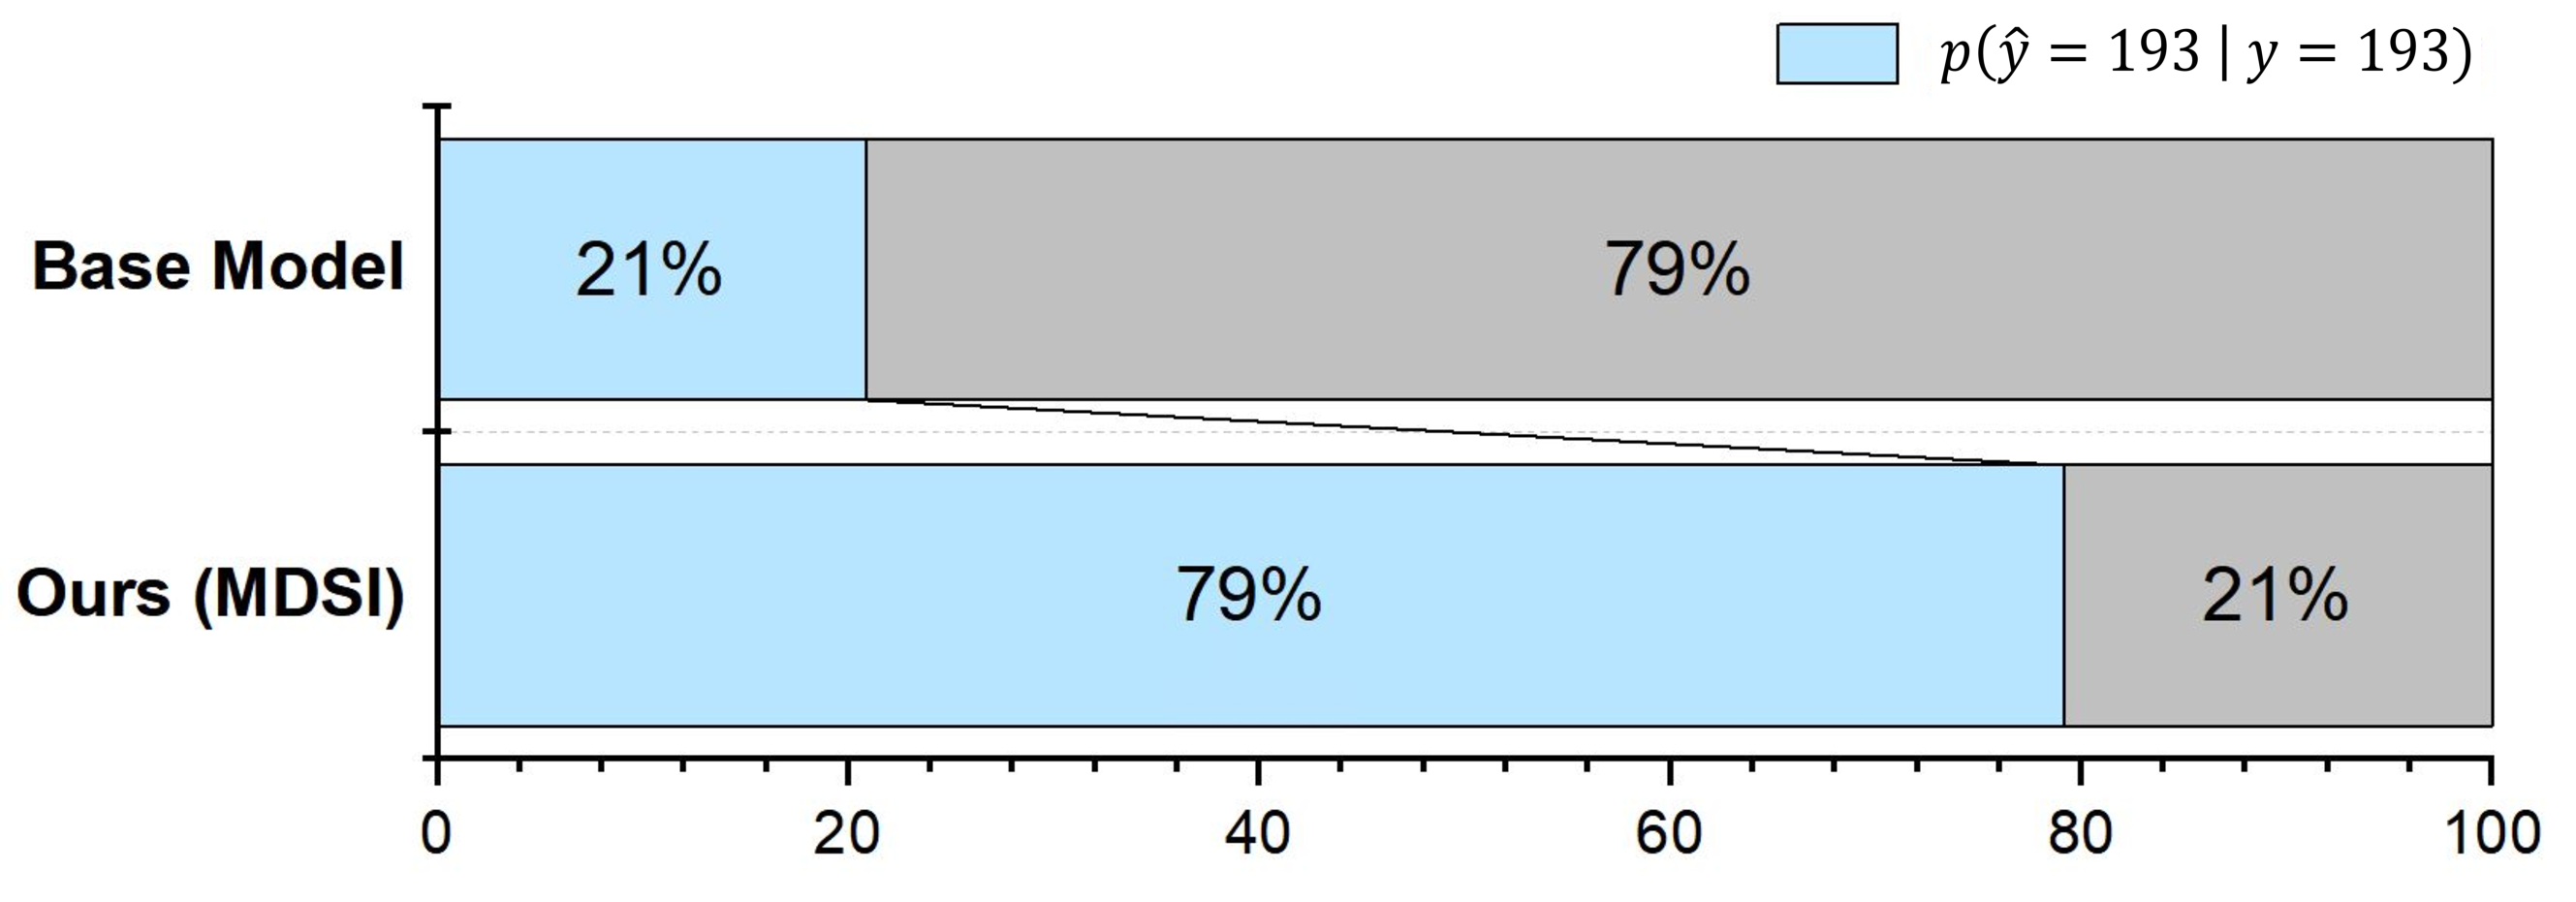
\includegraphics[width=0.49\linewidth]{comp_gap.pdf}}
  \subcaptionbox{\label{fig:comp_sim}}
    {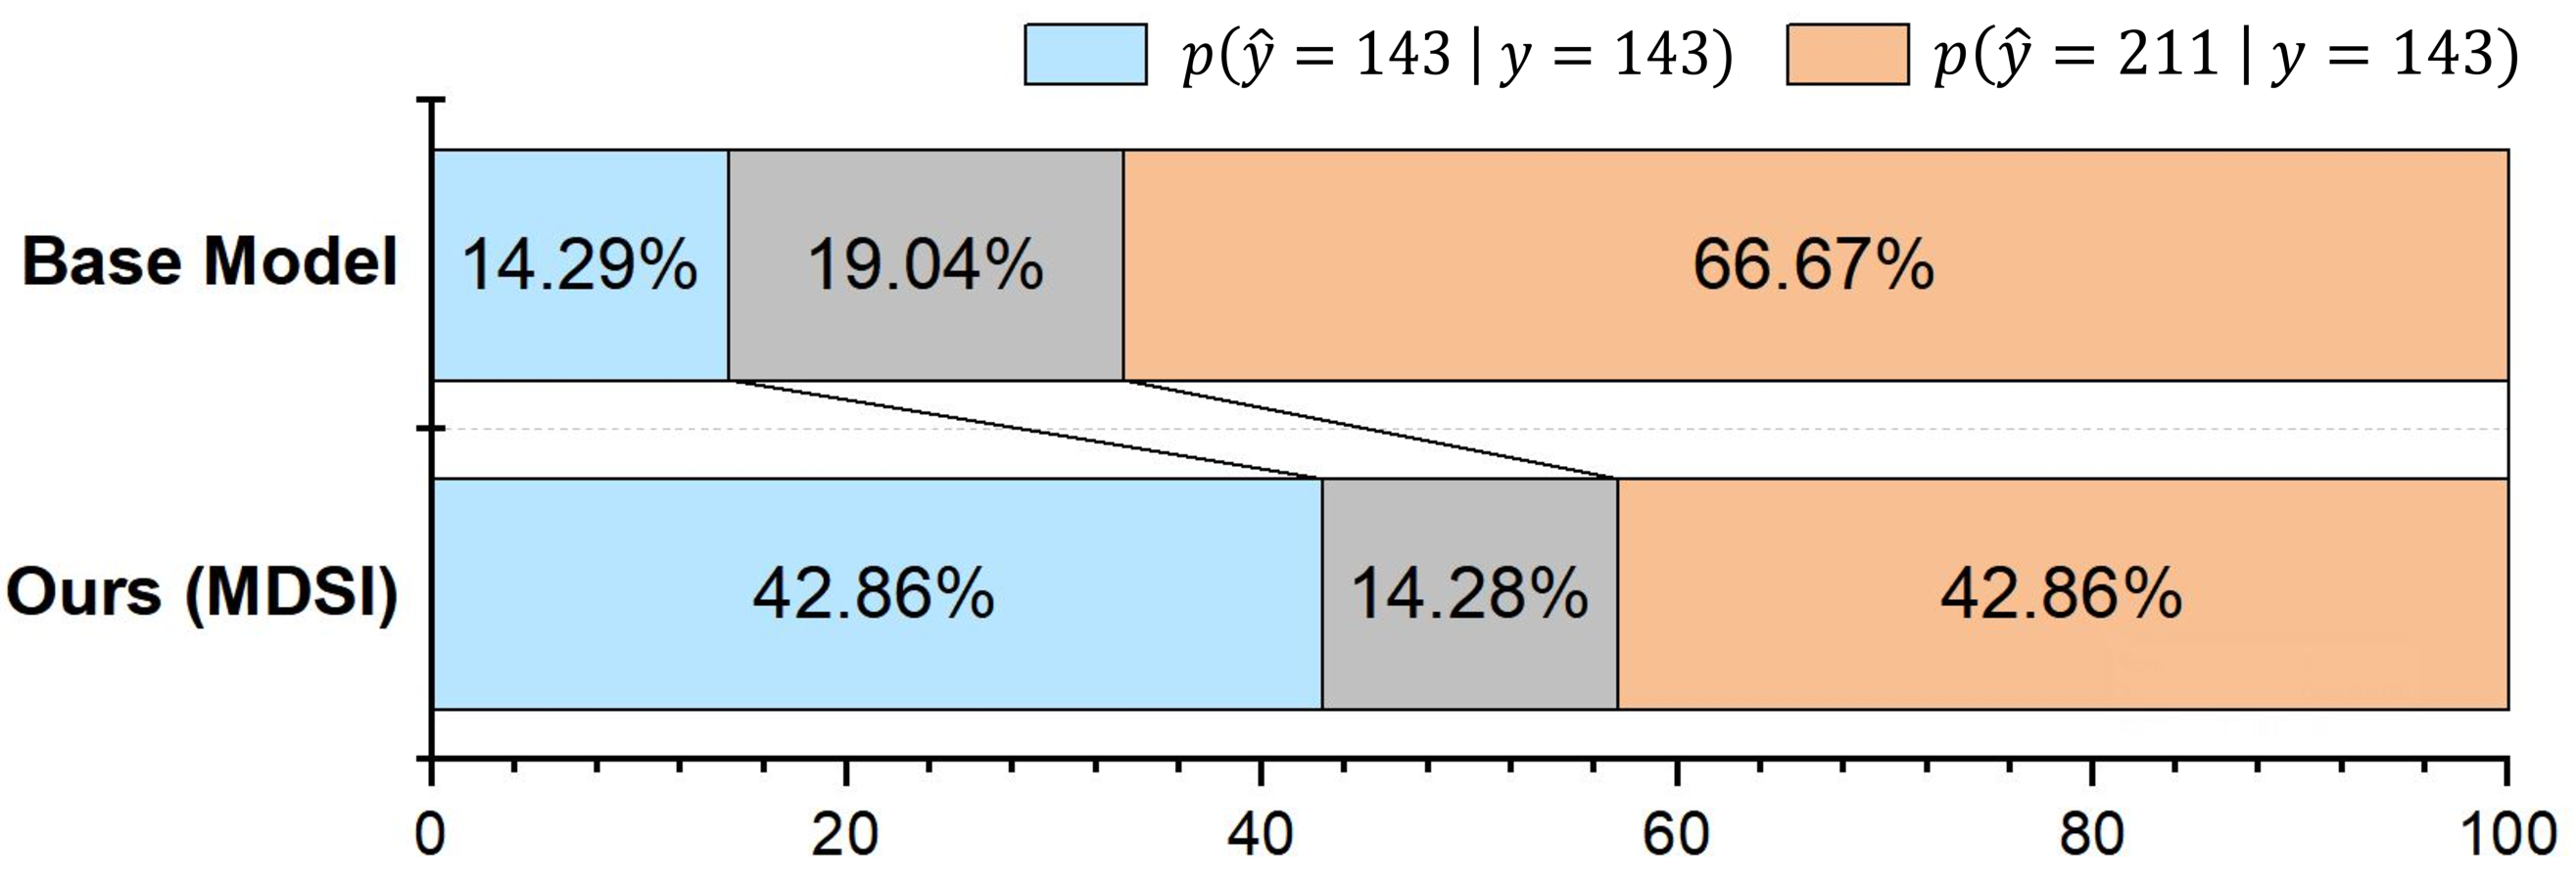
\includegraphics[width=0.49\linewidth]{comp_similar.pdf}}
  \caption{MDSI 在解决信息冗余 (IR) 和信息缺失 (IA) 挑战方面的增强效果。 (a) IR 场景下的性能改进(对应于图 ~\ref{fig:gap_sample} 中的样本)。 (b) IA 场景下的性能改进。(对应于图 ~\ref{fig:sim_sample} 中的样本)}
  \label{fig:comp}
\end{figure}

\subsubsection{定量和可视化结果}
为了进一步阐明本文方法的有效性,本文在图~\ref{fig:vis}中展示了 t-SNE 可视化和混淆矩阵。
此外,本文在图~\ref{fig:comp}中提供了统计结果,以突出 MDSI 在解决信息冗余 (IR) 和信息缺失 (IA) 挑战方面的改进。

在图~\ref{fig:tSNEa} 和 \ref{fig:tSNEb} 中,本文展示了基础模型和本文提出的 MDSI 方法的 t-SNE 可视化。
本文评估了与基础模型相比准确率提高最大的 10 个最具挑战性的类别。
基线模型 (图~\ref{fig:tSNEa}) 的视觉模式以相互交织的类别表示为特征,与本文的 MDSI (图~\ref{fig:tSNEb}) 实现的良好分离的聚类形成鲜明对比,这表明本文的 MDSI 有效地增强了特征表示的判别能力。
在图~\ref{fig:confuse_base} 和 \ref{fig:confuse_ours} 中,本文展示了基线模型和本文提出的 MDSI 的混淆矩阵。
矩阵显示,使用本文的方法,错误分类明显减少,说明了它通过最小化无关信息干扰来应对手势识别复杂性的卓越能力。
这种增强表明,所提出的方法不仅有效地增强了识别的鲁棒性和泛化能力,而且还增强了模型对关键手势特征的感知。

同时,本文对模型在信息冗余(IR)和信息缺失(IA)场景下的性能提升进行了详细分析。
考虑了图\ref{fig:samples}中描绘的两类样本对,图\ref{fig:comp_gap}和图~\ref{fig:comp_sim}分别说明了所提方法的影响。
MDSI带来的改进值得注意:i)对于遭受IR的样本类别,MDSI将准确率提高了58\%;ii)对于遭受IA的样本类别,MDSI将准确率提高了28.57\%,并将视觉相似类别的误分类率降低了23.81\%。
这些示例表明,本文的MDSI显着减轻了IR和IA对手势识别的影响,确保了稳健和通用的性能。


\section{本章小结}
针对手部动作评估问题,本章提出了一种可插拔的多模态动态手势识别算法,称为多策略解耦与语义集成(MDSI),旨在解决RGB-D手势识别中的信息冗余(IR)和信息缺失(IA)挑战。
首先,第~\ref{sec:MDN}节引入了多策略解耦网络(MDN),通过解耦“姿态-运动”和“时空-通道”特征来减轻冗余信息。
随后,第~\ref{sec:SIN}节提出了语义集成网络(SIN),该网络通过语义过滤和标签平滑增强语义理解,有效地指导视觉相似手势的区分。
MDSI的可插拔特性使其能够以最小的计算开销无缝集成到各种视频编码器架构中,展示了其在动作识别和手语识别等相关领域的扩展潜力。大量实验(第~\ref{sec:GR_EXP}节)表明,MDSI在两个广泛认可的基准测试中超越了先前的最先进方法,展现了其在手语教学动作评估中的实际应用潜力。
% 本文预计通过进一步改进MDSI和优化预处理将增强其实时部署能力。


% 理论依据:部分属于SOTA方法的有机结合

% \subsection{现阶段实验结果与讨论}
% \subsubsection{实验设置}
% 现阶段实验主要围绕GRGB分支(图\ref{fig:多流解耦注意力手势识别网络})展开,本文基于所提出的循环手势识别变换器(RGRT,图\ref{fig:RGRT})搭建了GRGB分支,并进行了一系列实验以验证RGRT在手势时空建模方面的有效性。
% 本文在大规模孤立手势数据集Jester-V1~\cite{jester2017}上进行预训练,并基于 ChaLearn LAP 孤立手势数据集IsoGD\cite{wan2016chalearn} 评估本文的动态手势识别算法。
% \paragraph{Jester数据集}~\cite{jester2017}。Jester是大量带有密集标签的视频剪辑的集合,是目前最大的孤立手势数据集。每个剪辑都包含工作人员在笔记本电脑摄像头或网络摄像头前执行的预定义手势。该数据集包含 27 种手势的 148094 个 RGB 视频文件,其中每个类别平均有超过 5000 个实例。
% \paragraph{IsoGD数据集}\cite{wan2016chalearn}。ChaLearn LAP RGB-D 孤立手势数据集(IsoGD)是一个用于手势识别的大型多模态数据集。该数据集包含 21 个不同个体执行的 249 个手势标签,共计47933个RGB-D手势视频实例。IsoGD由Microsoft Kinect传感器记录,包括传感器提供的RGB和Depth视频序列。
% \begin{figure}
%   \centering
%   \subcaptionbox{手势ID:50\label{fig:sa}}
%     {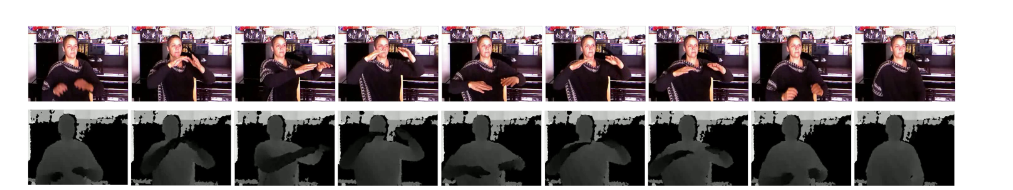
\includegraphics[width=0.75\linewidth]{samplesa.png}}
%   \subcaptionbox{手势ID:138\label{fig:sb}}
%     {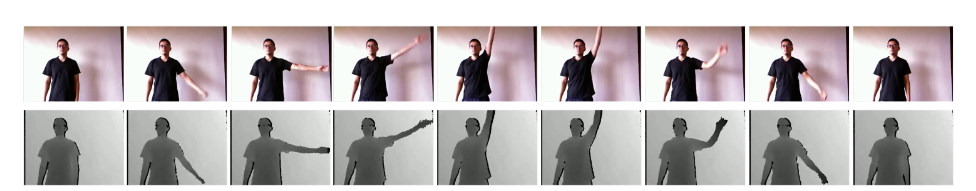
\includegraphics[width=0.75\linewidth]{samplesb.png}}
%   \caption{IsoGD\cite{wan2016chalearn}数据集动态手势样本示例}
%   \label{fig:samples}
% \end{figure}

% % AUTSL手语数据集。
% \subsubsection{RGRT效果分析} % 报告Jester和IsoGD
% 本文分别构建了基于所提出的循环手势识别变换器(RGRT)和基于不含变换器的循环模型的GRGB分支,并进行了对比实验。如表\ref{tab:ablation}结果所示,RGRT能够有效提升动态手势识别的准确率。这是由于RGRT网络巧妙地将循环结构与局部时域变换器(TWT)有效地结合,实现了多尺度时空建模。
% \begin{table}
%   \centering
%   \caption{GRGB分支消融分析}
%   \begin{tabular}{ccc}
%     \toprule
%     \multirow{2}{*}{Model} & \multicolumn{2}{c}{Accuracy(\%)}\\
%  & Jester\_val  & IsoGD\_val \\
%     \midrule
%     -w/o RGRT   & 93.60 & 55.71\\
%     Ours    & 94.07 & 56.67 \\
%     \bottomrule
%   \end{tabular}
%   \label{tab:ablation}
% \end{table}


% \subsubsection{与SOTA方法的比较} % 目前对比不使用额外通道的方法 % 报告IsoGD上的对比
% 本文将包含RGRT的GRGB分支网络与最先进的端到端手势识别网络进行了比较(如表\ref{tab:comparison}所示)。在IsoGD验证集上,本文的方法在RGB模态上取得了第二名的具有竞争力的识别性能,实现了56.67\%的准确率。仅略低于Zhu等人的方法\cite{zhu2019redundancy}(-0.75\%)。这可能是由于Zhu等人在汇报最终结果时使用了金字塔策略\cite{zhu2016large},对同一手势视频划分多段并融合预测。在后续工作中,本文计划对齐相关输入预处理技术,以更全面地比较模型性能。
% 上述实验结果突显了本文提出的包含RGRT的GRGB分支网络在手势时空建模方面的有效性,为后续解耦手势识别的研究打下了基础。
% \begin{table}
%   \centering
%   \caption{GRGB分支在IsoGD验证集上与SOTA方法的比较}
%   \begin{tabular}{lc}
%     \toprule
%     Method & Accuracy(\%)\\
%     \midrule
%     ResNet50\cite{narayana2018focus} & 33.22 \\
%     Pyramidal C3D\cite{zhu2016large}  & 36.58 \\
%     32-frame C3D\cite{li2016large} & 37.30 \\
%     8-MFFs-0f1c\cite{kopuklu2018motion} & 41.30 \\
%     Res3D\cite{miao2017multimodal} & 45.07 \\
%     3DCNN+BiConvLSTM+2DCNN\cite{zhang2017learning} &  51.31 \\
%     Res3D+ConvLSTM+MobileNet\cite{zhu2018continuous}  & 52.01 \\
%     ConvLSTMForGR\cite{zhu2019redundancy} & 55.98 \\
%     ConvLSTMForGR+Pyramid\cite{zhu2019redundancy} & 57.42 \\
%     \midrule
%     Ours -w/o RGRT & 55.71 \\
%     Ours & 56.67    \\
%     \bottomrule
%   \end{tabular}
%   \label{tab:comparison}
% \end{table}

% \subsubsection{推理速度}
% 本文在单张RTX2080显卡上对GRGB分支模型进行了推理速度测试,对同一样本进行了五次测试。如图\ref{fig:time}所示,GRGB分支的平均推理时间为83.9ms,快于范等人\cite{范桂双2020基于S3D}所公布的96ms。这表明本文的网络具有高效的推理能力。本文计划在后续工作中进一步优化网络结构,以进一步提升模型的推理速度。

% \begin{figure}
%   \centering
%   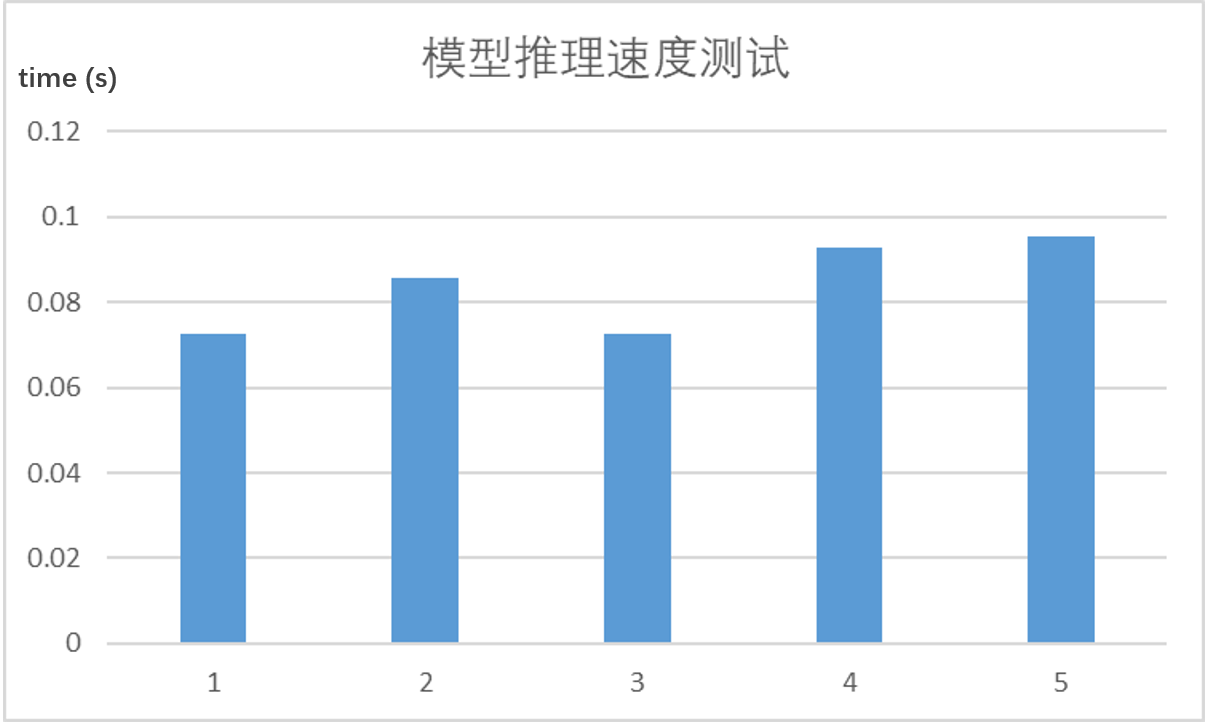
\includegraphics[width=0.65\linewidth]{time.png}
%   % \caption*{}
%   \caption{GRGB分支模型推理时间(单位:s)}
%   \label{fig:time}
% \end{figure}

% \subsubsection{解耦手势数据处理}
% 本文使用HRNet\cite{sun2019deep}在上述数据集上事先提取并保存二维骨架数据(如图\ref{fig:8b}),随后进行手势解耦。目前,本文已经完成了Jester数据集上的解耦手势数据处理,后续将基于此开展解耦识别网络实验。
  % 多模态手势识别算法研究
% !TeX root = ../thuthesis-example.tex

% \chapter{研究方法}
\chapter{基于手势描述的协同手势生成算法研究}
\label{sec:GG} 
为了缓解手语教学中标准示范资源缺乏的问题,本章提出了一种描述驱动的协同手势生成框架(如图\ref{fig:teaser}所示)。
首先,本文引入了一种统一的运动表示方法,将不同来源的运动数据嵌入到紧凑的潜在空间中(第\ref{sec:method:m_rep}节)。在此基础上,本文设计了一种可控的手势潜在扩散模型(第\ref{sec:method:gld}节),该模型包含两个关键组件:
(1) 一个手势变分自编码器,用于学习手势的低维潜在表示;
(2) 一个在该潜在空间中高效运行的分层条件扩散模型。
为了实现语义和节奏的协同精确控制,本文提出了一种手势描述框架(第\ref{sec:method:caption}节),该框架利用运动-语言模型为手势数据生成描述性文本标注,填补了手势数据描述性文本标注的空白。
此外,本文还设计了一种多粒度描述控制机制(第\ref{sec:method:control}节)以确保精确的语义注入。
大量实验表明,所提出的方法能够有效生成高质量、语义一致、节奏同步的手势,为手语示范动作的扩充生成提供了有力支持。

\begin{figure*}[!h]
  \centering
  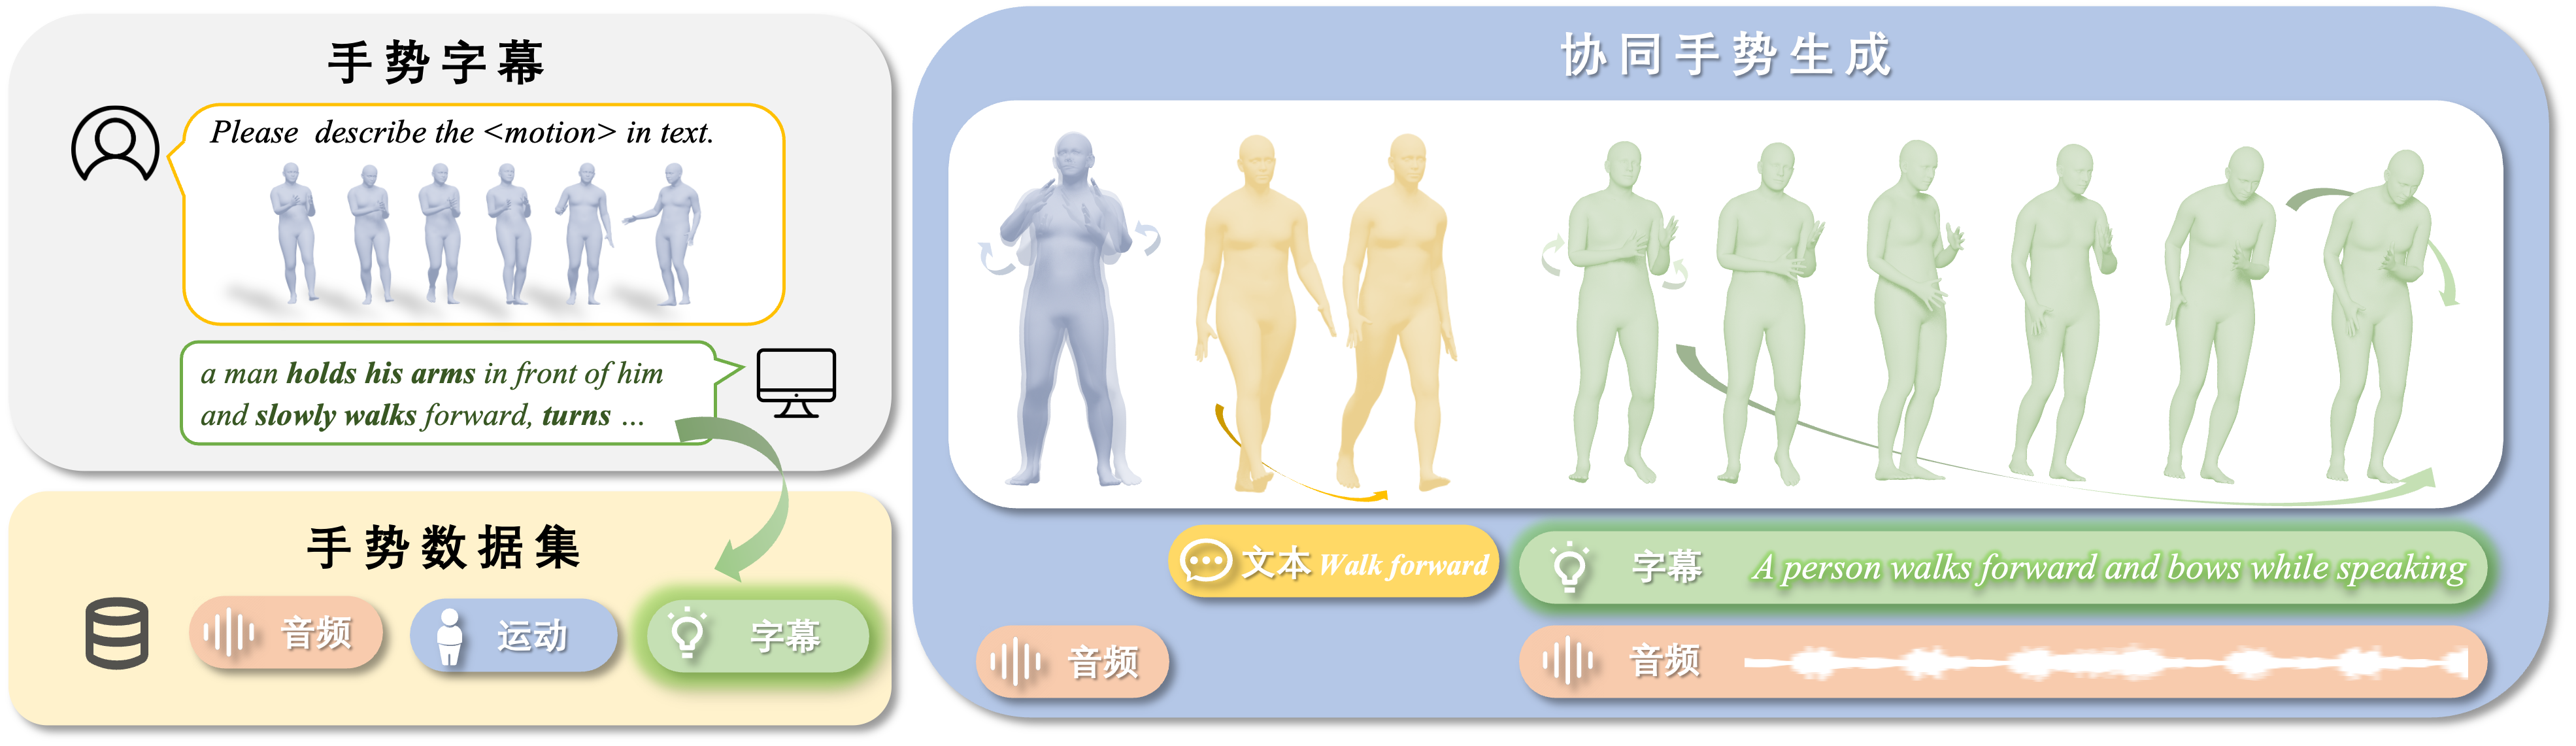
\includegraphics[width=\linewidth]{teaser.png}
  \caption{\textbf{CoordSpeaker} 支持手势字幕和定制的协同的说话者动作生成,既能与字幕保持语义一致,又能与音频保持节奏同步。例如,在演讲场景中,本文的方法允许说话者在讲话时自然地向前走并鞠躬,无缝地做出结束手势。} %Our method generates natural speaking gestures synchronized with speech and text captions. Given speech and text prompts (such as ``sitting'', ``waving while talking'', etc.), our model produces coordinated gesture motions that align with both speech rhythm and textual semantics. The figure above demonstrates gesture examples generated under the same speech with different text prompts.}
  \label{fig:teaser}
\end{figure*}

\section{运动表示}
\label{sec:method:m_rep}
为了将不同来源的运动数据统一到紧凑的潜在空间中,本文实现了一种紧凑的运动表示方法。首先将各种数据格式转换为统一的HumanML3D格式表示,然后通过本文的运动编码器$\mathcal{E}$(在第\ref{sec:method:gld}节中描述)将其映射到一个具有代表性的潜在空间。
% [freetalker: ...->humanml3d]
% We expect that the features of the different motion datasets are correctly preserved. In contrast to [16] and [17], where [16] represents human motions with discrete codes and [17] retargets human motion to a homograph consisting of five terminal joints (head, hands, and feet), potentially losing important detailed information such as shoulders and fingers, our approach addresses this issue and preserves motion details. We first convert the rotation matrix of the motion capture (BVH format) data to an axis angle representation of SMPL-X [20]. For the 3D position dataset, we fit it to the SMPL-X representation using VPoser [20]. We then scale the 3D translations of the root joint appropriately and adjust the initial orientation to be uniform across the different datasets as [17]. With the SMPL-X model forward computation, we can obtain the 3D position of the SMPL-X representation. Then as in [21], we use root height, root linear and rotational velocity, joint rotation, joint position, joint velocity, and foot contact as kinematic feature representations. Each frame of the processed motion sequence has 659 dimensional features, which we denote as xˆ0 ∈ RTM ×659, where TM denotes the number of motion sequence frames.

\subsection{统一运动表示}
\label{sec:method:m_rep:unified}
% 22joints->nfeats=263(用于输入motionllm生成description), 55joints->nfeats=659(用于输入gld训练)
% [mld] HumanML3D Format [17] proposes a motion representation x1:L inspired by motion features in character control [66, 45, 65]. This redundant representation is quite suited to neural models, particularly variational autoencoders. Specifically, the i-th pose xi is defined by a tuple of root angular velocity r ̇a ∈ R along Y-axis, root linear velocities (r ̇x, r ̇z ∈ R) on XZ-plane, root height ry ∈ R, local joints positions jp ∈ R3Nj , velocities jv ∈ R3Nj and rotations jr ∈ R6Nj in root space, and binary foot-ground contact features cf ∈ R4 by thresholding the heel and toe joint velocities, where Nj denotes the joint number, giving:  xi = {r ̇a, r ̇x, r ̇z, ry, jp, jv, jr, cf }.
为了利用额外人体运动数据集中的语义先验知识,本文采用HumanML3D~\cite{guo2022humanml3d}并将不同的运动数据统一到一个一致的特征空间中。
参照~\cite{yang2024freetalker,guo2022humanml3d},第$i$帧运动被表示为$x^i=\left\{\dot{r}^a, \dot{r}^x, \dot{r}^z, r^y, \mathbf{j}^p, \mathbf{j}^v, \mathbf{j}^r, \mathbf{c}^f\right\}$,其中$\dot{r}^a, \dot{r}^x, \dot{r}^z, r^y$表示根关节的角速度、线速度和高度,$\mathbf{j}^p, \mathbf{j}^v, \mathbf{j}^r$表示关节位置、速度和旋转,$\mathbf{c}^f$表示足部接触特征。
虽然原始HumanML3D格式遵循SMPL~\cite{loper2023smpl}骨架的22个关节,但本文将其扩展到55个关节以更好地适应手势数据。因此,每一帧运动被表示为659维特征向量,记为$x \in \mathbb{R}^{T\times 659}$,其中$T$为序列长度。


\subsection{潜在表示}
近期研究表明,潜在表示在神经运动建模中发挥着关键作用。
本文采用基于Transformer的VAE模型将运动序列编码到紧凑且信息丰富的潜在空间中,该模型由编码器$\mathcal{E}$和解码器$\mathcal{D}$组成,并通过长跳跃连接来保持运动细节。
具体而言,运动序列$x^{1:L}$首先通过编码器$\mathcal{E}$编码为潜在向量$z \in \mathbb{R}^{n\times d}$,其中$d$表示潜在维度。编码器接收逐帧运动特征和可学习的分布令牌作为输入,生成运动潜在空间的高斯分布参数$\mu$和$\sigma$。这些参数通过标准VAE采样过程重参数化得到潜在向量。
对于运动解码,$\mathcal{D}$采用带有交叉注意力机制的Transformer架构。它以零运动令牌作为查询,潜在向量$z$作为键和值,生成重建的运动序列$\hat{x}^{1:L}$。整个VAE通过均方误差(MSE)和Kullback-Leibler(KL)散度的组合进行训练:
\begin{equation}
L_{\text{VAE}} = \|x^{1:L} - \hat{x}^{1:L}\|_2^2 + \beta \text{KL}(q_{\phi}(z|x^{1:L})\|p(z))
\label{eq:loss_vae}
\end{equation}
其中$\beta$平衡重建和正则化项。这种潜在表示方法在保持运动保真度和多样性的同时实现了高效的手势合成。
% [mld] Latent Format [40]. Latent representations are widely used in neural models [46, 47, 19, 9]. We recognize it as motion representation in latent space. By leveraging VAE models, latent vectors can represent plausible motions as:  xˆ1:L = D(z), z = E(x1:L)
% [mld: ...->latents]
% We build our motion Variational AutoEncoder, V, based on a transformer-based architecture [46], which consists of a transformer encoder E and a transformer decoder D. The motion VAE, V = {E, D}, is trained by the motion x1:L reconstruction only with the Mean Squared Error (MSE) loss and the Kullback-Leibler (KL) loss. We further enhance two transformers [70] of E and D with long skip connections [59], and remove the action biases used in [46]. The encoder could produce a representative, low-dimensional latent space with high informative density, and the decoder could well reconstruct the latent into motion sequences. More specifically, the motion encoder E takes as input learnable distribution tokens, and frame-wise motion features x1:L of arbitrary length L. We use the embedded distribution tokens as Gaussian distribution parameters μ and σ of the motion latent space Z to reparameterize [30] latent z ∈ Rn×d whose dimension is similar to [46]. The motion decoder D relies on the architecture of the transformer decoder with cross attention mechanism, which takes the L number of zero motion tokes as queries, a latent z ∈ Rn×d as memory, and finally, generates a human motion sequence xˆ1:L with L frames. According to [47], both the latent space Z and variable durations help the model to produce more diverse motions. To further enhance the latent representation, we leverage a long skip-connection structure for the transformer-based encoder E and decoder D. We also explore the effectiveness of the latent’s dimensions on motion sequences representation in Tab. 4. Hence, our VAE models present a stronger motion reconstruction ability and richer diversity (cf. Tab. 5 and Tab. 6). We provide more details about the architecture and the training in the supplementary.

% [syntalker] 3.2 Motion Representation Module  Motion encoding. Recent studies in motion generation have demonstrated that vector-quantized autoencoder (VQ-VAE) [44] possesses a remarkable capability for compressing motion information [2, 17, 55]. We also utilize vector quantization for motion encoding. Following [17, 33, 54], we use a residual VQ-VAE (RVQ-VAE) as the quantization layer. To further decrease the coupling between body parts, we segment the body into three parts: upper body, fingers, and lower body, like in [2, 28], and train a separate RVQ-VAE for each part. In details, the motion sequence M can be represented as m1:N ∈ RN ×D , which is firstly encoded into a latent vector sequence z1:n ∈ Rn×d with downsampling ratio of n/N and latent dimension d, using 1D convolutional encoder E; The z1:n ∈ Rn×d obtained through the encoder then enters the first quantization layer Q1, each vector subsequently finds its nearest code entry in the layer’s codebook C1 = {c1  k }K  k=1 ⊂ Rd to get the  first quantization code ˆz1  1:n, also we can calculate the quantization  residual1:n = ˆz1  1:n − z1:n. The residual1:n then enter the second quantization layer Q2 finds its nearest code entry in the layer’s codebook C2 = {c2  k }K  k=1 ⊂ Rd to get the second quantization code  ˆz21:n. Accordingly, ˆz3  1:n,ˆz4  1:n... can be calculated in this manner. As the last step of motion encoding, we sum all quantization code together to get the final code zˆ = ÍQ  q=1 ˆzv .  Motion decoding. Similar to motion encoding, three separated decoders are introduced for generating corresponding motions for all body parts, which are 1D convolutional decoders. During training, the motion data is encoded with motion encoders and fused with speech and prompt conditions by the diffusion-based conditional generation module, and then passed through the decoders to get the reconstructed motions. During inference, the motion encoder is not utilized, the generated motion is obtained directly from the speech and prompt conditions with the diffusion module and motion decoders.

\begin{figure*}[t]
  \centering
  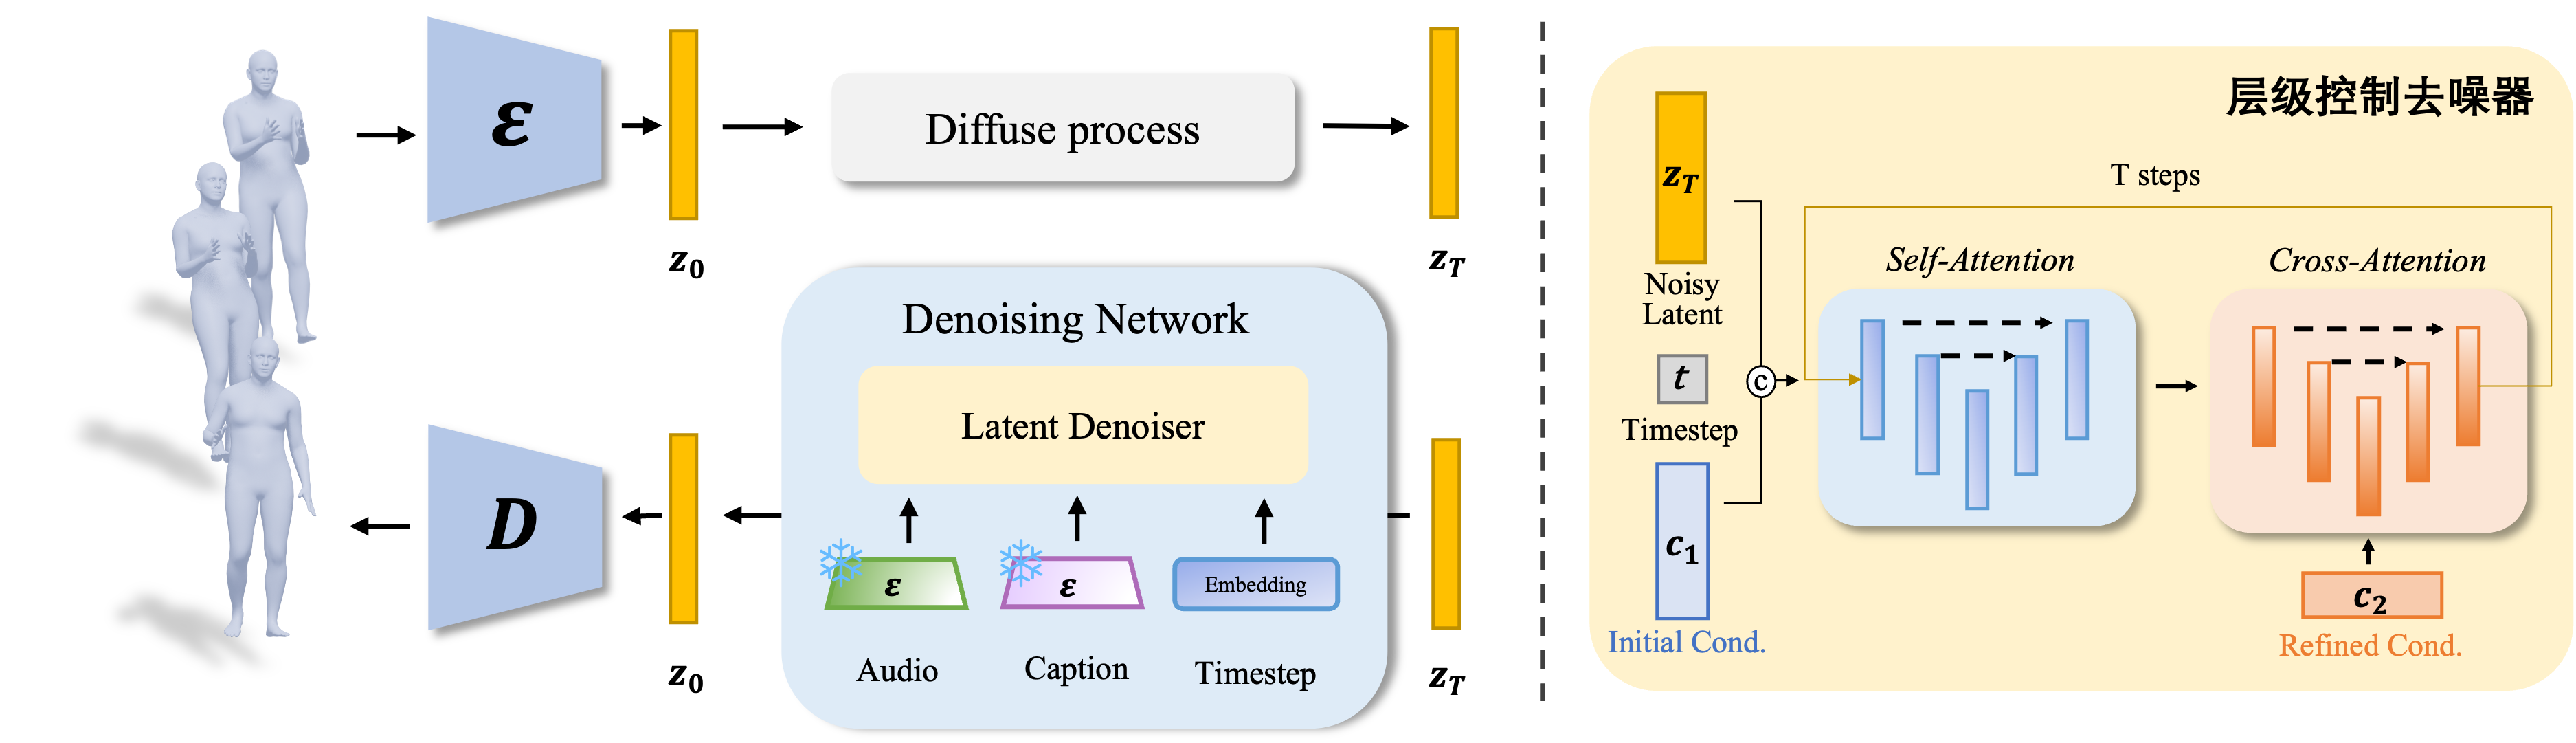
\includegraphics[width=\linewidth]{model_v1_zh.png}
  \caption{协同手势生成模型概览。本文的条件潜在扩散模型(第~\ref{sec:method:gld}节)由两个关键组件组成:(1)手势变分自动编码器,可学习统一的低维潜在表示,从而实现紧凑的跨数据集运动建模,以及(2)分层控制的降噪器,确保分层条件注入并在该学习到的潜在空间中有效运行。}
  \label{fig:method:model}
\end{figure*}
\section{可控手势潜在扩散模型}
\label{sec:method:gld}
% Diffusion model 出于其强大的生成质量与多样性,已经在图像、音频、视频、运动生成等领域取得了显著成果 \cite{}。一些工作在原始运动空间针对运动序列进行diffusion,但存在效率低下与高频噪声的问题\cite{}。本文基于latent space进行diffusion,旨在生成隐变量z∈ Rn×d,可以显著提高效率。
基于VAE学习的紧凑潜在表示,本文提出了一种可控手势潜在扩散模型,用于生成高质量手势。与以前直接在原始运动序列上执行扩散的方法不同,本文的模型通过对潜在向量进行操作,显著降低了计算要求,同时保持了生成质量。
% mld(optional改进)
% 3.2. Motion Latent Diffusion Model  Diffusion probabilistic models [63] can gradually anneal the noise from a gaussian distribution to a data distribution p(x) by learning the noise prediction from a T length Markov noising process, giving {xt}tT=1. It leads to a significant influence in many research domains, such as the most famous image synthesis models [11, 23, 62, 56], the density estimation model [29] and the motion generation models [69, 75]. For motion generation, these works train the diffusion models with a transformer-based denoiser θ (xt, t), which anneal the random noise to motion sequence {xˆ1:N  t }tT=1 iteratively. However, diffusion on raw motion sequences is inefficient and requires exhausting computational resources. Besides, raw motion data from the markless or marker-based motion capture system usually remain high-frequency outliers, which might have a side effect on the diffusion model to learn the actual data distribution. To reduce the computational requirements of the diffusion models on raw motion sequences and improve the synthesized quality, we perform the diffusion process on a representative and lowdimensional motion latent space. Here, we introduce our denoiser θ. Different from the previous UNet-based architecture [59] on the 2D image latent zI , we build a transformer-based denoising model with long skip connections [4] on the motion latent z ∈ Rn×d, which is more suitable for sequential data, like human motion sequences. The diffusion on latent space is modeled as a Markov nosing process using:  q (zt | zt−1) = N (√αtzt−1, (1 − αt) I) .   where the constant αt ∈ (0, 1) is a hyper-parameters for sampling. We then use {zt}tT=0 to denote the noising sequence, and zt−1 = θ (zt, t) for the t-step denoising. We further focus on the unconditional generation with the simple objective [23]:  LMLD := E ,t  [  ‖ − θ (zt, t)‖2  2  ]  , where ∼ N (0, 1), z0 = E(x1:L). During the training of θ, the encoder E is frozen to compress motion into z0. The samples of the diffusion forward process are from the latent distribution p(z0). During the diffusion reverse stage, θ first predict zˆ0 with T iterative denoising steps, then D decodes zˆ0 to motion results with one forward.

\subsection{潜在扩散过程}
潜在空间中的扩散过程遵循马尔可夫链,逐步向潜在向量$\mathbf{z} \in \mathbb{R}^{n\times d}$添加高斯噪声。对于噪声步骤$t \in [1,T]$,前向过程定义为:
\begin{equation}
  q(z_t|z_{t-1}) = \mathcal{N}(\sqrt{\alpha_t}z_{t-1}, (1-\alpha_t)\mathbf{I}),
\end{equation}
其中$\alpha_t \in (0,1)$是常数方差调度,且$z_T \sim \mathcal{N}(0, \mathbf{I})$。
为了生成高质量手势,本文采用基于Transformer的去噪器$\epsilon_\theta$来迭代预测和去除噪声。从随机噪声$z_T$开始,去噪器逐步恢复潜在向量$\hat{z}_0$,然后通过$\mathcal{D}$解码为手势运动。去噪过程同时受音频特征$\mathbf{A}$和描述嵌入$\mathbf{C}$的条件约束。

\subsection{分层条件注入}
为了实现对手势生成的精确多模态控制,本文的模型通过精心设计的嵌入和分层注入过程整合多个条件。
% 本文采用CLIP文本编码器~\cite{radford2021clip}和WavLM编码器~\cite{chen2022wavlm}分别从描述和音频中提取语义特征$\mathbf{C} \in \mathbb{R}^{512}$和声学特征$\mathbf{A} \in \mathbb{R}^{T\times1133}$。提取的特征通过特定模态的嵌入层进一步处理以获得最终的条件嵌入。
对于字幕编码,使用预训练的CLIP文本编码器~\cite{radford2021clip} 提取语义特征 $\mathbf{C} \in \mathbb{R}^{512}$。使用WavLM编码器~\cite{chen2022wavlm} 提取音频特征 $\mathbf{A} \in \mathbb{R}^{T\times1133}$,捕获丰富的声学信息,包括韵律和节奏模式。然后通过特定于模态的嵌入层处理这些原始特征,以形成条件嵌入 $\mathbf{C}$ 和 $\mathbf{A}$。
此外,为了实现更灵活和精确的生成控制,本文提出了一种分层条件注入机制,包含两个阶段(图\ref{fig:method:model}):
首先,初始条件$\mathbf{c_1}$与噪声潜在向量和时间步嵌入串联后输入去噪器$\epsilon_\theta$,提供基本指导。
其次,细化条件$\mathbf{c_2}$通过交叉注意力机制在去噪器内部整合,实现精细的控制调整。

\subsection{无分类器指导}
为了增强生成手势的质量和可控性,本文在训练和推理过程中采用无分类器指导\cite{ho2022classifier}。在训练过程中,随机屏蔽10\%的条件输入以同时学习有条件和无条件分布。在推理过程中,噪声预测通过不同指导的预测加权组合计算:
\begin{equation}
  \begin{split}
      \epsilon_\theta^s(z_t, t, \mathbf{c}) = & s_1 \epsilon_\theta(z_t, t, \mathbf{c}=\{\varnothing, \mathbf{A}\}) \\
      & + s_2 \epsilon_\theta(z_t, t, \mathbf{c}=\{\mathbf{C}, \varnothing\}) \\
      & + (1 - s_1 - s_2) \epsilon_\theta(z_t, t, \mathbf{c}=\{\varnothing, \varnothing\}),
  \end{split}
\end{equation}
其中$s_1$、$s_2$分别是音频和描述的指导尺度,且$s_1, s_2 > 1$可以增强其效果。
这种方法允许对描述和音频分别应用指导,在手势生成过程中实现更精确的条件控制。

\subsection{训练与推理}
潜在扩散模型使用简单的$\ell_2$目标进行训练\cite{ho2020ddpm, chen2023executing}:
\begin{equation}
  \mathcal{L}_{\text{Diff}} = \mathbb{E}_{\epsilon,t}[\|\epsilon - \epsilon_\theta(z_t, t, c)\|_2^2],
\end{equation}
其中$\epsilon \sim \mathcal{N}(0,\mathbf{I})$且$z_0 = \mathcal{E}(x^{1:L})$。在推理过程中,本文的模型首先通过$T$个去噪步骤预测潜在向量$\hat{z}_0$,然后通过解码器$\mathcal{D}$的单次前向传播将其解码为运动序列$\hat{x}^{1:L}$。

\begin{figure*}[t]
  \centering
  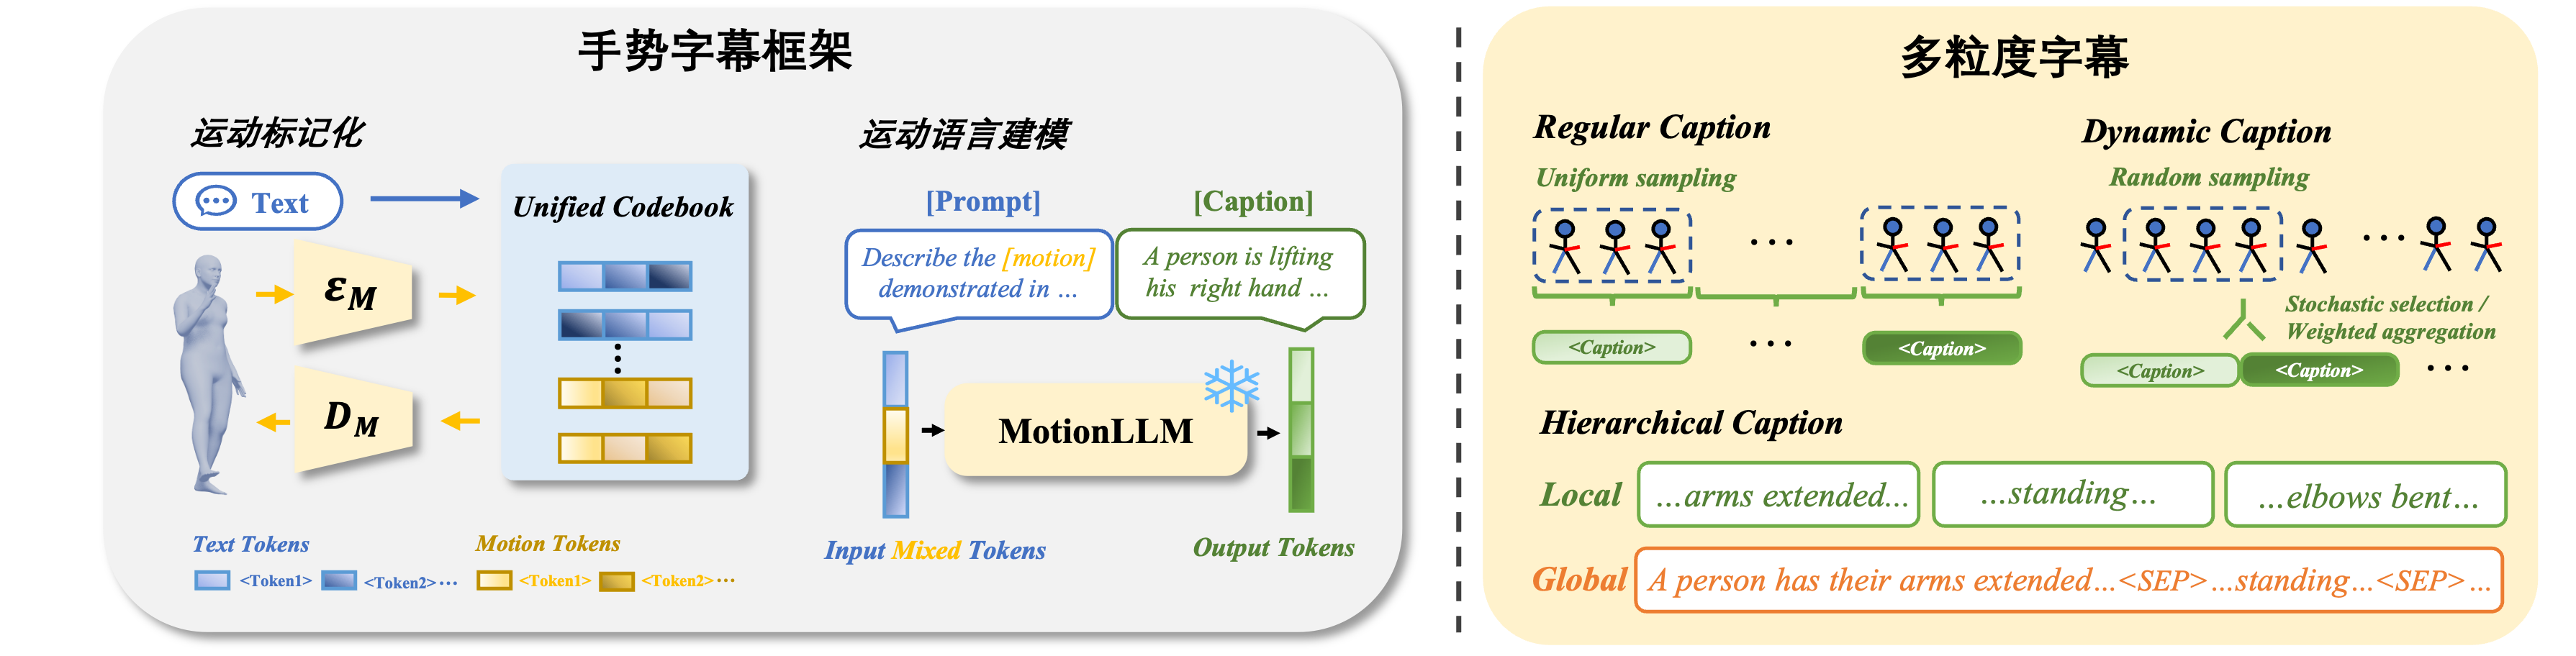
\includegraphics[width=\linewidth]{gesture_captioning_v1_zh.png}
  \caption{手势描述生成框架。本文的手势描述生成框架包含两个主要组件:
  运动分词器和运动感知语言模型。运动分词器将手势序列编码为离散的运动token序列,运动感知语
  言模型则基于这些token和提示模板生成对应的手势描述。}
  \label{fig:method:captioning}
\end{figure*}

\section{手势描述}
\label{sec:method:caption}
手势数据缺乏描述性文本标注显著限制了通过文本提示控制手势合成的能力~\cite{chen2024syntalker}。为了解决这个问题,本文提出了一种新颖的\textit{手势描述}方法,利用运动-语言模型为手势生成描述性标注。该方法为手势数据集的语义标注稀缺问题提供了一个高效的解决方案,同时通过生成的描述实现精细的语义控制(详见第\ref{sec:method:control}节)。

本文的手势描述框架(图\ref{fig:method:captioning})包含两个主要组件:\textit{运动分词器}和\textit{运动感知语言模型(MotionLLM)}。
运动分词器基于~\cite{guo2022tm2t,zhang2023t2mgpt}中使用的VQ-VAE架构,由编码器$\mathcal{E_M}$和解码器$\mathcal{D_M}$组成,用于生成离散的运动令牌。
运动感知语言模型采用基于Transformer的架构,具有统一的文本-运动词表$\mathbf{V} = \{\mathbf{V_t}, \mathbf{V_m}\}$,使其能够在单个模型中灵活地联合建模文本和运动。
具体而言,手势序列首先转换为第\ref{sec:method:m_rep:unified}节中描述的统一运动表示,然后输入本文的手势描述框架。
给定一个包含M帧的手势运动序列$m^{1:M}=\{x^i\}^M_{i=1}$,运动分词器首先将其编码和量化为离散的运动令牌序列$z^{1:L}=\{z^i\}^L_{i=1}$。精心设计的\textit{提示模板}被分词为文本令牌$w^{1:N}=\{w^i\}^N_{i=1}$。随后,离散运动令牌和文本令牌被混合并共同输入运动感知语言模型,生成相应的手势描述$\hat{w}^{1:L}=\{w^i\}^L_{i=1}$。
在实践中,本文利用~\cite{jiang2024motiongpt}提供的预训练模型,并在推理过程中保持其参数冻结。
% TODO:可放补充材料
% 受限于MotionGPT所使用的人体运动数据集的格式,首先需要将手势表示转换为22关节的HumanML3D格式,然后输入到MotionGPT中生成描述。

\textbf{实现细节。}
表~\ref{tab:prompt_templates}展示了本文的手势描述框架中使用的提示模板集合。这些经过精心设计的模板会被多次随机采样,并与不同的手势片段配对以生成多样化的手势描述。这些模板的设计受到了最新运动-语言建模研究的启发~\cite{jiang2024motiongpt}。
此外,由于本文使用的MotionLLM是在22个关节点的人体运动数据集上预训练的,在进行描述生成推理之前,本文需要先将手势特征从$x\in \mathbb{R}^{T\times 659}$转换为$\mathbb{R}^{T\times 263}$的相似格式,这是通过仅保留前22个关节点的数据来实现的。这种转换不可避免地会导致一些细微的手指动作细节丢失。如果能有一个包含明确手指动作标注的更精细数据集,将能显著缓解这一局限性。

\begin{table*}[t]
\centering
\caption{手势描述框架中使用的提示模板示例。}
\footnotesize
\label{tab:prompt_templates}
\begin{tabular}{ccc}
\toprule
Task & Input & Output \\
\midrule
\multirow{10}{*}{Gesture-to-Text} & Give me a summary of the motion being displayed in [motion] using words. & \multirow{10}{*}{[caption]} \\
& Explain the motion illustrated in [motion] using language. & \\
& Describe the action being represented by [motion] using text. & \\
& What kind of action is being demonstrated in [motion]? & \\
& Describe the movement demonstrated in [motion] in words. & \\
& Generate a sentence that explains the action in [motion]. & \\
& Please describe the movement depicted in [motion] using natural language. & \\
& Provide a description of the motion being displayed in [motion] using language. & \\
& Give me a brief summary of the movement depicted in [motion]. & \\
& Describe the movement demonstrated in [motion] using natural language. & \\
\bottomrule
\end{tabular}
\end{table*}

\section{多粒度描述控制}
\label{sec:method:control}
由于手势的时序动态性和语义信息的不同粒度,有效利用手势描述进行精确控制具有挑战性。为了解决这个问题,本文提出了一种\textit{多粒度手势控制机制},实现了跨多个时间和语义尺度的精细控制。

给定一个手势序列,本文将其分段为$m^{1:M}=\{m^{i:i+K-1}\}_{i=1}^{M-K+1}$,其中$K$表示分段长度。每个分段通过本文的手势描述框架生成\textit{局部描述}$\hat{w}^{1:L}=\{w^i\}^L_{i=1}$,同时通过用分隔符<SEP>连接局部描述形成\textit{全局描述}。基于这种分层描述结构,本文设计了三种互补的控制策略:
(1) \textit{常规控制}。该策略应用均匀时间分段生成局部描述,在保持时间一致性的同时实现对手势细节的精确控制。
(2) \textit{动态控制}。为了增强灵活性和鲁棒性,该策略在训练过程中引入可控的随机性。分段被随机采样,局部描述通过\textit{随机选择}(从候选描述中随机选择)或\textit{加权聚合}(基于时间重叠程度组合描述)进行装配。这种方法帮助模型学习处理不同的时间尺度和描述组合。
(3) \textit{分层控制}。在前述策略的基础上,本文将分层描述与分层条件注入(第\ref{sec:method:gld}节)相结合:局部描述、音频和时间步嵌入被串联并作为$c_1$注入去噪器编码器,确保与局部手势分段的精确语义和节奏同步;然后,全局描述作为$c_2$通过交叉注意力注入去噪器解码器,增强手势的整体连贯性和语义相关性。
这种多粒度控制机制在确保时间一致性的同时,实现了灵活的多尺度语义控制。



% 怎么使用text_audio(caption + speech)进行控制
% % 多粒度description control设计
% % 多模态condition融合方式,condition集成方式...

% 为了实现多尺度的精细描述,本文提出了多粒度的手势控制生成方式。
% 设计了3种控制方式:i) regular, 均匀分段装配局部描述 ii) dynamic,训练过程中随机采样分段,根据开始与结束帧,通过random选择或weighted加权装配局部描述 iii) hierarchical, 在局部描述的基础上,添加全局描述,并使用不同的condition注入方式:局部描述通过concat(Sec.~\ref{sec:method:gld})集成,注入transformer encoder进行self attention;随后,提取去噪隐向量$\hat{z}$作为query,全局描述作为key和value,注入transformer decoder,进行cross attention。
% 这样做的好处....(前期关注局部细节和语音节奏,后期通过全局语义进行指导增强)

\section{实验结果与分析}
\label{sec:experiments}
在本节中,本文通过定量和定性分析从四个方面评估本文的方法:
(1) \textbf{协同手势生成}。与最先进的基线相比,评估模型在联合语音和字幕控制下生成语音同步、语义相关的全身手势的能力。
(2) \textbf{文本驱动运动生成}。与最先进的文本到运动方法进行比较,以评估语义理解和非自发手势生成能力。
(3) \textbf{手势字幕}。评估生成的手势字幕的质量和多样性标志着弥合手势数据集中语义差距的第一种方法。
(4) \textbf{消融研究}。分析本文方法中关键组件的影响。

\subsection{实验设置}
\textbf{数据集。}
本文利用语音到手势数据集BEAT~\cite{liu2022beat}和文本到运动数据集HumanML3D~\cite{guo2022humanml3d}进行训练。这种跨数据集学习策略使本文能够引入额外的语义运动先验。
HumanML3D数据集包含14,616个基础运动序列和44,970个对应的文本描述,为运动生成任务提供了丰富的语义先验。
BEAT数据集包含约76小时的语音-手势对齐的多模态序列,涵盖了多样化的手势类型和说话场景,为语音驱动的手势生成提供了重要支持。
参照~\cite{liu2022beat},本文使用四位英语演讲者的手势数据。

\textbf{评估指标。}
本文从三个方面评估生成结果:
(1) 重建质量:使用抖动度和加速度指标~\cite{kucherenko2019analyzing}评估动作的平滑度和自然度。
(2) 语音到手势生成:使用FGD~\cite{yoon2020speech}评估身体手势的真实性。通过计算不同手势片段间的平均L1距离评估多样性~\cite{liu2024emage},使用BC评估语音与动作的同步性。
(3) 文本到运动生成:使用Frechet Inception Distance (FID)和Diversity (DIV)评估生成运动的真实性和多样性,使用motion-retrieval precision (R Precision)和Multi-modal Distance (MM Dist)评估运动与文本描述的匹配程度~\cite{chen2023executing}。

\textbf{实现细节。}
本文基于 Transformer 的 VAE 和降噪器 $\epsilon_\theta$ 均由编码器 $E$ 和解码器 $D$ 组成,每个包含 9 层和 4 个注意力头,具有 GELU 激活和残差连接。潜在维度设置为 $z \in \mathbb{R}^{1 \times 512}$。语义和音频嵌入都通过线性层投影到 512 维空间中,然后输入到降噪器中。
对于训练,本文使用 AdamW 优化器,学习率为 $1e^{-4}$,批处理大小为 128。VAE 训练了 6000 个 epoch,而扩散模型训练了 2000 个 epoch。在训练过程中,本文使用 1000 个扩散步骤和 50 个推理步骤,噪声方差 $\beta_t$ 从 $8.5 \times 10^{-4}$ 线性缩放到 0.012。在 VAE 阶段,KL 损失权重 $\beta$ 设置为 0.0001(式~\eqref{eq:loss_vae})。
在推理过程中,对于无分类器指导,音频和字幕指导比例默认设置为 $s_1=7$ 和 $s_2=1$,以平衡不同的条件贡献。
为平衡训练过程中不同数据集的数据分布,本文对数据加载器采用加权随机采样策略。
参照~\cite{yang2024freetalker},所有运动序列重采样至20 FPS,并截断或填充至180帧。对于HumanML3D数据集,仅使用长度在40至180帧之间的序列。

\begin{figure*}[t]
  \centering
  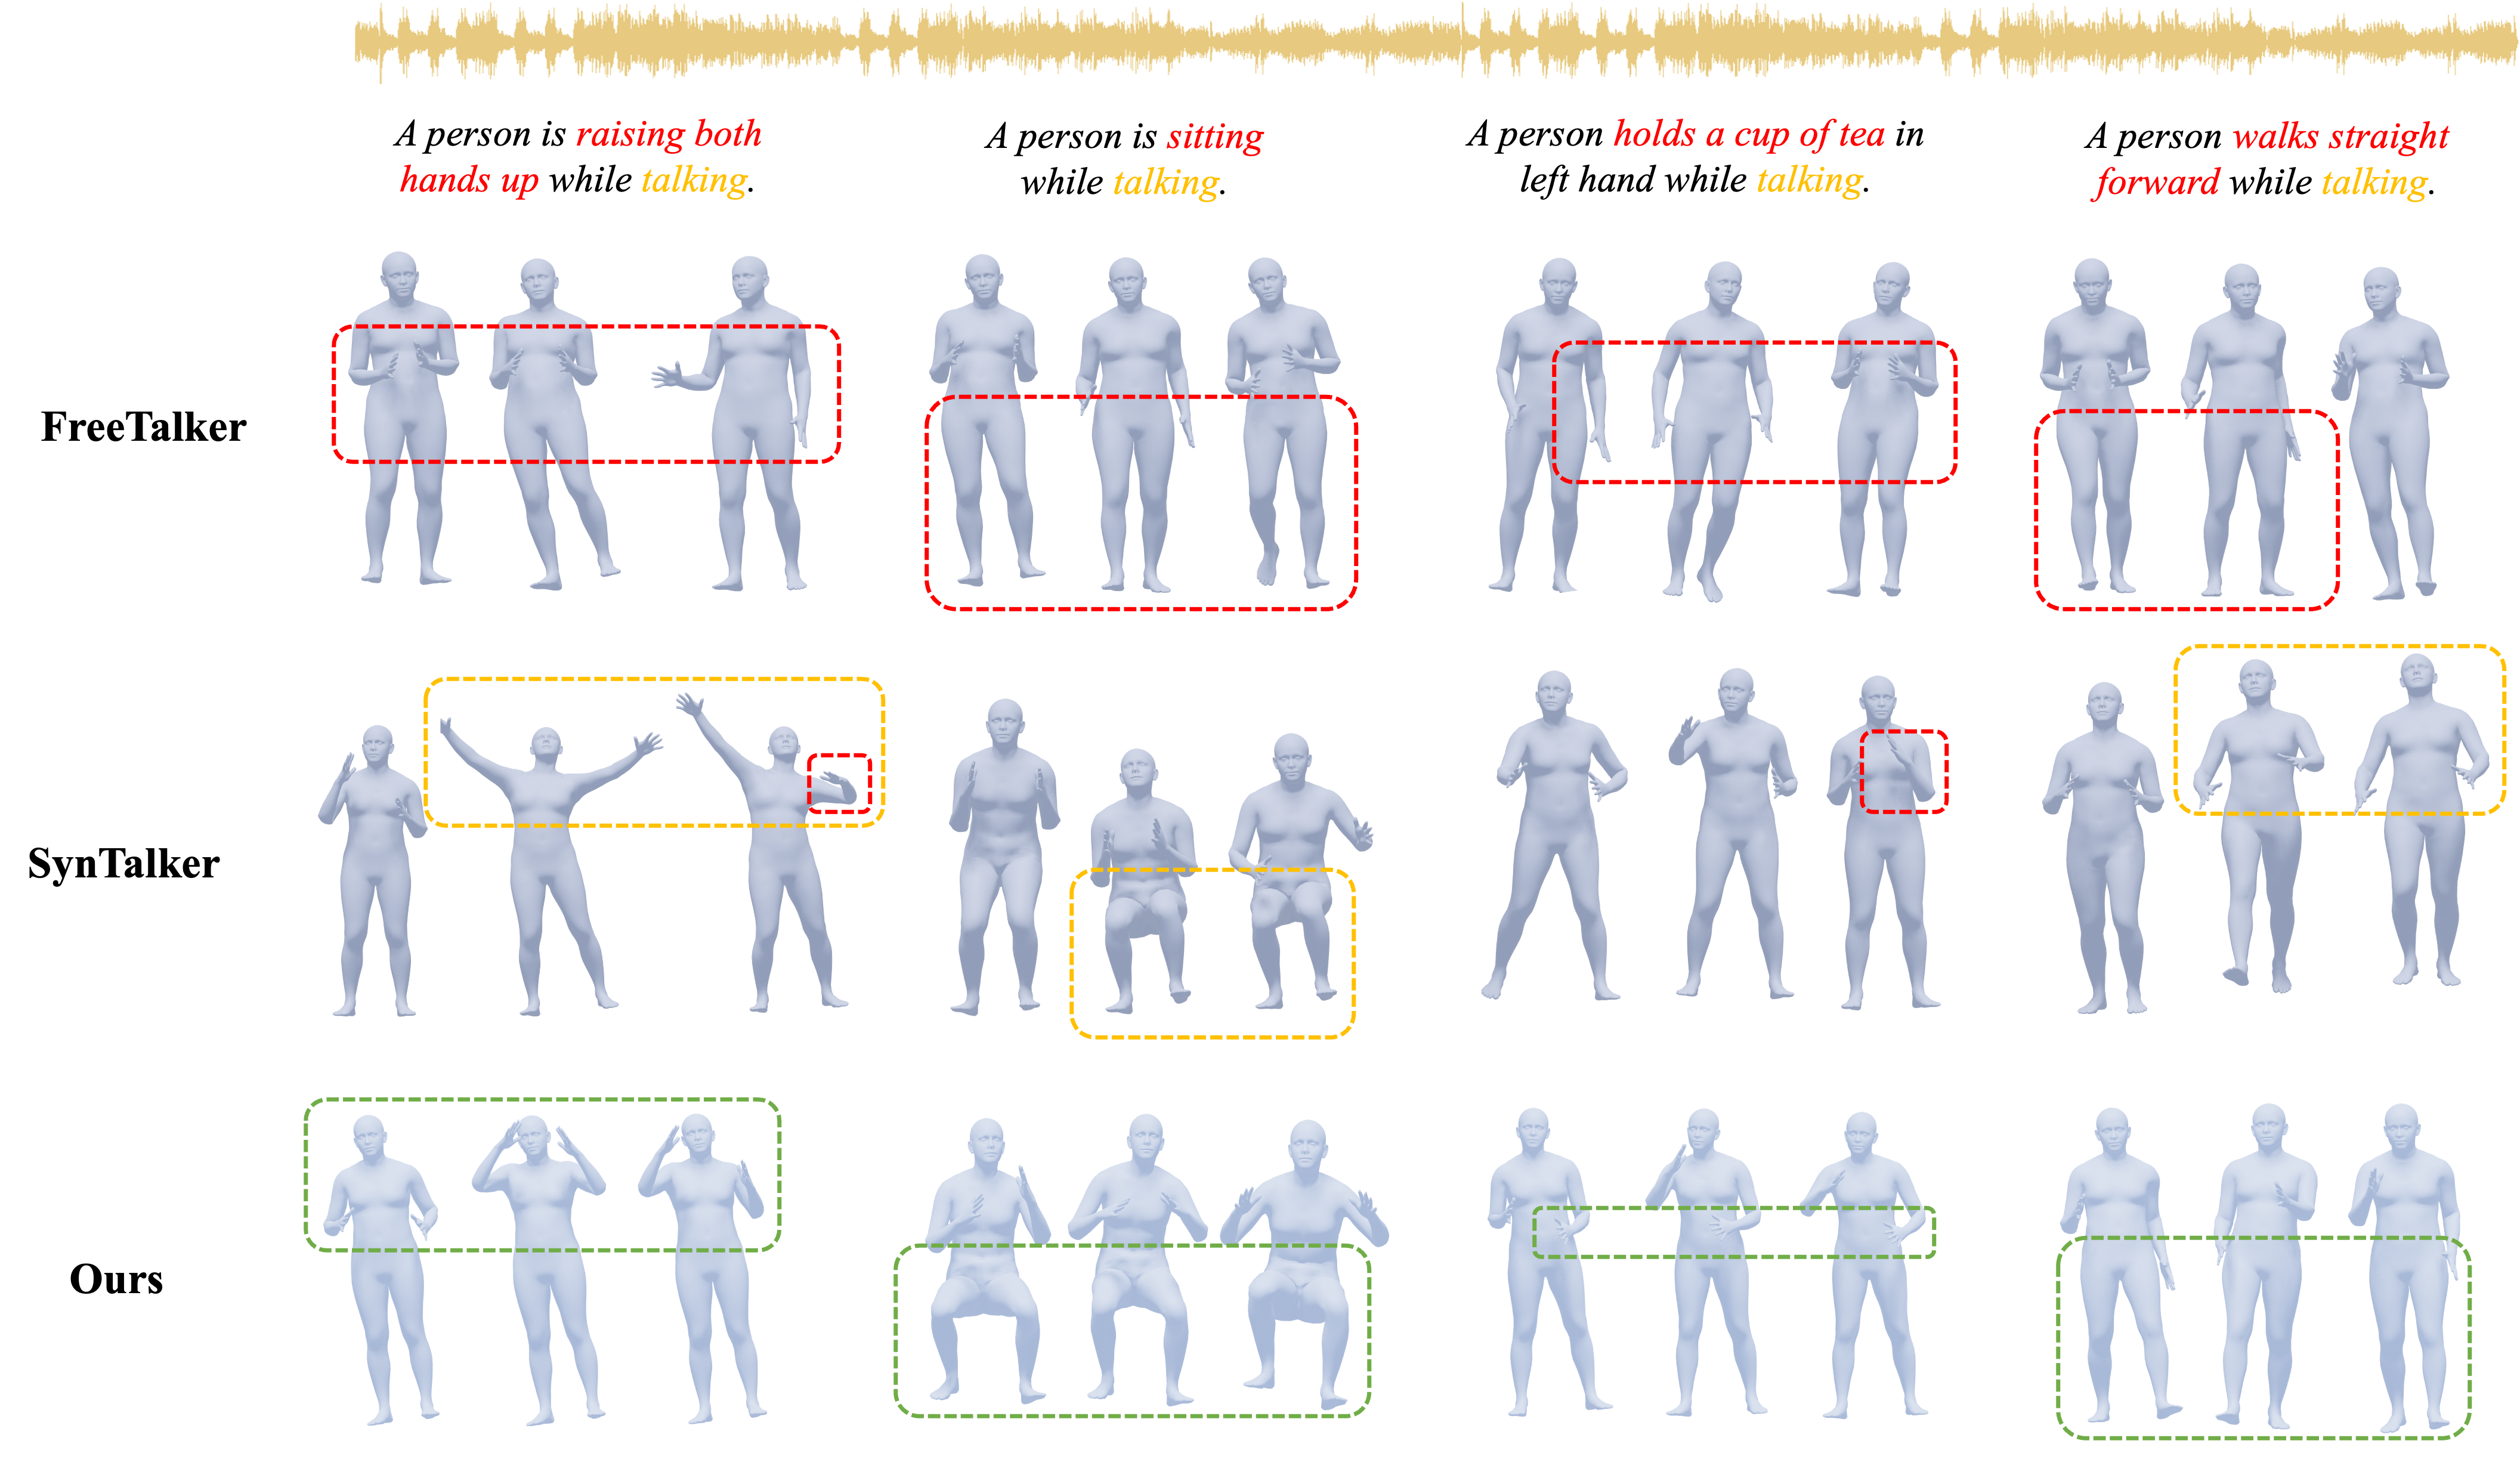
\includegraphics[width=\linewidth]{visualization_v1.png}
  \caption{协同手势生成的定性比较。 \textcolor{red}{红色} 框突出显示语义不一致,\textcolor[RGB]{204,153,0}{黄色} 框表示不自然的动作,\textcolor[RGB]{34,139,34}{绿色} 框表示协同良好的自然手势。}
  \label{fig:method:visualization}
\end{figure*}


\subsection{协同手势生成}
\subsubsection{定性对比}
本文首先评估本文的方法在生成协同的语音同步、语义相关的运动方面的表现。
如图~\ref{fig:method:visualization} 所示,本文将其与仅有的两部作品~\cite{yang2024freetalker,chen2024syntalker} 进行了比较,这两部作品都涉及相关的协同生成任务。
参照~\cite{chen2024syntalker},本文使用语音输入和四种不同的文本描述展示结果:\textit{``raising both hands up''}、\textit{``sitting''}、\textit{``holds a cup of tea''}和\textit{``walks straight forward''}。
结果表明,本文的方法有效地产生了节奏一致且语义一致的协同手势,同时实现了更自然的外观。
相比之下,FreeTalker 无法生成语义动作,而仅专注于语音驱动的手势。虽然 SynTalker 实现了一定的协同性,但它表现出细节上的不一致和不自然的僵硬性。
例如,在传达\textit{``holding ... in left hand''}时,本文的方法指示说话者将左手保持在腰部附近的稳定位置,这是FreeTalker和SynTalker结果中都缺失的细节。在表达\textit{``raising both hands up''}时,本文的方法通过同时抬起双臂保持与文本的一致性,而FreeTalker未能抬起双手,SynTalker则在举起后放下一只手。
此外,在表现\textit{``sitting''}和\textit{``walking straight forward''}时,本文的方法生成了更自然的说话者动作,相比之下SynTalker的结果显得较为僵硬。
值得注意的是,与 SynTalker 不同,本文的方法不需要额外的预训练或推理成本,并且可以实现更快的推理,如第~\ref{sec:exp_ablation}节所示。



% 主结果
\begin{table*}[t]
  \centering
  \setlength{\tabcolsep}{2pt}  % 添加这一行
  \caption{与基线模型和消融研究进行比较的定量结果。`$\rightarrow$' 表示越接近真实运动越好。每个指标均在 20 次运行的 95\% 置信区间下报告。本文报告 BC $\times 10^{-1}$ 和 Top-1 R-Precision。}
    % \small
    \footnotesize
    \label{tab:main_results}
    \begin{tabular}{c c@{\hspace{3pt}} c@{\hspace{3pt}} c@{\hspace{3pt}} c@{\hspace{3pt}} c@{\hspace{3pt}} c@{\hspace{3pt}} c@{\hspace{3pt}} c@{\hspace{3pt}} c}
    \toprule
    \multirow{3}{*}{Methods} & \multicolumn{2}{c}{Reconstruction} & \multicolumn{3}{c}{Audio-to-Gesture} & \multicolumn{4}{c}{Text-to-Motion} \\
    \cmidrule(lr){2-3} \cmidrule(lr){4-6} \cmidrule(lr){7-10}
    & Jerk$\rightarrow$ & Accel.$\rightarrow$ & FGD$\downarrow$ & BC$\uparrow$ & L1Div$\uparrow$ & FID$\downarrow$ & MM-Dist$\downarrow$ & Div$\rightarrow$ & R-Precision$\uparrow$ \\
    \midrule
    GT & $1.165^{\pm .000}$ & $0.043^{\pm .000}$ & - & - & - & - & $6.205^{\pm .043}$ & $5.512^{\pm .114}$ & $0.140^{\pm .008}$ \\
    Freetalker~\cite{yang2024freetalker} & $0.611^{\pm .013}$ & $0.030^{\pm .000}$ & $2.101^{\pm .026}$ & $1.147^{\pm .028}$ & $11.332^{\pm .025}$ & $0.761^{\pm .048}$ & $6.737^{\pm .051}$ & $5.396^{\pm .127}$ & $0.102^{\pm .008}$ \\
    Ours  & $1.190^{\pm .015}$ & $0.039^{\pm .001}$ & $3.173^{\pm .123}$ & $1.327^{\pm .049}$ & $10.861^{\pm .066}$ & $1.118^{\pm .061}$ & $6.814^{\pm .056}$ & $5.558^{\pm .126}$ & $0.100^{\pm .008}$ \\
    Ours-w/o mo. & $1.005^{\pm .014}$ & $0.032^{\pm .000}$ & $2.654^{\pm .041}$ & $2.627^{\pm .043}$ & $19.600^{\pm .089}$ & $3.911^{\pm .163}$ & $7.664^{\pm .050}$ & $4.070^{\pm .117}$ & $0.043^{\pm .004}$ \\
    % Ours-w/o cap. & $1.181^{\pm .011}$ & $0.039^{\pm .000}$ & $2.224^{\pm .074}$ & $2.330^{\pm .060}$ & $12.652^{\pm .109}$ & $1.041^{\pm .042}$ & $6.788^{\pm .056}$ & $5.414^{\pm .133}$ & $0.095^{\pm .008}$ \\
    Ours-w/o hcd.   & $1.201^{\pm .017}$ & $0.038^{\pm .001}$ & $2.302^{\pm .061}$ & $1.910^{\pm .004}$ & $12.781^{\pm .044}$ & $1.260^{\pm .063}$ & $6.872^{\pm .058}$ & $5.303^{\pm .107}$ & $0.102^{\pm .010}$ \\
    Ours-w/o mgc. & $1.239^{\pm .013}$ & $0.039^{\pm .000}$ & $3.123^{\pm .139}$ & $2.256^{\pm .045}$ & $15.363^{\pm .103}$ & $2.568^{\pm .099}$ & $7.031^{\pm .044}$ & $5.447^{\pm .150}$ & $0.082^{\pm .006}$ \\
  \bottomrule
  \end{tabular}
\end{table*}
\subsubsection{定量结果}
由于只有FreeTalker~\cite{yang2024freetalker}和SynTalker~\cite{chen2024syntalker}与本文工作研究范围相似,且SynTalker不支持多模态条件的定量评估方法,因此本文复现FreeTalker作为对比基线。

如表~\ref{tab:main_results}所示,本文的方法在所有评估指标中取得了可比或优越的结果,超过了Freetalker的重建质量,节拍一致性(BC $0.180\uparrow$),多样性(Div $0.162\uparrow$),同时维持有竞争力的文本匹配度。
值得注意的是,这些结果突出了本文方法在保持语音同步和语义相关性之间良好平衡的独特能力,证实了其在生成自然且可控的协同手势方面的有效性。



% 单条件结果 
\begin{table*}[t]
  \centering
  \caption{与 HumanML3D~\cite{guo2022humanml3d} 测试集上的最新方法进行比较。本文按照 \cite{chen2023executing} 计算标准度量。`$\rightarrow$' 表示越接近真实运动越好。每个度量均在 20 次运行的 95\% 置信区间下报告。}
  \label{tab:h3d_results}
  \small
  \begin{tabular}{c cccccc}
  \toprule
  \multirow{2}{*}{Methods} & \multirow{2}{*}{FID$\downarrow$} & \multirow{2}{*}{MM-Dist$\downarrow$} & \multirow{2}{*}{Div$\rightarrow$} & \multicolumn{3}{c}{R-Precision$\uparrow$} \\
  \cmidrule(lr){5-7}
  & & & & Top-1 & Top-2 & Top-3 \\
  \midrule
  GT  &  $0.001^{\pm .001}$ & $3.378^{\pm .007}$ & $10.471^{\pm .083}$ &  $0.490^{\pm .003}$ & $0.682^{\pm .003}$ & $0.783^{\pm .003}$ \\
  MDM~\cite{tevet2022mdm} & $1.390^{\pm .088}$ & $4.599^{\pm .037}$ & $10.704^{\pm .066}$ & $0.363^{\pm .007}$ & $0.553^{\pm .008}$ & $0.662^{\pm .007}$ \\
  T2M-GPT~\cite{zhang2023t2mgpt} &  $0.564^{\pm .012}$ & $3.867^{\pm .008}$ & $10.558^{\pm .083}$  & $0.433^{\pm .003}$ & $0.615^{\pm .002}$ & $0.716^{\pm .003}$ \\
  MLD~\cite{chen2023executing} & $0.963^{\pm .029}$ & $3.898^{\pm .012}$ & $10.401^{\pm .096}$ & $0.429^{\pm .003}$ & $0.613^{\pm .003}$ & $0.717^{\pm .002}$ \\
  MoMask~\cite{guo2024momask} & $0.222^{\pm .007}$ & $3.620^{\pm .011}$ & $10.621^{\pm .096}$ & $0.461^{\pm .002}$ & $0.657^{\pm .003}$ & $0.760^{\pm .002}$ \\
  SynTalker~\cite{chen2024syntalker} & $4.385^{\pm .034}$ & $4.499^{\pm .012}$ & $9.374^{\pm .073}$ & $0.375^{\pm .003}$ & $0.564^{\pm .003}$ & $0.681^{\pm .002}$ \\
  % Ours (w/o mo.rep.) & & & & & \\
  % Ours (w/o cap.)  & & & & &  \\
  % Ours  & $0.540^{\pm .013}$ & $6.833^{\pm .013}$ & $5.672^{\pm .154}$ & $0.104^{\pm .001}$ & $0.191^{\pm .002}$ & $0.270^{\pm .002}$ \\
  Ours  & $0.405^{\pm .012}$ & $3.584^{\pm .012}$ & $9.109^{\pm .235}$  & $0.424^{\pm .003}$ &$0.601^{\pm .003}$ & $0.702^{\pm .003}$ \\
  \bottomrule
  \end{tabular}
\end{table*}

\subsection{文本驱动的运动生成}
\label{sec:exp_t2m}
本文进一步将本文的方法与最先进的文本到运动方法进行比较,以验证其在捕获语义和生成非自发运动方面的能力。
为了公平比较,本文仅使用文本条件报告 HumanML3D 测试集的结果。
表格~\ref{tab:h3d_results} 显示,与 SOTA 模型相比,本文的方法实现了高级性能,实现了最佳文本对齐(MM-Dist 3.584)和第二好的生成保真度(FID 0.405)。这强调了本文的分层控制降噪器在集成细粒度语义方面的有效性。
值得注意的是,本文的方法明显优于类似的协同方法 SynTalker~\cite{chen2024syntalker},突出了其在协同生成和增强语义控制方面的优势。


\begin{figure*}[t]
  \centering
  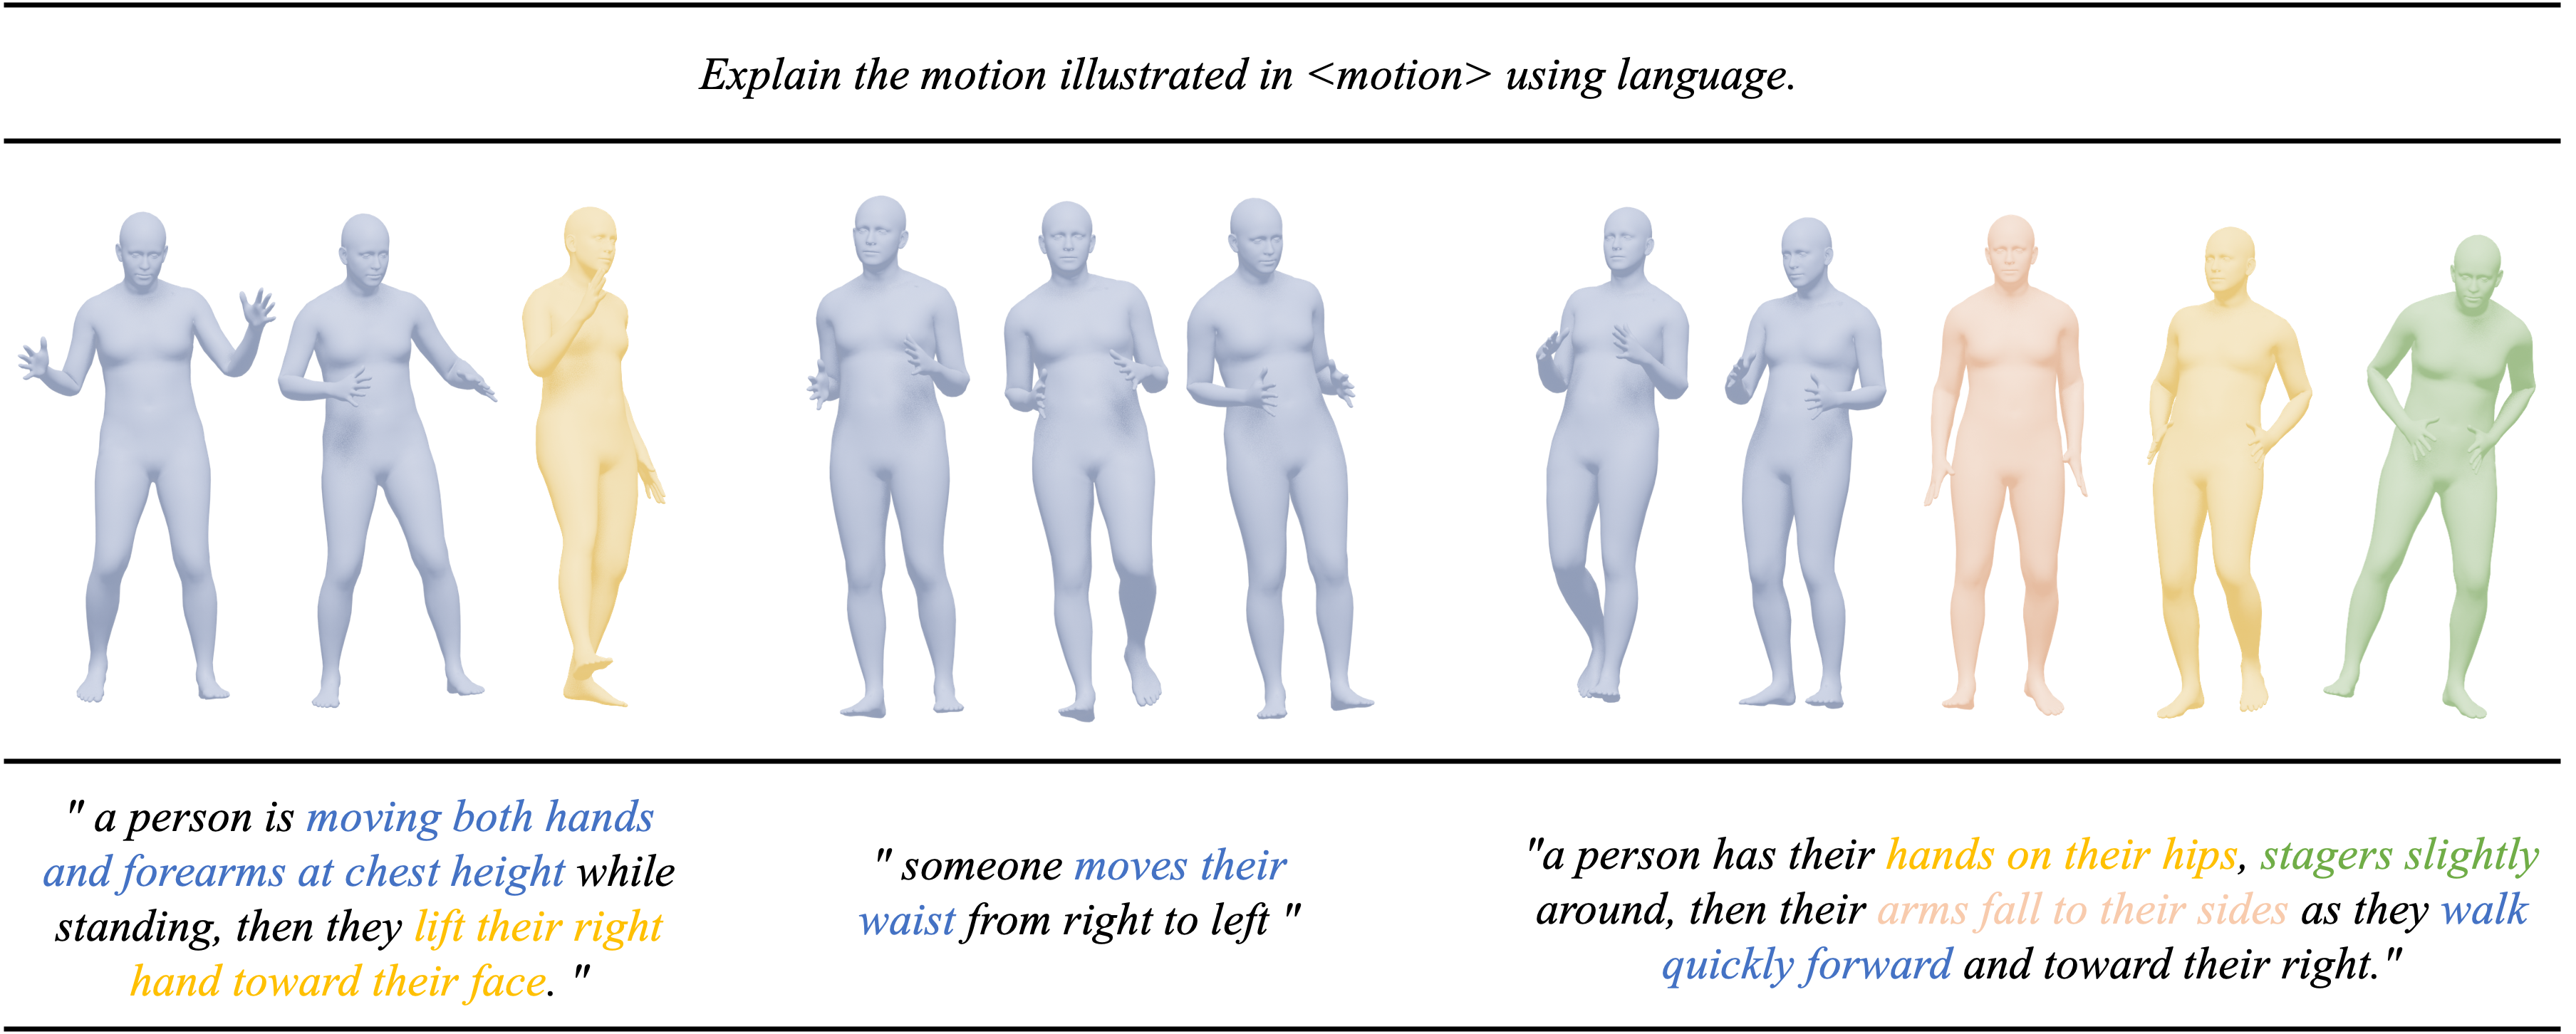
\includegraphics[width=\linewidth]{visualization_caption_v1.png}
  \caption{手势描述生成结果示例。生成的描述准确地描述了整体运动模式和细粒度的手势细节。}
  \label{fig:visualization_caption}
\end{figure*}
\subsection{手势描述生成}
如图~\ref{fig:visualization_caption}所示,所提出的手势描述框架展示了在生成描述性手势标注方面的实用能力。
结果表明,本文的方法不仅能准确描述手势运动分布内的细粒度手部动作(如\textit{``moving both hands and forearms at chest height''}),还能捕捉粗粒度的全身动作(如\textit{``moves their waist from ..."})。
此外,由于手势运动通常持续较长时间,所提出的多粒度描述方法在捕捉长时间窗口内的连续复杂组合动作方面表现出优势(如\textit{``a person \textless motion 1\textgreater, then \textless motion 2\textgreater as \textless motion 3\textgreater''})。
然而,本文也注意到对于较长的手势序列,模型在时序位置感知方面存在困难,偶尔会混淆动作顺序。这一限制可以通过使用本文提出的细粒度描述策略来管理动作复杂度。未来的改进可能涉及引入更强的位置编码或时序建模。

\begin{figure}[t]
    \centering
    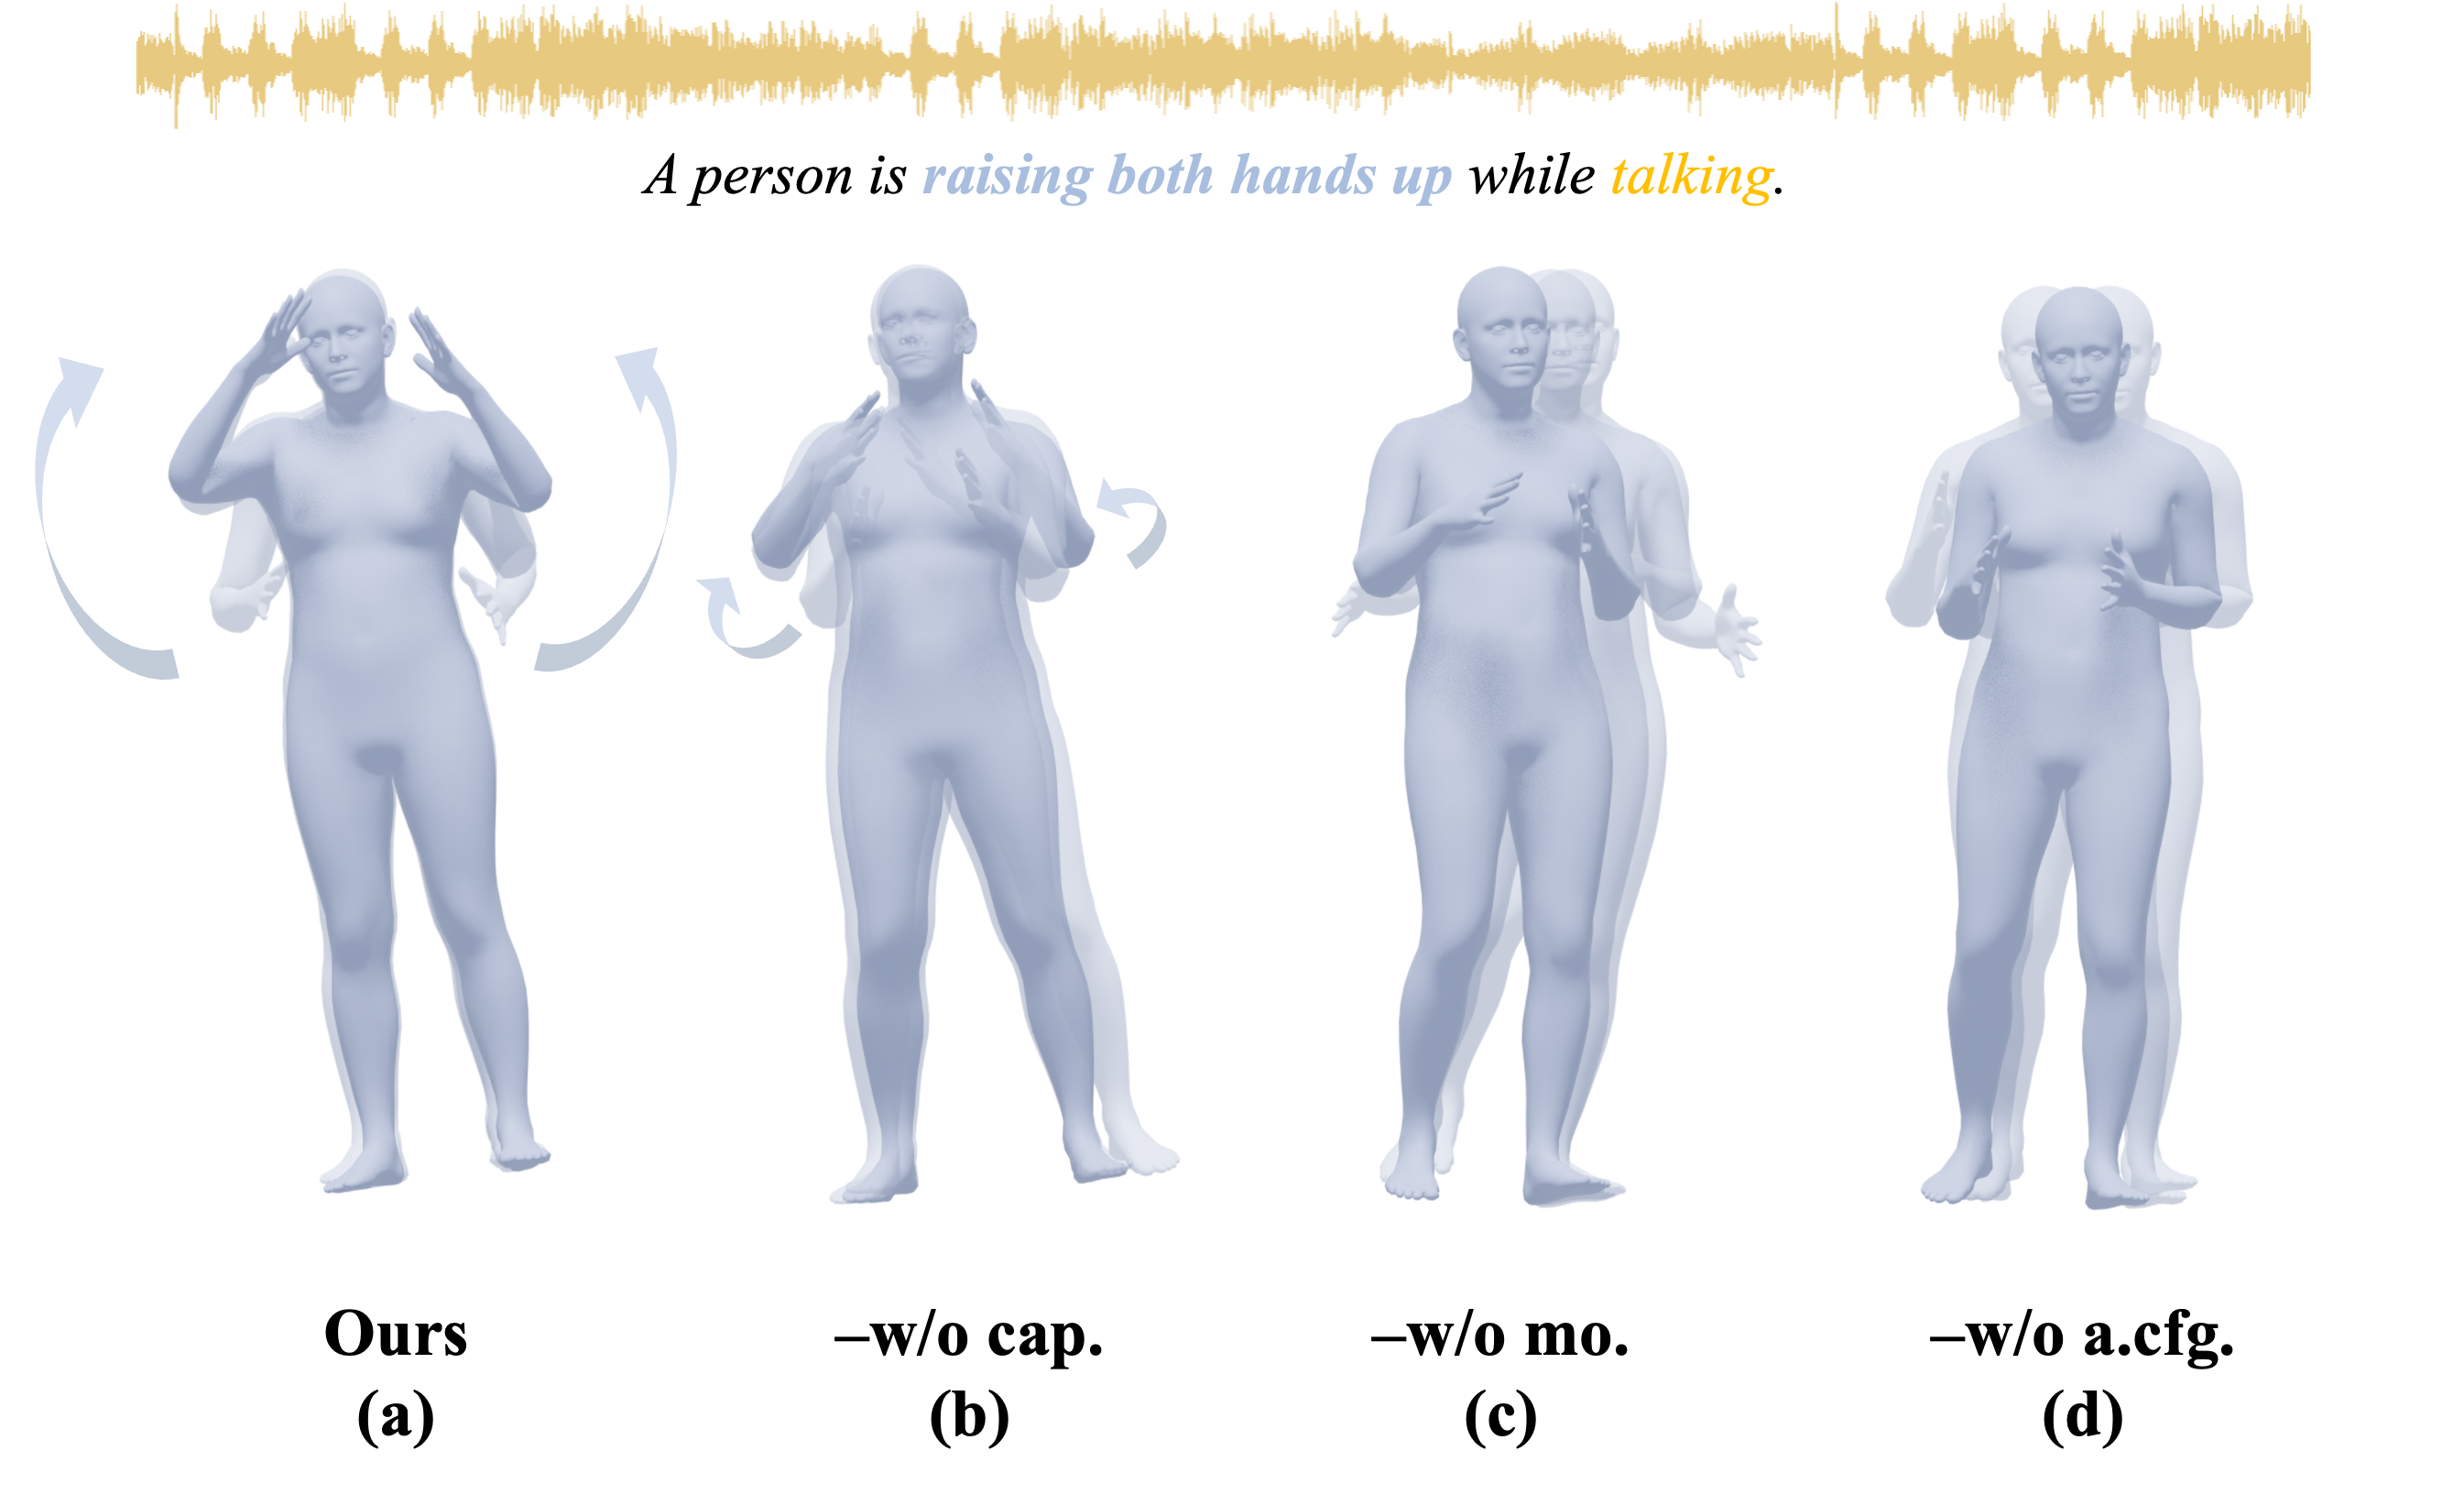
\includegraphics[width=0.7\linewidth]{ablation.png}
    \caption{定性消融研究。结果是使用语音音频和单字幕(“A person is raising both hands up while talking”)生成的。}
    \label{fig:ablation}
\end{figure}

\subsection{消融实验}
\label{sec:exp_ablation}
为了进一步评估不同组件对协同生成的影响,本文在此任务下进行了消融研究。
定量结果如表~\ref{tab:main_results} 所示,定性结果如图~\ref{fig:ablation} 所示。本文使用音频和单个字幕条件 (\textit{``A person is raising both hands up while talking''}) 进行了定性评估。
如图~\ref{fig:ablation}(a) 所示,本文的完整模型有效地捕捉了音频节奏和语义指令,生成自发的语音手势,同时遵循字幕指导产生非自发的手势(向上举起双手)。

\textbf{手势描述。}
图~\ref{fig:ablation}(b)展示了移除手势描述后的影响。没有描述的语义指导,模型只能生成与语音同步的基本协同手势,无法产生有意义的非自发运动。
这表明手势描述在提供语义指导和补充缺失的手势文本标注方面发挥着关键作用。

\textbf{统一运动表示。}
移除统一的运动表征(图\ref{fig:ablation}(c))显著限制了模型生成除典型同语动作之外的多样且语义上有意义的手势的能力。虽然细微的向上手部动作仍然存在,但说话者未能完全执行标题中描述的举起双手的预期手势。
表~\ref{tab:main_results}(\textit{Ours-w/o mo.})中的定量结果进一步证实了这种退化,显示语义相关性大幅下降,反映在明显更差的 FID($2.793\uparrow$)、MM-Dist($0.850\uparrow$)和 R-Precision(Top-1 $0.057\uparrow$)中。

\textbf{分层控制降噪器。} % [定量] 包括denoiser设计,condition集成方式
如表~\ref{tab:main_results}所示,删除分层控制的降噪器(\textit{Ours-w/o hcd.})会导致重建质量下降(Jerk $0.011\uparrow$)和条件协同性减弱。具体而言,该模型表现出更强的偏向于重建同语手势(BC $0.583\uparrow$),同时无法保持语义相关性(MM-Dist $0.058\uparrow$)。这些发现强调了本文的分层控制降噪器在确保有效的多模态条件协同方面的关键作用。

\textbf{多粒度字幕。}
如表~\ref{tab:main_results} 所示,删除多粒度字幕(\textit{Ours-w/o mgc.})会导致生成的手势的语义相关性显著下降。这凸显了本文的多粒度字幕机制在促进精确和上下文感知的语义注入方面的重要性。在这种情况下,音频作为初始条件,而本地字幕提供精细条件。

\textbf{多模态无分类器指导。}
图~\ref{fig:ablation}(d)展示了仅对文本模态应用无分类器指导的效果。
由于训练时缺乏语音模态的无条件指导,模型在推理时难以融合多模态信号,过度依赖语音输入,导致手势多样性有限且语义对齐性差。
这些发现突显了组合多模态指导在实现平衡手势生成中的重要性,有助于整合语音节奏和语义约束。

\begin{table*}[t]
    \centering
    \caption{多粒度字幕策略的消融研究。“Reg.” 表示常规字幕策略,“Dyn.” 表示动态字幕策略,“Hie.” 表示分层字幕策略。
    每个指标均在 20 次运行的 95\% 置信区间下报告。本文报告 BC $\times 10^{-1}$ 和 Top-1 R-Precision。}
    \footnotesize
    \label{tab:ablation}
    \begin{tabular}{c c@{\hspace{3pt}} c@{\hspace{3pt}} c@{\hspace{3pt}} c@{\hspace{3pt}} c@{\hspace{3pt}} c@{\hspace{3pt}} c@{\hspace{3pt}} c@{\hspace{3pt}} c}
    \toprule
    \multirow{3}{*}{Methods} & \multicolumn{2}{c}{Reconstruction} & \multicolumn{3}{c}{Audio-to-Gesture} & \multicolumn{4}{c}{Text-to-Motion} \\
    \cmidrule(lr){2-3} \cmidrule(lr){4-6} \cmidrule(lr){7-10}
    & Jerk$\rightarrow$ & Accel.$\rightarrow$ & FGD$\downarrow$ & BC$\uparrow$ & L1Div$\uparrow$ & FID$\downarrow$ & MM-Dist$\downarrow$ & Div$\rightarrow$ & R-Precision$\uparrow$ \\
    \midrule
    GT & $1.165^{\pm .000}$ & $0.043^{\pm .000}$ & - & - & - & - & $6.205^{\pm .043}$ & $5.512^{\pm .114}$ & $0.140^{\pm .008}$  \\
    Ours-Reg.  & $1.201^{\pm .017}$ & $0.038^{\pm .001}$ & $2.302^{\pm .061}$ & $1.910^{\pm .004}$ & $12.781^{\pm .044}$ & $1.260^{\pm .063}$ & $6.872^{\pm .058}$ & $5.303^{\pm .107}$ & $0.102^{\pm .010}$  \\
    Ours-Dyn.  & $1.189^{\pm .013}$ & $0.038^{\pm .000}$ & $2.866^{\pm .106}$ & $1.943^{\pm .037}$ & $14.471^{\pm .110}$ & $1.404^{\pm .049}$ & $6.955^{\pm .044}$ & $5.440^{\pm .114}$ & $0.095^{\pm .006}$  \\
    Ours-Hie.  & $1.190^{\pm .015}$ & $0.039^{\pm .001}$ & $3.173^{\pm .123}$ & $1.327^{\pm .049}$ & $10.861^{\pm .066}$ & $1.118^{\pm .061}$ & $6.814^{\pm .056}$ & $5.558^{\pm .126}$ & $0.100^{\pm .008}$ \\
    \bottomrule
    \end{tabular}
\end{table*}

\textbf{多粒度描述控制。}
表~\ref{tab:ablation}进一步展示了本文方法在不同粒度描述控制策略下的性能。
分层控制策略(分层控制)在所有指标上实现了最优平衡:与常规和动态控制策略相比,它表现出更好的语义相关性(MM-Dist更低,$6.814$ vs $6.872$和$6.955$)、更好的运动质量(FID降低11.3\%和25.6\%),同时有效维持了语音同步性和运动多样性。
此外,动态策略在协同手势同步性(BC: $1.943$)和多样性(L1Div: $14.471$)方面表现出优势,这可能归因于其自适应采样机制增强了训练数据的多样性,使模型能够产生更丰富的节奏手势模式。
这些综合结果表明,本文的多粒度描述控制策略有效协同了多模态信号,在运动自然度、语音同步性和语义对齐性之间实现了平衡的权衡。分层控制策略在细粒度语义注入方面表现尤为出色,导致生成手势具有更强的语义相关性。

\textbf{推理时间。}
尽管扩散模型表现出色,但其较长的推理时间仍是主要瓶颈。
为评估推理效率,本文在单个NVIDIA RTX 3090 GPU上测量每句平均推理时间(AITS)~\cite{chen2023executing},批量大小设为1,不包括模型加载时间。
结果显示本文的方法实现了 $0.842^{\pm .002}$ 秒的AITS,比FreeTalker~\cite{yang2024freetalker} ($6.632^{\pm .044}$s) 和 SynTalker~\cite{chen2024syntalker} ($5.804^{\pm .044}$s) 快6倍以上。
这种显著的加速可以归因于本文高效的分层去噪架构和优化的潜在扩散过程,使本文的方法更适合实际应用。

\subsection{更多可视化结果}
\textbf{更多协同生成结果。}
如图~\ref{fig:vis_supply}所示,本文使用相同的音频和不同的文本标题提供了更加协同的生成结果。
这些结果进一步证实了本文提出的方法在联合语音字幕控制下生成协同语音自发手势和字幕驱动的非自发运动的有效性。

% 更多手势字幕结果
\textbf{更多手势字幕结果。}
本文在图~\ref{fig:vis_caption_supply}中展示了额外的手势字幕结果,进一步证明了本文的方法在准确地将手势映射到文本方面的有效性。
正如彩色框中突出显示的那样,该模型在描述复杂、连续的动作时成功捕捉了细粒度的手部动作和粗粒度的全身动作。

\begin{figure*}[t]
  \centering
  \includegraphics[width=\linewidth]{visualization_supply.png}
  \caption{协同手势生成的更多视觉结果。}
  \label{fig:vis_supply}
\end{figure*}

\begin{figure*}[t]
  \centering
  \includegraphics[width=\linewidth]{visualization_caption_supply.png}
  \caption{更多手势字幕结果。彩色框突出显示了手势和文本字幕之间的精确映射。}
  \label{fig:vis_caption_supply}
\end{figure*}


\section{本章小结}
针对手语教学中标准示范资源缺乏的问题,本章提出了一种基于描述驱动的协同手势生成框架(CoordSpeaker),旨在解决手势生成中的语义标注缺失和多模态协同控制挑战。
首先,第~\ref{sec:method:m_rep}节引入了统一的运动表示方法,通过将不同来源的运动数据映射到紧凑的潜在空间,为跨数据集手势生成奠定基础。
随后,第~\ref{sec:method:gld}节提出了可控手势潜在扩散模型,该模型通过手势VAE学习紧凑的潜在表示,并利用分层条件扩散模型实现高效的多模态条件生成。
为了解决手势数据缺乏描述性文本标注的问题,第~\ref{sec:method:caption}节设计了一个手势描述框架,利用动作-语言模型为手势数据生成语义标注。
第~\ref{sec:method:control}节提出的多粒度描述控制机制进一步增强了对生成过程的精确控制。
最后,第~\ref{sec:experiments}节通过大量定性与定量实验验证了本文方法的有效性。
大量实验表明,本文方法不仅能生成语义连贯、节奏同步的协同手势动作,而且在推理效率上相比现有方法提升了6倍以上,为手语标准示范动作库的扩充奠定了坚实基础。
  % 协同手势生成算法研究
% !TeX root = ../thuthesis-example.tex

\chapter{交互式手语学习助手设计与实现}
手语是听障人士进行交流的主要方式。然而,由于手语学习资源有限、学习成本高等原因,听障人士与普通人之间存在较大的交流障碍。随着人工智能技术的发展,基于多模态的技术为解决这一问题提供了新的可能。然而,手语辅助教学面临两个关键挑战:(1) 手语动作评估困难,缺乏有效的评估机制;(2) 手语标准示范资源缺乏,难以为学习者提供充足的参考样本。

针对上述挑战,本章设计并实现了一个交互式手语学习助手系统。该系统主要包含三个核心功能模块:(1)手语识别模块,基于前文提出的多策略解耦和语义集成网络(MDSI),实现准确的手语动作评估;(2)手语生成模块,基于前文提出的协同手势生成算法(CoordSpeaker),解决标准示范资源不足问题;(3)交互反馈模块,为学习者提供友好的教学指引、实时的动作评估与改进建议。通过这些模块的有机结合,本系统旨在为手语学习者提供高效、智能的学习环境,帮助其掌握规范的手语表达技能、提升手语学习效果。

\section{系统总体设计}

\subsection{设计目标}
本系统旨在通过人工智能技术辅助手语学习过程,为学习者提供实时、准确的动作评估与反馈。系统的核心目标是实现高效的手语学习体验,这要求系统具备实时的动作识别能力和自然的人机交互界面。基于这一目标,系统需要在准确性、实时性、交互性和适应性等多个维度上达到较高水平。
在准确性方面,系统基于本文提出的MDSI算法,通过多模态特征的解耦与融合实现高精度的手语动作识别。该算法能够有效处理手语动作中的细微差异,为学习评估提供可靠的技术支持。
在实时性方面,系统采用并行计算技术,确保手语动作的捕获、识别和反馈过程能够实时完成,从而保证良好的交互体验。
在交互性方面,系统设计了直观的可视化界面,通过实时对比展示标准动作与用户动作的差异,并结合定量评估指标提供针对性的改进建议。在适应性方面,系统支持用户结合学习进度和掌握程度,自主设定练习目标,支持友好、个性化的学习体验。

\subsection{系统架构}
为实现上述设计目标,本系统采用模块化的软件架构设计,如图~\ref{fig:system_arch}所示。系统整体划分为手语识别、手语生成、交互反馈三个核心功能模块,各模块通过统一的消息总线进行通信协作。这种模块化设计不仅提高了系统的可维护性和可扩展性,也便于各个功能模块的独立优化和升级。
手语识别模块作为系统的核心感知单元,负责实时捕获和识别用户的手语动作。该模块基于MDSI算法实现,能够有效处理手语动作中的复杂特征。
手语生成模块则基于CoordSpeaker协同手势生成算法,负责生成标准的手语动作示范,支持基于文本描述的精确控制,为学习者提供准确的参考样本。
交互反馈模块通过比对用户动作与标准动作,实时生成评估结果和改进建议。%该模块采用多维度的评估指标,既关注动作的准确性,也考虑动作的流畅度和节奏感。
% 用户界面模块则通过可视化方式呈现系统功能,提供直观的学习交互体验。


\begin{figure}
    \centering
    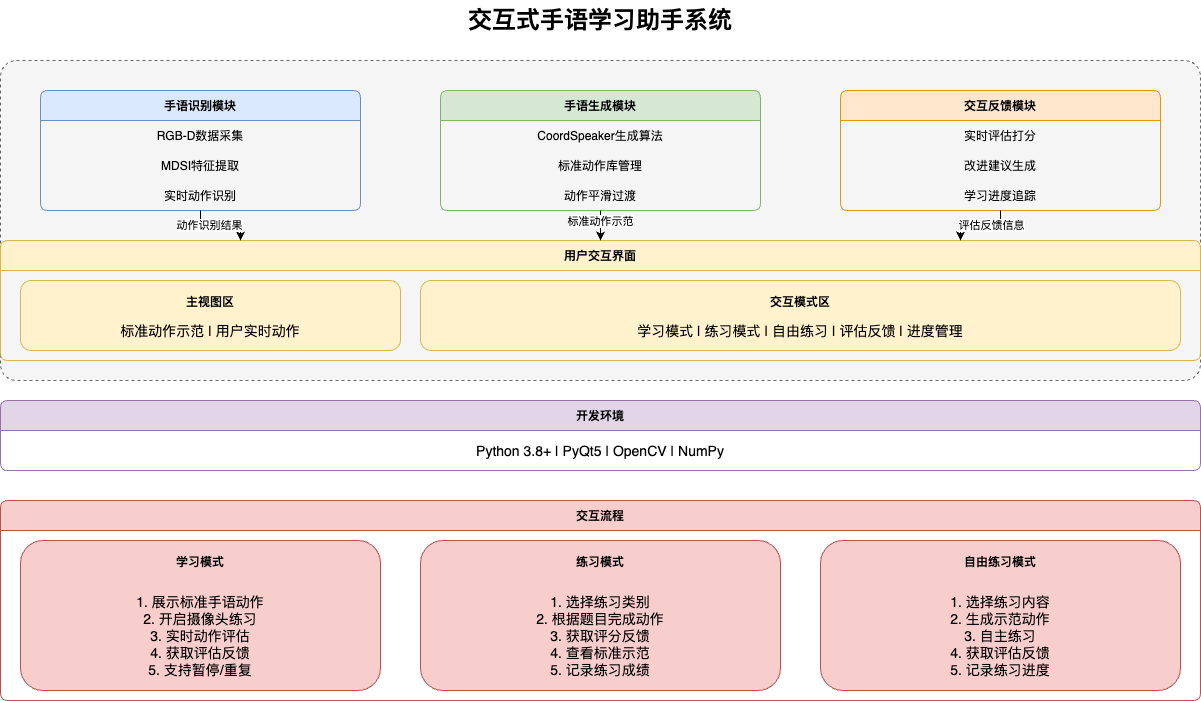
\includegraphics[width=\linewidth]{sys.drawio.png}
    % \caption*{}
    \caption{交互式手语学习助手系统架构}
    \label{fig:system_arch}
  \end{figure}

\section{核心功能模块设计}

\subsection{手语识别模块}
手语识别模块是系统的核心组件之一,负责实时捕获并识别用户的手语动作,进行评估打分。该模块基于第三章提出的MDSI算法,通过RGB-D相机实时采集用户手语动作的RGB图像序列与深度信息。为提升系统实时性能,本模块采用可插拔的高效MDSI算法,基于GPU加速,有效降低了系统延迟。

\subsection{手语生成模块}
手语生成模块负责生成标准手语动作示范,以供学习/练习使用。基于第四章提出的CoordSpeaker协同手势生成算法实现。该模块支持两种工作模式:离线生成模式和实时生成模式。离线生成模式用于预先生成标准动作库,包含常用手语词汇和短语的标准示范动作。实时生成模式则支持根据文本输入即时生成手语动作示范,为用户提供更灵活的学习参考。

\subsection{交互反馈模块}
交互反馈模块通过实时比对用户动作与标准动作,生成评估得分与改进建议。%该模块采用多维度评估体系,包括动作准确度、完整度、流畅度等指标。
系统通过可视化方式直观展示用户动作与标准动作的差异,并结合自然语言描述提供具体的改进建议。此外,模块还会记录用户的学习轨迹,支持学习进度的追踪与分析。


\begin{figure}
    \centering
    \begin{subfigure}[b]{0.7\linewidth}
        \centering
        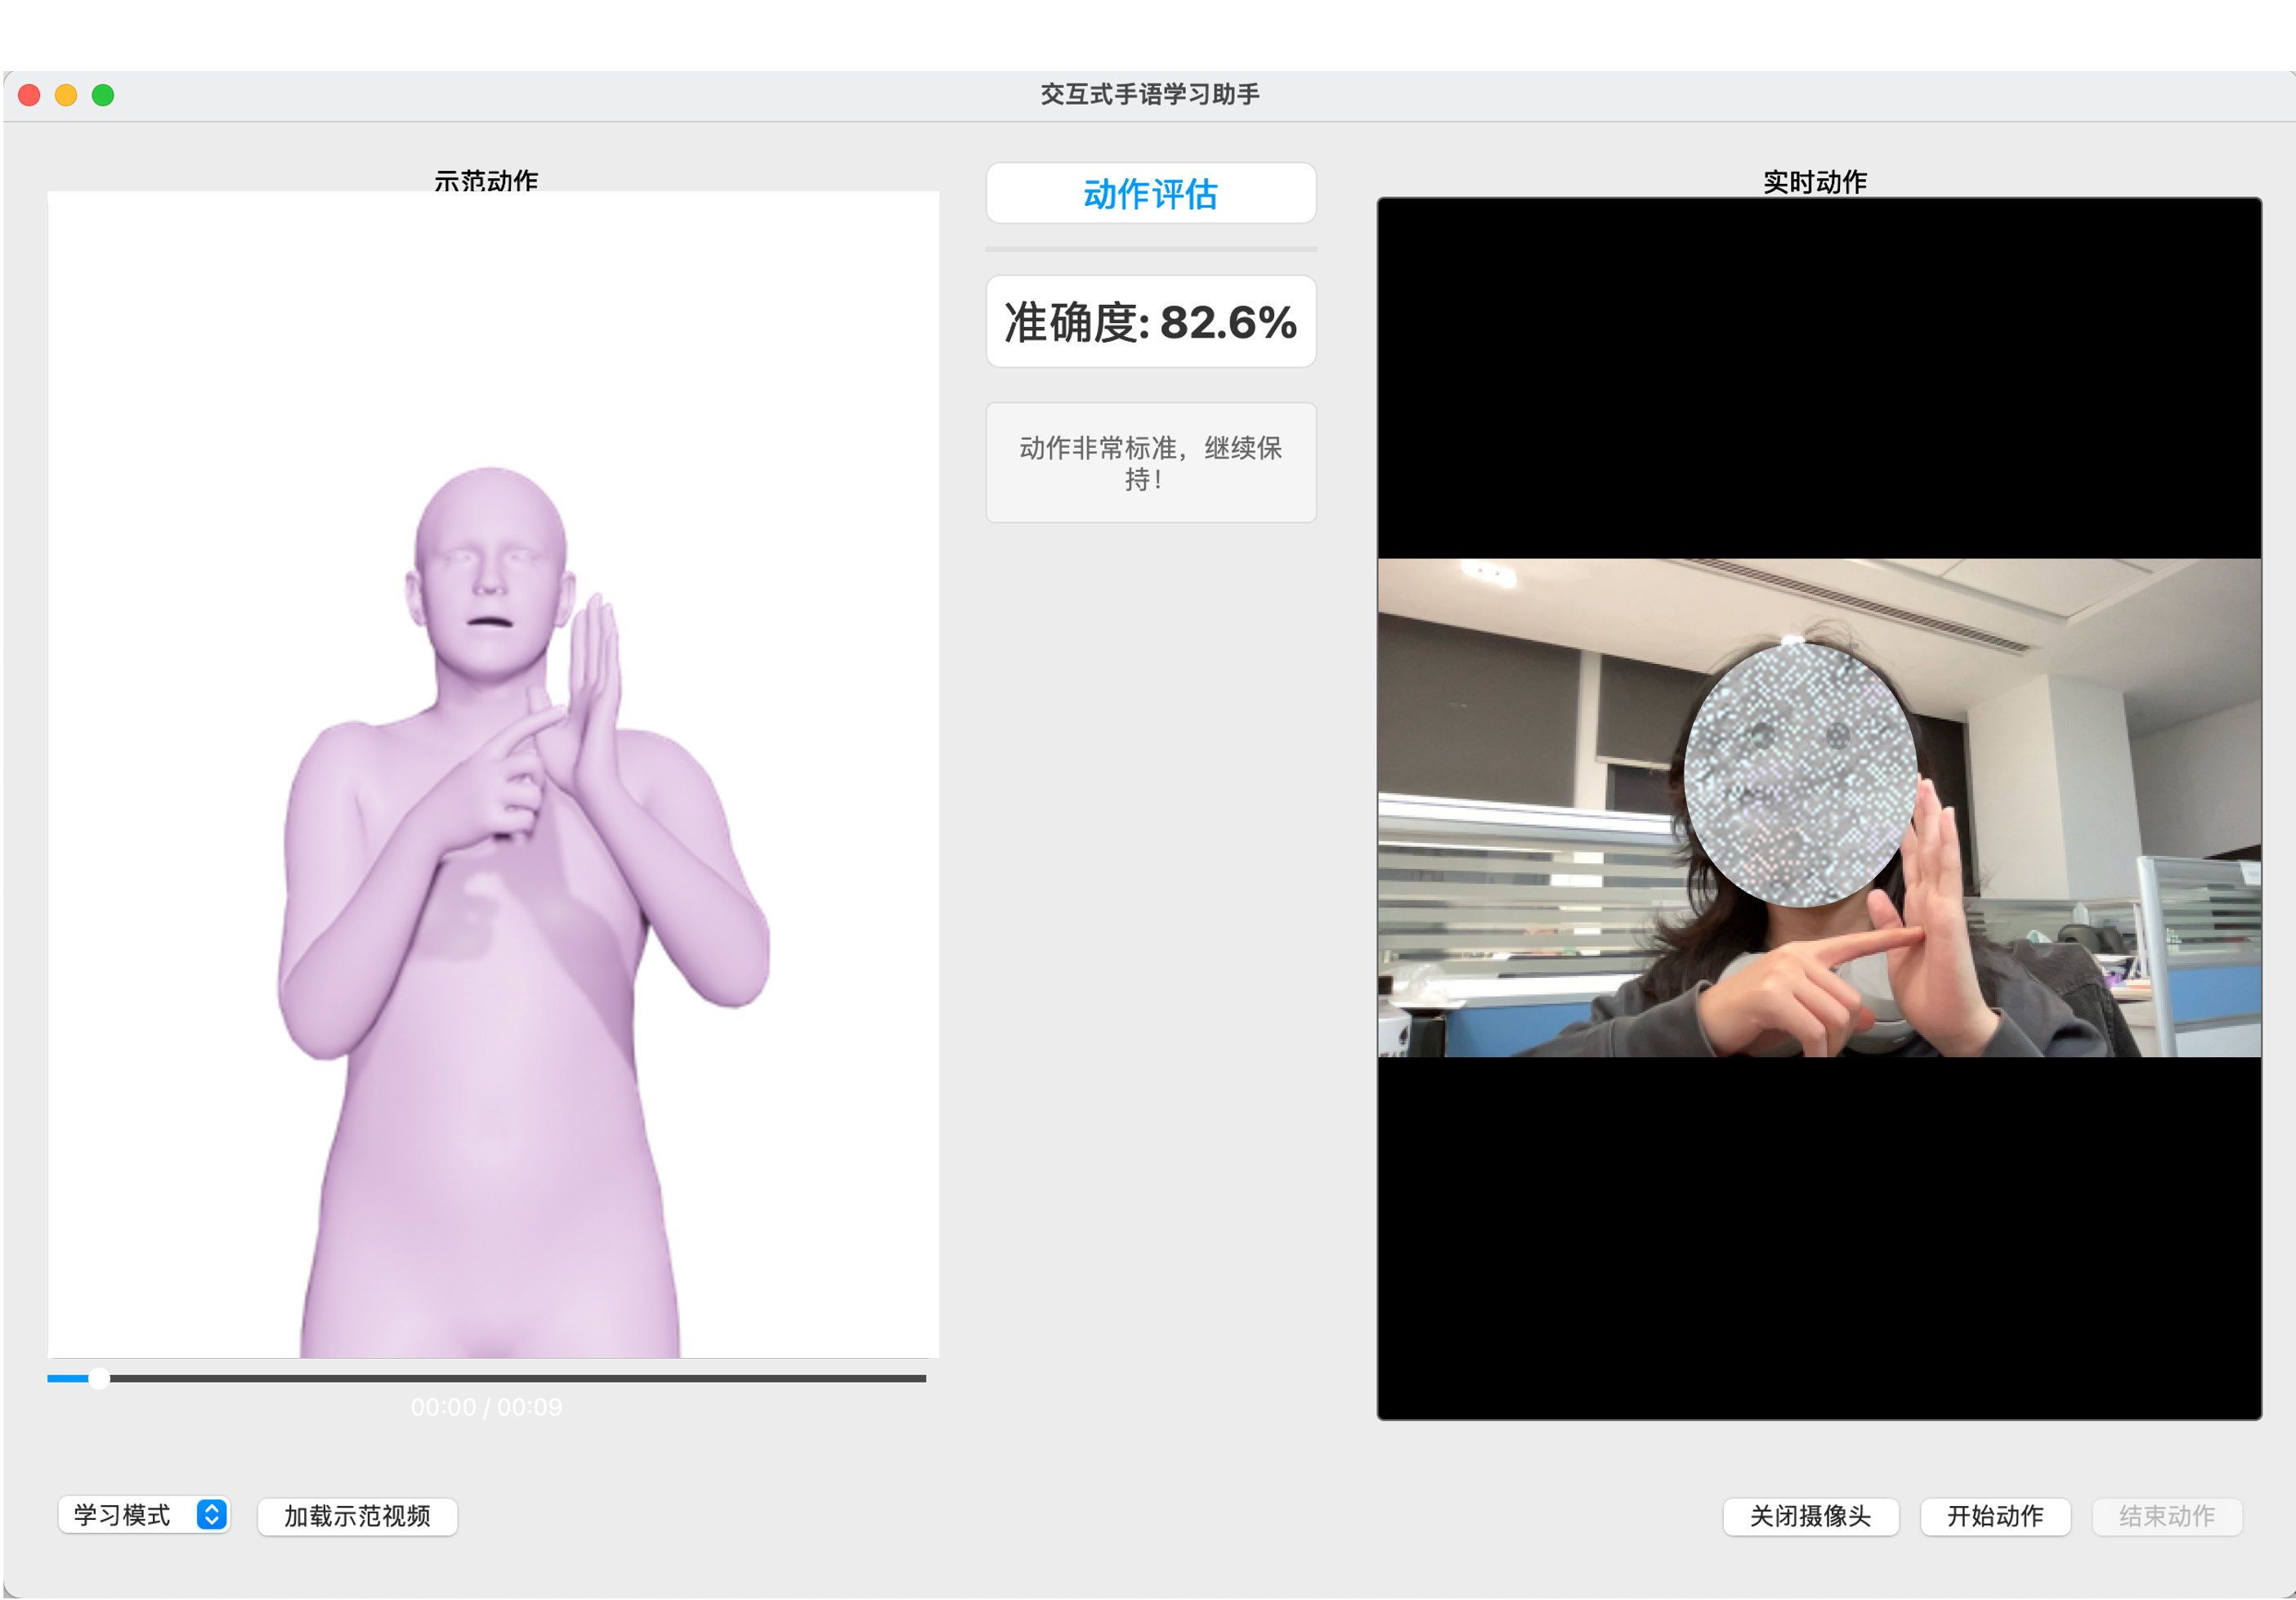
\includegraphics[width=\linewidth]{demo_learn.png}
        \caption{“学习模式”}
    \end{subfigure}
    \hfill
    \begin{subfigure}[b]{0.7\linewidth}
        \centering
        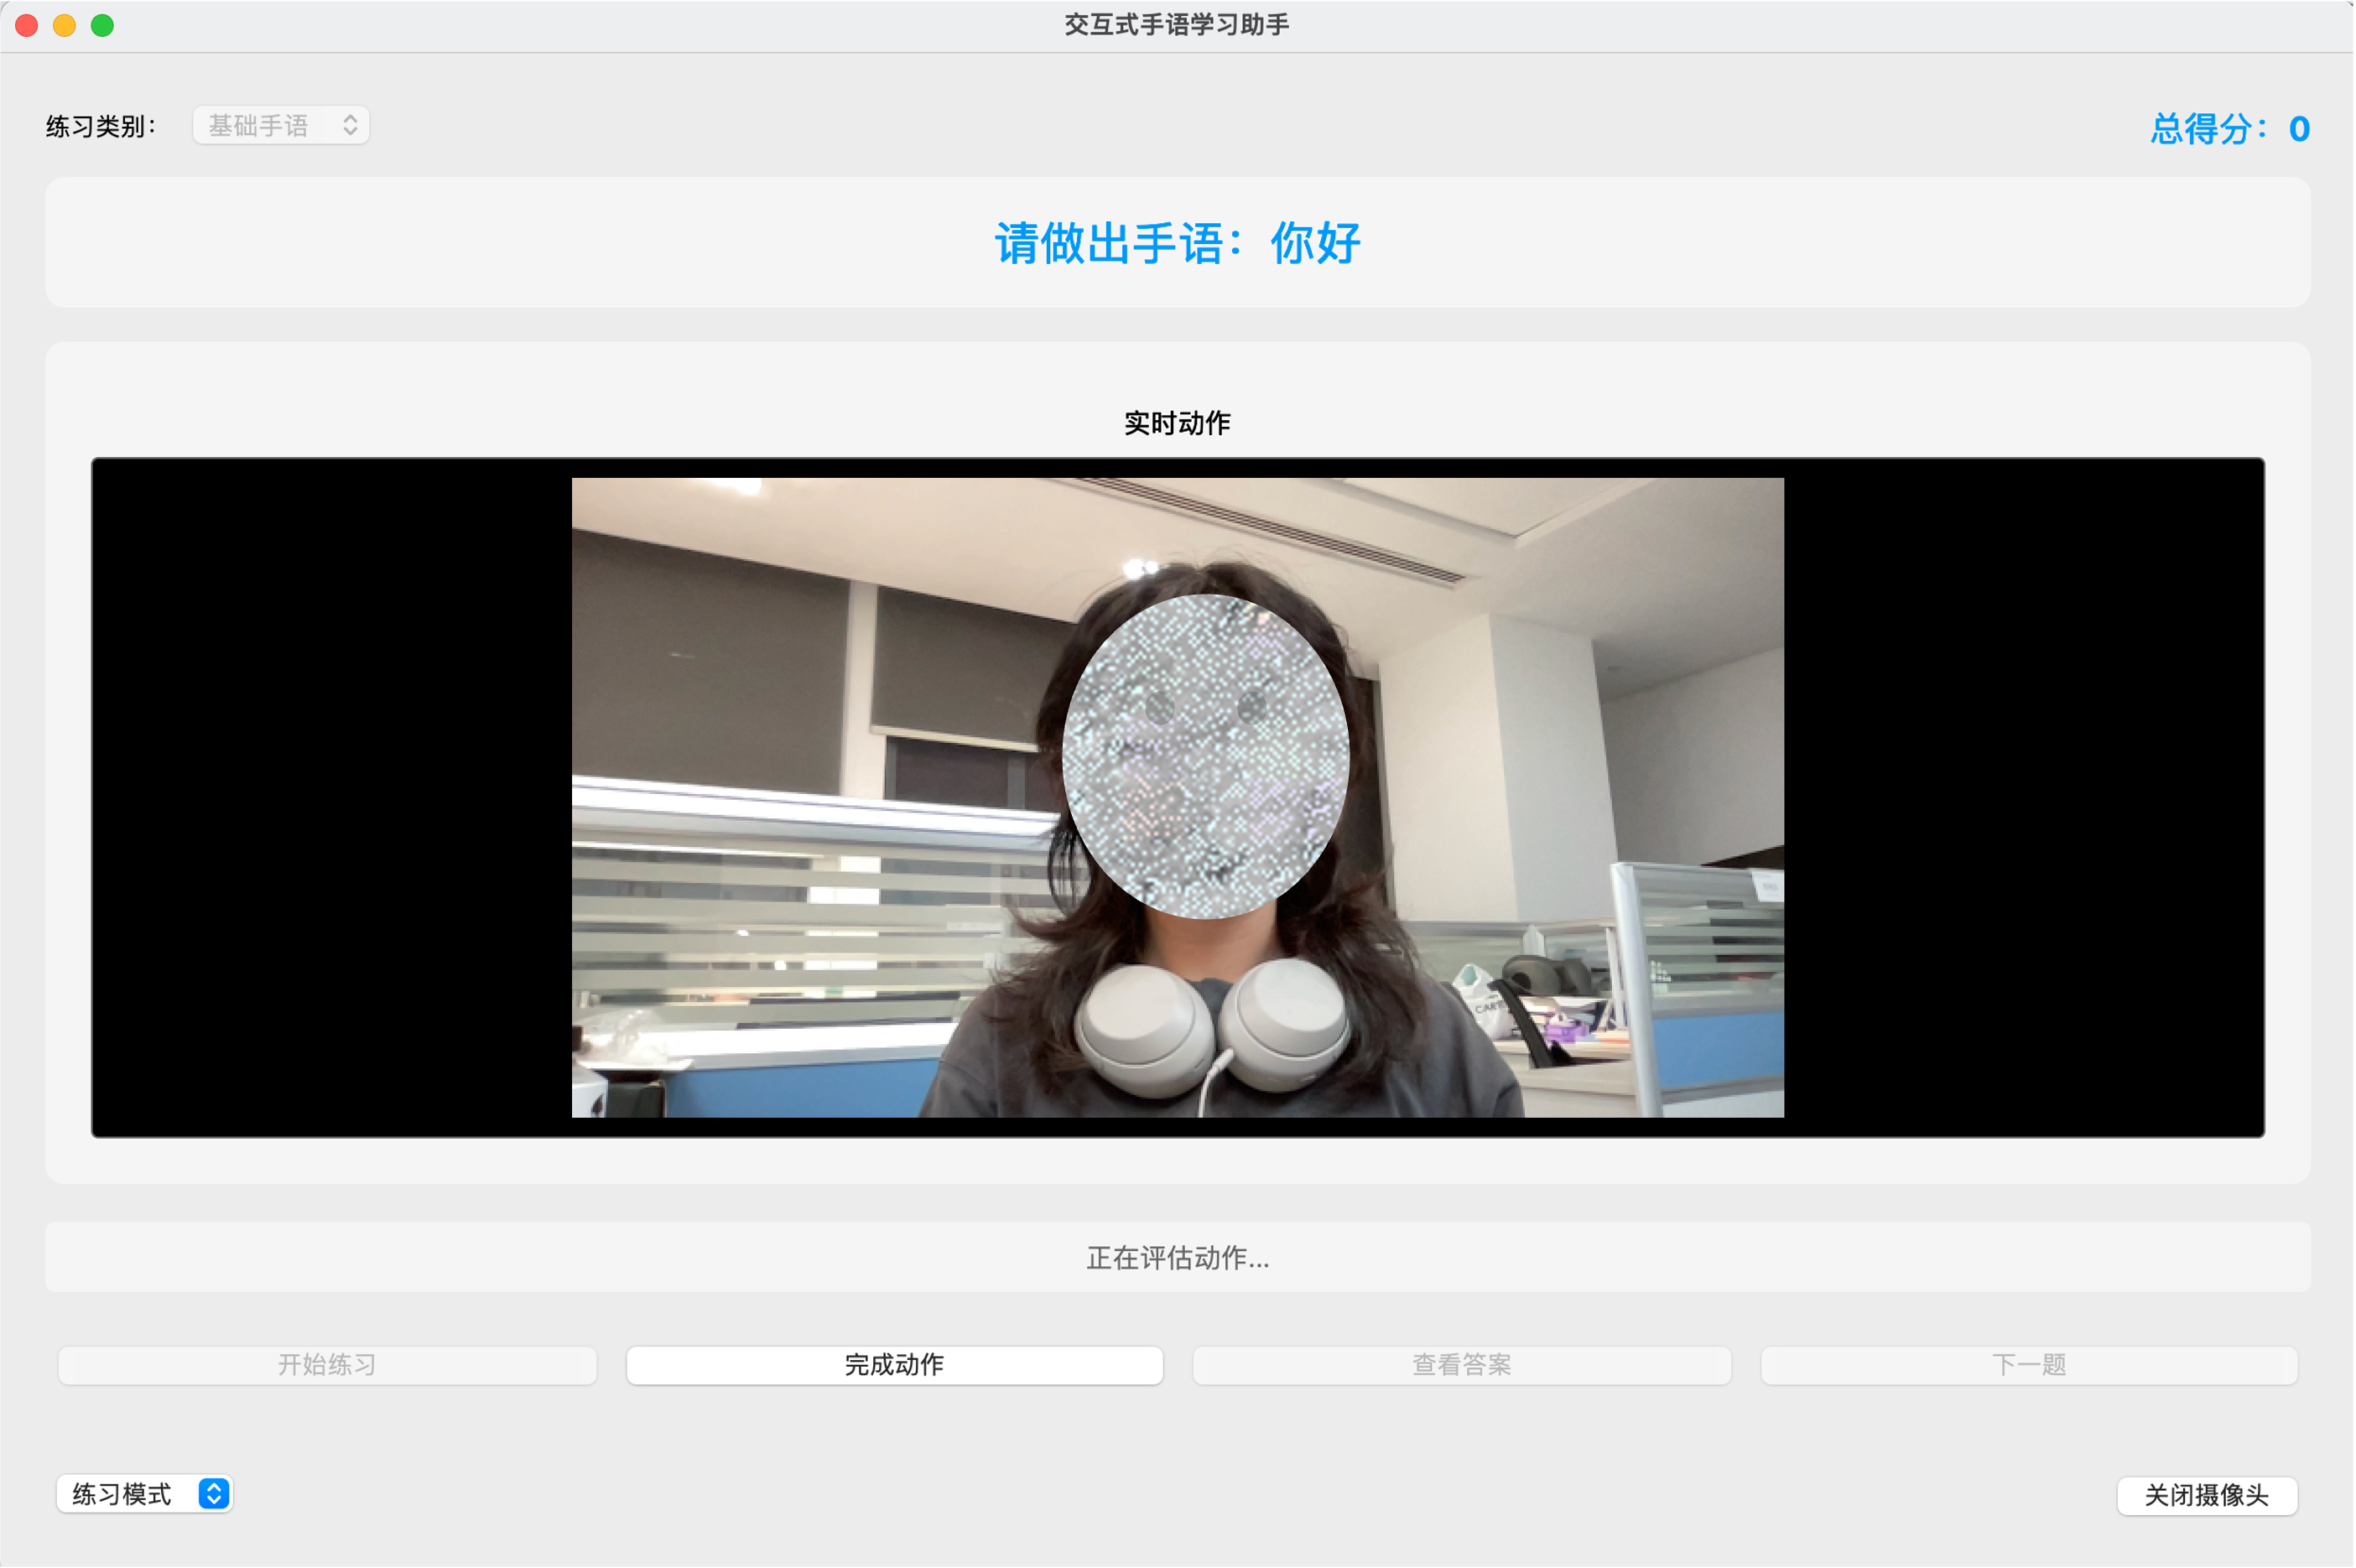
\includegraphics[width=\linewidth]{demo_practice.png}
        \caption{“练习模式”}
    \end{subfigure}
    \caption{用户界面设计。}
    \label{fig:ui_design}
\end{figure}
  
\section{人机交互设计}

\subsection{手语学习模式}
系统支持手语学习、练习评估和自由练习三种主要交互模式。在手语学习模式下,系统首先展示标准手语动作示范,用户通过摄像头采集练习动作,系统实时提供评估反馈。练习评估模式则提供多组不同难度系统化的练习题目,用户需要根据题目完成指定手语动作,系统给出评分和改进建议。自由练习模式支持用户自主选择练习手语词汇,系统生成相应的示范动作,供用户自主练习,并给出评估反馈。

\subsection{用户界面设计}
系统界面采用分区布局设计,主要包含主视图区、评估反馈区和功能控制区三个主要部分。以“学习模式”为例(如图~\ref{fig:ui_design}所示):主视图区采用左右分屏布局,左侧显示标准手语动作示范,右侧实时显示用户的动作画面,便于用户直观对比和模仿。评估反馈区位于界面中部,在用户完成当前手语动作后,显示动作评估分数、关键改进建议和动作要点提示。功能控制区则集中展示学习模式选择、难度调节等操作按钮,保证操作的便捷性。练习模式与学习模式类似,区别在于反馈区位于上下,分别显示题目和评估的分数,用户根据题目完成指定手语动作后,系统给出评分和改进建议,用户可进一步查看答案示范。



\subsection{交互引导设计}
如图~\ref{fig:ui_interaction}所示为帮助用户更好地理解系统功能,系统在主界面及各个模式中设计了交互引导功能。当用户首次启动系统时,会显示可选择的学习模式与系统功能。当首次进入子模式时,系统会通过弹窗提示用户进行相关操作,如开启摄像头,并引导用户进行手语学习。在手语学习过程中,系统支持用户结合掌握程度自主设定学习目标,帮助用户实现持续进步。

\begin{figure}
    \centering
    \begin{subfigure}[b]{0.48\linewidth}
        \centering
        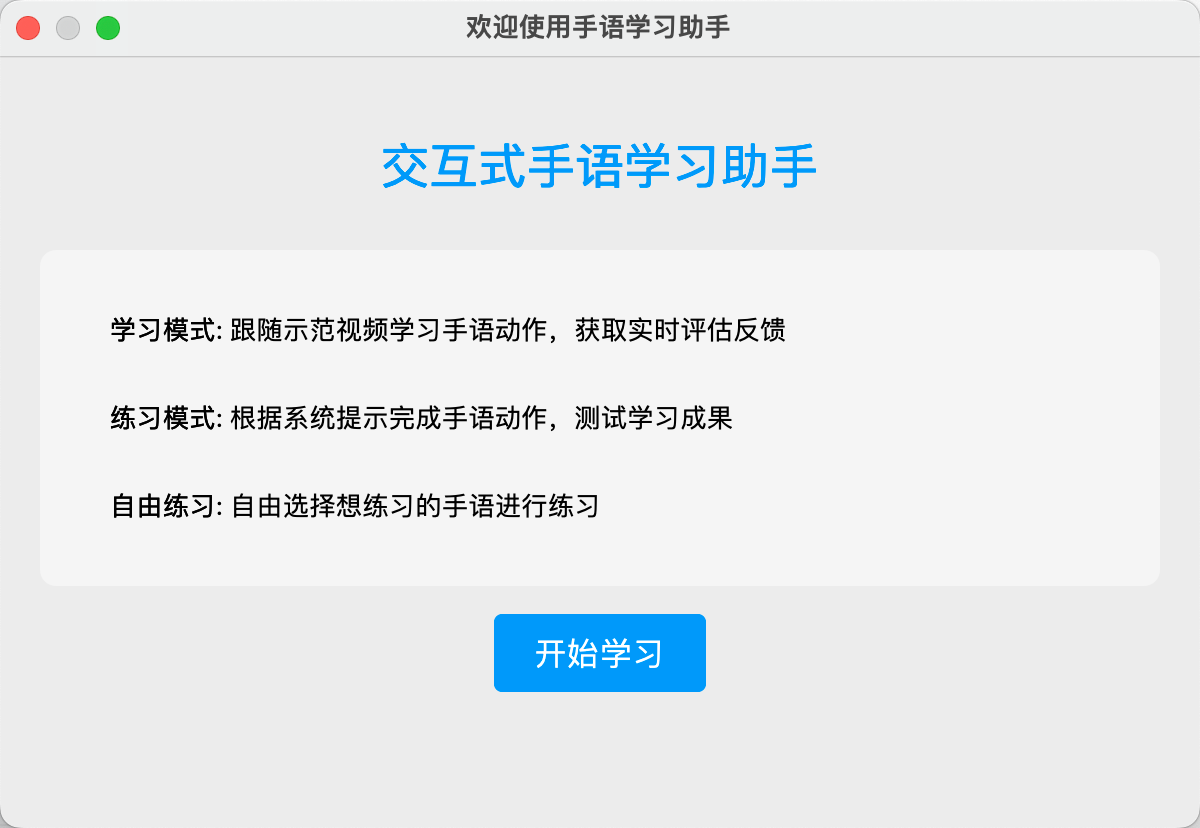
\includegraphics[width=\linewidth]{demo_main.png}
        \caption{“主界面”}
    \end{subfigure}
    \hfill
    \begin{subfigure}[b]{0.48\linewidth}
        \centering
        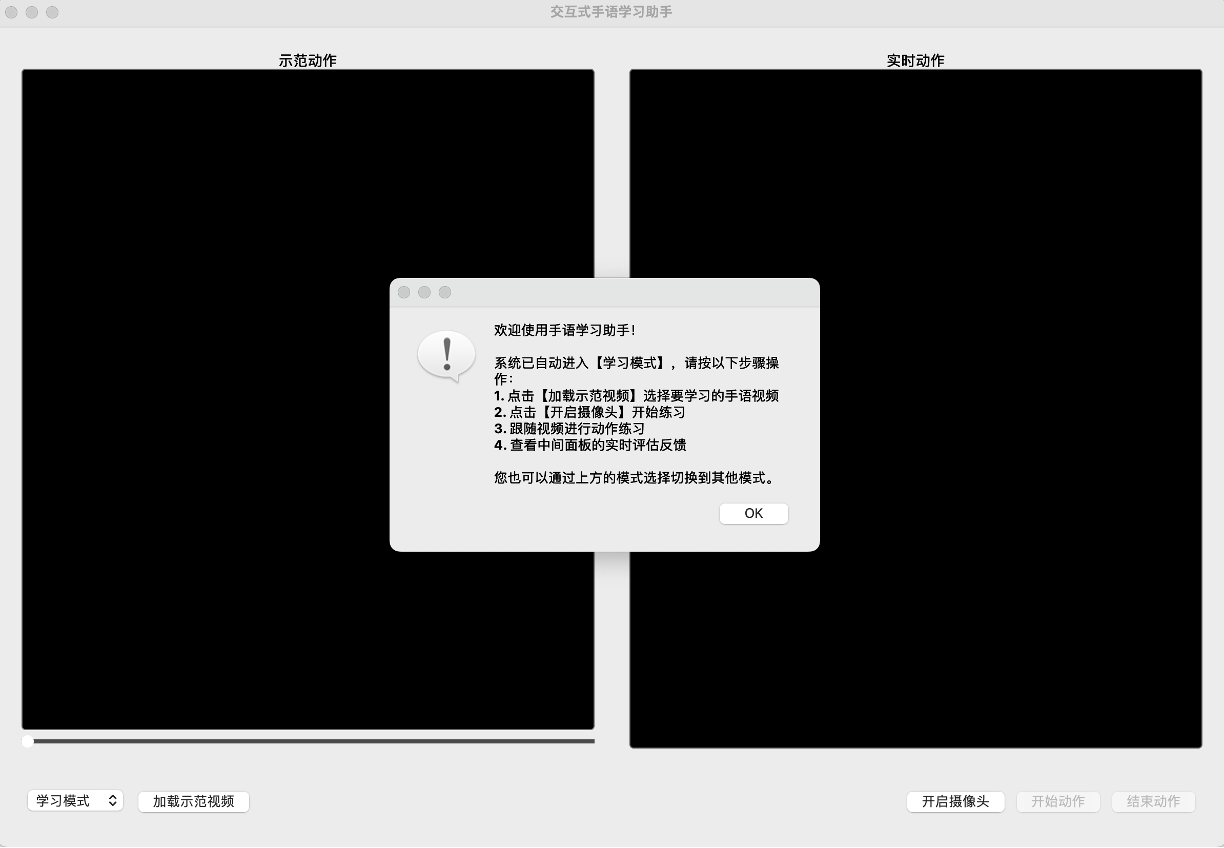
\includegraphics[width=\linewidth]{demo_popup.png}
        \caption{“弹窗引导”}
    \end{subfigure}
    \caption{交互引导设计。}
    \label{fig:ui_interaction}
  \end{figure}

\section{系统实现与部署}
\subsection{开发环境与技术栈}
本系统采用Python作为主要开发语言,基于PyQt5构建图形用户界面。系统的核心算法模块采用PyTorch深度学习框架实现,通过CUDA加速实现GPU并行计算。系统开发环境和主要依赖包括:Python 3.13、PyQt5 5.15、OpenCV 4.11等。
在系统架构方面,采用基于消息队列的模块间通信机制,确保各功能模块之间的解耦与协同。系统部署采用容器化方案,使用Docker实现环境隔离与快速部署。为保证系统的实时性能,手语识别与生成模块均采用GPU加速,并通过多线程技术实现并行执行。

\subsection{关键技术实现}
系统的关键技术实现主要包括以下几个方面:
首先,在手语动作捕获方面,系统通过OpenCV实现RGB-D相机的实时数据采集,采用多线程技术将数据采集与处理解耦,有效降低系统延迟。
其次,在实时手语识别方面,系统基于MDSI算法实现了高效的特征提取与动作识别。
在手语动作生成方面,系统实现了基于CoordSpeaker协同手势生成算法的动作合成引擎。通过预计算与缓存机制,系统显著降低了动作生成的延迟。同时,实现了动作平滑过渡算法,确保生成动作的连贯性与自然性。
在交互反馈方面,系统基于MDSI算法实现了高效准确的手语动作评估,通过分类置信度实时给出评估得分,并基于CoordSpeaker算法生成参考动作答案,同时给出改进建议与学习激励。同时支持学习进度追踪,用户可查看历史学习记录,并根据进度调整学习计划。%设计了基于多特征的评估算法,综合考虑手部位置、运动轨迹、动作速度等因素,实现准确的动作评估。系统采用可视化技术直观展示评估结果,通过骨架对比方式突出动作差异。

    % - 手语识别准确性测试
    % - 手语生成质量评估
    % - 交互响应时间测试
    % - 系统稳定性测试
    % ### 实验设计
    %     - **参与者**:招募10名志愿者,均为手语初学者
    %     - **任务设计**:
    %     1. 基础手语词汇学习(10个常用手语词汇)
    %     2. 简单手语句子练习(5个日常用语)
    %     - **评估指标**:
    %     - 学习效率:完成学习任务所需时间
    %     - 识别准确率:系统识别用户手语动作的准确程度
    %     - 用户满意度:基于问卷的主观评分(1-5分)
    %     - 系统可用性:基于SUS量表的评估


\section{系统测试与评估}
% \subsection{系统功能测试}
% 系统功能测试主要针对手语识别准确性、手语生成质量、交互响应时间和系统稳定性四个方面展开。在手语识别准确性测试中,本文采用标准测试集评估系统的识别性能。测试结果表明,\textcolor{red}{系统在10类常用手语词汇识别任务上达到了99\%以上的准确率。}
% 在手语生成质量评估中,\textcolor{red}{本文邀请专业手语教师对系统生成的标准动作进行评估。评估结果显示,系统生成的手语动作在准确性、流畅性和自然度方面均获得了较高评价。}
% 交互响应时间测试结果表明,\textcolor{red}{系统的端到端延迟控制在100ms以内,满足实时交互需求。}
% 系统稳定性测试采用持续运行方式进行,在24小时连续运行测试中,系统未出现崩溃或性能显著下降的情况,展现了良好的稳定性。
\begin{figure}
    \centering
    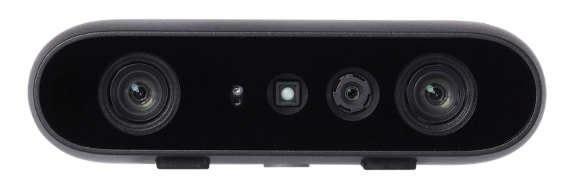
\includegraphics[width=0.7\textwidth]{gemini2.png}
    \caption{奥比中光RGB-D视觉传感器Gemini 2正视实物图。}
    \label{fig:aobi_robot}
  \end{figure}
\textbf{识别准确率。}
为了评估系统的识别准确性,本文使用商业级奥比中光RGB-D相机(图~\ref{fig:aobi_robot})构建了自采数据集,并基于此评估了本文的方法。%本实验共召集\textcolor{red}{xx}名志愿者
共采集了12类数据,每类包含25个样本(图~\ref{fig:aobi_sample})。%参与数据采集的志愿者共计。%均来自xxx,涵盖不同性别、年龄及手势习惯,以确保数据的多样性与代表性。
采集过程遵循\cite{wan2016chalearn}的设置,采集分辨率为$320\times240$,平均帧数32,每帧同时包含RGB图像和Depth图像。
结果显示,所提出的识别算法,在RGB-D模态的识别准确率达到了99.27\%,验证了所提出方法在实际应用场景中的高效性与可靠性。

\begin{figure}
    \centering
    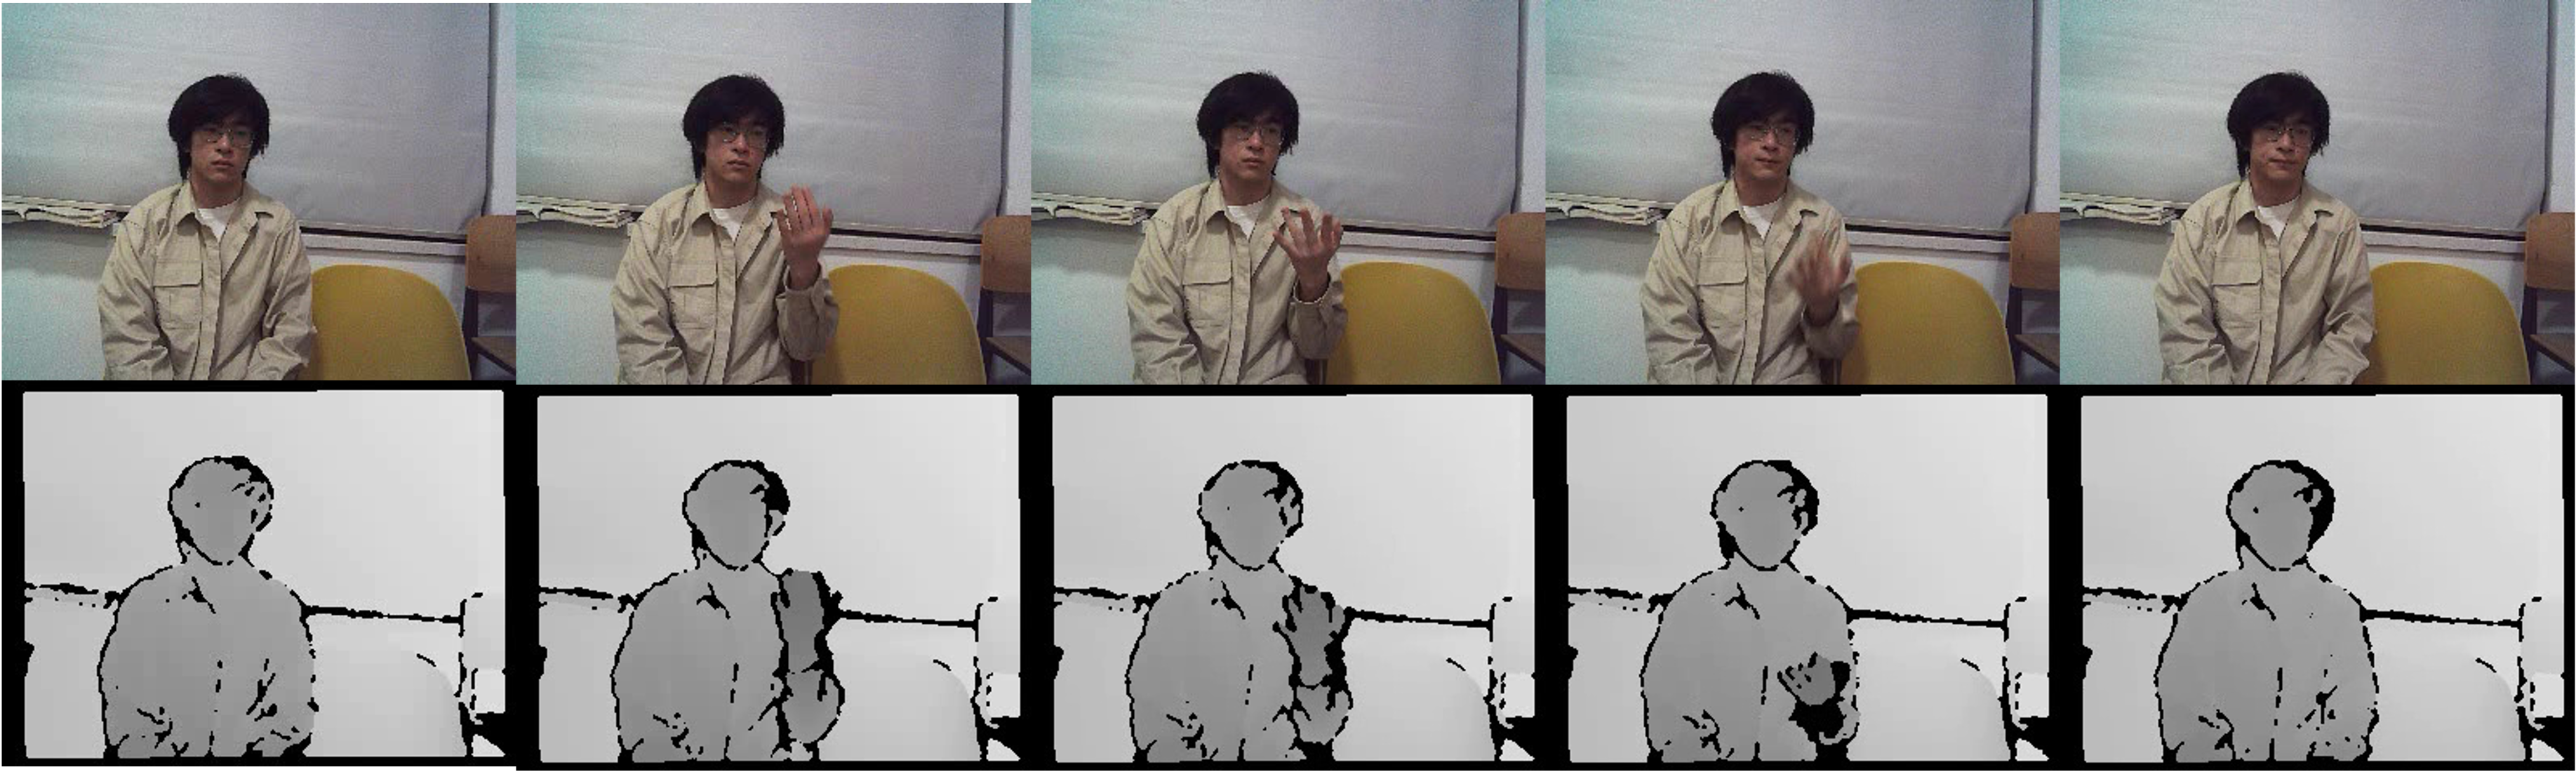
\includegraphics[width=0.8\linewidth]{aobi_sample.png}
    % \caption*{}
    \caption{商业RGB-D相机自采数据集样本示例。}
    \label{fig:aobi_sample}
  \end{figure}

% 目前已采集x类xx数据(数据格式)
% 测试结果


\textbf{识别推理速度。}
本文在单张RTX2080显卡上对手语识别模块进行了推理速度测试,对同一样本进行了五次测试。如图\ref{fig:time}所示,平均推理时间为83.9ms,快于基线方法\cite{范桂双2020基于S3D}所公布的96ms。这表明本文的算法模块具有高效的推理能力,能够满足实时交互需求。

\begin{figure}
  \centering
  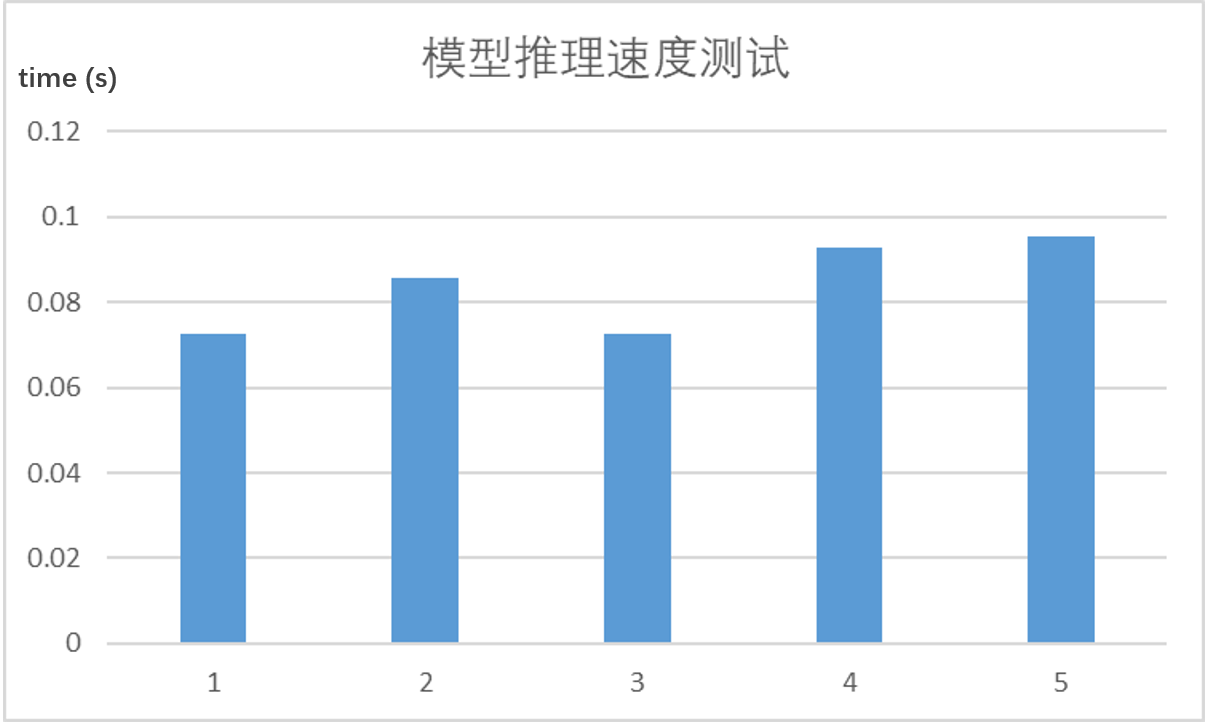
\includegraphics[width=0.65\linewidth]{time.png}
  % \caption*{}
  \caption{手语识别模块推理时间(单位:ms)。}
  \label{fig:time}
\end{figure}


\textbf{用户感知研究。}
本文进行了用户研究以评估系统生成的手部动作质量。本文招募了20名参与者评估10对9秒的结果。每个生成结果从两个个方面进行评估:(i) \textit{自然度}:生成的动作与人类手势相比的真实性和自然度;(ii) \textit{匹配度}:生成的动作对给定文本描述的反映准确度。在每次评估环节中,参与者观看不同模型生成的视频片段,并针对每个方面选择表现最佳的方法。
如表~\ref{tab:perceptual_study}所示,本文的方法具有优胜的用户偏好。

\begin{table}[t]
    \centering
    \caption{手部动作生成结果的用户偏好胜率(\%)。结果表明本文生成的结果被认为更加真实和可控,在自然度和匹配度方面分别优于之前的工作~\cite{chen2024syntalker}4.65\%和1.87\%。}
    \small
    \label{tab:perceptual_study}
    \begin{tabular}{c cc}
    \toprule
    方法 & 自然度 & 匹配度 \\
    \midrule
    基线1~\cite{yang2024freetalker} & 20.93  & 19.38 \\
    基线2~\cite{chen2024syntalker} & 37.21  & 39.38 \\
    本文方法 & 41.86  & 41.25 \\
    \bottomrule
    \end{tabular}
\end{table}

% \subsection{用户评估实验设计}
% \textcolor{red}{
% 为全面评估系统的实际应用效果,本文设计了系统化的用户评估实验。实验招募了10名手语初学者作为测试者,实验内容包括基础手语词汇学习(10个常用手语词汇)和简单手语句子练习(5个日常用语)两个部分。
% 实验采用多维度评估指标,包括:学习效率(完成学习任务所需时间)、识别准确率(系统识别用户手语动作的准确程度)、用户满意度(基于问卷的主观评分,1-5分)以及系统可用性(基于SUS量表的评估)。实验结果显示,参与者平均用时45分钟完成全部学习任务,系统识别准确率达到92\%,用户满意度评分平均为4.3分,SUS评分为85分,表明系统具有良好的学习辅助效果和用户体验。}
    
    

    
\section{本章小结}
本章详细介绍了交互式手语学习助手系统的设计与实现。系统基于本文提出的MDSI手势识别算法和CoordSpeaker协同手势生成算法,实现了实时手语动作评估、标准手语动作生成功能。通过模块化设计和高效的系统架构,成功构建了一个具有实时性、准确性和良好交互体验的手语学习辅助系统。%系统测试与用户评估结果表明,该系统能够有效辅助手语学习,具有良好的实用价值。
未来工作将进一步优化系统性能,扩展学习内容库,提升系统的实用性和适用范围。

% % % 应用
% \section{基于RGB-D手势识别的机器人导航控制系统}
% \label{sec:robot}
% 本文拟基于所提出的 MDSI 动态手势识别算法构建一个机器人手势导航控制交互系统,并部署于奥比中光机器人平台。旨在帮助用户更好地实现机器人控制操作,同时提升手势控制过程中的人机交互体验。

% \subsection{奥比中光机器人平台}
% % 简介
% 奥比中光机器人平台(图\ref{fig:aobi_robot})是一种基于RGB-D深度视觉传感器的智能交互系统,支持实时环境感知与多模态交互能力。该平台配备高精度深度摄像头和集成式开发工具包,可捕捉手部动作的空间轨迹,进而实现多种复杂任务的导航控制与交互。

% 该平台采用主动双目结构光3D视觉传感器Gemini 2,其测试结果表明,其性能完全满足技术需求,具体包括以下参数:
% \begin{itemize}
%   \item \textbf{深度图像分辨率及帧率}:640x360@30fps,确保高质量的深度感知能力;
%   \item \textbf{测量范围}:300mm-700mm,适应多种交互距离;
%   \item \textbf{视场角}:D-FoV=99.5°@500mm,提供广阔的环境感知范围;
%   \item \textbf{测量精度}:在25\%中心区域达到0.35mm@500mm的精度,确保手势追踪的细腻与精准;
%   \item \textbf{功耗}:1.663W,支持长时间的低功耗运行;
%   \item \textbf{接口}:USB 3.0,支持高速数据传输与设备兼容性。
% \end{itemize}

% 此外,该平台的主要功能特点包括:1)\textbf{高精度深度感知}:通过RGB-D相机实现毫米级手势追踪和三维空间定位;2)\textbf{实时处理性能}:基于嵌入式硬件和深度学习推理加速,支持快速的手势识别与响应;
% 3)\textbf{灵活的扩展性}:支持多种机器人设备接口协议,可广泛应用于导航、巡逻、助理服务等场景。
% Gemini 2的优秀性能和平台的多模态交互能力,为机器人导航控制提供了高效、可靠的技术支持。


% \begin{figure}[htbp]
%   \centering
%   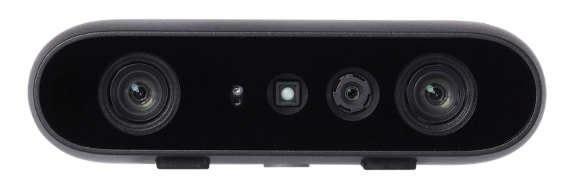
\includegraphics[width=0.7\textwidth]{gemini2.png}
%   \caption{奥比中光产品主动双目结构光3D视觉传感器Gemini 2正视实物图。}
%   \label{fig:aobi_robot}
% \end{figure}

% \begin{figure}[htbp]
%   \centering
%   \begin{subfigure}{0.7\textwidth}
%     \centering
%     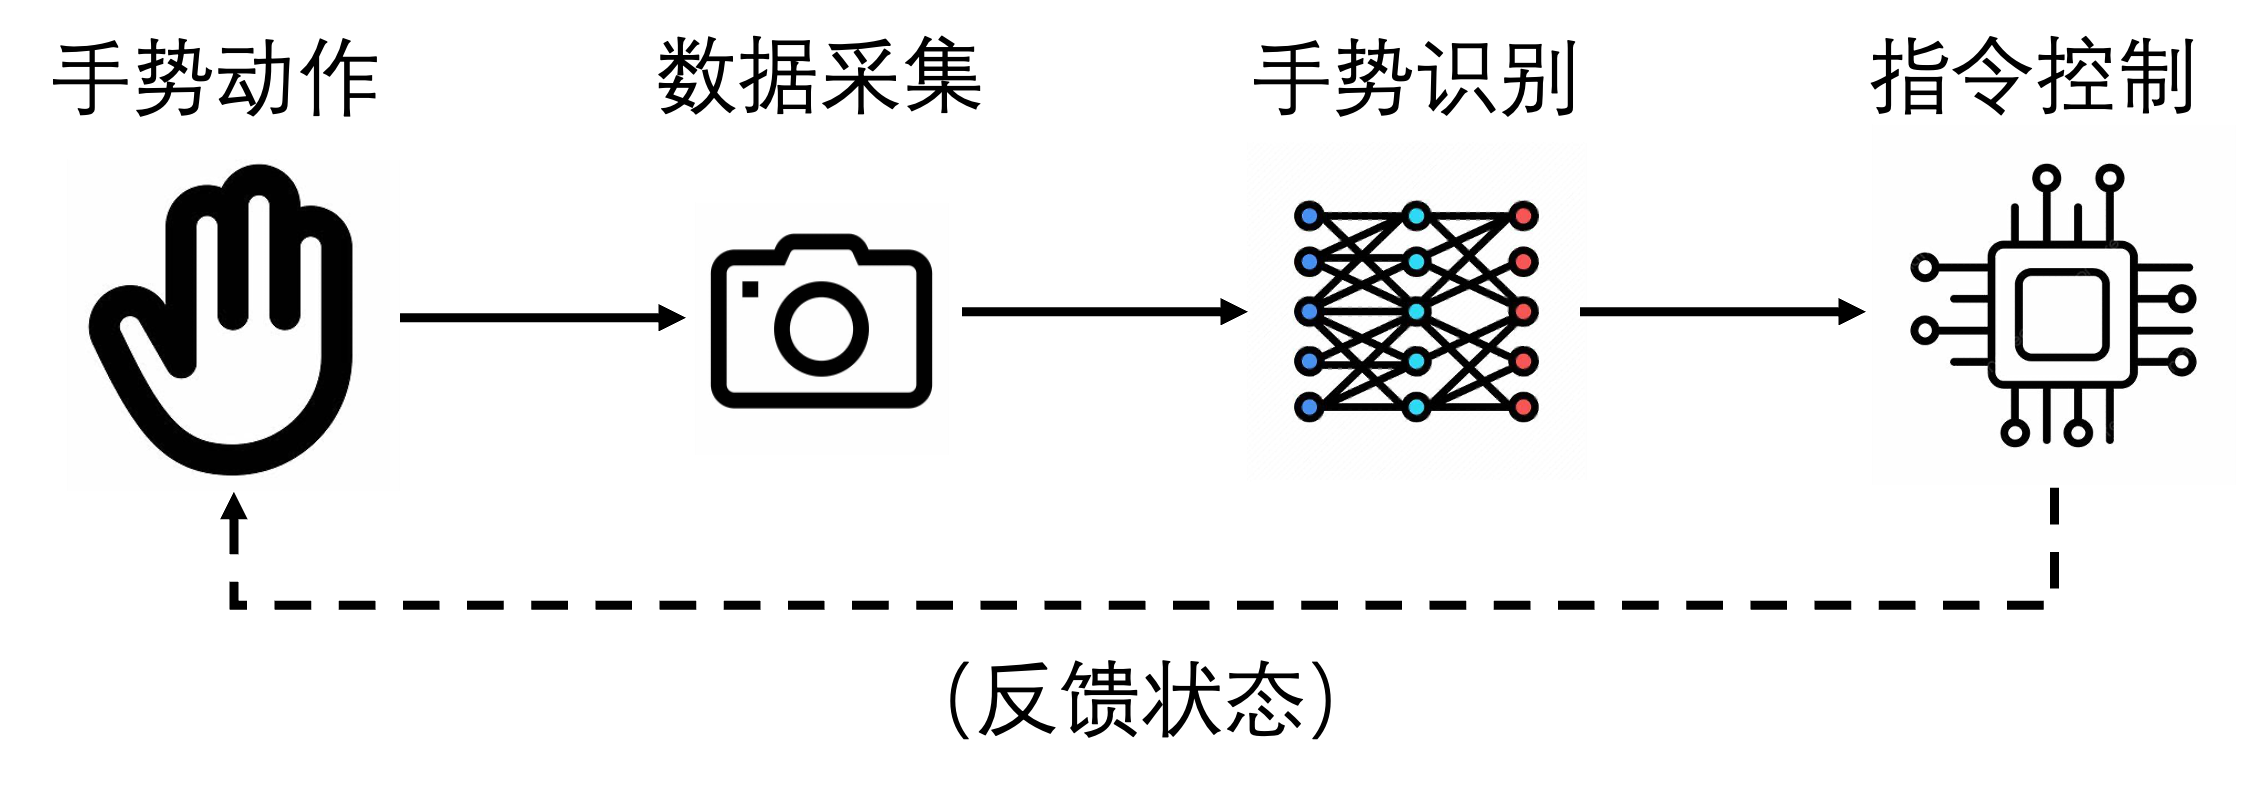
\includegraphics[width=\textwidth]{arch.png}%{system.png}
%     \caption{}
%     \label{fig:nav_control_ui}
%   \end{subfigure}
%   \hfill
%   \begin{subfigure}{0.8\textwidth}
%     \centering
%     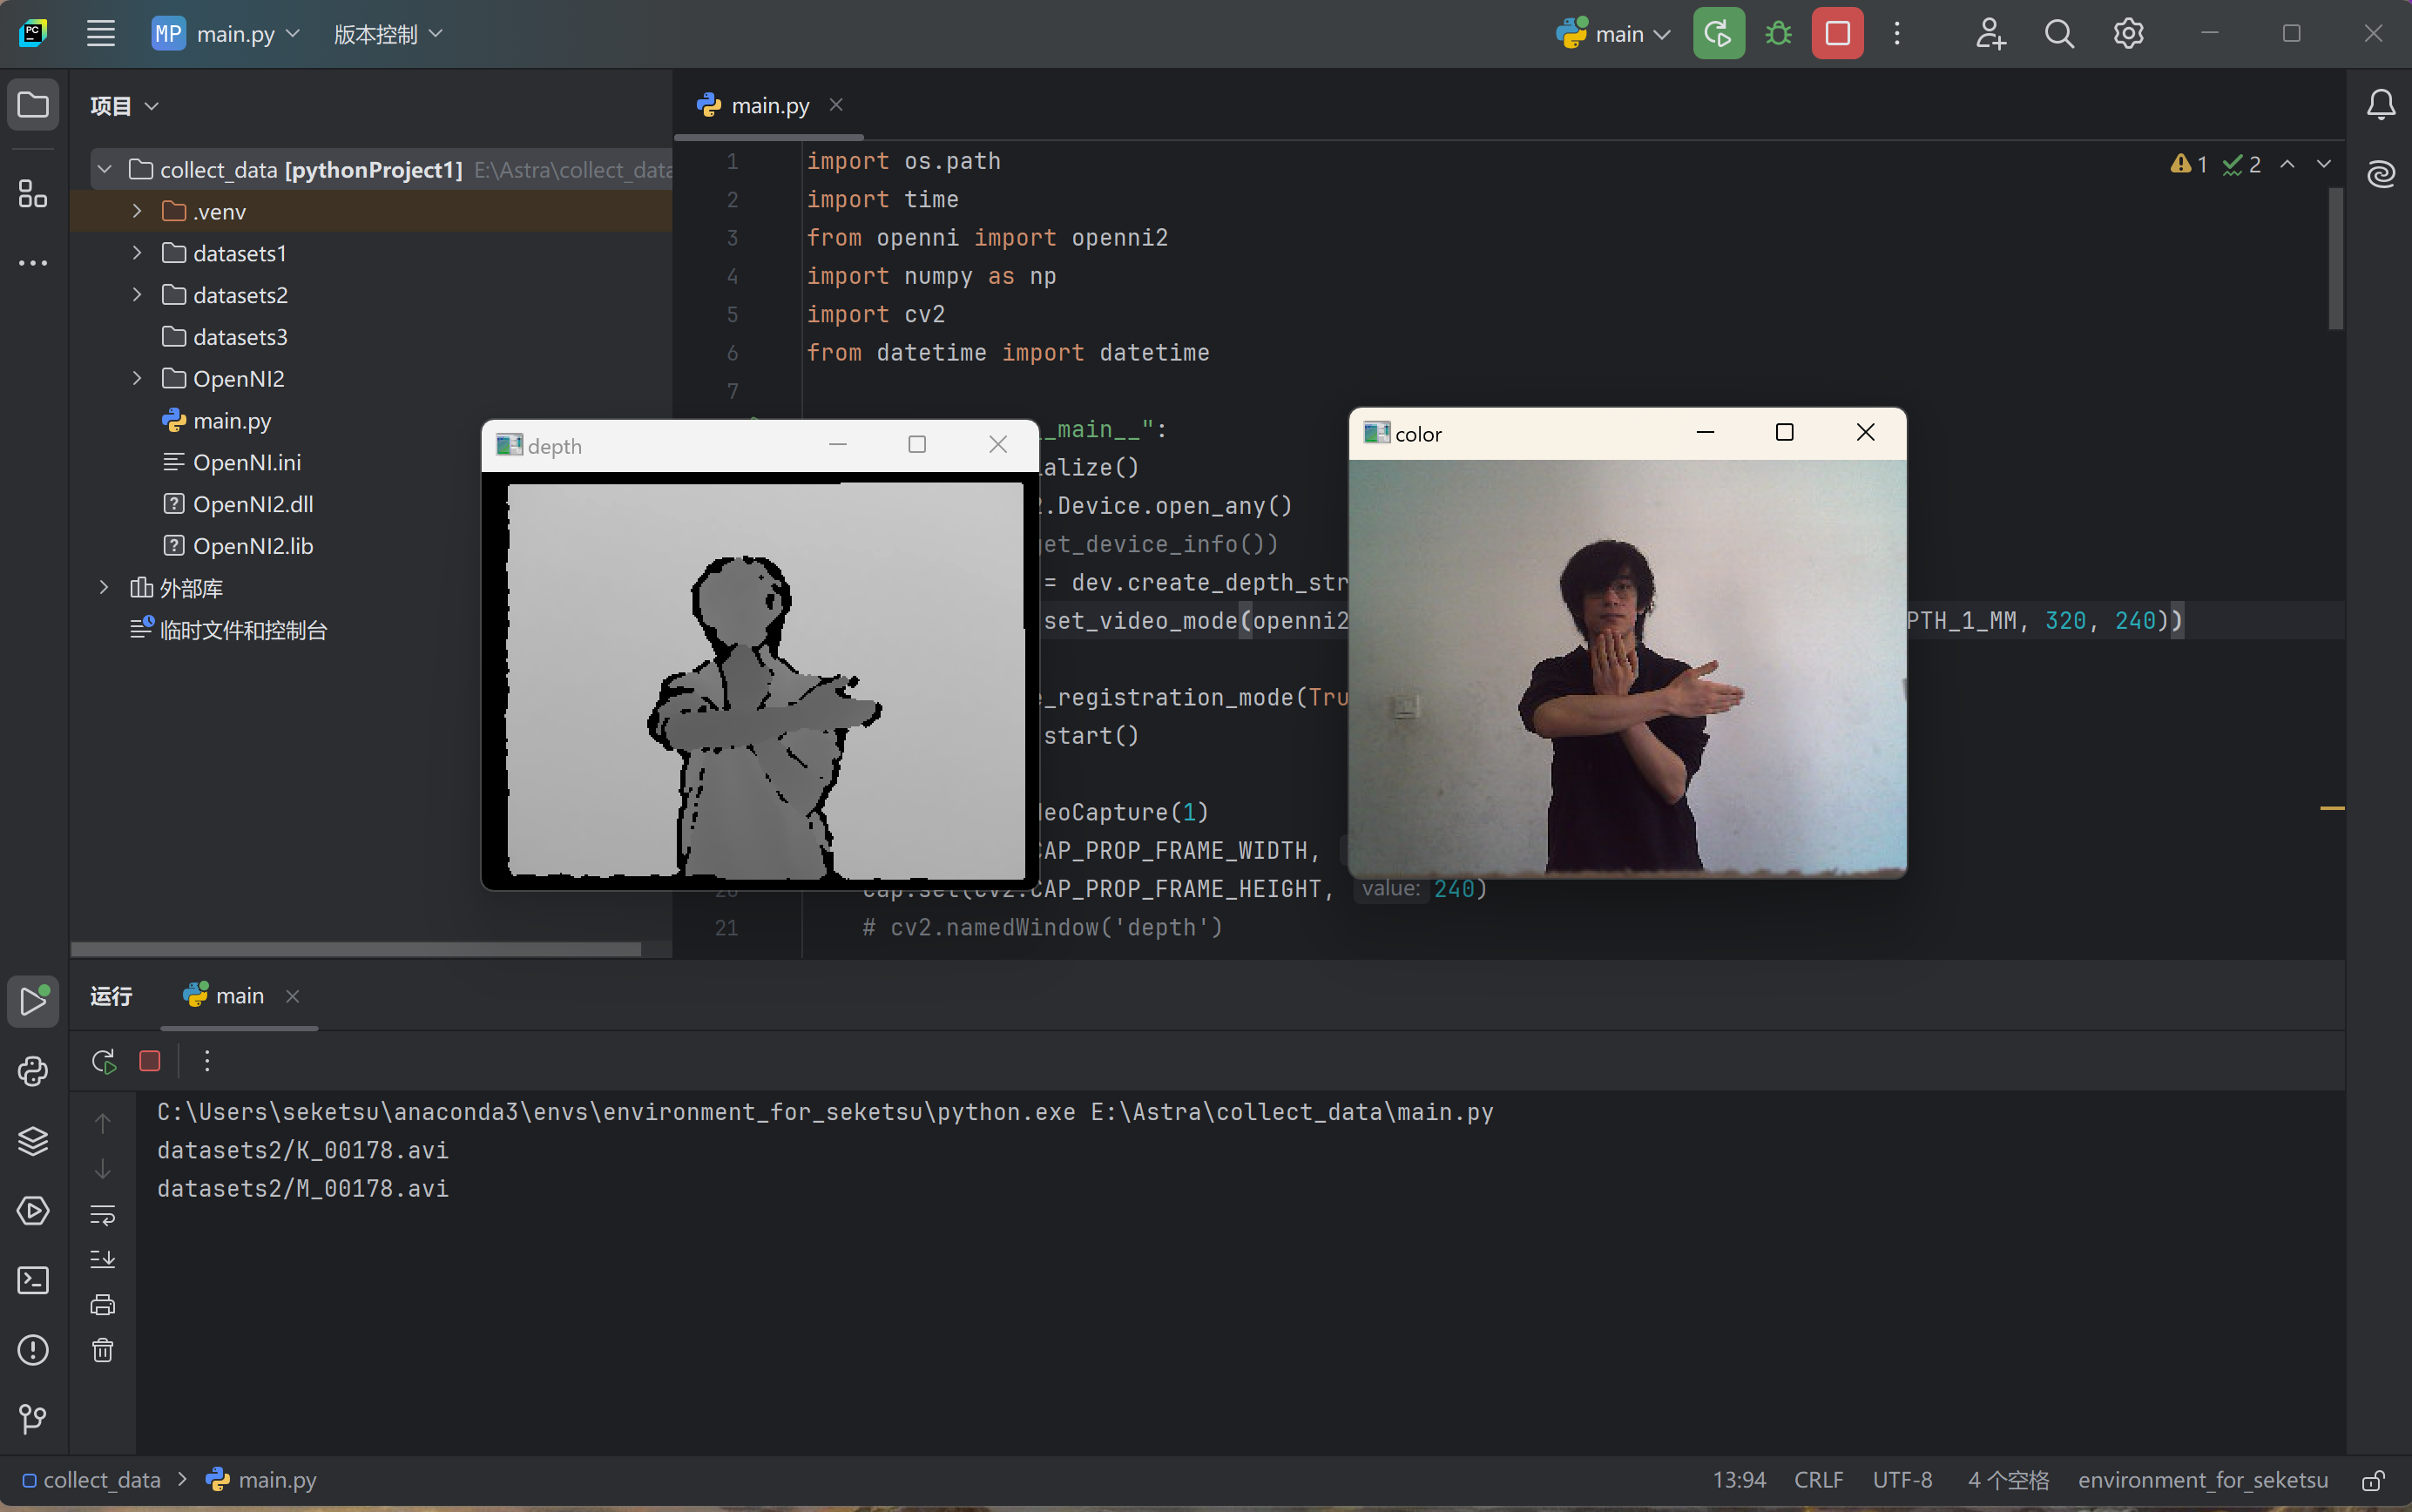
\includegraphics[width=\textwidth]{collect-min.png}%{prototype.png}
%     \caption{}
%     \label{fig:data_collection_ui}
%   \end{subfigure}
%   \caption{手势导航控制系统架构。(a)手势导航控制应用原型,(b)手势数据采集工具界面。}
% \end{figure}

% \subsection{手势导航控制应用}
% % 原型图
% 为了实现基于MDSI动态手势识别算法的机器人导航控制功能,本文设计了一个完整的手势导航控制系统(图\ref{fig:nav_control_ui}),涵盖手势数据采集、手势识别与指令生成以及机器人控制三个关键阶段。  
% \begin{enumerate}
%   \item \textbf{手势数据采集}:本文首先开发了一款手势视频采集工具,用于录制和存储用户执行的各种手势动作。该工具具有直观的操作界面,支持实时预览和手势标签标注功能。用户在指定区域内完成手势动作,系统将采集的视频数据存储为RGB-D格式,%并附带时间戳和空间坐标信息,
%   便于后续训练与分析。图\ref{fig:data_collection_ui}展示了手势数据采集工具的界面截图,其中包括实时相机预览窗口、手势类别选择按钮,以及数据保存路径设置模块。  
%  \item \textbf{手势识别与指令生成}:通过MDSI算法对采集的RGB-D手势数据进行实时处理,系统可精准解析用户意图并生成对应的导航指令(如"向前移动"、"左转")。该模块采用高效的多模态融合策略,确保在复杂背景下的高识别率。  
%   \item \textbf{机器人控制}:解析后的手势指令通过通信接口传递给机器人平台,用于导航控制。机器人在执行过程中实时反馈状态信息(如位置、速度),以便用户随时调整指令。  
% \end{enumerate}



% 为了展示基于MDSI动态手势识别算法的实际应用效果,本文设计了一个机器人导航控制应用原型。用户通过手势控制机器人完成基本的导航任务,例如向前、向后、左转、右转、停止等。原型设计如下:

% \begin{enumerate}
%   \item 系统架构:
%   \begin{itemize}
%     \item RGB-D相机捕获用户手势信息,通过MDSI算法实时识别并解析手势指令。
%     \item 系统将解析后的手势指令传递给机器人,通过平台接口控制其移动。
%   \end{itemize}
%   \item 交互逻辑:
%   \begin{itemize}
%     \item 用户在指定区域内执行手势动作,系统显示实时反馈以确认手势识别结果。
%     \item 用户可随时更改手势指令,以调整机器人的行进路径。
%   \end{itemize}
%   \item 界面原型:包含实时摄像头画面、手势识别反馈、机器人位置状态等模块。
%   \begin{itemize}
%     \item 实时摄像头画面:展示用户手势动作。
%     \item 识别结果与指令反馈:在中央显示当前识别到的手势及对应的指令(如"向前移动")。
%     \item 机器人状态面板:右侧显示机器人位置、速度及电池状态信息。
%   \end{itemize}
% \end{enumerate}
% 以下为原型设计图:

% 以下为数据采集界面截图:




% \section{\textcolor{red}{增强现实环境下的实时手语翻译系统设计}}

% 本文拟构建一个增强现实(AR)环境下的实时手语翻译系统,基于所提出的多流解耦手势识别算法搭建实时手语翻译应用,并部署于可穿戴AR眼镜。旨在帮助手语者更好地表达自己并维护自己的权益,同时提升手语沟通过程中的人机交互体验。
% \subsection{实时手语翻译算法管线}
% 实时手语翻译算法管线包括手语识别(SLR)和手语翻译(SLT)两个阶段\cite{chen2022two}。图\ref{fig:SLRSLT}进一步阐述了SLR与SLT的作用:与手势识别相似的,手语识别 (SLR) 旨在将输入的手语视频转录为注释序列;而手语翻译 (SLT) 直接预测给定手语视频的文本,大多数方法通过使用视觉编码器作为标记器来提取视觉特征并将其转发到翻译网络以生成口语文本,从而将该任务表述为神经机器翻译(NMT)问题\cite{chen2022two}。
% 本文使用所提出的多流解耦注意力模型作为SLR网络,并计划使用具有出色手语翻译性能的mBART\cite{liu2020multilingual}作为本文的SLT网络。
% 为了获得满意的结果,本文使用在手势识别任务上预训练好的SLR网络,并基于手语翻译数据集CSL-Daily联合微调SLR与SLT。
% 连续手势的分割是使用基于先验知识(手的放下与抬起)的手部检测进行的。
% 图\ref{fig:SLRpipe}展示了本文的实时手语翻译算法管线。
% \begin{figure}
%   \centering
%   \subcaptionbox{SLR与SLT的阐释\cite{chen2022two}\label{fig:SLRSLT}}
%     {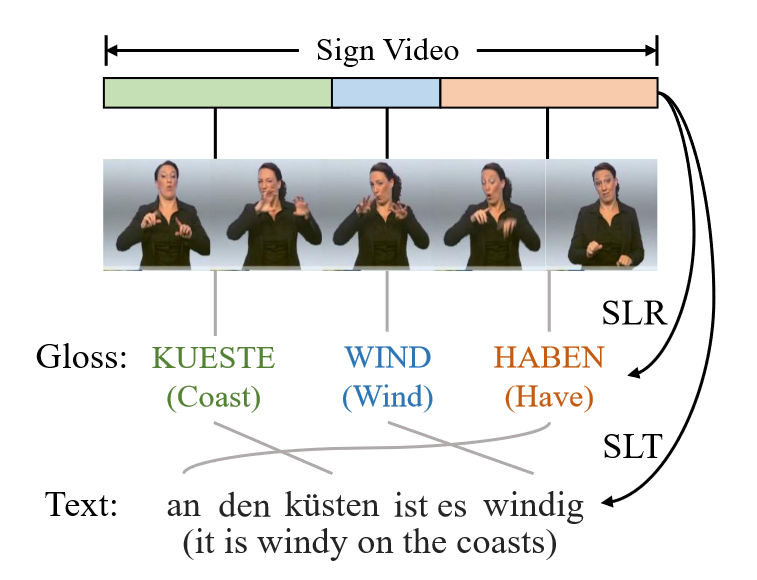
\includegraphics[width=0.5\linewidth]{SLRSLT.png}}
%   \subcaptionbox{实时手语翻译算法管线\label{fig:SLRpipe}}
%     {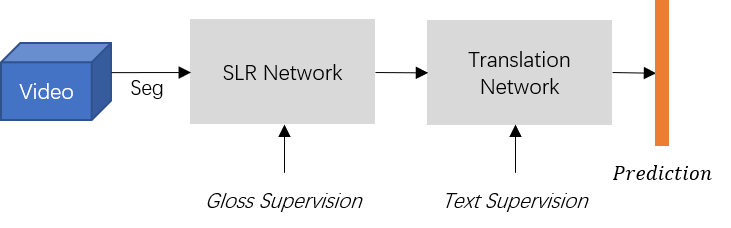
\includegraphics[width=0.8\linewidth]{SLRpipe.png}}
%   \caption{AR实时手语翻译系统原型}
%   \label{fig:SLRpipeline}
% \end{figure}

% \subsection{AR实时手语翻译应用原型设计}
% \begin{figure}
%   \centering
%   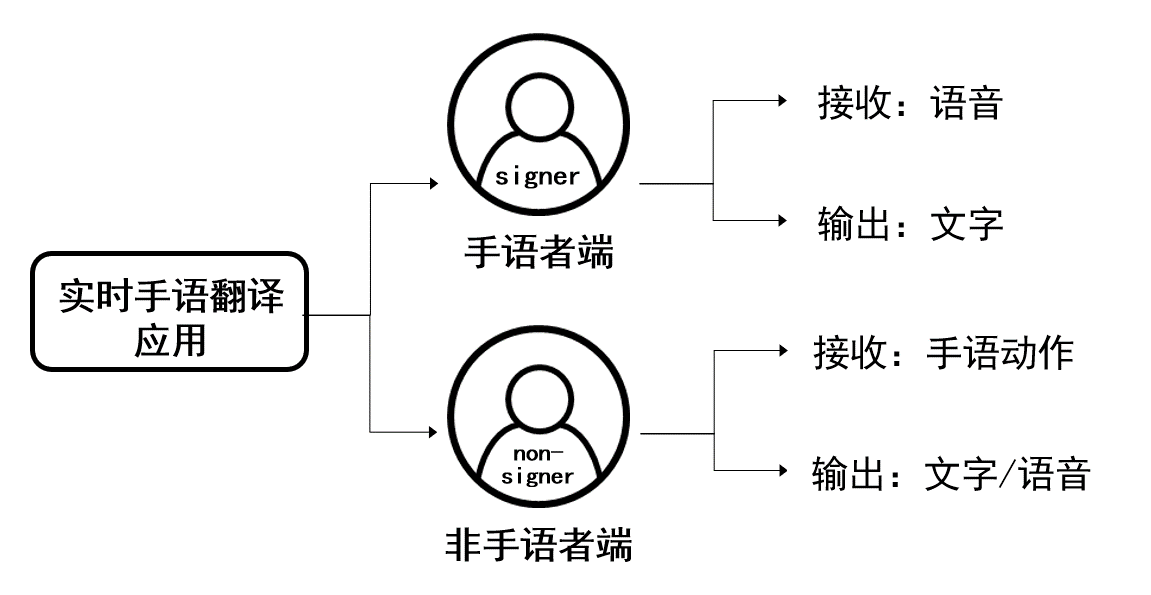
\includegraphics[width=0.8\linewidth]{system.png}
%   % \caption*{}
%   \caption{增强现实(AR)环境下的实时手语翻译系统功能设计}
%   \label{fig:system}
% \end{figure}
% 图\ref{fig:system}展示了实时手语翻译系统的基本功能设计。系统包括"手语者端"与"非手语者端":"手语者端"通过麦克风与智能语音识别API捕捉所听到的声音信号,并进行实时翻译,转换为文字显示在AR眼镜屏幕上;"非手语者端"则通过摄像头以及本文的手势识别技术,捕获手语者做出的手势动作并进行实时翻译,转换为文字显示在AR眼镜屏幕上。图\ref{fig:prototype}展示了一个简单的手语翻译系统使用场景,手语者正做出代表"Love"的手势动作,翻译所得的语义展示在AR眼镜屏幕上。

% % \begin{figure}
% %   \centering
% %   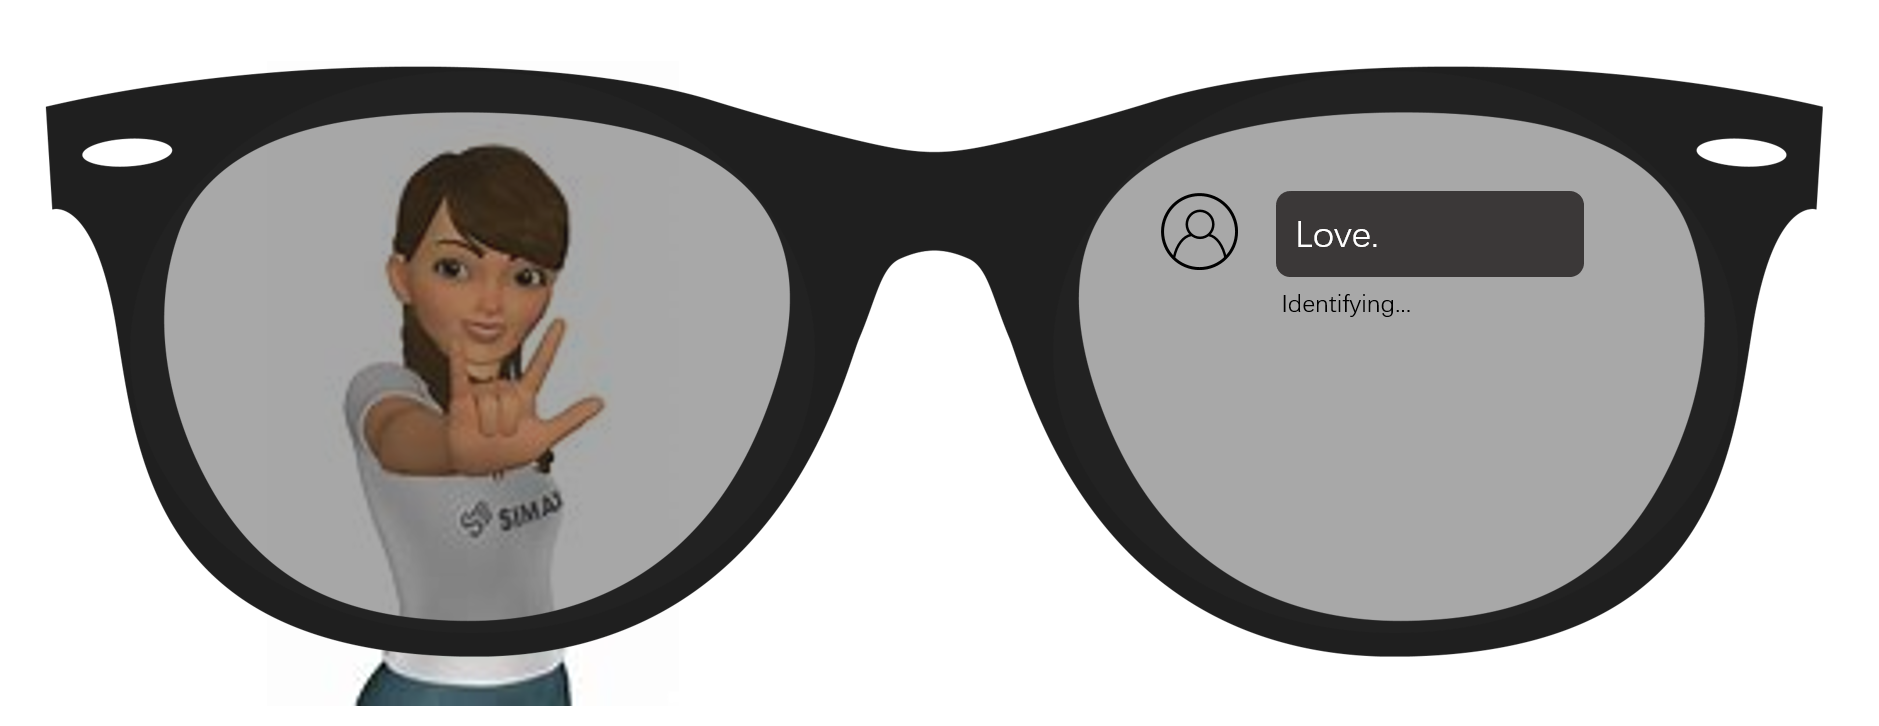
\includegraphics[width=0.9\linewidth]{prototype.png}
% %   \caption*{手语者正做出代表"Love"的手势动作,翻译所得的语义展示在AR眼镜屏幕上}
% %   \caption{一个简单的手语翻译系统使用场景}
% %   \label{fig:prototype}
% % \end{figure}

% \begin{figure}
%   \centering
%   \subcaptionbox{原型设计\label{fig:prototypea}}
%     {
\includegraphics[width=0.65\linewidth]{prototypea.png}}
%   \subcaptionbox{使用场景示例:手语者正做出代表"Love"的手势动作,翻译所得的语义将展示在AR眼镜屏幕上\label{fig:prototypeb}}
%     {\includegraphics[width=0.65\linewidth]{prototypeb.png}}
%   \caption{AR实时手语翻译系统原型}
%   \label{fig:prototype}
% \end{figure}  % 交互式手语学习助手设计与实现
% !TeX root = ../thuthesis-example.tex

\chapter{总结与展望}
\label{sec:summary}

\section{工作总结}
本文针对手语辅助教学中存在的动作评估困难、标准教学资源匮乏等问题,基于深度学习技术开展了手势识别与生成算法研究,并设计实现了一个交互式手语学习助手系统。主要研究工作及其创新成果如下:

(1)在手势识别方面,本文提出了一种多模态的多策略解耦和语义集成网络(MDSI)。该方法通过“姿势-运动”和“时空-通道”特征解耦,有效缓解了RGB-D手势识别中的信息冗余问题。同时引入语义滤波器和标签平滑机制,增强了语义理解能力,实现了对视觉相似手势的精确区分。在IsoGD和THU-READ两个主流基准测试中,MDSI实现了最先进的识别准确率,相比现有最优方法分别提升了2.48\%和1.27\%。此外,通过可插拔设计,模型在保持性能的同时,参数量仅占主干网络的6.84\%。

(2)在手势生成方面,本文设计了一种基于描述驱动的协同手势生成框架(CoordSpeaker)。该框架首次引入手势描述生成模块,创新性地解决了手势数据缺乏描述性文本标注的问题。通过统一的运动表示方法和可控的潜在扩散模型,实现了语义和节奏的协同精确控制。大量定量与定性实验结果表明,该方法能够有效生成高质量的(Jerk $0.529\rightarrow$)、语音同步(BC $0.180\uparrow$)、语义相关(MM-Dist: $6.814$)的协同手势运动,优于现有方法。此外,通过优化的潜在扩散过程,模型的平均推理时间(AITS)仅为0.842秒,较现有方法提升了6倍以上,显著增强了系统的实用性。
% 定量结果也表明,该方法在多个评估指标上均优于现有方法:语义相关性指标MM-Dist降低至6.814,动作自然度指标FID降低了25.6\%,同时保持了良好的语音同步性(BC: 1.327)和动作多样性(L1Div: 10.861)。特别地,通过高效的分层去噪架构和

(3)基于上述算法创新,本文设计并实现了一个交互式手语学习助手系统。该系统采用模块化架构设计,集成了实时手语识别、标准动作生成和交互反馈等功能模块。系统支持手语学习、练习评估和自由练习三种主要交互模式,并提供了清晰的分区布局与友好的交互界面引导。基于商业级RGB-D相机开展的实验证明,系统能够实现高效、可靠的识别评估(12类数据识别准确率\textgreater 99\%,推理时间\textless 0.1s),并能生成高质量的、用户满意的手部动作(自然度偏好高于同类方法 4.0\%)。
系统的实现验证了本文提出算法的实用价值,为解决手语教学资源匮乏的问题提供了新的技术途径。

本文的主要创新点体现在算法研究、应用实践两个层面。首先,在算法层面,针对手势识别中的“信息冗余”与“信息缺失”挑战提出了“多策略解耦与语义集成手势识别(MDSI)”网络,提升了手势识别的效率与准确性;针对手势生成中的描述注释缺失和多模态协同控制困难的挑战,设计了“基于描述驱动的协同手势生成框架(CoordSpeaker)”,实现了高效与高质量的协同手势生成。其次,在应用层面,本文首次实现了“基于深度学习的交互式手语学习系统”,针对手语教学中的实时评估和资源匮乏挑战,提出了有效的算法解决方案,为听障人士的手语学习提供了新途径。

\section{研究展望}
本文虽在手势识别与生成领域取得了一些进展,但仍有多个方向值得进一步探索。后续研究可从以下几个维度深入:

(1)手势识别算法方面,目前采用的多分支特征融合策略仍较为简单,主要依赖于分数融合方法。未来可以探索更复杂和精细的多模态联合建模机制,如注意力引导的特征交互、跨模态对比学习等方法,以充分挖掘不同模态信息之间的互补性,进一步提升识别系统的性能和鲁棒性;
此外,针对手语识别引入更丰富的模态特征(如语音、面部表情等)是一个具有前景的研究方向。这些额外的模态信息有望为手语理解提供更丰富的语义线索,但同时也需要构建包含多模态标注的大规模数据集作为支撑;
最后,本文证明了 MDSI 灵活、可插拔的特性使其能够无缝集成到各种架构中,并能轻松适应其他领域,例如动作识别和手语识别。由于集成所需的调整很少,进一步探索 MDSI 与各种主干的集成仍然是一个有价值的方向,例如与新兴的多模态大模型结合可能带来增强的效果,并且轻微的定制可以产生有益的结果。

(2)手势生成算法方面,虽然本文提出的手势描述生成模块在一定程度上缓解了手势生成中的语义控制问题,但模型对精细手部动作(如手指细节)的描述和生成能力仍有待提升。未来可以探索基于人体骨架的分层次生成策略,将全身动作、手臂运动和手指姿态分别建模,并设计合理的协同机制,以提升生成结果的精确度和自然度。同时,引入更丰富的上下文信息和情感特征,有望进一步增强生成手势的表现力。

(3)手语学习系统方面,当前系统仅支持单个词汇级的识别和生成,在处理复杂手语句子方面仍有较大局限性。未来研究可以围绕手语语法规则建模、上下文语义理解等关键技术展开深入探索,结合自然语言建模技术,逐步实现对连续手语句子的准确识别和流畅生成;此外,系统的交互体验和个性化学习支持也有待进一步优化。当前系统交互以视觉为主,未来可以引入语音、触觉等多种交互方式,并探索基于增强现实的沉浸式学习环境;最后,系统的动态扩展能力可进一步加强,虽然目前手势生成模块支持自由灵活的词汇生成、但手势识别模块目前仅支持预定义的词汇评估。未来可以探索基于主动学习的在线增量学习机制,使系统能够从用户交互中持续学习新的手语词汇和动作,动态扩展识别和生成能力。
% 如引入多模态的交互、自适应学习策略、更丰富的学习模式等,为用户提供更加智能和沉浸式的学习环境。
  % 总结与展望


% 其他部分
\backmatter

% 参考文献
\bibliography{ref/refs}  % 参考文献使用 BibTeX 编译
% \printbibliography       % 参考文献使用 BibLaTeX 编译

% 附录
% 本科生需要将附录放到声明之后,个人简历之前
\appendix
% % !TeX root = ../FFY_graduate.tex

\begin{survey}
\label{cha:survey}

\title{Title of the Survey}
\maketitle


\tableofcontents


本科生的外文资料调研阅读报告。


\section{Figures and Tables}

\subsection{Figures}

An example figure in appendix (Figure~\ref{fig:appendix-survey-figure}).

\begin{figure}
  \centering
  \includegraphics[width=0.6\linewidth]{example-image-a.pdf}
  \caption{Example figure in appendix}
  \label{fig:appendix-survey-figure}
\end{figure}


\subsection{Tables}

An example table in appendix (Table~\ref{tab:appendix-survey-table}).

\begin{table}
  \centering
  \caption{Example table in appendix}
  \begin{tabular}{ll}
    \toprule
    File name       & Description                                         \\
    \midrule
    thuthesis.dtx   & The source file including documentaion and comments \\
    thuthesis.cls   & The template file                                   \\
    thuthesis-*.bst & BibTeX styles                                       \\
    thuthesis-*.bbx & BibLaTeX styles for bibliographies                  \\
    thuthesis-*.cbx & BibLaTeX styles for citations                       \\
    \bottomrule
  \end{tabular}
  \label{tab:appendix-survey-table}
\end{table}


\section{Equations}

An example equation in appendix (Equation~\eqref{eq:appendix-survey-equation}).
\begin{equation}
  \frac{1}{2 \uppi \symup{i}} \int_\gamma f = \sum_{k=1}^m n(\gamma; a_k) \mathscr{R}(f; a_k)
  \label{eq:appendix-survey-equation}
\end{equation}


\section{Citations}

Example citations in appendix.
\cite{abrahams99tex}
\cite{salomon1995advanced}
\cite{abrahams99tex,salomon1995advanced}


\bibliographystyle{unsrtnat}
\bibliography{ref/appendix}

\end{survey}
       % 本科生:外文资料的调研阅读报告
% % !TeX root = ../FFY_graduate.tex

\begin{translation}
\label{cha:translation}

\title{书面翻译题目}
\maketitle

\tableofcontents


本科生的外文资料书面翻译。


\section{图表示例}

\subsection{图}

附录中的图片示例(图~\ref{fig:appendix-translation-figure})。

\begin{figure}
  \centering
  \includegraphics[width=0.6\linewidth]{example-image-a.pdf}
  \caption{附录中的图片示例}
  \label{fig:appendix-translation-figure}
\end{figure}


\subsection{表格}

附录中的表格示例(表~\ref{tab:appendix-translation-table})。

\begin{table}
  \centering
  \caption{附录中的表格示例}
  \begin{tabular}{ll}
    \toprule
    文件名          & 描述                         \\
    \midrule
    thuthesis.dtx   & 模板的源文件,包括文档和注释 \\
    thuthesis.cls   & 模板文件                     \\
    thuthesis-*.bst & BibTeX 参考文献表样式文件    \\
    thuthesis-*.bbx & BibLaTeX 参考文献表样式文件  \\
    thuthesis-*.cbx & BibLaTeX 引用样式文件        \\
    \bottomrule
  \end{tabular}
  \label{tab:appendix-translation-table}
\end{table}


\section{数学公式}

附录中的数学公式示例(公式\eqref{eq:appendix-translation-equation})。
\begin{equation}
  \frac{1}{2 \uppi \symup{i}} \int_\gamma f = \sum_{k=1}^m n(\gamma; a_k) \mathscr{R}(f; a_k)
  \label{eq:appendix-translation-equation}
\end{equation}


\section{文献引用}

文献引用示例\cite{abrahams99tex}。


\appendix

\section{附录}

附录的内容。


% 书面翻译的参考文献
\bibliographystyle{unsrtnat}
\bibliography{ref/appendix}

% 书面翻译对应的原文索引
\begin{translation-index}
  \nocite{salomon1995advanced}
  \bibliographystyle{unsrtnat}
  \bibliography{ref/appendix}
\end{translation-index}

\end{translation}
  % 本科生:外文资料的书面翻译
% !TeX root = ../thuthesis-example.tex

\chapter{可视化结果}
\label{sec:appendix_vis}
% 在补充材料中,我们提供了更多实施细节(第 6 节)、额外的实验结果(第 7 节)、更多可视化结果(第 8 节)、局限性讨论(第 9 节)以及用户研究伦理考虑(第 10 节)。
本章提供了更多手势生成的可视化结果。

\textbf{协同生成结果。}
图~\ref{fig:vis_supply}展示了更多的协同手势生成结果,使用相同的音频和不同的文本标题控制生成。
这些结果进一步证实了本文提出的方法在联合语音字幕控制下生成协同的语音自发手势和字幕驱动的非自发运动的有效性。

% 更多手势字幕结果
\textbf{手势描述结果。}
图~\ref{fig:vis_caption_supply}展示了更多的手势描述结果,彩色框突出显示了手势和文本字幕之间的精确映射,进一步证明了本文的方法在准确地将手势映射到文本方面的有效性。
正如彩色框显示,该模型在描述复杂、连续的动作时成功捕捉了细粒度的手部动作和粗粒度的全身动作。

\begin{figure*}[t]
  \centering
  \includegraphics[width=\linewidth]{visualization_supply.png}
  \caption{协同手势生成结果。}
  \label{fig:vis_supply}
\end{figure*}

\begin{figure*}[t]
  \centering
  \includegraphics[width=\linewidth]{visualization_caption_supply.png}
  \caption{手势描述结果。}%彩色框突出显示了手势和文本字幕之间的精确映射。}
  \label{fig:vis_caption_supply}
\end{figure*}

% 附录是与论文内容密切相关、但编入正文又影响整篇论文编排的条理和逻辑性的资料,例如某些重要的数据表格、计算程序、统计表等,是论文主体的补充内容,可根据需要设置。

% 附录中的图、表、数学表达式、参考文献等另行编序号,与正文分开,一律用阿拉伯数字编码,
% 但在数码前冠以附录的序号,例如“图~\ref{fig:appendix-figure}”,
% “表~\ref{tab:appendix-table}”,“式\eqref{eq:appendix-equation}”等。


% \section{插图}

% % 附录中的插图示例(图~\ref{fig:appendix-figure})。

% \begin{figure}
%   \centering
%   \includegraphics[width=0.6\linewidth]{example-image-a.pdf}
%   \caption{附录中的图片示例}
%   \label{fig:appendix-figure}
% \end{figure}


% \section{表格}

% % 附录中的表格示例(表~\ref{tab:appendix-table})。

% \begin{table}
%   \centering
%   \caption{附录中的表格示例}
%   \begin{tabular}{ll}
%     \toprule
%     文件名          & 描述                         \\
%     \midrule
%     thuthesis.dtx   & 模板的源文件,包括文档和注释 \\
%     thuthesis.cls   & 模板文件                     \\
%     thuthesis-*.bst & BibTeX 参考文献表样式文件    \\
%     thuthesis-*.bbx & BibLaTeX 参考文献表样式文件  \\
%     thuthesis-*.cbx & BibLaTeX 引用样式文件        \\
%     \bottomrule
%   \end{tabular}
%   \label{tab:appendix-table}
% \end{table}


% \section{数学表达式}

% % 附录中的数学表达式示例(式\eqref{eq:appendix-equation})。
% \begin{equation}
%   \frac{1}{2 \uppi \symup{i}} \int_\gamma f = \sum_{k=1}^m n(\gamma; a_k) \mathscr{R}(f; a_k)
%   \label{eq:appendix-equation}
% \end{equation}


% \section{文献引用}

% 附录\cite{dupont1974bone}中的参考文献引用\cite{zhengkaiqing1987}示例
% \cite{dupont1974bone,zhengkaiqing1987}。

\printbibliography


% 致谢
% !TeX root = ../thuthesis-example.tex

\begin{acknowledgements}
  感谢导师杨文明副教授对本人的悉心指导。

  感谢学校、学院和中心提供的平台和环境。

  感谢父母对我的爱和支持。

  感谢同门的帮助。

  感谢我爱的人和爱我的人。

  感谢生命。

  感谢我自己。

  % 在美国麻省理工学院化学系进行九个月的合作研究期间,承蒙 Robert Field 教授热心指导与帮助,不胜感激。

  % 感谢×××××实验室主任×××教授,以及实验室全体老师和同窗们学的热情帮助和支持!

  % 本课题承蒙国家自然科学基金资助,特此致谢。
\end{acknowledgements}


% 声明
% 本科生开题报告不需要
\statement
% 将签字扫描后的声明文件 scan-statement.pdf 替换原始页面
% \statement[file=scan-statement.pdf]
% 本科生编译生成的声明页默认不加页脚,插入扫描版时再补上;
% 研究生编译生成时有页眉页脚,插入扫描版时不再重复。
% 也可以手动控制是否加页眉页脚
% \statement[page-style=empty]
% \statement[file=scan-statement.pdf, page-style=plain]

% 个人简历、在学期间完成的相关学术成果
% 本科生可以附个人简历,也可以不附个人简历
% !TeX root = ../thuthesis-example.tex

\begin{resume}

  \section*{个人简历}

  2000 年 08 月 29 日出生于山东省济南市。

  2018 年 9 月考入厦门大学信息学院软件工程系数字媒体技术专业,2022 年 6 月以优秀毕业生身份毕业,获得工学学士学位。

  2022 年 9 月免试进入清华大学深圳国际研究生院Open Fiesta攻读电子信息工程硕士至今。


  \section*{在学期间完成的相关学术成果}

  \subsection*{学术论文}

  \begin{achievements}
    \item Fang F, Liao Z, Kan Z, Yang W, et al. MDSI: Pluggable Multi-strategy Decoupling with Semantic Integration for RGB-D Gesture Recognition [J]. 
    Pattern Recognition. (Minor Reivision)
    \item Fang F, Yang S, Yang W. CoordSpeaker: Exploiting Gesture Captioning for Coordinated Caption-Empowered Co-Speech Gesture Generation [C]. In International Conference on Computer Vision (ICCV). (Under Review)
  \end{achievements}


  % \subsection*{专利}

  % \begin{achievements}
  %   \item 任天令, 杨轶, 朱一平, 等. 硅基铁电微声学传感器畴极化区域控制和电极连接的方法: 中国, CN1602118A[P]. 2005-03-30.
  %   \item Ren T L, Yang Y, Zhu Y P, et al. Piezoelectric micro acoustic sensor based on ferroelectric materials: USA, No.11/215, 102[P]. (美国发明专利申请号.)
  % \end{achievements}

\end{resume}


% 指导教师/指导小组评语
% 本科生不需要
% !TeX root = ../thuthesis-example.tex

\begin{comments}
% \begin{comments}[name = {指导小组评语}]
% \begin{comments}[name = {Comments from Thesis Supervisor}]
% \begin{comments}[name = {Comments from Thesis Supervision Committee}]

  % 论文提出了……

\end{comments}


% 答辩委员会决议书
% 本科生不需要
% !TeX root = ../thuthesis-example.tex

\begin{resolution}

  % 论文提出了……

  % 论文取得的主要创新性成果包括:

  % 1. ……

  % 2. ……

  % 3. ……

  % 论文工作表明作者在×××××具有×××××知识,具有××××能力,论文××××,答辩××××。

  % 答辩委员会表决,(×票/一致)同意通过论文答辩,并建议授予×××(姓名)×××(门类)学博士/硕士学位。

  论文研究多模态手势识别与生成算法,选题具有理论意义和实用价值。

  论文完成的主要工作为:提出了一种可插拔多策略解耦与语义集成网络,提高了手势识别精度;提出了一种结合手势描述和可控隐扩散模型的手势协同生成算法,提高了生成质量与效率;构建了一套融合识别和生成的手语学习系统,促进了自主手语学习。

  论文对国内外有关文献进行了调研,对研究课题的理解和掌握达到要求,论文工作由答辩人在导师指导下独立完成。论文写作符合规范,答辩叙述清楚。
  
  论文工作表明作者在“互联网+创新设计”交叉学科领域已掌握相关基础理论和系统的专门知识,具有独立从事专门技术工作的能力。

  经答辩委员会5人无记名投票表决,一致同意通过论文答辩并建议授予房丰仪同学电子信息硕士学位。
  
  推荐该论文参加优秀学位论文评选。
  
\end{resolution}


% 本科生的综合论文训练记录表(扫描版)
% \record{file=scan-record.pdf}

\end{document}
